% !TeX spellcheck = hu_HU
% !TeX encoding = UTF-8
% !TeX program = xelatex
\documentclass[a4paper,11pt]{article}

\usepackage{ifxetex}
\ifxetex
	\usepackage{fontspec}
\else
	\usepackage[T1]{fontenc}
	\usepackage[utf8]{inputenc}
	\usepackage{lmodern}
\fi

\usepackage[magyar]{babel}
%\usepackage{times}
\usepackage{latexsym}
\usepackage{prolog}
\usepackage{alltt}
\usepackage{amsfonts}
\usepackage{epsfig}


\newcommand{\insertfig}[2]{
	\begin{figure}[hbt]
		\begin{center}
			\leavevmode\epsfxsize=#2\epsffile{#1}
		\end{center}
		\vspace{0.5cm}
	\end{figure}
}

\newcommand{\SetFigFont}[3]{\large\bf}

\newcounter{pelda}[section]
\newcounter{definicio}[section]
\newcounter{tetel}[section]

\renewcommand{\thepelda}        {\arabic{pelda}.}
\renewcommand{\thedefinicio}    {\arabic{definicio}.}
\renewcommand{\thetetel}    {\arabic{tetel}.}

\newcommand{\pelda}[1]{
	\vspace{1.5ex}
	\stepcounter{pelda}
	{\bf \thepelda ~p\'elda: #1}
	\vspace{0.5ex}
}
\newcommand{\definicio}{
	\stepcounter{definicio}
	{\bf \thesection .\thedefinicio ~definíció:}~
}
\newcommand{\tetel}{
	\stepcounter{tetel}
	{\bf \thesection .\thetetel ~tétel:}~
}

\newcommand{\ho}{o\hspace{-0.57em}\raisebox{0.15mm}{'}\hspace{-0.36em}\raisebox{0.15mm}{'}}
\newcommand{\hu}{u\hspace{-0.58em}\raisebox{0.15mm}{'}\hspace{-0.37em}\raisebox{0.15mm}{'}}

\newcommand{\myfbox}[1]{\fbox{#1}}
\newcommand{\myfboxdef}{\fbox{keretez\'{e}ssel}}

\newcommand{\caplab}[2]{\caption{\label{#2}\sc #1}}
\newcommand{\figbegin}{\begin{figure*}[htbp]}
	\newcommand{\figend}[2]{\caplab{#1}{#2}\end{figure*}}

\newcommand{\disprol}[1]{
	\begin{quote}
		{\tt
			\begin{tabbing}
				xxxxxx\= xxxxxx\= xxxx xxxx xxxx xxxx xxxx xxxx \= \kill
				#1
			\end{tabbing}
		}
	\end{quote}
}

\newcommand{\ac}[1]{\rm\begin{minipage}{5.5in}#1\end{minipage}}
\newcommand{\ttac}[1]{\tt\begin{minipage}{5.5in}#1\end{minipage}}
\newcommand{\ttacvi}[1]{\tt\begin{minipage}{6in}#1\end{minipage}}
\newcommand{\halfpage}[1]{\begin{minipage}{2.5in}#1\end{minipage}}
\newcommand{\gap}{\vspace*{0.75cm}}

\topmargin -1.7cm
% \textwidth 6.5in
\textwidth 17.1cm
\textheight 9in
\oddsidemargin -0.25in
\evensidemargin -0.25in
\headheight 1cm
\headsep 1.5cm
%\raggedright
\raggedbottom
\footskip 0.35in 
\marginparwidth 1cm
\marginparsep 0.5cm

\newcommand{\head}[1]{{\centering\huge\bf #1 \par
		\vspace{0.5cm}}}
\newcommand{\s}{\hspace*{1cm}}

\newcommand{\enumhead}[1]{{\vspace{0.7cm} \bf #1\par}}
\newcommand{\enum}[2]{\enumhead{#1}
% \vspace{0.3cm}
\begin{itemize}
	#2
\end{itemize}}

\newcommand{\var}[1]{\textit{#1}}
\newcommand{\cd}[1]{\texttt{#1}}
\newcommand{\bcd}[1]{{\bf\texttt{#1}}}
\newcommand{\scd}[1]{{\large\texttt{#1}}}
\newcommand{\bs}{\char92}       % backslash

\newcommand{\meta}[1]{$\left<\hbox{#1}\right>$}

\newcommand{\tuple}[1]{\left\langle#1\right\rangle}
\newcommand{\tb}{$\langle$}
\newcommand{\te}{$\rangle$}

\newcommand{\domxm}[1]{D(#1,s)}
\newcommand{\valxm}[1]{V(#1,s)}
\newcommand{\setxm}[1]{S(#1,s)}

\newcommand{\domx}[1]{$\domxm{#1}$}
\newcommand{\valx}[1]{$\valxm{#1}$}
\newcommand{\setx}[1]{$\setxm{#1}$}

\newcommand{\epsfigure}[2]{ %\epsfigure{ file }{ width }
	\begin{figure}[htbp]
		\begin{center}
			\epsfig{file=#1.eps, width=#2\linewidth}
		\end{center}
	\end{figure}
}

\pagestyle{plain}

%%%%%%%%%%

\newcommand{\set}[1]{\mathbb{#1}}
\newcommand{\btab}[1]{\begin{center}\begin{tabular}{#1}}
		\newcommand{\etab}{\end{tabular}\end{center}}
\newcommand{\bul}{\begin{itemize}}
	\newcommand{\eul}{\end{itemize}}
\newcommand{\br}{
	\vspace{\baselineskip}
	
}
\newcommand{\clpq}{\cd{clpq}~}
\newcommand{\clpr}{\cd{clpr}~}
\newcommand{\clpb}{\cd{clpb}~}
\newcommand{\clpfd}{\cd{clpfd}~}
\newcommand{\fdbg}{\cd{fdbg}~}
\newcommand{\Clpq}{\cd{clpq}}
\newcommand{\Clpr}{\cd{clpr}}
\newcommand{\Clpb}{\cd{clpb}}
\newcommand{\Clpfd}{\cd{clpfd}}
\newcommand{\Fdbg}{\cd{fdbg}}

\providecommand{\ifnotdefined}[1]{ }

\begin{document}

\vspace*{3cm}
\thispagestyle{empty}

\centerline{\Huge\bf Nagyhatékonyságú logikai programozás}

\vspace{0.5cm}

\centerline{\Large  Jegyzetek a BME informatikus hallgatói számára}
\vspace{1cm}

\centerline{\large\bf Kézirat}
\vspace{3cm}


\begin{center}
{\Large Szeredi Péter, Benk{\H o} Tamás
	\vspace{0.3cm}
	
	Számítástudományi\\
	és Információelméleti Tanszék
	\vspace{0.3cm}
	
	IQSOFT Rt.}
\vspace{0.3cm}

{\large\tt \{szeredi,benko\}@iqsoft.hu}

\vspace{2cm}

{\large A jegyzetet az előadásvázlatok alapján készítette:\\
	
	\vspace{0.3cm}
	
	\Large Nepusz Tamás \\
	\vspace{0.3cm}
	{\large\tt tamas@eet.bme.hu}
}

{\large Javítások:\\

	\Large Szárnyas Gábor \\
	\vspace{0.3cm}
	{\large\tt szarnyas@mit.bme.hu}
}
	
\end{center}

\vspace{3cm}

\centerline{\large Budapest, 2002--2016}

\clearpage

\tableofcontents

\clearpage

\chapter{Constraint Logic Programming (CLP)}

A \emph{CLP} (\emph{Constraint Logic Programming}) a logikai programozás
egy új irányzata. Alapvető tulajdonsága, hogy a program tartalmazhat
változók értékeire való megszorításokat, \emph{korlát}okat
(\emph{constraint}). Az alábbi táblázatban összefoglaljuk a legelterjedtebb
logikai programozási nyelv, a Prolog alapelemeit és ezek CLP megfelelőit.

\btab{l|l}
Prolog                 & CLP \\
\hline
hívás                  & hívás vagy constraint \\
egyesítés              & korlátmegoldás (constraint solving) \\
válasz-behelyettesítés & válasz-korlát
\etab

A továbbiakban a CLP séma és a Prolog nyelv ötvözéséből keletkezett
programozási eszközökkel fogunk foglalkozni.

\section{A CLP nyelv elemei}

Minden CLP megvalósítás egy $\mathcal{X}$ adattartományon és az ezen
értelmezett korlátokra (relációkra) vonatkozó ,,erős'' következtetési
mechanizmus. Az $\mathcal{X}$ adattartomány különféle megválasztásaiból
más-más CLP sémák adódnak. Néhány példa:

\bul
\item $\mathcal{X}$ = $\set{R}$ vagy $\set{Q}$ (racionális vagy valós számok).\\
Itt korlátoknak tekinthetjük a racionális vagy valós számok közt fennálló
lineáris egyenlőségeket egyenlőtlenségeket, következtetési mechanizmusnak
pedig a Gauss-eliminációt és a szimplex módszert.

\item $\mathcal{X}$ = FD (egész számok véges tartománya, angolul FD =
Finite Domain). \\
Korlátoknak vehetjük a különféle aritmetikai és kombinatorikai
relációkat, következtetési mechanizmusnak pedig a mesterséges intelligencia
kutatásokból ismert CSP (Constraint Solving Problem, korlátkielégítési
probléma) módszereket.

\item $\mathcal{X}$ = $\set{B}$ (logikai igaz és hamis értékek). \\
Itt a
korlátok a predikátum kalkulusban fennálló relációk, a következtetési
mechanizmus pedig szintén a mesterséges intelligencia területéhez
tartozó SAT (satisfiability, Boole-kielégíthetőség) módszer.
\eul

A függvényeket és a relációkat CLP-ben -- a Prolog-tól eltérően -- nem szintaktikusan, hanem szemantikusan kezeljük, a Prologban a
program dolga, hogy jelentést tulajdonítson egy függvény
(struktúra) - kifejezésnek (pl. az \cd{is/2} predikátum).  A Prolog
csak a szintaktikus egyesítést (a \cd{=/2} műveletet) ismeri, ami
például az \cd{X+2=Y+3} kifejezést sikertelenül próbálja
feldolgozni, így a hívás meghiúsul. Ha ezt a kifejezést egy
alaphalmaz, domain felett nézzük, pl. a valós számok fölött
(CLP($R$)), akkor azt a matematikailag helyes megoldást kapjuk, hogy
\cd{X=Y+1}. Ahhoz, hogy ezt az eredményt kaphassuk, szükség van a
\emph{korlátmegoldó}ra (\emph{constraint solver}), ami a változókból,
értékekből, függvényekből és a relációkból álló korlátokat ki tudja
értékelni, és ellenőrizni tudja a konzisztenciájukat. Ha egy új
korlát hozzávételével a tár inkonzisztenssé válna, azt a
korlátmegoldó észreveszi, és a programnak az aktuális
végrehajtási ága meghiúsul. Ilyenkor a Prolog végrehajtás szabályai szerint
visszalépés következik be.
\br
A fent elmondottak formalizálva a következőképpen néznek ki:
\br
Egy CLP rendszer egy $\tuple{\mathcal{D},\mathcal{F},\mathcal{R},\mathcal{S}}$
struktúrával írható le, ahol az egyes elemek jelentése:

\bul
\item $\mathcal{D}$ -- egy tartomány, pl. a valós számok ($\set{R}$),
a racionális számok ($\set{Q}$), az egész számok ($\set{N}$),
a Boole-értékek ($\set{B}$), karakterfüzérek, listák, Prolog végrehajtási
fák (Herbrand-fák, $\set{H}$) tartománya
\item $\mathcal{F}$ -- a fenti tartományon értelmezett függvények halmaza,
pl. $+ , - , *, \land, \lor$
\item $\mathcal{R}$ -- a fenti tartományon értelmezett relációk halmaza,
pl. $=, \neq, <, >, \in$
\item $\mathcal{S}$ -- egy korlátmegoldó algoritmus $\tuple{\mathcal{D},
\mathcal{F},\mathcal{R}}$-re, azaz a $\mathcal{D}$ tartományon értelmezett
$\mathcal{F} \cup \mathcal{R}$ halmazbeli jelekből felépített korlátokra 
\eul

\section{CLP szintaxis és deklaratív szemantika}

{\bf Szintaxis:}

\btab{l|l}
     program: &  klózok halmaza \\
\hline
     klóz: & 
     \cd{P:- G$_1$, \dots, G$_n$}, ahol \cd{G$_i$} vagy cél vagy constraint\\
\hline
     deklarat{\'\i}v olvasata: &  
     \cd{P} igaz, ha \cd{G$_1$, \dots, G$_n$} mind igaz\\
\hline
     kérdés: & \cd{?- G$_1$ , \dots, G$_n$} \\
\hline
     válasz egy kérdésre: &  
     korlátoknak egy olyan konjunkciója, \\
     & amelyből a kérdés következik\\
\etab

\section{CLP procedurális szemantika}

A CLP séma szemantikája leírható, mint egy kezdeti célból történő levezetés,
amely felhasználja a program klózait. A levezetés egy állapota egy
$\tuple{G,s}$ párral jellemezhető, ahol:

\bul
\item $G$ a megoldandó célok és korlátok konjunkciója
\item $s$ egy \emph{korlát-tár}, amely az eddig felhalmozott korlátokat
tartalmazza. A korlát-tár tartalma mindig \emph{kielégíthető}, kezdetben
pedig üres.
\eul

Sok CLP megvalósításban a korlát-tár csak a korlátok egy bizonyos osztályát
tárolhatja, ezeket a korlátokat \emph{egyszerű korlát}oknak nevezzük,
a korlát-tárba be nem tehető korlátokat pedig \emph{összetett korlát}oknak.
Például a SICStus \clpfd könyvtárának használatakor az egyszerű korlátok csak az
$\in$ relációt tartalmazhatják. Az összetett korlátok felfüggesztve,
\emph{démon}ként várnak arra, hogy a korlát-megoldónak segíthessenek.
A továbbiakban az egyszerű korlátokat kisbetűkkel (pl. $c$), az általános
jellegű korlátokat pedig nagybetűkkel (pl. $C$) jelöljük.
\br
Procedurális értelmezésben egy \cd{P :- G$_1$, G$_2$, \dots, G$_n$} klóz jelentése
a következő: \cd{P} elvégzéséhez el kell végezni \cd{G$_1$}-et, \cd{G$_2$}-t,
\dots \cd{G$_n$}-et.

\enum{A végrehajtás alaplépése:}{
\item A végrehajtandó cél egy részcéljának, \cd{P}-nek determinisztikus
kiválasztása
\item Egy \cd{P}-re illeszkedő klóz, \cd{P'} nemdeterminisztikus kiválasztása
\item \cd{P'} végrehajtása és a korlát-tár konzisztenciájának ellenőrzése
\item Ha a korlát-tár konzisztens, akkor az eljárás folytatható a következő
részcéllal, ha viszont nem konzisztens, akkor a végrehajtás ezen ága
meghiúsul, visszalépés következik be, melynek során a hagyományos visszalépési
mechanizmus mellett a korlát-tár tartalmát is vissza kell fejteni a legutóbbi
választási pontig.
}
A végrehajtás minden $\tuple{G,s}$ állapotában teljesül, hogy $s$ konzisztens,
és $G \land s \Rightarrow Q$, ahol $Q$ a kezdő kérdés. A végrehajtás akkor áll meg, ha
egy olyan $\tuple{G_c,s_c}$ állapotba kerültünk, ahol $G_c$-re már egyetlen
következtetési lépés sem végezhető el. Ekkor a végrehajtás eredménye az
$s_c$ korlát-tár (vagy annak egy adott változóhalmazra való vetítése
a többi változó egzisztenciális kvantifikálásával), valamint az esetlegesen
fennmaradó $G_c$ korlátok.

\label{erosit}

\enum{Általános következtetési lépések}{
\item \emph{rezolúció}:\\
   \tb\cd{P} \& \cd{G}, $s$\te\ $\Rightarrow$
    \tb\cd{\cd{G}$_1$} \& \dots\ \& \cd{\cd{G}$_n$} \& \cd{G}, \cd{P = P$'$} $\land$ $s$\te,
    feltéve, hogy a programban van egy \cd{P$'$ :- G$_1$}, \dots, \cd{G$_n$} klóz.

\item \emph{korlát-megoldás}:\\

    \tb \cd{c} \& \cd{G}, $s$\te\ $\Rightarrow$ \tb \cd{G}, $s$ $\land$ \cd{c}\te,
    tehát egy egyszerű korlát bekerülhet a korlát-tárba, feltéve, ha
    a korlát-tár továbbra is konzisztens marad
        
\item \emph{korlát-erősítés}:\\

    \tb \cd{C} \& \cd{G}, $s$\te\ $\Rightarrow$
    \tb \cd{C}$'$ \& \cd{G}, $s \land$ \cd{c}\te
    ha $s$-ből következik, hogy \cd{C} ekvivalens (\cd{C}$'$ $\land$ \cd{c})-vel
    (\cd{C}$'$ = \cd{C} is lehet) és $s$ $\land$ \cd{c} konzisztens marad.
    Tehát egy összetett korlát \emph{erősíti} a korlát-tár tartalmát, ha a
    korlát ekvivalens egy egyszerű korlát és egy másik összetett korlát
    konjunkciójával. Ilyenkor az egyszerű korlát bekerül a korlát-tárba,
    az új összetett korlát pedig visszakerül a célsorozatba.
}

A korlát-erősítésnek két speciális esetét érdemes megjegyezni:

\begin{enumerate}
\item \cd{C}=\cd{C'}. Ilyenkor a \cd{c}-re vonatkozó feltétel az, hogy
$s\Rightarrow($\cd{C}$\Rightarrow$\cd{c}$)$, azaz a tárból és a \cd{C} korlátból
megpróbálunk egy egyszerű \cd{c} korlátot kikövetkeztetni.
\item \cd{C'=true}, azaz az $s$ korlát-tár mellett \cd{C}-nek létezik egy
vele ekvivalens \cd{c} párja, ahol \cd{c} már egyszerű, így felvehetjük
a korlát-tárba, \cd{C'}-t pedig eldobhatjuk.
\end{enumerate}

Egy példa korlát-erősítésre: a korlát-tár tartalma legyen ${Y>3}$, az
összetett korlát pedig $X>Y*Y$. Ekkor $X>Y*Y \land Y>3 \Rightarrow X>9$, ami már
felvehető a korlát-tárba. Az $X>Y*Y$ korlátnak továbbra is ,,démonként'' életben
kell maradnia, hogy amikor a későbbiekben $Y$ tartományára további szűkítéseket
teszünk, akkor az egyúttal módosítani tudja $X$ tartományát is.

\enum{A korlátmegoldó algoritmussal szemben támasztott követelmények}{
\item \emph{teljesség}: egyszerű korlátok konjunkciójáról mindig el tudja
dönteni, hogy az konzisztens-e
\item \emph{inkrementalitás}: új korlát felvételekor ne bizonyítsa újra a
teljes tár konzisztenciáját, csak azokat a korlátokat, amelyeket az új
korlát felvétele érint
\item \emph{visszalépés támogatása}: a levezetés során ellentmondás esetén
vissza tudja csinálni a korlátok felvételét
\item \emph{hatékonyság}
}

\section{A CLP rendszerek felhasználási lehetőségei}

\begin{itemize}
\item {\bf Ipari erőforrás optimalizálás}: termék- és gépkonfiguráció,
gyártásütemezés, emberi erőforrások ütemezése, logisztikai tervezés

\item {\bf Közlekedés, szállítás}: repülőtéri allokációs feladatok
(beszállókapu, poggyász-szalag stb.), repülő-személyzet járatokhoz rendelése
menetrendkészítés, forgalomtervezés

\item {\bf Távközlés, elektronika}: GSM átjátszók frekvencia-kiosztása
lokális mobiltelefon-hálózat tervezése, áramkörtervezés és verifikálás

\item {\bf Egyéb}: szabászati alkalmazások, grafikus megjelenítés megtervezése,
multimédia szinkronizáció, légifelvételek elemzése
\end{itemize}

\section{Segédanyagok}

Az SWI-Prolog hasonló szintaxisú \texttt{clpfd} függvénykönyvtárának dokumentációja:~\cite{swi-clpfd}.
 % Constraint Logic Programming (CLP)
\clearpage

\chapter{CLP segédeszközök SICStusban}

Ez a fejezet bemutatja azokat az eszközöket, amelyeket a SICStus Prolog
kínál egy rá épülő CLP nyelv megvalósításához. Az eszközök megismerése után
egy, a természetes számok tartományára épülő CLP nyelvet (CLP(MiniNat))
fogunk megvalósítani.

\section{Korutinszervezés}

A korutin egy olyan Prolog rutin, amely végrehajtása egy adott feltétel
teljesüléséig felfüggeszthető. Amint a feltétel igazzá válik, a korutin
újraaktiválódik és lefut. A feltétel legtöbbször bizonyos változók
behelyettesítettségére vonatkozik, de a SICStus támogat más feltételtípusokat
is. A korutinszervezés hatékonyabbá és átláthatóbbá teszi a programkódot,
ezért érdemes használni.

\subsection{Blokk-deklarációk}

Lehetőség van arra, hogy előírjuk, hogy egy adott eljárás addig ne fusson
le, amíg bizonyos paraméterváltozói be nem helyettesítődnek. Például:

\begin{prologcode}
:- block p(-, ?, -, ?, ?).
\end{prologcode}

Jelentése: ha a \cd{p} hívás első és harmadik argumentuma is
behelyettesítetlen, akkor a hívás függesztődjön fel. A hívás csak akkor
folytatódik, ha az első vagy a harmadik argumentum nem-változó értéket
kap. Ha a futás végén maradtak felfüggesztett hívások, akkor azokat a Prolog
rendszer kiírja. Lehetőség van vagylagos blokkolási feltétel megadására is:

\begin{prologcode}
:- block p(-, ?), p(?, -).
\end{prologcode}

Jelentése: a \cd{p} hívás csak akkor futhat le, ha az első \emph{és} a
második argumentum is behelyettesítődik, tehát ha az első \emph{vagy} a
második argumentum behelyettesítetlen, akkor a hívás felfüggesztődik.

\pelda{biztonságos \cd{append/3} hívás megvalósítása}
\begin{prologcode}
:- block append(-, ?, -).
% blokkol, ha az első és a harmadik argumentum 
% egyaránt behelyettesítetlen
append([], L, L).
append([X|L1], L2, [X|L3]) :-
    append(L1, L2, L3).
\end{prologcode}

\pelda{többirányú összeadás}
\label{plusz3}
\begin{prologcode}
% X+Y=Z, ahol X, Y és Z természetes számok.
% Bármelyik argumentum lehet behelyettesítetlen.
plusz(X, Y, Z) :-
        append(A, B, C),
        len(A, X),
        len(B, Y),
        len(C, Z).

% L hossza Len.
len(L, Len) :-
        len(L, 0, Len).

:- block len(-, ?, -).
% L lista hossza Len-Len0. Len0 mindig ismert.
len(L, Len0, Len) :-
        nonvar(Len), !, Len1 is Len-Len0, 
        length(L, Len1).
len(L, Len0, Len) :- 
        % nonvar(L), % a blokkolási feltétel miatt!
        (   L == [] -> Len = Len0
        ;   L = [_|L1],
            Len1 is Len0+1, len(L1, Len1, Len)
        ).

| ?- plusz(X, Y, 2).
X = 0, Y = 2 ? ;
X = 1, Y = 1 ? ;
X = 2, Y = 0 ? ;
no
| ?- plusz(X, X, 8).
X = 4 ? ;
no
| ?- plusz(X, 1, Y), plusz(X, Y, 20).
no
\end{prologcode}

\subsection{Blokkolás alkalmazása: végtelen választási pontok kiküszöbölése}

\begin{prologcode}
:- block pick(-, ?, -).

pick([X|L], X, L).
pick([Y|L], X, [Y|L1]) :-
    pick(L, X, L1).

perm([], []).
perm(L, [X|P]) :-
   pick(L, X, L1), perm(L1, P).
\end{prologcode}

A {\tt perm} eljárás a egy adott lista permutációját állítja
elő. Normál esetben (blokkolás nélkül) az első paramétere a
bemenő, a második a kimenő. A matematikai érzék azt sugallja,
hogy logikus lenne, ha bármelyik argumentum lehetne a bemenő (a
permutáció kölcsönös). A {\tt perm} eljárás
blokk-deklarációval kiegészítve visszafelé is működik:

\begin{prologcode}
| ?- perm(L, [1,2]).
   1  1  Call: perm(_69,[1,2]) ? 
   -  -  Block: pick(_363,1,_368)
   2  2  Call: perm(_368,[2]) ? 
   -  -  Block: pick(_742,2,_747)
   3  3  Call: perm(_747,[]) ? 
   -  -  Unblock: pick(_742,2,[])
   4  4  Call: pick(_742,2,[]) ? 
   -  -  Unblock: pick(_363,1,[2])
   5  5  Call: pick(_363,1,[2]) ? 
   5  5  Exit: pick([1,2],1,[2]) ? 
   4  4  Exit: pick([2],2,[]) ? 
   3  3  Exit: perm([],[]) ? 
   2  2  Exit: perm([2],[2]) ? 
   1  1  Exit: perm([1,2],[1,2]) ? 
L = [1,2] ? 
\end{prologcode}

\subsection{Blokkolás alkalmazása: generál-és-ellenőriz típusú
programok gyorsítása
}

A generál-és-ellenőriz típusú programok valamilyen módszerrel
generálják a lehetséges megoldásokat, és ezután ellenőrzik,
hogy az aktuálisan vizsgált lehetőség jó-e. Ezek a programok
általában nem hatékonyak, mert túl sok visszalépést használnak.
Korutinszervezéssel a generáló és ellenőrző rész
``automatikusan'' összefésülhető, így a végrehajtás sokkal
hatékonyabbá tehető. Ehhez az ellenőrző részt előre kell tenni
és megfelelően blokkolni. Az alábbi példa egy buta rendező
algoritmust javít fel viszonylag elfogadható sebességűre. A
rendezés alapja: generáljuk a rendezendő lista összes
permutációját, majd ellenőrizzük, hogy rendezett-e.

\disprol{
\ttacvi{\% az egyszerű generál-és-ellenőriz típusú programhoz\\
\% a sorted és a perm felcserélendő\\
sort(L, S) :- sorted(S), perm(L, S).\\[1ex]

sorted([]).\\
sorted([\_\,]).\\
sorted([X,Y|L]):- sorted(L, X, Y).\\[1ex]

:- block sorted(?, -, ?), sorted(?, ?, -). \\
sorted([], X, Y) :- X =< Y.\\
sorted([Z|L], X, Y) :- X =< Y, sorted(L, Y, Z).
}}

{\bf Futási idők}

\btab{|l|rrr|}
\hline
Listahossz	&	7 &	8 &	9 \\	
\hline
gen-test	&   0.48s & 3.86s & 35.64s \\
korutinos	&   0.04s & 0.09s &  0.18s \\
gen-test+korutin&   0.55s & 4.37s & 40.71s \\
\hline
\etab

{\bf Megjegyzés:} a táblázat utolsó sora azt jelzi, hogy a
blokkolásért árat kell fizetni: ha feleslegesen alkalmazzuk,
lelassíthatja a programot.

\subsection{További korutinszervező eljárások}

Hívások késleltetésére a \cd{freeze/2}, \cd{dif/2} és \cd{when/2} eljárások
is felhasználhatóak. A \cd{freeze(X,Hívás)} mindaddig felfüggeszti a
megadott hívást, amíg \cd{X} behelyettesítetlen változó. Mivel a hívás a
Prolog \cd{call/1} eljárásával hajtódik végre, és ez elég nagy overhead-del
rendelkezik, célszerű a \cd{freeze} \cd{block}-kal való helyettesítése, ahol
csak lehet. A \cd{freeze(X,Hívás)} egy lehetséges megvalósítása:

\disprol{\ttacvi{
:- block freeze(-,?).\\
freeze(_,Hivas) :- call(Hivas).
}}

A \cd{dif(X,Y)}
egy olyan cél, amely akkor sikerül, ha \cd{X} és \cd{Y} nem egyesíthető, de
mindaddig felfüggeszti a végrehajtását, amíg ez el nem dönthető. Az általános
felfüggesztés megvalósítására a \cd{when(Feltétel, Hívás)} eljárás használható.
Ez mindaddig felfüggeszti \cd{Hívás}t, amíg \cd{Feltétel} nem teljesül. A
\cd{Feltétel} egy nagyon leegyszerűsített Prolog cél lehet, amely szintaxisa:

\begin{prologcode}
    CONDITION ::=  nonvar(X) | ground(X) | ?=(X,Y) |
                   CONDITION, CONDITION |
                   CONDITION; CONDITION
\end{prologcode}

Ebben a fenti szintaxisban a \cd{nonvar(X)} jelentése: X nem változó. A
\cd{ground(X)} feltétel azt várja el, hogy \cd{X} tömör legyen, azaz ne
tartalmazzon behelyettesítetlen változót. \cd{?=(X,Y)} jelentése:
\cd{X} és \cd{Y} egyesíthetősége eldönthető. A vesszővel elválasztott
feltételek konjunkcióba, a pontosvesszővel elválasztottak diszjunkcióba
kerülnek egymással. Egy egyszerű példa a \cd{when/2} használatára:

\begin{prologcode}
| ?- when( ((nonvar(X); ?=(X,Y)), ground(T)), process(X,Y,T)).
\end{prologcode}

A fenti példában a \cd{process(X,Y,T)} cél akkor fut le, ha \cd{T} nem
tartalmaz behelyettesítetlen változót, és vagy \cd{X} nem változó, vagy
pedig \cd{X} és \cd{Y} egyesíthetősége eldönthető.

A késleltetett hívások lekérdezésére a \cd{frozen/2} és a \cd{call_residue/2}
eljárások használhatóak. A \cd{frozen(X,Hívás)} meghatározza az \cd{X}
változó miatt felfüggesztett hívásokat, és azokat egyesíti \cd{Hívás}
értékével. A \cd{call_residue(Hívás,Maradék)} végrehajtja \cd{Hívás}t, a
végrehajtás után felfüggesztve maradt eljárásokat pedig \cd{Maradék}ban adja
vissza. Például:

\begin{prologcode}
| ?- call_residue((dif(X,f(Y)), X=f(Z)), Maradek).
X = f(Z),
Maradek = [[Y,Z]-(prolog:dif(f(Z),f(Y)))] ?
\end{prologcode}

Látható, hogy a \cd{Maradek} változó egyúttal feltünteti azt is, hogy melyik
hívás melyik változók miatt maradt felfüggesztve.

\section{További Prolog eszközök a CLP nyelvek megvalósítására}
\enumhead{Tetszőleges nagyságú egész számok}

A Prologban tetszőleges nagyságú egész számokat tárolhatunk, nincs rájuk
korlát, mint a legtöbb programozási nyelvben. Például ha írtunk egy
\cd{fakt/2} eljárást, amely minden $n$ egész számra kiszámítja $n!$-t, akkor
semmi akadálya annak, hogy nagy $n$-ekre is lefuttassuk az eljárást:

\begin{prologcode}
| ?- fakt(100,F).
F = 93326215443944152681699238856266700490715968264381
621468592963895217599993229915608941463976156518286253
697920827223758251185210916864000000000000000000000000 ? 
\end{prologcode}

\enumhead{Visszaléptethető módon változtatható kifejezések (mutábilisek)}

Ezek tulajdonképpen a gépközelibb programozási nyelvek pointer
fogalmát hozzák be a Prolog világba. Ha például építünk egy
Prolog fastruktúrát, aminek két (vagy több) részfájában
ugyanarra a változtatható kifejezésre van szükségünk, akkor a
mutábilisek használatával ha az egyik helyen megváltoztatjuk a
kifejezést, akkor a másik helyen is megváltozik. Mutábilisek
használata nélkül ezt nehéz és nem is hatékony megírni, főleg
ha a visszalépést is figyelembe kell venni.

\begin{itemize}
\item \cd{create_mutable(Adat, Kif)} \\
\cd{Adat} kezdőértékkel létrehoz egy új változtatható kifejezést,
ez lesz \cd{Kif}. \cd{Adat} nem lehet üres változó.

\item \cd{get_mutable(Adat, Kif)} \\
\cd{Adat}-ba előveszi \cd{Kif} pillanatnyi értékét.

\item \cd{update_mutable(Adat, Kif)} \\
\cd{Adat}-ra változtatja \cd{Kif} értékét. A változtatás visszalépéskor
visszacsinálódik. \cd{Adat} nem lehet üres változó.
\end{itemize}

\enumhead{Mellékhatás visszavonása visszalépéskor}

Mellékhatásos eljárások esetén lehetőség van a mellékhatások visszavonására,
ha visszalépés történik. A mellékhatásokat visszavonó eljárást egy \cd{undo/1}
hívásba kell ágyazni, és beleírni a Prolog kódba. Az \cd{undo(Kif)} feltétel
és mellékhatás nélkül mindig sikerül, de ha visszalépés történik, akkor
végrehajtja \cd{Kif}-et. Például:

\disprol{assert_b(Cl) :- assert(Cl), undo(retract(Cl)).}

\section{A CLP(MiniNat) nyelv megvalósítása}

\enum{A CLP(MiniNat) nyelv jellemzése}{
\item Tartomány ($\mathcal{D}$): a nem negatív egészek halmaza
\item Függvények ($\mathcal{F}$): összeadás, kivonás, szorzás
\item Korlát relációk ($\mathcal{R}$): $=, <, >, \leq, \geq$
\item Korlát-megoldó algoritmus ($\mathcal{S}$): a SICStus
      korutin-kiterjesztésén alapul
\item A Prolog-ba ágyazás szintaxisa: \\
      \cd{\{}\var{Korlát}\cd{\}} jelenti egy adott korlát felvételét. A
      \cd{\{\ldots\}} konstrukció csak szintaktikai édesítőszer, valójában a
      \cd{'\{\}'/1} struktúrát takarja
}
\enumhead{Példafutás}
\begin{prologcode}
| ?- {2*X+3*Y=8}.
X = 1, Y = 2 ? ; 
X = 4, Y = 0 ? ;
no
| ?- {X*2+1=28}.
no
| ?- {X*X+Y*Y=25, X > Y}.
X = 4, Y = 3 ? ; 
X = 5, Y = 0 ? ;
no
\end{prologcode}

\subsection{Számábrázolás}

A korábban látott \cd{plusz/3} eljárásban (ld. \ref{plusz3} fejezet) az
N szám ábrázolására egy N elemű listát használtunk. A lista elemei érdektelenek
voltak, ezért behelyettesítetlen változóval ábrázoltuk őket. Például a 
3-as szám ábrázolása így nézett ki: \cd{[_,_,_] $\equiv$ .(_,.(_,.(_,[])))}.
Ha elhagyjuk a behelyettesítetlen változókat, és a \cd{./2} helyett az
\cd{s/1} struktúrát, valamint a \cd{[]} konstans helyett a \cd{0} számot
használjuk, akkor a fenti példában az alábbi alakhoz jutunk: \cd{s(s(s(0)))}.
Itt az \cd{s} az angol \emph{successor} (\emph{követő}) szó rövidítése,
és ez jól kifejezi a lényeget: ebben az úgynevezett Peano-féle számábrázolási
módban mindent a 0 konstanssal és az \cd{s} operátorral fejezünk ki, ahol
\cd{s(X)} az X szám követőjét jelenti. Ezt a számábrázolást fogjuk felhasználni
az általunk megvalósítandó CLP(MiniNat)-ban, tehát \cd{0=0}, \cd{1=s(0)},
\cd{2=s(s(0))} stb.

\subsection{Összeadás és kivonás megvalósítása}

Az előző fejezetben vázolt számábrázolási mód segítségével az összeadás
és a kivonás megvalósítása:

\begin{prologcode}
% plusz(X, Y, Z): X+Y=Z (Peano számokkal).
:- block plusz(-, ?, -).
plusz(0, Y, Y).
plusz(s(X), Y, s(Z)) :-
      plusz(X, Y, Z).

% +(X, Y, Z): X+Y=Z (Peano számokkal). Hatékonyabb, mert
% továbblép, ha bármelyik argumentum behelyettesített.
:- block +(-, -, -).
+(X, Y, Z) :- 
      var(X), !, plusz(Y, X, Z).  % \+((var(Y),var(Z)))
+(X, Y, Z) :-
      /* nonvar(X), */ plusz(X, Y, Z).

% X-Y=Z (Peano számokkal).
-(X, Y, Z) :-
      +(Y, Z, X).
\end{prologcode}

A \cd{plusz/3} predikátum itt elvárja, hogy a két bemenő és egy kimenő
paraméter közül vagy az első bemenő, vagy a kimenő behelyettesített legyen.
Mivel az összeadásnál a tagok sorrendje indifferens, ezért ezt a
megkülönböztetést (az első és a második bemenő paraméter megkülönböztetését)
valahogy el kell fednünk. Erre szolgál a \cd{+/3} predikátum, amelyik
már akkor lefut, ha a három argumentuma közül bármelyik behelyettesített,
és ha történetesen az első argumentum pont behelyettesítetlen lenne, akkor
megcseréli az első kettőt és úgy hívja meg a \cd{plusz/3} predikátumot.

\subsection{A szorzás megvalósítása}

A szorzás megvalósítása során az alábbi alapelvekhez tartjuk magunkat:

\begin{itemize}
\item Mindaddig felfüggesztve tartjuk a célt, amíg legalább az egyik tényező
vagy a szorzat be nem helyettesítődik.
\item Ha az egyik tényező behelyettesített, akkor a célt ismételt összeadásra
vezetjük vissza.
\item Ha a szorzat behelyettesített, akkor az egyik tag helyére rendre
behelyettesítjük 1-et, 2-t, \ldots, $N$-et (ahol $N$ a szorzat), majd mindegyik
lehetőséget ismételt összeadásra vezetjük vissza.
\end{itemize}

\begin{prologcode}
% X*Y=Z. Blokkol, ha nincs tömör argumentuma.
*(X, Y, Z) :-
        when( (ground(X);ground(Y);ground(Z)),
              szorzat(X, Y, Z)).

% X*Y=Z, ahol legalább az egyik argumentum tömör.
szorzat(X, Y, Z) :-
        (   ground(X) -> szor(X, Y, Z)
        ;   ground(Y) -> szor(Y, X, Z)
        ;   /* Z tömör! */
            Z == 0 -> szorzatuk_nulla(X, Y)
        ;   +(X, _, Z),        % X =< Z, vö. between(1, Z, X)
            szor(X, Y, Z)
        ).

% X*Y=0.
szorzatuk_nulla(X, Y) :-
        ( X = 0 ; Y = 0 ).

% szor(X, Y, Z): X*Y=Z, X tömör.
% Y-nak az (ismert) X-szeres összeadása adja ki Z-t.
szor(0, _X, 0).
szor(s(X), Y, Z) :-
        +(Z1, Y, Z),
        szor(X, Y, Z1).
\end{prologcode}

\subsection{Korlátok lefordítása célsorozatokra}

Az előző két fejezetben megvalósítottuk az összeadás, kivonás, szorzás
műveleteket Prolog eljárások formájában. Szükségünk lesz azonban egy
olyan eljárásra is, amely a ,,hagyományos'' matematikai kifejezések
formájában leírt korlátokat lefordítja ezekre az eljárásokra, majd az ily
módon összeállított célsorozatot meghívja. Például az \cd{X*Y+2=Z} korlát
lefordított alakja: \cd{*(X,Y,_A), +(_A,s(s(0)),Z)}. Egyúttal a fenti eljárás
vissza is fogja vezetni a \cd{=<, <, >=, >} korlátokat a már megvalósított
korlátokra: az \cd{X =< Y}-t az \cd{X+_=Y}, az \cd{X < Y}-t pedig az
\cd{X+s(_)=Y} hívás fogja helyettesíteni.

Először felveszünk egy eljárást, amely lehetővé teszi, hogy a korlátokat
\cd{\{Korlát\}} alakú kifejezésekkel vehessük fel:

\begin{prologcode}
% {Korlat}: Korlat fennáll
{Korlat} :- korlat_cel(Korlat, Cel), call(Cel).
\end{prologcode}

A korlátok fordításához három eljárásra lesz szükségünk:

\begin{prologcode}
% korlat_cel(Korlat, Cel): Korlat végrehajtható
% alakja a Cel célsorozat.
korlat_cel(Kif1=Kif2, (C1,C2)) :-
        kiertekel(Kif1, E, C1), 
        kiertekel(Kif2, E, C2). 
korlat_cel(Kif1 =< Kif2, Cel) :- 
        korlat_cel(Kif1+_ = Kif2, Cel). 
korlat_cel(Kif1 < Kif2, Cel) :- 
        korlat_cel(s(Kif1) =< Kif2, Cel). 
korlat_cel(Kif1 >= Kif2, Cel) :- 
        korlat_cel(Kif2 =< Kif1, Cel). 
korlat_cel(Kif1 > Kif2, Cel) :- 
        korlat_cel(Kif2 < Kif1, Cel). 
korlat_cel((K1,K2), (C1,C2)) :- 
        korlat_cel(K1, C1), 
        korlat_cel(K2, C2). 

% kiertekel(Kif, E, Cel): A Kif aritmetikai kifejezés 
% értékét E-ben előállító cél Cel. 
% Kif egészekből a +, -, és * operátorokkal épül fel. 
kiertekel(Kif, E, (C1,C2,Rel)) :- 
        nonvar(Kif), 
        Kif =.. [Op,Kif1,Kif2], !, 
        kiertekel(Kif1, E1, C1), 
        kiertekel(Kif2, E2, C2), 
        Rel =.. [Op,E1,E2,E]. 
kiertekel(N, Kif, true) :- 
        number(N), !,  
        int_to_peano(N, Kif). 
kiertekel(Kif, Kif, true). 

% int_to_peano(N, P): N természetes szám Peano alakja P. 
int_to_peano(0, 0). 
int_to_peano(N, s(P)) :- 
        N > 0, N1 is N-1,  
        int_to_peano(N1, P).
\end{prologcode}

Amint látható, egy \cd{Kif1} $Op$ \cd{Kif2} kifejezés lefordított alakja
egy három részből álló célsorozat, amely egy \var{E} változóban állítja
elő a kimenetét. A célsorozat első eleme meghatározza a \cd{Kif1} értékét
\var{E$_1$}-ben előállító célsorozatot, a második eleme meghatározza a
\cd{Kif2} értékét \var{E$_2$}-ben előállító célsorozatot, végül a harmadik
eleme az \cd{Op(E$_1$,E$_2$,E)} hívás, ahol \cd{Op} a \cd{+}, \cd{-}, \cd{*}
jelek egyike. Ha egy kifejezés helyén csak egy szám áll önmagában, akkor az ő
lefordított formája az ő Peano-alakja. Minden egyéb (változó, vagy Peano-alakú
szám) változatlan formában marad a fordításkor.

\subsection{Formázott kiírás}

Természetes elvárás a rendszerrel szemben, hogy az esetlegesen (pl. nyomkövetés
esetén) kiírásra kerülő Peano-számokat ne a CLP(MiniNat) belső ábrázolási
formájában, hanem a hagyományos formátumban írja ki a képernyőre. Ennek
megvalósításában segít a \cd{print/1} és a \cd{portray/1} eljárás.
\br
A \cd{print/1} alapértelmezésben megegyezik a \cd{write/1} Prolog kiíró
eljárással. Ha azonban definiálva van a \cd{portray/1} ,,kampó'' eljárás
(\emph{hook predicate}), akkor először minden kiírandóra meghívja
\cd{portray}-t, és ha ez a hívás meghiúsul, akkor maga írja ki a
paraméterként átadott struktúrát. A \cd{print/1} eljárást használja a
Prolog rendszer többek között a változó-behelyettesítések és a nyomkövetési
kimenet kiírására is, így ha definiálunk egy megfelelő \cd{portray/1}
eljárást a Peano-számok formázására, akkor ezzel el is értük az első
bekezdésben felvázolt célt. Hasonló módon felvehetünk még egy \cd{portray}
predikátumot a felfüggesztett célok kiírásának formázására is.

\begin{prologcode}
% Peano számok kiírásának formázása
user:portray(Peano) :-
        peano_to_int(Peano, 0, N), write(N).

% A Peano Peano-szám értéke N-N0.
peano_to_int(Peano, N0, N) :-
        nonvar(Peano),
        (   Peano == 0 -> N = N0
        ;   Peano = s(P), 
            N1 is N0+1,
            peano_to_int(P, N1, N)
        ).

% felfüggesztett célok kiíratásának formázása
user:portray(user:Rel) :-
        Rel =.. [Op,A,B,C],
        (   Op = (+) ; Op = (-) ; Op = (*) ),
        Fun =.. [Op,A,B],
        print({Fun=C}).
\end{prologcode}

\subsection{Klózok fordítási időben történő átalakítása}

Az eddig összeállított CLP(MiniNat) rendszerünk már használható, azonban
teljesítményét jelentősen rontja, hogy a \cd{'\{\}'/1} struktúrával felvett
korlátokat csak futási időben alakítja át célsorozatokra. Lehetőség van
arra is, hogy a betöltött programon még a futtatás előtt, fordítási időben
hajtsunk végre bizonyos változtatásokat, transzformációkat, például egy
ilyen jellegű átalakítást. Ezeket a műveleteket a \cd{term_expansion/2} és
\cd{goal_expansion/3} eljárásokkal valósíthatjuk meg.

\begin{itemize}
\item \cd{term_expansion(+Kif, -Klózok)} \\
      Minden betöltő eljárás (\cd{consult}, \cd{compile} stb.) által
      betöltött kifejezésre a rendszer meghívja. A kifejezést a \cd{Kif}
      paraméterben adja át, a transzformált alakot a \cd{Klózok} paraméterben
      várja (ez akár lista is lehet). Ha az eljárás meghiúsul, akkor a rendszer
      a kifejezést változatlan alakban veszi fel.

\item \cd{goal_expansion(+Cél, +Modul, -ÚjCél)} \\
      Minden, a programból vagy a szabványos bemenetről beolvasott részcélra
      meghívja a rendszer. A transzformált célt az \cd{ÚjCél} paraméterben
      várja. Ha az eljárás meghiúsul, akkor a rendszer a célt változatlan
      alakban használja fel.
\end{itemize}

A \cd{goal_expansion/2} használatával a korlátok fordítási idejű átalakítása
a következőképpen írható le:

\begin{prologcode}
goal_expansion({Korlat}, _, Cel) :- korlat_cel(Korlat, Cel).
\end{prologcode}

Érdemes összehasonlítani egy egyszerű faktoriálisszámító CLP(MiniNat)
program korlátokkal leírt és lefordított változatát:

\begin{prologcode}
:- block fact(-, -).          :- block fact(-, -).

fact(N, F) :-                 fact(0, s(0)).
    {N = 0, F = 1}.
fact(N, F) :-                 fact(N, F) :-
    {N >= 1, N1 = N-1},           +(s(0), _, N),
                                  -(N, s(0), N1),
    fact(N1, F1),                 fact(N1, F1),
    {F = N*F1}.                   *(N, F1, F).
\end{prologcode}

Amint látható, a második példa már nem foglalkozik a számok Peano-alakra
hozásával, azt nekünk kell külön elvégezni:

\begin{prologcode}
| ?- fact(N, 120).          --> no 
| ?- {F=120}, fact(N, F).   --> F = 120, N = 5 ?
\end{prologcode}

\subsection{További problémák a CLP(MiniNat)-ban}

Kis kísérletezés után könnyen rátalálhatunk a CLP(MiniNat) alábbi problémájára
(amit a nulla szorzat problémájának nevezhetünk):

\begin{prologcode}
| ?- {X*X=0}.
X = 0 ? ; X = 0 ? ; no
\end{prologcode}

A Prolog programokban a kétszeresen adódó megoldások általában nemkívánatosak.
A probléma kiküszöböléséhez kicsit módosítanunk kell a \cd{szorzatuk_nulla/2}
eljárásunkat:

\begin{prologcode}
% X*Y=0, ahol X és Y Peano számok.
szorzatuk_nulla(X, Y) :-
        (   X = 0 
        ;   X \== Y, Y = 0 
        ).
\end{prologcode}

Amint az alábbi példák mutatják, ez a kezdeti problémánkat megoldja, de
még mindig nem tökéletes, ugyanis ha X és Y egyesíthetősége a korlát hívása
után dönthető csak el, akkor a kettőzött megoldás ugyanúgy előadódik:

\begin{prologcode}
| ?- {X*X=0}.
X = 0 ? ; no

| ?- {X*Y=0}, X=Y.
X = 0, Y = 0 ? ;
X = 0, Y = 0 ? ; no
\end{prologcode}

A végleges javításhoz fel kell használnunk a \cd{dif/2} eljárást, amely
felfüggeszti a \cd{szorzatuk_nulla/2} eljárás második ágát addig, amíg
az egyesíthetőség el nem dönthető:

\begin{prologcode}
% X*Y=0, ahol X és Y Peano számok.
szorzatuk_nulla(X, Y) :-
        (   X = 0 
        ;   dif(X, 0), Y = 0
        ).

| ?- {X*Y=0}, X=Y.
X = 0, Y = 0 ? ; no
\end{prologcode}

A másik problémát erőforrás problémának hívjuk. Ez a rekurzív \cd{fact/2}
eljárás használata esetén adódik. Tekintsük például a \cd{fact(X,11)} hívást,
amely megkeresné azt az \cd{X} számot, melyre \cd{X!=11}. A hívást a második
\cd{fact} klózzal illesztve a \cd{\{11=X*F1\}} hívásra tudjuk visszavezetni, ez
pedig két megoldást generál (\cd{X=1, F1=11} és \cd{X=11, F1=1}). Ezekre
a behelyettesítésekre feléled a rekurzív \cd{fact} hívás \cd{fact(0,11)} és
\cd{fact(10,1)} paraméterekkel. Az első hívás azonnal meghiúsul, a másodikhoz
viszont a Prolog ,,mohó'' módon megpróbálja kiszámolni 10!-t, és csak utána
egyesítené az eredményt 1-gyel, 10! azonban Peano-szám formában nem
ábrázolható, mert nincs hozzá elég memória. A probléma úgy javítható, hogy
a szorzat-feltétel felvételét még a rekurzív hívás elé kell tenni a \cd{fact/2}
eljárás második klózában:

\begin{prologcode}
:- block fact(-,-).
fact(N, F) :- {N = 0, F = 1}.
fact(N, F) :-
        {N >= 1, N1 = N-1, F = N*F1},
        fact(N1, F1).

| ?- fact(N, 24).    -------->   N = 4 ? ; no
\end{prologcode}

Általános szabályként megállapíthatjuk, hogy egy korlát-programban célszerű
minél kevesebb választási pontot csinálni, és éppen ezért az összes korlátot
érdemes a tényleges keresés \emph{előtt} felvenni. A legtöbbször a keresésre
egy úgynevezett \emph{címkéző} (\emph{labeling}) eljárást használunk, amely
szisztematikusan, valamilyen módszer szerint végigpróbálgatja a nem lekötött
változók lehetséges értékeit. CLP(MiniNat)-ban egy ilyen eljárás megvalósítása
nehézkes, ezért itt nem foglalkozunk vele. CLP(MiniB)-ben (a Boole értékek
halmazán dolgozó CLP megvalósításban) viszont könnyű: minden változóra a
0 és az 1 értéket kell kipróbálnunk.
 % CLP segédeszközök SICStusban
\clearpage

\section{A SICStus \clpq és \clpr könyvtárai}

A következő fejezetben a SICStus \clpq, illetve \clpr könyvtáraival
fogunk foglalkozni.

\subsection{A \clpq és \clpr könyvtár általános jellemzése}

A \clpq könyvtár egy, a racionális számok tartományára
alapuló CLP rendszert valósít meg, a \clpr könyvtár pedig ugyanezt, csak
lebegőpontos formában ábrázolt valós számokkal. A felhasználható függvények
tartalmazzák az alapműveleteket (\cd{+ - * /}), valamint több magasabb rendű
műveletet is (\cd{min}, \cd{max}, \cd{exp}, \cd{abs}, \cd{sin}, \cd{tan}\ldots).
Korlát-relációnak a valós számok között fennálló alapvető relációkat
használhatjuk (\cd{= =:= < > =< >= =\bs=}). Egyszerű korlátoknak a lineáris
összefüggéseket tartalmazó korlátokat tekintjük, a korlátmegoldó algoritmus
a Gauss-elimináción és a szimplex módszeren alapul. A könyvtárakat az alábbi
parancsokkal vehetjük használatba:

\begin{verbatim}
:- use_module(library(clpq)).
:- use_module(library(clpr)).
\end{verbatim}

A korlát-tárat a CLP(MiniNat)-hoz hasonlóan a \cd{\{Korlát\}} alakú
kifejezésekkel bővíthetjük, ahol \cd{Korlát} egy változókból és egész vagy
lebegőpontos számokból a fenti műveletekkel felépített reláció, vagy
ilyen relációk vesszővel elválasztott konjunkciója.
\br
Mivel a \clpq és a \clpr könyvtárak nagy mértékben hasonlítanak
egymásra, ezért a továbbiakban csak a \Clpq-val foglalkozunk, de az
elmondottak ugyanúgy érvényesek a \Clpr-re is.

\subsection{Egy példafutás a \clpq könyvtár segítségével}

Az alábbiakban egy rövid példán keresztül fogjuk bemutatni a \clpq
könyvtár használatát.
\br
Először be kell töltenünk a \clpq könyvtárat, hogy használatba vehessük:

\begin{verbatim}
| ?- use_module(library(clpq)).
{ loading ../library/clpq.ql.. }
.. .. ..
\end{verbatim}

Egyszerű korlátok felvétele (lineáris egyenletrendszer megoldása):

\begin{verbatim}
| ?- {X=Y+4, Y=Z-1, Z=2*X-9}.   
X = 6, Y = 2, Z = 3 ?
\end{verbatim}

Ha a beadott korlátoknak még nincs egyértelmű megoldása, akkor a
\clpq rendszer a fennálló relációkat (a korlát-tár állapotát)
írja ki, mint például az alábbi lineáris egyenlőtlenségnél:

\begin{verbatim}
| ?- {X+Y+9<4*Z, 2*X=Y+2, 2*X+4*Z=36}.  
{X<29/5}, {Y= -2+2*X}, {Z=9-1/2*X} ?    
\end{verbatim}

Mint már említettük, a \clpq rendszer csak lineáris korlátokat
tud felvenni a korlát-tárba, előfordulhat azonban, hogy egy nemlineáris
korlátot linearizálni tud. Ilyen esetben a nemlineáris korlát lineáris
megfelelője be tud kerülni a korlát-tárba. Az alábbi példa egy olyan esetet
mutat, amikor egy kifejezés két különböző, de ekvivalens alakját beadva az
egyik a linearizálás miatt be tud kerülni a korlát-tárba, míg a másik nem:

\begin{verbatim}
| ?- {(Y+X)*(X+Y)/X = Y*Y/X+100}.       
{X=100-2*Y} ?            % lineárissá válik

| ?- {(Y+X)*(X+Y) = Y*Y+100*X}.         
                         % így már nem lineáris
clpq:{2*(X*Y)-100*X+X^2=0} ?             
                         % a clpq modul-prefix jelzi,
                         % hogy felfüggesztett összetett
                         % hívásról van szó
\end{verbatim}

Tisztán nemlineáris korlátok minden esetben a táron kívül maradnak, persze
előfordulhat, hogy a nemlineáris korlát egy későbbi egyesítés vagy
változóbehelyettesítés miatt lineárissá válik, mint ahogy az alábbi
példa is mutatja:

\begin{verbatim}
| ?- {exp(X+Y+1,2) = 3*X*X+Y*Y}.        
                         % nem lineáris...
clpq:{1+2*X+2*(Y*X)-2*X^2+2*Y=0} ? 

| ?- {exp(X+Y+1,2) = 3*X*X+Y*Y}, X=Y.   
X = -1/4, Y = -1/4 ?     % így már igen...
\end{verbatim}

Persze a nemlineáris korlátok is megoldhatóak:

\begin{verbatim}
| ?- {2 = exp(8, X)}.
X = 1/3 ?
\end{verbatim}

\subsection{Összetett korlátok kezelése \Clpq-ban}

Ahogy azt már említettük, \Clpq-ban és \Clpr-ben összetett korlátnak
számítanak a nemlineáris (vagy a rendszer által nem linearizálható, de
egyébként lineáris) kifejezések, ezek nem kerülnek be a korlát-tárba, hanem
démonként várakoznak arra, hogy lineárissá válva bekerülhessenek oda.
Fontos megjegyezni, hogy a \Clpq-ban és a \Clpr-ben a démonok
\emph{semmiféle} erősítő tevékenységet nem végeznek, kizárólag akkor
módosíthatják a tárat, ha valamilyen behelyettesítés folyamán lineárissá
válnak. Ez gyengébb az általános korláterősítő mechanizmusnál. Ennek
bizonyítására képzeljük el a következő példát: a korlát-tár tartalma legyen
az \cd{X > 3} korlát, a nemlineáris korlát pedig az \cd{Y > X*X}. A
korlátmegoldó ennek alapján kikövetkeztethetné, hogy \cd{Y > 9}, és ezt
fel is vehetné a korlát-tárba, hiszen ez már lineáris korlát (persze emellett
az \cd{Y > X*X} démont továbbra is életben kell hagynia). A \cd{clpq/r} ezt
nem teszi meg, és így nyilvánvalóan nem használja fel ezt az információt
a további következtetésekhez.
\br
Lássunk egy további példát az összetett korlátokra vonatkozóan!

\begin{verbatim}
| ?- {X =< Y}, {X*(Y+1) > X*X+Z}, 
       (   Z = X*(Y-X), {Y < 0}
       ;   Y = X
       ).
                        Y = X,  {X-Z>0} ? ; no
\end{verbatim}

Nézzük meg, hogyan jött ki a fenti eredmény! A rendszer a fenti célsorozat
futtatásakor választási pont létrehozása nélkül felveszi az első két korlátot
a korlát-tárba, ezt az alábbi célsorozat futtatásával ellenőrizhetjük:

\begin{verbatim}
| ?- {X =< Y}, {X*(Y+1) > X*X+Z}.
                        {X-Y=<0}, clpq:{Z-X-Y*X+X^2<0} ?
\end{verbatim}

A sor végén jól látható a várakozó démon is. Ezek után egy választási pont
következik, és az első ágon továbbhaladva felvesszük a \cd{Z}-re vonatkozó
korlátot:

\begin{verbatim}
| ?- {X =< Y}, {X*(Y+1) > X*X+Z}, Z = X*(Y-X).
                        Z = X*(Y-X), {X-Y=<0}, {X>0} ? 
\end{verbatim}

Látható, hogy a démonunk felébredt, és egyszerű korláttá válva bekerült a
korlát-tárba. Ha ezek után megérkezik az \cd{Y}-ra vonatkozó korlát, akkor
ez ellentmondásban lesz a korlát-tár eddigi tartalmával, hiszen ha \cd{X}
pozitív (lásd az előző futás eredményében az utolsó korlátot), és \cd{Y}
negatív, akkor \cd{X-Y} mindenképp pozitív, ami ellentmondásban van azzal
a korláttal, hogy \cd{X-Y=<0}. Ezt a rendszer egy meghiúsulás formájában
,,éli át'':

\begin{verbatim}
| ?- {X =< Y}, {X*(Y+1) > X*X+Z}, Z = X*(Y-X), {Y < 0}.
                        no
\end{verbatim}

A meghiúsulás miatt a korlát-tár tartalma visszafejtődik egészen a választási
pontnál fennálló helyzetig, ahonnan a másik ágon fut tovább, és ott meg is
találjuk az egyetlen megoldást:

\begin{verbatim}
| ?- {X =< Y}, {X*(Y+1) > X*X+Z}, Y = X.
                        Y = X, {X-Z>0} ? 
\end{verbatim}

\subsection{Bonyolultabb \clpq példa: hiteltörlesztés}

\begin{verbatim}
% Hiteltörlesztés számítása: P összegű hitelt
% Time hónapon át évi IntRate kamat mellett havi MP
% részletekben törlesztve Bal a maradványösszeg.
mortgage(P, Time, IntRate, Bal, MP):-
     {Time > 0, Time =< 1,
     Bal = P*(1+Time*IntRate/1200)-Time*MP}.
mortgage(P, Time, IntRate, Bal, MP):-
     {Time > 1},
     mortgage(P*(1+IntRate/1200)-MP, 
              Time-1, IntRate, Bal, MP).
\end{verbatim}

A fenti \clpq példa további magyarázatot nem igényel, érdemes azonban
megfigyelnünk, hogy a \clpq természetéből adódóan az eljárás hívásakor
nem kötelező úgy kitöltenünk a paramétereket, hogy azokból egyértelműen
következzen a megoldás, ugyanis ha ez nem teljesül, akkor a \clpq
kifejezi a hiányzó adatokat a megadottak függvényében:

\begin{verbatim}
| ?- mortgage(100000,180,12,0,MP).
                        % 100000 Ft hitelt 180        
                        % hónap alatt törleszt 12%-os 
                        % kamatra, mi a havi részlet?                 
MP = 1200.1681 ? 

| ?- mortgage(P,180,12,0,1200).         
                        % ugyanez visszafelé
P = 99985.9968 ? 

| ?- mortgage(100000,Time,12,0,1300).   
                        % 1300 Ft-ot törleszt havonta,
                        % hány hónapig kell törleszteni?                      
Time = 147.3645 ? 

| ?- mortgage(P,180,12,Bal,MP). 
{MP=0.0120*P-0.0020*Bal} ? 

| ?- mortgage(P,180,12,Bal,MP), ordering([P,Bal,MP]).
{P=0.1668*Bal+83.3217*MP} ? 
\end{verbatim}

Az \cd{ordering/1} predikátum egy listát vár paraméterként, és ezzel a
listával megadhatjuk, hogy az eredményben milyen sorrendben szerepeljenek
a változók. Ezzel gyakorlatilag azt is szabályozhatjuk, hogy melyik változót
melyikek segítségével fejezze ki a rendszer. A fenti példában \cd{P} áll a
lista első helyén, ezért \cd{P}-t fogja kifejezni a többi segítségével.

\subsection{További könyvtári eljárások}

\begin{itemize}
\item \cd{entailed(Korlát)} --- sikerül, ha \cd{Korlát} levezethető a
jelenlegi tárból, meghiúsul, ha nem

\item \cd{inf(Kif,Inf), sup(Kif,Sup)} --- kiszámolja \cd{Kif} infimumát,
illetve szuprémumát, és egyesíti \cd{Inf}-fel, illetve \cd{Sup}-pal.
Példa:

\begin{verbatim}
| ?- { 2*X+Y =< 16, X+2*Y =< 11, X+3*Y =< 15, Z = 30*X+50*Y }, sup(Z, Sup).
Sup = 310, {....}
\end{verbatim}

\item \cd{minimize(Kif), maximize(Kif)} --- kiszámolja \cd{Kif} infimumát,
illetve szuprémumát, és egyesíti \cd{Kif}-fel. Példa:

\begin{verbatim}
| ?- { 2*X+Y =< 16, X+2*Y =< 11, X+3*Y =< 15, Z = 30*X+50*Y }, maximize(Z).
X = 7, Y = 2, Z = 310 ?
\end{verbatim}

\item \cd{bb_inf(Egészek, Kif, Inf)} --- kiszámolja \cd{Kif} infimumát,
azzal a további feltétellel, hogy az \cd{Egészek} listában levő minden
változó egész (ún. ,,Mixed Integer Optimisation Problem'').

\begin{verbatim}
| ?- {X >= 0.5, Y >= 0.5}, inf(X+Y, I).
I = 1, {Y>=1/2}, {X>=1/2} ?

| ?- {X >= 0.5, Y >= 0.5}, bb_inf([X,Y], X+Y, I).
I = 2, {X>=1/2}, {Y>=1/2} ?
\end{verbatim}

\item \cd{ordering(V1 < V2)} --- A \cd{V1} változó előbb szerepeljen az
eredmény-korlátban mint a \cd{V2} változó.

\item \cd{ordering([V1,V2,...])} --- \cd{V1, V2, ...} ebben a sorrendben
szerepeljen az eredmény-korlátban.

\end{itemize}

\subsection{A \clpq és a \clpr belső számábrázolása}

A \clpr lebegőpontos szám formátumban tárolja a számokat, itt tehát
semmi különlegességgel nem találkozhatunk. A \clpq azonban racionális
számokkal dolgozik, és ezeket a számokat egy \cd{rat(Számláló,Nevező)}
alakú struktúrával ábrázolja, ahol a tört számlálója és nevezője mindig
relatív prím. Ennek bizonyítására tekintsük az alábbi \clpq példákat:

\begin{verbatim}
| ?- {X=0.5}, X=0.5.
no
| ?- {X=0.5}, X=1/2.
no
| ?- {X=0.5}, X=rat(2,4).
no
| ?- {X=0.5}, X=rat(1,2).
X = 1/2 ?
| ?- {X=5}, X=5.
no
| ?- {X=5}, X=rat(5,1).
X = 5 ?
\end{verbatim}

\subsection{Egy nagyobb \clpq feladat: tökéletes téglalapok}

\label{teglalap:clpqr}

A feladat: egy olyan téglalap keresése, amely kirakható páronként különböző
oldalú négyzetekből.

\enumhead{Egy lehetséges megoldás}
(a legkevesebb, 9 db négyzet felhasználásával)
\begin{center}
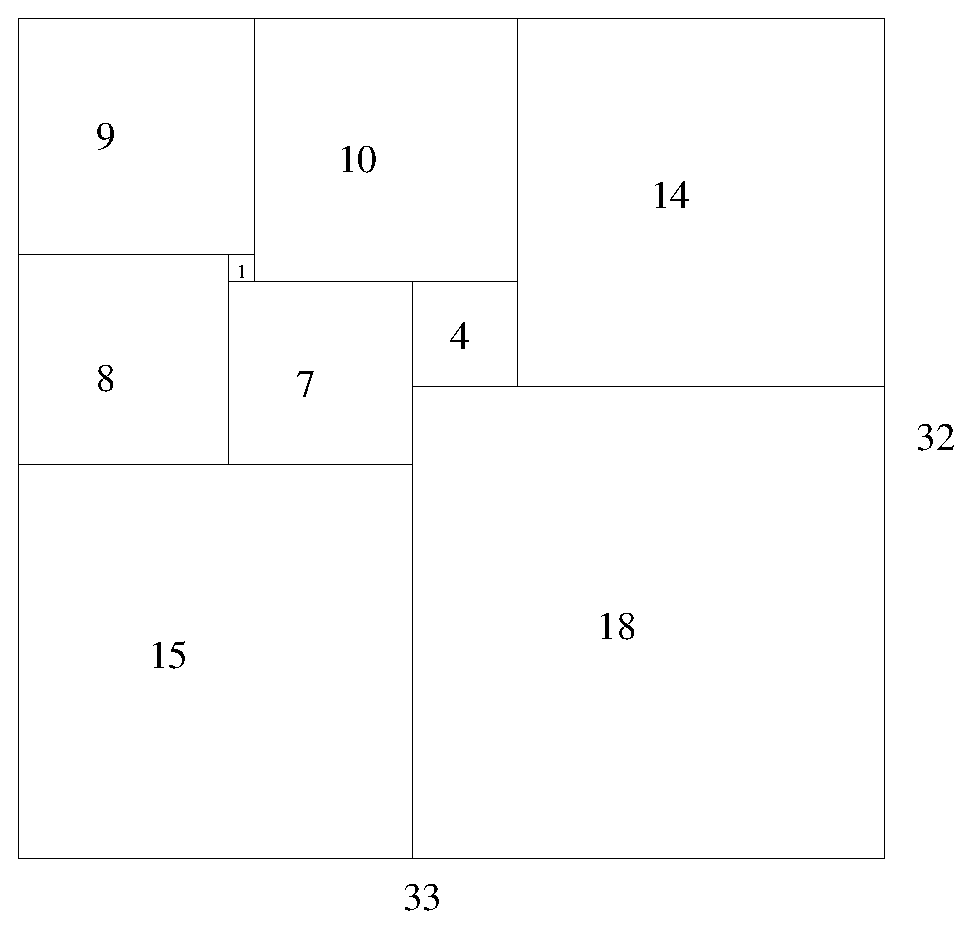
\epsfig{file=tokeletes.eps,width=0.4\textwidth}
\end{center}

A feladat megoldása során a négyzetet a ,,tetris-elv'' alapján, alulról
felfelé és balról jobbra fogjuk kitölteni, tehát a következő négyzetet
mindig igyekszünk a négyzetben lent és bal oldalt elhelyezni, ameddig
ez lehetséges. Mivel a fenti elv alapján töltjük ki a négyzetet, ezért a
ki nem töltött terület összefüggő, ezért jellemezhető a körvonalával, amit
Prologban egy listával fogunk lekódolni, amelyben a vonal függőleges és
vízszintes szakaszainak hosszát adjuk meg egy adott körüljárási sorrend
szerint. A függőleges és vízszintes szakaszok váltakozva fordulnak elő,
ezért a listánkban minden páratlanadik elem függőleges szakaszt, minden
párosadik elem vízszintes szakaszt fog kódolni. A körüljárást a négyzet
bal felső sarkából kezdjük az óramutató járásával ellenkező irányban, és
a lista utolsó elemét elhagyjuk, mivel a körvonal záródása miatt ez úgyis
redundáns. Ezek alapján például egy 33 $\times$ 32-es üres négyzet a
\cd{[-32,33,32]} listával kódolható. Ha tekintjük a fenti négyzetet abban
az állapotban, amikor csak a 15 oldalhosszúságú négyzetet helyeztük el,
akkor az üres területet a \cd{[-17,15,-15,18,32]} lista írja le.
\br
A keresési terünkben kétfajta választási pont fog előfordulni: vízszintes
és függőleges. Függőleges választási pontnál azt döntjük el, hogy amikor
egy négyzet mellé egy másik négyzetet lerakunk, akkor az új négyzet magassága
milyen relációban álljon a már lerakott négyzettel. Vízszintes választási
pontnál azt döntjük el, hogy a már kiválasztott oldalhosszúságú négyzet
mellett mekkora üres helyet hagyjunk még a kitöltésben. Ezt a két választási
pontot szemlélteti az alábbi ábra:

\begin{center}
\begin{tabular}{cc}
Vízszintes választási pont & Függőleges választási pont
\\
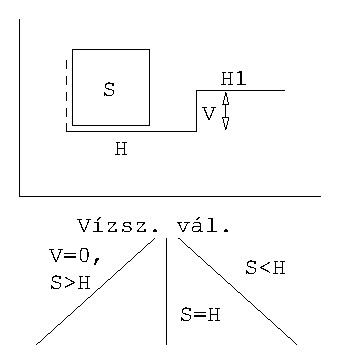
\epsfig{file=rect_choice_v.eps,width=0.4\textwidth}
&
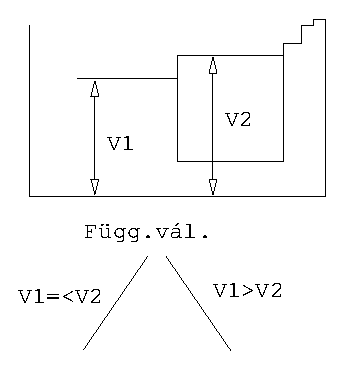
\epsfig{file=rect_choice_f.eps,width=0.4\textwidth}
\end{tabular}
\end{center}

A fentiekhez még annyi kiegészítés szükséges, hogy a programban a
négyzet függőleges oldalát mindig 1-nek választjuk, így csak a vízszintes
oldal méretével kell variálni. A megoldáshoz használt predikátumok:

\begin{verbatim}
% Colmerauer A.: An Introduction to Prolog III, 
% Communications of the ACM, 33(7), 69-90, 1990. 
\end{verbatim}
\begin{verbatim}
% Rectangle 1 x Width is covered by distinct 
% squares with sizes Ss.
filled_rectangle(Width, Ss) :-
       { Width >= 1 }, distinct_squares(Ss),
       filled_hole([-1,Width,1], _, Ss, []).
\end{verbatim}
\begin{verbatim}
% distinct_squares(Ss): All elements of Ss are distinct.
distinct_squares([]).
distinct_squares([S|Ss]) :-
       { S > 0 }, outof(Ss, S), distinct_squares(Ss).
\end{verbatim}
\begin{verbatim}
outof([],     _).
outof([S|Ss], S0) :- { S =\= S0 }, outof(Ss, S0).
\end{verbatim}
\begin{verbatim}
% filled_hole(L0, L, Ss0, Ss): Hole in line L0
% filled with squares Ss0-Ss (diff list) gives line L.
% Def: h(L): sum of lengths of vertical segments in L.
% Pre: All elements of L0 except the first >= 0.
% Post: All elems in L >=0, h(L0) = h(L).
filled_hole(L, L, Ss, Ss) :-
       L = [V|_], {V >= 0}.
filled_hole([V|HL], L, [S|Ss0], Ss) :-
       { V < 0 }, placed_square(S, HL, L1),
       filled_hole(L1, L2, Ss0, Ss1), { V1=V+S },
       filled_hole([V1,S|L2], L, Ss1, Ss).
\end{verbatim}
\begin{verbatim}
% placed_square(S, HL, L): placing a square size S on
% horizontal line HL gives (vertical) line L.
% Pre: all elems in HL >=0
% Post: all in L except first >=0, h(L) = h(HL)-S.
placed_square(S, [H,V,H1|L], L1) :- 
       { S > H, V=0, H2=H+H1 }, 
       placed_square(S, [H2|L], L1).
placed_square(S, [S,V|L], [X|L]) :- { X=V-S }.
placed_square(S, [H|L], [X,Y|L]) :- 
       { S < H, X= -S, Y=H-S }.
\end{verbatim}

A program belépési pontja a \cd{filled_rectangle/2} predikátum, amely
a \cd{Width} paraméterében fogja megadni a téglalap szélességét, \cd{Ss}-ben
pedig a kitöltéshez felhasznált négyzetek listáját. A \cd{distinct_squares/1}
korlát adja meg, hogy a négyzeteknek nem lehetnek azonos méretűek. Ez egy
egyszerű ,,darálás'' az \cd{Ss} listában előforduló összes négyzet-párra
az \cd{outof/2} segítségével. A négyzetek elhelyezését a \cd{filled_hole/4}
predikátum végzi. A predikátum harmadik és negyedik paramétere a kezdő-
és a végállapotban elhelyezett négyzetek listáját adja, az első és a második
paraméter pedig a harmadik és negyedik paraméterben leírt állapothoz tartozó
határoló vonalak leírása a fentebb leírt formában. A \cd{placed_square/3}
predikátum pedig a vízszintes választási pontok három fajtáját írja le,
mégpedig azt, hogy ilyen esetben a határoló vonal milyen szabályok szerint
változik.
\br
Lássunk egy példafuttatást:
\begin{verbatim}
% 600 MHz Pentium III
| ?-    length(Ss, N), N > 1, statistics(runtime, _),
        filled_rectangle(Width, Ss), 
        statistics(runtime, [_,MSec]).

N = 9, MSec = 8010, Width = 33/32,
Ss = [15/32,9/16,1/4,7/32,1/8,7/16,1/32,5/16,9/32] ? ;

N = 9, MSec = 1010, Width = 69/61,
Ss = [33/61,36/61,28/61,5/61,2/61,9/61,25/61,7/61,16/61] ? ;

N = 9, MSec = 10930, Width = 33/32,
Ss = [9/16,15/32,7/32,1/4,7/16,1/8,5/16,1/32,9/32] ? 
\end{verbatim}
Amint látható, 9-nél kevesebb négyzettel nem lehet lefedni a téglalapot,
9-re viszont máris három megoldást talált a program, ebből az első és
a harmadik csak a négyzetek elhelyezésében különbözik.
\br
A program működésének megértéséhez hagyjuk ki az \cd{outof/2} által
generált korlátokat, és nézzük meg, hogy kisebb méretű téglalapokra milyen
korlátokat generál a program! Kommentként közöljük az adott ágon generált
korlátokat és lefedést, a rendundáns korlátok elhagyásával. A
\cd{filled_rectangle/3} \cd{[eqsq]} paramétere jelzi, hogy most megengedünk
azonos méretű négyzeteket.
\begin{verbatim}
| ?- filled_rectangle(W, [S1,S2,S3], [eqsq]).

S1 = 1/2, S2 = 1, S3 = 1/2, W = 3/2 ? ;    % 3 3 2 2 2 2
                                           % 3 3 2 2 2 2
% {W=S1+S2}, {S2=<1}, {S1=S3},             % 1 1 2 2 2 2
% {S2>=S1+S3}, {S1+S3>=1}.                 % 1 1 2 2 2 2

S1 = 1, S2 = 1/2, S3 = 1/2, W = 3/2 ? ;    % 1 1 1 1 3 3
                                           % 1 1 1 1 3 3
% {W=S1+S2}, {S2=S3}, {S2+S3=<1},          % 1 1 1 1 2 2
% {S2+S3>=S1}, {S1>=1}.                    % 1 1 1 1 2 2

S1 = 1, S2 = 1, S3 = 1, W = 3 ? ; no

% {W=S1+S2+S3}, {S3=<1}, {S3>=S2},         % 1 1 2 2 3 3 
% {S2>=S1}, {S1>=1}.                       % 1 1 2 2 3 3 
\end{verbatim}

 % A SICStus clpq és clpr könyvtárai
\clearpage

\section{A SICStus \clpb könyvtára}

A következõ fejezetben a SICStus \clpb könyvtárával fogunk foglalkozni.
A \clpb könyvtárat az alábbi módon lehet használatba venni:
\begin{verbatim}
:- use_module(library(clpb)).
\end{verbatim}

\subsection{A \clpb könyvtár általános jellemzése}

A \clpb könyvtár a kétértékû Boole-logikán alapuló CLP rendszert valósít meg,
ennek megfelelõen a \clpb változók értékkészlete a ${0,1}$ halmaz.

\enumhead{Felhasználható függvények (egyben korlát-relációk)}
\btab{lp{30em}}
\cd{{\~{}} P}      &  \cd{P} hamis ({\it negáció}).\\
\cd{P * Q}     &  \cd{P} és \cd{Q} mindegyike igaz ({\it konjunkció}).\\
\cd{P + Q}     &  \cd{P} és \cd{Q} legalább egyike igaz ({\it
diszjunkció}).\\
\cd{P \# Q}    &  \cd{P} és \cd{Q} pontosan egyike igaz ({\it kizáró
vagy}).\\
\cd{X {\^{}} P}  &  Létezik olyan \cd{X}, hogy \cd{P} igaz (azaz \cd{P[X/0]+P[X/1]} igaz).\\
\verb'P =\= Q'  &  Ugyanaz, mint \verb'P # Q'.\\
\verb'P =:= Q'  &  Ugyanaz, mint \verb'~(P # Q)'.\\
\verb'P =< Q'   &  Ugyanaz, mint \verb'~P + Q'.\\
\verb'P >= Q'   &  Ugyanaz, mint \verb'P + ~Q'.\\
\verb'P < Q'    &  Ugyanaz, mint \verb'~P * Q'.\\
\verb'P > Q'    &  Ugyanaz, mint \verb'P * ~Q'.\\
\cd{card(Is, Es)} &  Az \cd{Es} listában szereplõ igaz értékû
kifejezések száma eleme az \cd{Is} által jelölt halmaznak (\cd{Is}
egészek és \cd{Tol-Ig} szakaszok listája).\\
\etab

A \Clpb -ben az összes korlát egyszerû korlát, nincsenek összetett korlátok.
Pont ez a tény az, ami a \Clpb -t nagy feladatok megoldására alkalmatlanná
teszi, hiszen minden korlát azonnal bekerül a korlát-tárba, és egy idõ után
a megoldó algoritmus (a Boole-egyesítés) mûködése a korlát-tár nagy mérete
miatt lelassul.

\enum{Alapvetõ könyvtári eljárások}{
\item \cd{sat(Kifejezés)} -- hozzáveszi \cd{Kifejezés}t a korlát-tárhoz.
\cd{Kifejezés} a \cd{0} és \cd{1} konstansokból, atomokból, valamint
változókból a fenti mûveletekkel felépített logikai kifejezés. A kifejezésben
elõforduló atomok a kifejezés legkülsõ szintjén univerzálisan kvantifikált
változókat jelentenek.

\item \cd{taut(Kifejezés,Érték)} -- megvizsgálja, hogy \cd{Kifejezés}
levezethetõ-e a korlát-tárból. Ha levezethetõ, akkor \cd{Érték}et \cd{1}-gyel
egyesíti. Ha \cd{Kifejezés} tagadása levezethetõ, akkor \cd{Érték}et \cd{0}-val
egyesíti. Minden más esetben meghiúsul.

\item \cd{labeling(Változók)} -- beállítja a \cd{Változók} lista összes
elemét 1-re vagy 0-ra úgy, hogy a korlát-tár teljesüljön. Visszalépésre az
összes lehetséges megoldást felsorolja.
}

\subsection{Példafutások a \clpb könyvtár segítségével}

\begin{verbatim}
| ?- sat(X + Y).
sat(X=\=_A*Y#Y) ? 

| ?- sat(x + Y).
sat(Y=\=_A*x#x) ? 

| ?- taut(_A ^ (X=\=_A*Y#Y) =:= X+Y, T).
T = 1 ? 

| ?- sat(A # B =:= 0).
B = A ? 

| ?- sat(A # B =:= C), A = B.
B = A, C = 0 ? 

| ?- taut(A =< C, T).
no

| ?- sat(A =< B), sat(B =< C), taut(A =< C, T).
T = 1, sat(A=:=_A*_B*C), sat(B=:=_B*C) ? 
\end{verbatim}

Látható, hogy a \clpb a korlát-tár tartalmát \cd{sat(Kifejezés)} alakú
struktúrák konjunkciójaként jeleníti meg, ahol \cd{Kifejezés} mindig egy
,,polinom'', azaz konjunkciók kizáró vagy (\cd{\#}) mûveletekkel képzett
sorozata. Az atomok a fent elmondottak szerint univerzálisan kvantifikált
változókat jelentenek. Az univerzális és az egzisztenciális kvantifikáció
különbségének kiemelésére nézzük meg az alábbi példákat is:

\begin{alltt}
| ?- sat(~x+ ~y=:= ~(x*y)).   % \(\forall\cd{xy}(\lnot\cd{x}\lor\lnot\cd{y}=\lnot(\cd{x}\land\cd{y}))\)
yes
| ?- sat(~X+ ~Y=:= ~(X*Y)).   % \(\exists?\cd{XY}(\lnot\cd{X}\lor\lnot\cd{Y}=\lnot(\cd{X}\land\cd{Y}))\)
true ? ; no
| ?- sat(x=<y).               % \(\forall\cd{xy}(\cd{x} \to \cd{y})\)
no
| ?- sat(X=<y).               % \(\forall\cd{y}\exists?\cd{X}(\cd{X} \to \cd{y})\) 
sat(X=:=_A*y) ? ; no
\end{alltt}

Nézzünk most egy picit komplikáltabb \clpb példát, amely egy egy bites
összeadó áramkör mûködését próbálja modellezni \clpb korlátok segítségével:

\begin{verbatim}
| ?- [user].
| adder(X, Y, Sum, Cin, Cout) :-
     sat(Sum =:= card([1,3],[X,Y,Cin])),
     sat(Cout =:= card([2-3],[X,Y,Cin])).
| {user consulted, 40 msec 576 bytes}
yes
\end{verbatim}

Az összeadó mûködése a \cd{card/2} segítségével nagyon egyszerûen leírható:
az összeg értéke akkor 1, ha az \cd{[X,Y,Cin]} listában (\cd{Cin} a carry in,
tehát a bemenõ átvitel rövidítése) 1 vagy 3 db egyes van, \cd{Cout}
(a kimenõ átvitel) értéke pedig akkor 1, ha az \cd{[X,Y,Cin]} listában legalább
két db egyes van. Nézzük meg, hogy ezeket a korlátokat milyen formában tárolja
a \clpb rendszer!

\begin{verbatim}
| ?- adder(x, y, Sum, cin, Cout).
sat(Sum=:=cin#x#y),
sat(Cout=:=x*cin#x*y#y*cin) ?
\end{verbatim}

Látható, hogy a \cd{card/2} itt is konjunkciók kizáró vagy kapcsolatára
vezetõdött vissza. Mivel csak a \cd{Sum} és \cd{Cout} változók viselkedésére
voltunk kíváncsiak, ezért a másik három változót egzisztenciálisan
kvantifikáltuk. Nézzük meg azt az egyszerûsített esetet is, amikor \cd{Cin}-t
0-ra kötjük, tehát nincs bemenõ átvitel:

\begin{verbatim}
| ?- adder(x, y, Sum, 0, Cout).
sat(Sum=:=x#y),
sat(Cout=:=x*y) ?
\end{verbatim}

Ha a megoldás nem egyértelmû, akkor a \cd{labeling} eljárással tudjuk
felsoroltatni az összes lehetséges megoldást:

\begin{verbatim}
| ?- adder(X, Y, 0, Cin, 1), labeling([X,Y,Cin]).
Cin = 0, X = 1, Y = 1 ? ; 
Cin = 1, X = 0, Y = 1 ? ;
Cin = 1, X = 1, Y = 0 ? ;
no
\end{verbatim}

\subsection{A Boole-egyesítés}

A \clpb könyvtár két Boole-kifejezés egyesítésére ,,meglepõ módon'' a
Boole-egyesítés nevû algoritmust használja. A feladat pontos megfogalmazása:
legyen adott a $g$ és $h$ Boole-kifejezés, és keressük a $g = h$
egyenletet megoldó legáltalánosabb egyesítõt (a továbbiakban ezt $mgu(g,h)$-val
jelöljük). Mivel a $g = h$ egyenlet helyettesíthetõ a $g \oplus h = 0$ egyenlettel
(ahol $\oplus$ a kizáró vagy mûveletet jelenti, amit \Clpb -ben a \cd{\#}
operátor jelöl), ezért a továbbiakban a Boole-egyesítés vizsgálatához
elegendõ az $f=0$ alakú egyenletek megoldását vizsgálnunk. Az egyesítés
minden lépése során egy $f=0$-beli $x$ formulaváltozót szeretnénk kifejezni a
többi segítségével.
\br
Legyen $f_x(1)$ az $f$-bõl az $x=1$ helyettesítéssel, az $f_x(0)$ pedig az
$f$-bõl az $x=0$ helyettesítéssel kapott formula. $f=0$ kielégíthetõségének
szükséges feltétele $f_x(1) \land f_x(0) = 0$ kielégíthetõsége. Fejezzük ki
$x$-et $f_x(1)$ és $f_x(0)$ segítségével úgy, hogy $f=0$ legyen!

\btab{|l|l|l|}
\hline $f_x(0)$ & $f_x(1)$ & $x$ \\
\hline 0        & 0        & bármi ($w$)\\
\hline 0        & 1        & 0\\
\hline 1        & 0        & 1\\
\hline 1        & 1        & érdektelen\\
\hline
\etab

Ha $x$-et $x=(a \land \overline{w}) \oplus (b \land w)$ (Prolog: \cd{X=A*{\~{}}W \# B*W})
alakban keressük, akkor a fentiek szerint $a$ és $b$ értéke az alábbiak
szerint adódik:

\begin{center}
\begin{tabular}{|l|l|l||l|l|}
\hline $f_x(0)$ & $f_x(1)$ & $x$ & $a$ & $b$ \\
\hline 0        & 0        & $w$ & 0   & 1   \\
\hline 0        & 1        & 0   & 0   & 0   \\
\hline 1        & 0        & 1   & 1   & 1   \\
\hline
\end{tabular}
\end{center}

A táblázat alapján az $a=f_x(0)$ és $b=\overline{f_x(1)}$ megfeleltetés tûnik
a legegyszerûbbnek. Így alapján az egyesítési algoritmus mûködése az $f=0$
alakú egyenlõségekre:

\begin{enumerate}
\item Ha $f$-ben nincs változó, akkor $f$-nek azonosan 0-nak kell lennie,
      egyébként ugrás a következõ pontra.
\item Helyettesítsünk $f$-ben egy tetszõleges $x$ változót az
      $x=(f_x(0) \land \overline{w}) \oplus (\overline{f_x(1)} \land w)$ kifejezéssel
      (Prolog: \cd{X=}$f_x(0)$\cd{*{\~{}}W \# {\~{}}}$f_x(1)$\cd{*W}).
\item Folytassuk az egyesítést az $f_x(1) \land f_x(0) = 0$ egyenlõségre
\end{enumerate}

Példák a Boole-egyesítésre:

\begin{itemize}
\item $mgu$(\cd{X+Y}, \cd{0}) $\longrightarrow$ \cd{X = 0, Y = 0};
\item $mgu$(\cd{X+Y}, \cd{1}) = $mgu$(\verb'~(X+Y)', \cd{0})
$\longrightarrow$ \cd{X = W * Y \# Y \# 1};
\item $mgu$(\cd{X*Y}, \verb'~(X*Z)') = $mgu$(\cd{(X*Y)\#(X*Z)\#1}, \cd{0})
$\longrightarrow$ \cd{X = 1}, \cd{Y = {\~{}}Z}.
\end{itemize}

\subsection{A \clpb belsõ ábrázolási formája}

A \clpb könyvtár a Boole-kifejezéseket az úgynevezett \emph{Boole/bináris
döntési diagram}ok (\emph{Boole/Binary Decision Diagram}s, \emph{BDD})
segítségével ábrázolja. Ezek irányított körmentes gráfok (\emph{directed
acyclic graph}, \emph{DAG}), amelyekben kétféle csomópont és kétféle él
szerepel. A csomópontok tartozhatnak változóhoz vagy a 0 és 1 konstansokhoz.
Csak a változókat tartalmazó csomópontokból indulhat ki él, mégpedig
mindkettõbõl kétfajta, az egyik a hamis értéknek (az ábrákon szaggatott vonal),
a másik az igaz értéknek (az ábrákon folytonos vonal) felel meg. Az egyik
csomópont kitüntetett abból a szempontból, hogy ebbe a csomópontba egy
végpont nélküli él is befut (ezt a csomópontot hívjuk \emph{kezdõ csomópont}nak).
A BDD-k segítségével meghatározható az általuk reprezentált Boole-kifejezés
értéke. Ehhez a gráfot a kezdõ csomópontból kezdve kell bejárni a
következõ szabályok szerint:

\begin{enumerate}
\item Ha az aktuális csomópont a 0 vagy az 1 konstansot tartalmazza, akkor
megállhatunk a bejárással, és a kifejezés értéke 0 vagy 1, a csomópont
tartalmától függõen.
\item Ha az aktuális csomópont változót tartalmaz, akkor a változó aktuális
értékétõl függõen vagy a szaggatott (0-nak megfelelõ), vagy a folytonos
(1-nek megfelelõ) él mentén kell folytatni a bejárást.
\end{enumerate}

Mivel a gráf irányított, körmentes, és csak a 0-t vagy 1-et tartalmazó
csomópontok nyelõk, ezért az algoritmus véges idõn belül le fog futni.
A könnyebb érthetõség kedvéért álljon itt két Boole-kifejezés bináris döntési
diagramja:

\btab{cp{1.5cm}c}
\verb'(X+Y) # 1' & & \verb'X*Y # X*Z # 1'  \\
\hspace*{1cm}\raisebox{2cm}{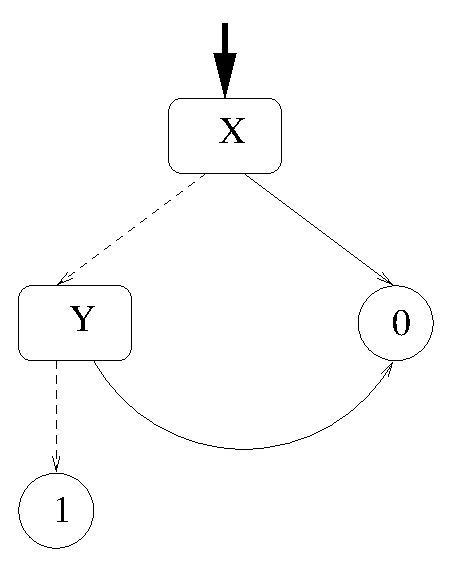
\epsfig{file=bdd2.eps, width=0.23\linewidth}} & & 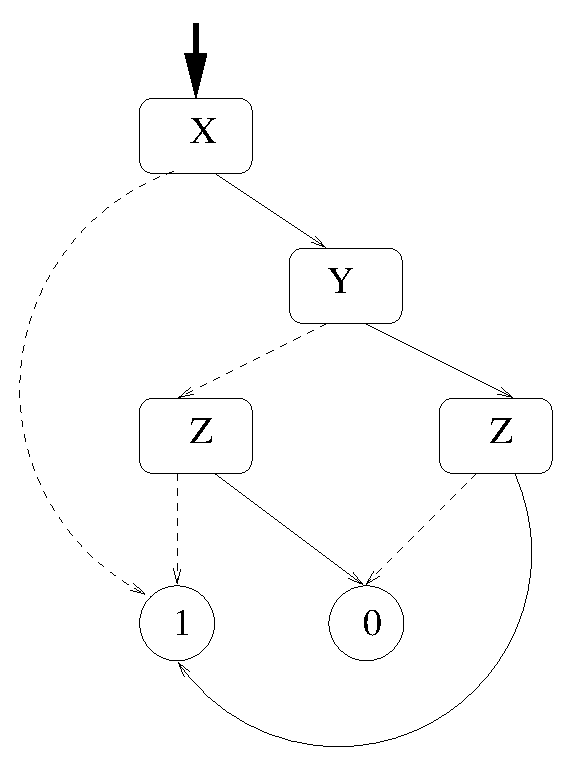
\epsfig{file=bdd1.eps, width=0.3\linewidth}  \\
\etab

\subsection{Összetett \clpb példa: hibakeresés áramkörben}

Legyen adott egy egybites összeadó áramköri modellje (funkcionális elemekkel
és összeköttetésekkel). Írjunk egy olyan \clpb programot, amely adott
bemenet-kimenet párra megmondja, hogy melyik funkcionális elem mûködik
hibásan, ha feltételezzük, hogy egyszerre csak egy hibásodik meg!

\begin{center}\insertfig{adder1}{10cm}\end{center}

\begin{verbatim}
fault([F1,F2,F3,F4,F5], [X,Y,Cin], [Sum,Cout]) :-
        sat(
                    card([0-1],[F1,F2,F3,F4,F5]) *
                    (F1 + (U1 =:= X * Cin)) *
                    (F2 + (U2 =:= Y * U3)) *
                    (F3 + (Cout =:= U1 + U2)) *
                    (F4 + (U3 =:= X # Cin)) *
                    (F5 + (Sum =:= Y # U3))
                ).
\end{verbatim}

Amint látható, a \cd{fault/3} predikátumban semmi mást nem tettünk, mint
specifikáltuk az egyes áramköri elemek mûködését, valamint a \cd{card}
segítségével megadtuk azt a tényt is, hogy egyszerre legfeljebb egy
áramköri elem hibás. Lássunk néhány példát a \cd{fault} mûködésére!

\begin{verbatim}
| ?- fault(L, [1,1,0], [1,0]).
                            L = [0,0,0,1,0] ? ;  no
\end{verbatim}

Itt a \cd{fault} helyesen kikövetkeztette, hogy ilyen bemenet-kimenet
pár esetén csak a 4. funkcionális elem, azaz a programkód alapján
az \cd{X}-re és \cd{Cin}-re kapcsolódó XOR kapu lehet hibás.

\begin{verbatim}
| ?- fault(L, [1,0,1], [0,0]).
                            L = [_A,0,_B,0,0],
                            sat(_A=\=_B) ? ; no
\end{verbatim}

Itt a \cd{fault} úgy gondolja, hogy vagy az elsõ, vagy a harmadik funkcionális
elem a hibás, ezt a korlát-tárban lévõ \cd{sat(_A=\bs=_B)} fejezi ki. Ha
ehelyett látni szeretnénk a két lehetõséget teljesen behelyettesített
változókkal, akkor szükséges a \cd{labeling} használata is:

\begin{verbatim}
| ?- fault(L, [1,0,1], [0,0]), labeling(L).
                            L = [1,0,0,0,0] ? ;
                            L = [0,0,1,0,0] ? ; no
\end{verbatim}

Végül megkérdezhetjük a \cd{fault}-tól, hogy helyes áramköri mûködést
feltételezve mik az egyes kimenetekhez rendelhetõ logikai egyenletek:

\begin{verbatim}
| ?- fault([0,0,0,0,0], [x,y,cin], [Sum,Cout]).
                            sat(Cout=:=x*cin#x*y#y*cin),
                            sat(Sum=:=cin#x#y) ? ; no
\end{verbatim}

Tekintsünk most egy XOR kaput megvalósító tranzisztoros áramkört, és
valósítsuk meg ennek a verifikációját \clpb programmal!

\begin{center}\insertfig{xor}{8cm}\end{center}

Elõször leírjuk az npn és pnp tranzisztorok mûködését \clpb kifejezésekkel:
\begin{verbatim}
n(D, G, S) :-    % Gate => Drain = Source
        sat( G*D =:= G*S).

p(D, G, S) :-    % ~ Gate => Drain = Source
        sat( ~G*D =:= ~G*S).
\end{verbatim}

Ezek segítségével megfogalmazhatjuk az XOR kapu mûködését, ha a földelést
0-val, a tápfeszültséget 1-gyel jelöljük:

\begin{verbatim}
xor(A, B, Out) :-
        p(1, A, X),
        n(0, A, X),
        p(B, A, Out),
        n(B, X, Out),
        p(A, B, Out),
        n(X, B, Out).
\end{verbatim}

Ellenõrizzük, hogy az npn és pnp tranzisztorokra felírt egyenleteink
helyesen mûködnek-e a gate feszültség ki- és bekapcsolására:

\begin{verbatim}
| ?- n(D, 1, S).                 S = D ?
| ?- n(D, 0, S).                 true ?
| ?- p(D, 0, S).                 S = D ?
| ?- p(D, 1, S).                 true ?
\end{verbatim}

A fentiek szerint a tranzisztorok logikai felírása helyes, így nem
maradt más hátra, mint hogy ellenõrizzük, hogy az XOR kapu ténylegesen
az XOR függvényt valósítja-e meg:

\begin{verbatim}
| ?- xor(a, b, X).               sat(X=:=a#b) ?
\end{verbatim}

\subsection{Aknakeresõ játék \Clpb -ben}

Az alábbi programkód egy aknakeresõ játékot valósít meg \clpb programkód
formájában.

\begin{verbatim}
:- use_module([library(clpb),library(lists)]).
\end{verbatim}
\begin{verbatim}
mine(Rows, Cols, Mines, Bd) :-
        length(Bd, Rows), all_length(Bd, Cols), 
        append_lists(Bd, All),
        sat(card([Mines], All)), play_mine(Bd, []).
\end{verbatim}
\begin{verbatim}
all_length([], _).
all_length([L|Ls], Len) :- 
        length(L, Len), all_length(Ls, Len).
\end{verbatim}
\begin{verbatim}
append_lists([], []).
append_lists([L|Ls], Es) :-
        append_lists(Ls, Es0), append(L, Es0, Es).
\end{verbatim}
\begin{verbatim}
play_mine(Bd, Asked) :- 
        select_field(Bd, Asked, R, C, E), !,
        format('Row ~w, col ~w (m for mine)? ', [R,C]), 
        read(Ans), process_ans(Ans, E, R, C, Bd), 
        play_mine(Bd, [R-C|Asked]).
play_mine(_Bd, _Asked).
\end{verbatim}
\begin{verbatim}
select_field(Bd, Asked, R, C, E) :-
        nth(R, Bd, L), nth(C, L, E), 
        non_member(R-C, Asked), taut(E, 0), !.
select_field(Bd, Asked, R, C, E) :-
        nth(R, Bd, L), nth(C, L, E), 
        non_member(R-C, Asked), \+ taut(E,1), !.
\end{verbatim}
\begin{verbatim}
process_ans(m, 1, _, _, _) :- 
        format('Mine!~n', []), !, fail.
process_ans(Ans, 0, R, C, Bd) :-
        integer(Ans), neighbs(n(R, C, Bd), Ns), 
        sat(card([Ans], Ns)).
\end{verbatim}
\begin{verbatim}
neighbs(RCB, N7) :-
        neighbour(-1,-1, RCB, [], N0), 
        neighbour(-1, 0, RCB, N0, N1),
        neighbour(-1, 1, RCB, N1, N2), 
        neighbour( 0,-1, RCB, N2, N3),
        neighbour( 0, 1, RCB, N3, N4), 
        neighbour( 1,-1, RCB, N4, N5),
        neighbour( 1, 0, RCB, N5, N6), 
        neighbour( 1, 1, RCB, N6, N7).
\end{verbatim}
\begin{verbatim}
neighbour(ROf, COf, n(R0, C0, Bd), Nbs, [E|Nbs]) :-
        R is R0+ROf, C is C0+COf, 
        nth(R, Bd, Row), nth(C, Row, E), !.
neighbour(_, _, _, Nbs, Nbs).
\end{verbatim}

A játék belépési pontja a \cd{mine(Rows,Cols,Mines,Bd)} eljárás, amely
egy \cd{Rows} $\times$ \cd{Cols} méretû táblát készít el a \cd{Bd}
listában, és felteszi róla, hogy \cd{Mines} db 1-es van benne.
Ezek után a \cd{play_mine/2} eljáráson keresztül kijelzi, hogy melyik
mezõ tartalmára kíváncsi, erre a felhasználónak az \cd{m.} karaktersorozattal
kell válaszolnia, ha akna van ott, üres mezõ esetén pedig meg kell adni, hogy
hány akna található a mezõ körül. Ha a felhasználó válasza \cd{m.}, akkor a
program szomorúan konstatálja, hogy veszített (\cd{Mine!}), ha viszont egy
szám, akkor a tippelt mezõ körül lévõ mezõkre a \cd{process_ans/5} eljárás
második klózával felveszi a megfelelõ számossági korlátot. A következõ tipp
kiválasztását a \cd{select_field/5} eljárás végzi, ez mindig egy olyan mezõt
választ ki, amelyrõl a program egyértelmûen tudja, hogy üres (1. klóz), ha ilyet
nem talál, akkor pedig egy olyat, amelyrõl nem tudja biztosan, hogy aknát tartalmaz
(2. klóz). Egy egyszerû példajáték ($3 \times 3$-as tábla, akna a 2. sor 1. mezõjén
és a 3. sor 3. mezõjén van):

\begin{verbatim}
| ?- mine(3,3,2,Bd).
% az elsõ két lépésben a program csak reménykedik abban, hogy
% nem lép aknára
Row 1, col 1 (m for mine)? 1.
Row 1, col 2 (m for mine)? 1.
% itt a program már rájön, hogy az (1,3) és a (2,3) mezõ üres
Row 1, col 3 (m for mine)? 0.
% ebbõl már azt is tudja, hogy a (2,2) mezõ üres, így viszont
% a (2,1) mezõn akna van
Row 2, col 2 (m for mine)? 2.
% mivel a (2,3) mezõrõl már elõzõleg kikövetkeztette, hogy üres,
% ezért azt is meg meri kérdezni
Row 2, col 3 (m for mine)? 1.
% mivel a (2,2) mezõ körül már csak 1 akna helyét nem tudjuk,
% de azt is tudjuk, hogy a (2,3) mezõ körül is 1 akna van, ezért
% a (3,1) mezõn nem lehet akna
Row 3, col 1 (m for mine)? 1.
% így viszont a (3,2) mezõ is üres
Row 3, col 2 (m for mine)? 2.
Bd = [[0,0,0],[1,0,0],[0,0,1]] ? ;
no
\end{verbatim}

Vegyük észre, hogy a program inkonzisztens adatok esetén meghiúsulást produkál:

\begin{verbatim}
| ?- mine(3,3,2,Bd).
Row 1, col 1 (m for mine)? 1.
Row 1, col 2 (m for mine)? 1.
Row 1, col 3 (m for mine)? 0.
Row 2, col 2 (m for mine)? 1.
no
\end{verbatim}

A \clpb mohósága miatt azonban a program egy $20 \times 20$-as aknamezõre már
nagyon hosszú ideig veszi fel a \cd{mine/4}-ben szereplõ \cd{sat(card...)}
korlátot (mivel a \cd{card}-ot is ,,polinom'' formára vezeti vissza a listában
szereplõ összes változó esetén), ilyenkor a program szinte játszhatatlanul lassú lesz. % A SICStus clpb könyvtára
\clearpage

\section{A SICStus \clpfd könyvtára}

A következõ fejezetben a SICStus \clpfd könyvtárával fogunk foglalkozni.
A \clpfd könyvtárat az alábbi módon lehet használatba venni:
\begin{verbatim}
:- use_module(library(clpfd)).
\end{verbatim}

\subsection{A \clpfd könyvtár általános jellemzése}

A \clpfd könyvtár az egész számok véges tartományain (\emph{finite domain, FD})
alapuló CLP rendszert valósít meg. A könyvtár általános alapelve, hogy a
CLP relációkat a \cd{\#} jellel kell kezdeni, ezzel különböztetve meg õket
a hagyományos Prolog jelektõl.

\enum{Felhasználható függvények}{
\item kétargumentumúak: {\tt +, -, *, /, mod, min, max}
\item egyargumentumú: {\tt abs} \\
Ezek a hagyományos matematikai mûveletekkel megegyezõ funkcióval rendelkeznek.
}
\enum{Felhasználható relációk}{
\item aritmetikaiak: \cd{\#<, \#>, \#=<, \#>=, \#= \#\bs=}\\
Ezek a jól ismert Prolog relációjelek megfelelõi, mindegyik \cd{xfx 700}
típusú operátor.
\item halmazmûveletek:
\begin{itemize}
  \item \cd{\var{X} in \var{Halmaz}} ---
     \cd{\var{X}} értékét \cd{\var{Halmaz}}-ból veszi
  \item \cd{domain([\var{Változók},\ldots], \var{Min}, \var{Max})} ---
     \cd{\var{Változók}} minden változója értékét a
     \cd{\var{Min}}..\cd{\var{Max}} intervallumból veszi
\end{itemize}
ahol \cd{\var{Halmaz}} lehet:
\begin{itemize}
\item felsorolás: \cd{\{\var{Szám},\ldots\}}
\item intervallum: \cd{\var{Min}..\var{Max}} (\cd{xfx 550} operátor)
\item két halmaz metszete: \cd{\var{Halmaz} \cd{/\bs} \var{Halmaz}}
    (\cd{yfx 500} beépített operátor)
\item két halmaz uniója: \cd{\var{Halmaz} \cd{\bs/} \var{Halmaz}}
    (\cd{yfx 500} beépített operátor)
\item egy másik halmaz komplemense: \cd{\bs\var{Halmaz}}
    (\cd{fy 500} operátor)
\end{itemize}
}

\cd{\var{Min}}-re megengedett az \cd{inf} névkonstans, ami az alsó korlát
hiányát jelenti ($-\infty$), hasonlóan \cd{\var{Max}}-ra megengedett a \cd{sup}
névkonstans, ami pedig a felsõ korlát hiányát jelenti ($+\infty$). A végtelen
korlátok általában csak kényelmi célokat használnak abban az esetben, ha
a tényleges korlátok kikövetkeztethetõek. Effektíven végtelen korlátokkal
rendelkezõ változóknak nem sok értelmük van, mert azok a címkézés (ld. késõbb)
során végtelen választási pontot hoznának létre (éppen ezért nem lehet olyan
változókat címkézni, amelyek végtelen tartománnyal rendelkeznek).
\br
A \clpfd világban egyszerû korlátoknak csak az \cd{\var{X} $\in$ \var{Halmaz}}
jellegû korlátokat tekintjük, minden más összetett korlátnak számít, éppen
ezért nagyon nagy hangsúly van az összetett korlátok erõsítõ tevékenységén
(ellentétben a \Clpb -vel, ahol nem is voltak összetett korlátok). Ez a tény
(illetve a \clpfd ,,lustasága'') teszi lehetõvé azt, hogy nagyobb problémákat
is megoldjunk vele. Az összetett korlátok erõsítõ tevékenysége a mesterséges
intelligencia-kutatások CSP (Constraint Satisfactory Problems) ágának
módszerein alapul.

Egy egyszerû \clpfd példa:

\begin{verbatim}
| ?- X in (10..20)/\ (\{15}), Y in 6..sup, Z #= X+Y.
X in(10..14)\/(16..20), Y in 6..sup, Z in 16..sup ? 
\end{verbatim}
\begin{verbatim}
| ?- X in 10..20, X #\= 15, Y in {2}, Z #= X*Y.
   Y = 2, X in(10..14)\/(16..20), Z in 20..40 ? 
\end{verbatim}

A második példán lustaságon kaphatjuk rajta a \clpfd következtetõ mechanizmust:
ugyan kikövetkeztethetõ lenne, hogy \cd{Z} csak 20 és 40 közötti \emph{páros}
szám lehet (mivel \cd{Y} páros, és \cd{X} 10 és 20 között van), sõt még
az is, hogy \cd{Z} semmiképp nem lehet 30 (mert \cd{X} sem lehet 15),
de ezt a \clpfd nem teszi meg, helyette egyszerûen megnézi \cd{X} alsó és
felsõ határát (10 és 20), ezeket beszorozza \cd{Y} alsó és felsõ határával
(ez jelen esetben azonos: 2 és 2), majd az így kapott négy szám minimuma és
maximuma által megadott intervallumra szûkíti \cd{Z}-t. Ezt a mechanizmust
\emph{intervallum-szûkítés}nek nevezzük, és az \ref{szukites} fejezetben
részletesen foglalkozunk majd vele.

\subsection{A \clpfd feladatok megoldási struktúrája}

Minden \clpfd feladat megoldása hasonló struktúrájú programot eredményez,
ezért érdemes megkülönböztetnünk a megoldási folyamat fõ lépéseit:

\begin{enumerate}
\item {\bf A probléma leképezése a \clpfd világra} \\
    Ebben a lépésben a problémának egy olyan modelljét kell megalkotnunk,
    amelyben a probléma egyes elemeit \clpfd fogalmakra (változókra,
    értéktartományokra) képezzük le.

\item {\bf Változók és korlátok felvétele} \\
    Ebben a lépésben be kell vezetnünk a feladatban szereplõ változókat,
    és fel kell vennünk a változók között fennálló korlát-relációkat.

\item {\bf Címkézés} \\
    Ha a problémának a korlátok alapján nincs egyértelmû megoldása, vagy
    ezt a rendszer nem tudta kikövetkeztetni, akkor a változókat el kell
    kezdenünk szisztematikusan az értéktartományaik egy-egy lehetséges
    értékéhez kötni, így meg fogjuk kapni a probléma összes megoldását.
    A címkézési folyamat a \clpb könyvtárnál látotthoz hasonló módon
    mûködik, de itt egy változó nem csak kétfajta értéket vehet fel.
    Ha a problémának a korlátok felvétele után már egyértelmû a megoldása,
    akkor a címkézési fázis elmarad.
\end{enumerate}

Lássuk a fent elmondottakat egy konkrét példán! A feladat az alábbi térkép
kiszínezése kék, piros és sárga színekkel úgy, hogy a szomszédos országok
különbözõ színûek legyenek, és ha két ország határán a \cd{<} jel van, akkor
a két szín ábécé-rendben a megadott módon kövesse egymást.

\begin{center}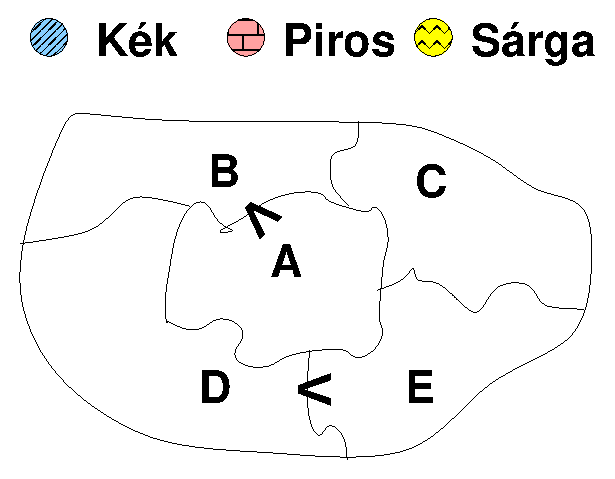
\epsfig{file=terkep.eps,width=0.2\textwidth}\end{center}

Egy lehetséges megoldási folyamat (\emph{zárójelben a CSP elnevezések}):

\begin{enumerate}
\item Minden mezõben elhelyezzük a három lehetséges színt ({\em változók és
tartományaik felvétele}).
\item Az ,,A'' mezõ nem lehet kék, mert annál ,,B'' nem lehetne kisebb.
A ,,B'' nem lehet sárga, mert annál ,,A'' nem lehetne nagyobb. Az ,,E'' és
,,D'' mezõk hasonlóan szûkíthetõk ({\em szûkítés, él-konzisztencia biztosítása}).
\item Ha az ,,A'' mezõ piros lenne, akkor mind ,,B'', mind ,,D'' kék lenne,
ami ellentmondás ({\em globális korlát, ill.\ borotválási technika}).
Tehát ,,A'' sárga. Emiatt a vele szomszédos ,,C'' és ,,E'' nem lehet sárga
({\em él-konszitens szûkítés}).
\item ,,C'' és ,,D'' nem lehet piros, tehát kék, így ,,B'' csak piros
lehet ({\em él-konszitens szûkítés}). Tehát az egyetlen megoldás:\\
A~=~sárga, B~=~piros, C~=~kék, D~=~kék, E~=~piros.
\end{enumerate}

Az alábbi ábrasorozaton láthatóak az egyes lépésekhez tartozó állapotok:

\btab{cccc}
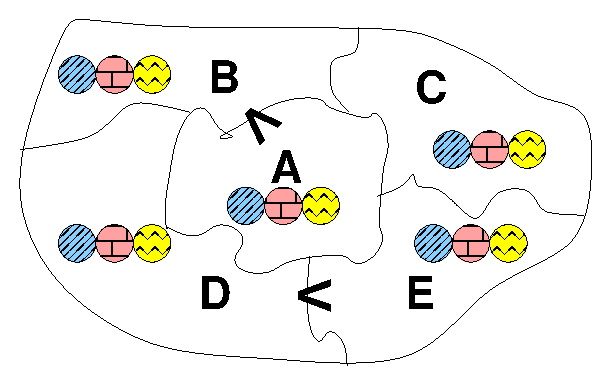
\epsfig{file=terkep2.eps,width=0.18\textwidth} &
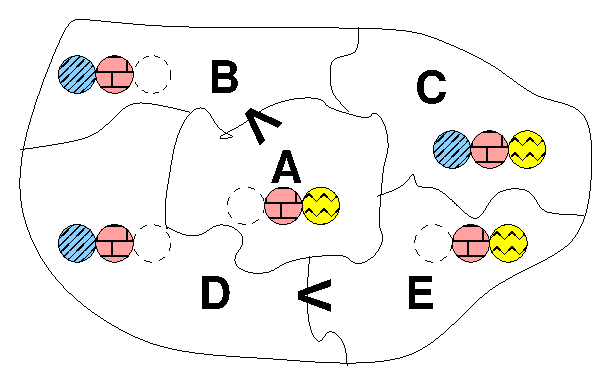
\epsfig{file=terkep3.eps,width=0.18\textwidth} &
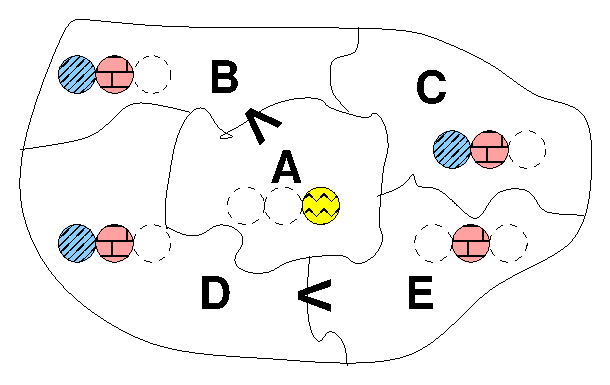
\epsfig{file=terkep4.eps,width=0.18\textwidth} &
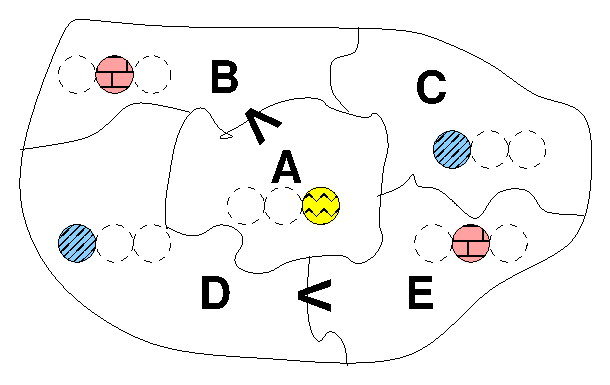
\epsfig{file=terkep5.eps,width=0.18\textwidth} \\
1. lépés & 2. lépés & 3. lépés & 4. lépés
\etab

\subsection{A CSP problémakör áttekintése}
\label{cspfogalmak}

Mint említettük, a \clpfd könyvtár a mesterséges intelligencia CSP megoldási
módszerein alapul, ezért mielõtt továbbmennénk, érdemes áttekinteni a CSP
problémakör fogalmait és eredményeit.

\enum{A CSP fogalma}{
\item Egy CSP-t egy $(X,D,C)$ hármassal jellemezhetünk, ahol
  \begin{itemize}
  \item $X = \tuple{x_1,\dots,x_n}$~--- változók
  \item $D = \tuple{D_1,\dots,D_n}$~--- tartományok, azaz nem üres halmazok
  \item $x_i$ változó a $D_i$ véges halmazból ($x_i$ tartománya) vehet fel
  értéket ($\forall i$-re $x_i \in D_i$)
  \item $C$ a problémában szereplõ korlátok (atomi relációk) halmaza,
  argumentumaik $X$ változói (például $C \ni c = r(x_1,x_3)$, $r \subseteq D_1 \times
  D_3$)
  \end{itemize}
\item A CSP feladat megoldása: minden $x_i$ változóhoz egy  $v_i\in D_i$
  értéket kell rendelni úgy, hogy minden $c\in C$ korlátot egyidejûleg
  kielégítsünk.
}

\definicio egy $c$ korlát egy $x_i$ változójának $d_i$ értéke
  \emph{felesleges}, ha nincs a $c$ többi változójának olyan értékrendszere,
  amely $x_i=d_i$-vel együtt kielégíti $c$-t.
\br
\tetel felesleges érték elhagyásával (szûkítés) ekvivalens CSP-t kapunk.
\br
\definicio egy korlát \emph{élkonzisztens} (\emph{arc consistent}),
  ha egyik változójának tartományában sincs felesleges érték. A CSP
  \emph{élkonzisztens}, ha minden korlátja élkonzisztens. Az élkonzisztencia 
  szûkítéssel biztosítható.
\br
Az \emph{élkonzisztencia} elnevezés onnan ered, hogy ha minden reláció
bináris, akkor a CSP probléma egy gráffal ábrázolható, ahol minden változónak
egy csomópont, minden relációnak egy él felel meg.

\enum{A CSP megoldás folyamata}{
\item felvesszük a változók tartományait;
\item felvesszük a korlátokat mint démonokat, amelyek szûkítéssel
él-konzisztenciát biztosítanak;
\item többértelmûség esetén címkézést (labeling) végzünk:
\begin{itemize}
\item kiválasztunk egy változót (pl.a legkisebb tartományút),
\item a tartományt két vagy több részre osztjuk (választási pont),
\item az egyes választásokat visszalépéses kereséssel bejárjuk
(egy tartomány üresre szûkülése váltja ki a visszalépést).
\end{itemize}
}

A térképszínezés, mint CSP feladat esetén minden országhoz egy változót
rendeltünk hozzá, ennek a változónak az értéke fogja az ország színét
kódolni. A színekhez ábécésorrend szerint az 1, 2, 3 értékek valamelyikét
rendeltük hozzá (kék $\to$ 1, piros $\to$ 2, sárga $\to$ 3), majd felvettük a
korlátokat egyrészt arra, hogy a szomszédos országok színei különböznek (ez a
változóértékek világában egy $\neq$ típusú relációt jelent), másrészt arra, hogy
az országok színei között megadott < relációk is teljesüljenek. Ezzel
kaptunk egy kiinduló korlát-gráfot, amit a felesleges élek elhagyásával
szûkítettünk. Az alábbi ábrán látható a kiinduló korlát-gráf és annak
élkonzisztens szûkített változata:

\btab{cp{5em}c}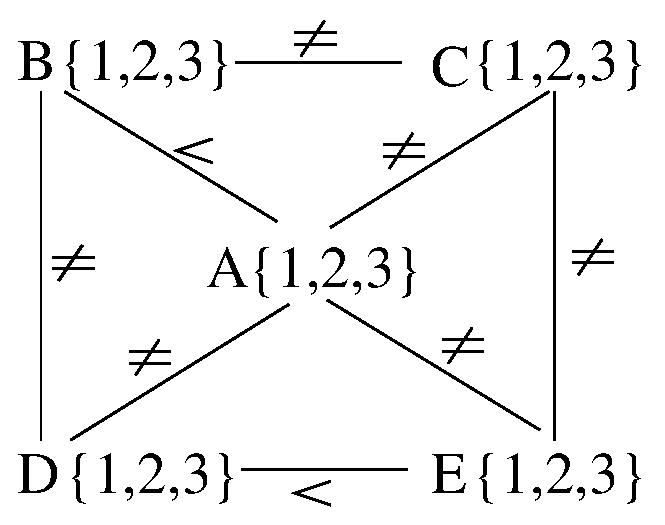
\epsfig{file=korlatok.eps,width=0.25\textwidth} & &
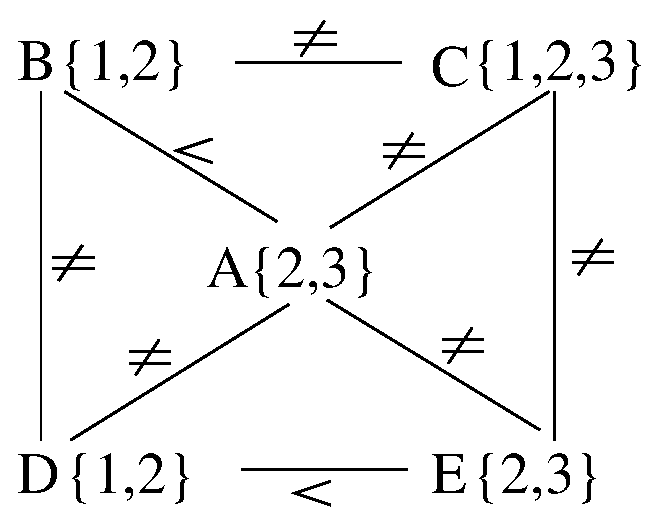
\epsfig{file=korlatok_elk.eps,width=0.25\textwidth}\etab

A CSP sémának a CLP világba történõ beágyazásával kapjuk a SICStusban lévõ
\clpfd könyvtárat. Minden CSP változónak egy \clpfd változó feleltethetõ meg,
a CSP változók értéktartományainak pedig egy-egy \clpfd egyszerû korlát.
A többi CSP korlát összetett \clpfd korlátként jelenik meg. A \clpfd korlát-tár
új változótartomány felvételén vagy egy meglévõ változó tartományának
szûkítésén módosulhat. Az összetett korlátok \emph{démon}ok lesznek, amelyek
hatásukat az \emph{erõsítés}en keresztül fejtik ki (ld. \ref{erosit} fejezet).
Az erõsítés mindig egyszerû korlátokat ad a korlát-tárhoz. A démonok ciklikusan
mûködnek: megszületnek, szûkítenek, elalszanak, aktiválódnak, szûkítenek,
elalszanak, \ldots aktiválódnak, szûkítenek, és amikor már levezethetõek a
korlát-tár tartalmából, akkor megszûnnek létezni. A démonokat mindig az
érintett korlátbeli változók tartományának módosulása aktiválja. A szûkítés
mértéke a démontól függ, néha nem elõnyös az összes lehetséges szûkítést
elvégezni, mert túlságosan költséges lenne.

\subsection{A \clpfd könyvtár jellegzetességei}

Ebben az alfejezetben a \clpfd könyvtár néhány jellegzetességét mutatjuk be
példákon keresztül. A példák megértéséhez egyetlen, nagyon fontos állítást
kell szem elõtt tartanunk: {\bf a \clpfd démonok csak a korlát-táron keresztül
hatnak egymásra!}
\br
A fenti mondat azt takarja, hogy a démonok nem ,,látják'' egymást, az
egymással való interakciójukat kizárólag a korlát-táron keresztül
végzik: az egyik démon szûkíti a korlát-tárat, ennek hatására egy
másik démon felébred, szûkít, erre egy harmadik démon ébred fel
és így tovább... Elõfordulhatnak azonban olyan esetek, amikor egyik
démon sem tud felébredni, és így esetleg egy nyilvánvaló ellentmondást
nem vesz észre a rendszer, mint például a következõ példában:

\begin{verbatim}
| ?- domain([X,Y,Z], 1, 2), X #\= Y, X #\= Z, Y #\= Z.
X in 1..2,
Y in 1..2,
Z in 1..2 ? ;
no
\end{verbatim}

Mivel \cd{X}, \cd{Y} és \cd{Z} értékkészlete is az 1 és a 2 számokból
áll, és az \cd{X \#\bs= Y} jellegû korlátok démonai csak akkor ébrednek fel, ha
valamelyik változójuk behelyettesített lesz, ezért egyik démon sem tud szûkíteni,
és az ellentmondás nem derül ki. A megoldást globális korlátok (pl. az
\cd{all_distinct/1}) használata jelenti majd. A globális korlátok olyan korlátok,
amelyek mûködésükkel több korlát hatását fogják össze egyetlen démonban, így
ez a démon rá tud jönni az ilyen jellegû ellentmondásokra. Ezekrõl a korlátokról
a késõbbiekben még részletesen lesz szó (ld. \ref{globalis}. fejezet).

Hasonló szituációt jelent a következõ példa is:

\begin{verbatim}
| ?- X #> Y, Y #> X.
Y in inf..sup,
X in inf..sup ? ;
no
\end{verbatim}

Ha ugyanezt a két korlátot úgy vesszük fel, hogy közben \cd{X} és \cd{Y} tartományát
végesre szûkítjük, akkor már nem jelentkezik a probléma:

\begin{verbatim}
| ?- domain([X,Y], 1, 10), X #> Y, Y #> X.
no
\end{verbatim}

Azonban ha a tartományt egy picit tágabbra vesszük, újabb problémával találjuk
szembe magunkat, a meglepõen nagy futási idõvel:

\begin{verbatim}
| ?- statistics(runtime,_),
     ( domain([X,Y], 1, 100000), X #> Y, Y #> X
     ; statistics(runtime,[_,T])
     ).
T = 3630 ? ;
no
\end{verbatim}

Ennek oka ismét abban keresendõ, hogy a démonok csak a korlát-táron keresztül
hatnak egymásra. Nézzük meg ugyanis ennek a példának a futását az \fdbg
nyomkövetõ könyvtár használatával, 10-es tartományhatárra (az \fdbg könyvtárról
bõvebben a \ref{fdbg}. fejezetben lesz szó)!

\begin{verbatim}
| ?- use_module(library(fdbg)).
| ?- fdbg_on, fdbg_assign_name(X, x), fdbg_assign_name(Y, y),
     domain([X,Y], 1, 10), X #> Y, Y #> X.

domain([<x>,<y>], ==> x = inf..sup -> 1..10,     
       1,10)          y = inf..sup -> 1..10
                      Constraint exited.
                  
<x> #>= <y>+1     ==> x = 1..10 -> 2..10,   y = 1..10 -> 1..9
                                            
<x>+1 #=< <y>     ==> x = 2..10 -> 2..8,    y = 1..9 -> 3..9
                                            
<x> #>= <y>+1     ==> x = 2..8 -> 4..8,     y = 3..9 -> 3..7
                                            
<x>+1 #=< <y>     ==> x = 4..8 -> 4..6,     y = 3..7 -> 5..7
                                            
<x> #>= <y>+1     ==> x = 4..6 -> {6},      y = 5..7 -> {5} 
                      Constraint exited.
                  
2 #=< 0           ==> Constraint failed.
% Valójában a korlát <x>+1 #=< <y>, azaz 6+1 #=< 5
no
\end{verbatim}

A kimenetet értelmezve láthatjuk, hogy az \cd{X} és az \cd{Y} változók
tartománya nagyon lassan szûkül: kezdetben az \cd{X in 1..10} feltétel
és az \cd{X \#> Y} (a \clpfd belsõ ábrázolása szerint \cd{X \#>= Y+1})
korlát démona miatt \cd{X} tartománya a \cd{2..10} halmazra, \cd{Y}-é pedig
az \cd{1..9}-re szûkül. Ekkor a tartománymódosulások hatására felébred
az \cd{Y \#> X} korlát démona is, és szûkíti \cd{X}-et a \cd{2..8}, \cd{Y}-t
a \cd{3..9} halmazra. Ettõl viszont újból felébred az \cd{X \#> Y} korlát
démona, és így folytatódik a dolog egészen addig, amíg végül az egyik
démon észre nem veszi, hogy itt meghiúsulás fog következni. Nagyobb
tartományhatárok esetén ez a láncreakció értelemszerûen tovább tart, sõt,
mint láttuk, végtelen tartományhatárok esetén nem is indul el.

\subsection{Egyszerû constraint feladatok megoldása}

\subsubsection{Térképszínezés}

Emlékeztetõül a feladat: színezzük ki az alábbi térképet kék, piros és
sárga színekkel úgy, hogy a szomszédos országok különbözõ színûek legyenek,
és ha két ország határán a \cd{<} jel van, akkor a két szín ábécé-rendben
a megadott módon kövesse egymást.

\begin{center}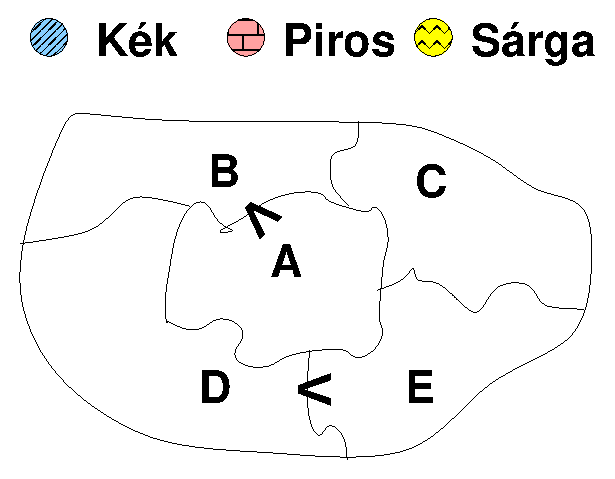
\epsfig{file=terkep.eps,width=0.2\textwidth}\end{center}

Elõször írjuk fel a megfelelõ korlátokat leíró \clpfd célsorozatot:

\begin{alltt}
| ?- use_module(library(clpfd)).
...
| ?- domain([A,B,C,D,E], 1, 3), 
     A #> B, A #\bs= C, A #\bs= D, A #\bs= E,
     B #\bs= C, B #\bs= D, C #\bs= E, D #< E.
A in 2..3, B in 1..2, C in 1..3, D in 1..2, E in 2..3 ? ;
no
\end{alltt}

Látható, hogy a Prolog az élkonzisztencia biztosítását elvégezte, de a
megoldást még nem tudta kikövetkeztetni. A megoldások meghatározásához
meg kell kérni a rendszert, hogy az \cd{A} változót rendre helyettesítse
be az 1, 2, 3 értékekre. Ez többféleképpen is elvégezhetõ: egyrészt a
hagyományos \cd{member/2} eljárással, amelynél azonban egyesével fel kell
sorolnunk \cd{A} lehetséges értékeit, ami nagy értékkészletnél kényelmetlen
lehet:

\begin{alltt}
| ?- domain([A,B,C,D,E], 1, 3), 
     A #> B, A #\bs= C, A #\bs= D, A #\bs= E,
     B #\bs= C, B #\bs= D, C #\bs= E, D #< E,
     member(A, [1,2,3]).
A = 3, B = 2, C = 1, D = 1, E = 2 ?
\end{alltt}

Az ilyen problémák megoldására szolgál az \cd{indomain/1} eljárás, amely
ezt a behelyettesítést automatikusan elvégzi a paraméterként adott változóra:

\begin{alltt}
| ?- domain([A,B,C,D,E], 1, 3), \ldots, indomain(A).
A = 3, B = 2, C = 1, D = 1, E = 2 ?
\end{alltt}

Elõfordulhatott volna azonban, hogy \cd{A} behelyettesítése még mindig
nem elég ahhoz, hogy kiderüljön az összes megoldás, ezért célszerû
a behelyettesítést mind az 5 változóra elvégezni. Ezt a \cd{labeling/2}
eljárás végzi, amely elsõ paramétere egy opciólista, amely a címkézés
menetét szabályozza (ezzel majd késõbb foglalkozunk), második paramétere
pedig egy változólista, amelyre a címkézést el akarjuk végezni.

\begin{alltt}
| ?- domain([A,B,C,D,E], 1, 3), \ldots, labeling([],[A,B,C,D,E]).
A = 3, B = 2, C = 1, D = 1, E = 2 ?
\end{alltt}

Annak megfogalmazására, hogy az \cd{A}, \cd{C} és \cd{E} változók értéke
mind különbözik, a Prolog kínál egy egyszerûbb és hatékonyabb megoldást is,
az \cd{all_distinct/1} predikátumot. Ez egy listát vár paraméterként, és
ügyel arra, hogy a lista összes eleme különbözõ értékeket vegyen fel.

\begin{alltt}
| ?- domain([A,B,C,D,E], 1, 3),
     A #> B, A #\bs= E, B #\bs= C, B #\bs= D, D #< E,
     all_distinct([A,C,E]). 
A = 3, B = 2, C = 1, D = 1, E = 2 ? ; no
\end{alltt}

Látható, hogy itt már címkézésre se volt szükség, mivel az \cd{all_distinct}
korlát ,,erõsebb'' a páronkénti különbözõségnél.

\subsubsection{Kódaritmetika (SEND+MORE=MONEY)}

\label{sendmoremoney}

A feladvány: írjon a betûk helyébe tízes számrendszerbeli számjegyeket
(azonosak helyébe azonosakat, különbözõek helyébe különbözõeket) úgy, hogy a
SEND+MORE=MONEY egyenlõség igaz legyen. Szám elején nem lehet 0 számjegy.

\begin{verbatim}
send(SEND, MORE, MONEY) :-
  length(List, 8),
  domain(List, 0, 9),               % tartományok 
  send(List, SEND, MORE, MONEY),    % korlátok
  labeling([], List).               % címkézés
\end{verbatim}
\begin{verbatim}
send(List, SEND, MORE, MONEY) :-
  List=[S,E,N,D,M,O,R,Y], 
  alldiff(List), S #\= 0, M #\= 0,
  SEND #=  1000*S+100*E+10*N+D,
  MORE #= 1000*M+100*O+10*R+E,
  MONEY #= 10000*M+1000*O+100*N+10*E+Y,
  SEND+MORE #= MONEY.
\end{verbatim}
\begin{alltt}
% alldiff(L): L elemei mind különbözõek (buta megvalósítás).
% Lényegében azonos a beépített all_different/1 kombinatorikai globális korláttal.
alldiff([]).
alldiff([X|Xs]) :- outof(X, Xs), alldiff(Xs).
\end{alltt}
\begin{verbatim}
outof(_, []).
outof(X, [Y|Ys]) :- X #\= Y, outof(X, Ys).
\end{verbatim}

A fenti programon jól látszik a szokásos \clpfd struktúra (tartományok
felvétele, korlátok felvétele, címkézés). Az ,,azonos betûk azonos számokat,
különbözõ betûk különbözõ számokat jelentenek'' kitételt egy saját
\cd{alldiff/1} predikátummal valósítjuk meg, amely lényegében megegyezik
az \cd{all_different/1} beépített globális korláttal. Fontos megjegyezni,
hogy az \cd{all_different/1} és az \cd{all_distinct/1} korlátok \emph{nem}
ekvivalensek, az elõbbi csak páronkénti különbözõséget valósít meg! Gyakran
azonban ez is elég, és az \cd{all_different} emellett gyorsabb futást biztosít,
tehát néha érdemes használni. Ezen magyarázat után lássuk a program futását:

\begin{verbatim}
| ?- send(SEND, MORE, MONEY).
MORE = 1085, SEND = 9567, MONEY = 10652 ? ;
no
\end{verbatim}

Nézzük meg azt is, hogy mit adna ki a program, ha elhagynánk a címkézést:

\begin{verbatim}
| ?- List=[S,E,N,D,M,O,R,Y], domain(List, 0, 9), 
     send(List, SEND, MORE, MONEY).
        List = [9,E,N,D,1,0,R,Y],
        SEND in 9222..9866,
        MORE in 1022..1088,
        MONEY in 10244..10888,
        E in 2..8, N in 2..8, D in 2..8, 
        R in 2..8, Y in 2..8 ? ; no
\end{verbatim}

Amint látható, a rendszer helybõl rájött arra, hogy mivel az eredmény öt
számjegybõl áll, a két összeadandó viszont csak négybõl, ezért \cd{M}
csak 1 lehet. Ha viszont \cd{M} 1, akkor \cd{S}-nek 9-nek kell lennie,
különben nem keletkezhet átvitel, ilyenkor viszont \cd{O} csak nulla lehet.
A többi változó értéke csak a címkézés után derül ki.

\subsubsection{A zebra feladat}
Szintén egy \Clpfd -ben könnyen megfogható feladat: adott 5 különbözõ
nemzetiségû ember, 5 különbözõ színû ház, 5 különbözõ foglalkozás, 5
különbözõ állat és 5 különbözõ ital. Egy embernek pontosan egy
foglalkozása, nemzetisége, háza, kedvenc itala és állata van. A
feladat az, hogy az ismert kötöttségek alapján megmondjuk, hogy melyik
nemzetiségû ember kedvenc állata a zebra. Az embereket megsorszámozzuk
1-tõl 5-ig, majd minden egyes foglalkozáshoz, nemzetiséghez, házhoz,
italhoz és állathoz egy constraint változót rendelünk, amely értékét
az 1..5 halmazból veszi fel. Egy ilyen változó $i$ értéke azt jelenti,
hogy az általa reprezentált tulajdonság az $i$. számú emberhez
tartozik. A kötöttségeket ez alapján könnyen felírhatjuk, például az,
hogy a diplomata háza a sárga, egyszerûen a két megfelelõ
constraint-változó egyenlõvé tételével biztosítható.  A kötöttségek a
programból könnyen kideríthetõk, itt nem soroljuk fel õket. Az
egyetlen figyelmet érdemlõ feltétel annak a megvalósítása, hogy
valaki egy adott ház szomszédjában lakik. Ezt a \cd{nextto/2} predikátum
kezeli. A \cd{nextto/2} tulajdonképpen egy vagylagos szerkezet, amit a
Prolog választási pontokkal valósít meg - vagyis spekulatív módon veszi fel a
vagy-kapcsolatban szereplõ korlátokat, és minden lehetõségre
megpróbálja megoldani az aktuális korlát rendszert. Ez nem a legszerencsésebb
megoldás, mivel sok választási pont esetén rengeteg idõt igényelhet. A
vagylagos szerkezetekrõl a \clpfd esettanulmányokban (\pageref{diszjunkcio}.
oldal) még lesz szó. Adott esetben a 

\begin{verbatim}
nextto(A,B):- abs(A-B) #= 1.
\end{verbatim}

megoldás sokkal szerencsésebb lenne, mivel ez nem generál választási
pontokat.

\begin{verbatim}
:- use_module(library(lists)).
:- use_module(library(clpfd)).

zebra(ZOwner, All):-
  All = [England,Spain,Japan,Norway,Italy,
         Green,Red,Yellow,Blue,White,
         Painter,Diplomat,Violinist,Doctor,Sculptor,
         Dog,Zebra,Fox,Snail,Horse,
         Juice,Water,Tea,Coffee,Milk],
  domain(All, 1, 5),
  alldiff([England,Spain,Japan,Norway,Italy]),
  alldiff([Green,Red,Yellow,Blue,White]),
  alldiff([Painter,Diplomat,Violinist,Doctor,Sculptor]),
  alldiff([Dog,Zebra,Fox,Snail,Horse]),
  alldiff([Juice,Water,Tea,Coffee,Milk]),
  England = Red,          Spain = Dog,
  Japan = Painter,        Italy = Tea,
  Norway = 1,             Green = Coffee,
  Green #= White+1,       Sculptor = Snail,
  Diplomat = Yellow,      Milk = 3,
  Violinist = Juice,      nextto(Norway, Blue),
  nextto(Fox, Doctor),    nextto(Horse, Diplomat),
  labeling([ff], All),
  nth(N, [England,Spain,Japan,Norway,Italy], Zebra),
  nth(N, [england,spain,japan,norway,italy], ZOwner).

nextto(A, B) :-  A #= B+1.
nextto(A, B) :-  A #= B-1.
\end{verbatim}

\subsubsection{N királynõ a sakktáblán}

A feladat elhelyezni egy $n * n$-es sakktáblán $n$ királynõt úgy, hogy
egyik se üsse a másikat.
\br
A megoldás minden királynõt külön oszlopba tesz, majd mindegyikükhöz
egy változót rendel, ami a királynõ oszlopbeli pozícióját adja meg. A
változók tartományának deklarálása után minden két királynõ között
felállít egy constraint-et (\cd{no\_threat/3}), ami azt adja meg, hogy
a két királynõ nem üti egymást. Ehhez meg kell adni a két királynõ
oszlopainak távolságát, ami itt az \cd{I} paraméter. Ezek után a
program végrehajtja a címkézést first-fail heurisztikával. A first-fail
elv mindig a legkisebb értékkészlettel rendelkezõ változót helyettesíti
be elõször, abban reménykedve, hogy így hamarabb kiderülnek a hibás ágak.
A címkézési módokról késõbb lesz szó.

\label{no:threat}

\begin{verbatim}
:- use_module(library(clpfd)).

% A Qs lista N királynõ biztonságos elhelyezését
% mutatja egy N*N-es sakktáblán. Ha a lista
% i. eleme j, akkor az i. királynõt az i. sor j.
% oszlopába kell helyezni.
queens(N, Qs):-
  length(Qs, N), domain(Qs, 1, N),
  safe(Qs),
  labeling([ff],Qs).  % first-fail elv

% safe(Qs): A Qs lista a királynõk biztonságos
% elhelyezését írja le.
safe([]).
safe([Q|Qs]):-
  no_attack(Qs, Q, 1),
  safe(Qs).

% no_attack(Qs, Q, I): A Qs lista által leírt
% királynõk egyike sem támadja a Q oszlopban levõ
% kiralynõt, feltéve hogy Q és Qs távolsága I.
no_attack([],_,_).
no_attack([X|Xs], Y, I):-
  no_threat(X, Y, I),
  J is I+1, no_attack(Xs, Y, J).

% Az X és Y oszlopokban  I sortávolságra levõ
% királynõk nem támadják egymást.
no_threat(X, Y, I) :-
  Y #= X, Y #= X-I, Y #= X+I.
\end{verbatim}



\subsection{Szûkítési szintek}
\label{szukites}

A könnyebb megértés érdekében elõször informálisan, egy egyszerû
kétargumentumú relációra fogjuk megfogalmazni az \emph{intervallum-szûkítés}
és a \emph{tartományszûkítés} fogalmát, utána pedig formalizáljuk a
leírtakat.
\br
Tekintsünk egy $r(X,Y)$ bináris relációt! Ekkor $r$ \emph{tartományszûkítése}
során $X$ tartományából elhagyjuk az összes olyan $x$ értéket, amelyhez nem
található $Y$ tartományában olyan $y$ érték, hogy $r(x,y)$ fennáll. Hasonlóan
szûkítjük $Y$ tartományát is. A folyamat eredménye az élkonzisztencia (lásd
a fogalom definícióját a \ref{cspfogalmak} fejezetben).
\emph{Intervallum-szûkítés} során viszont $X$ tartományából elhagyjuk annak
alsó vagy felsõ határát, ha ahhoz nem található olyan $y$ érték, amely $Y$
határai közé esik, és azzal az $r$ reláció fennáll. Hasonlóan szûkítjük
$Y$ tartományának határait is, és ezeket a lépéseket addig ismételjük,
amíg tudunk szûkíteni. Ez a módszer nem biztosít élkonzisztenciát, de
gyorsabban elvégezhetõ.
\br
Példa: legyen $x \in \{0,1,2,3,4,5\}$ és $y \in \{-1,1,3,4\}$, $r(x,y)$ pedig
az $x=|y|$ reláció. A tartományszûkítés $x$ értékkészletébõl elhagyja
a 0, 2, 5 értékeket, hiszen semelyik $y$ érték abszolútértéke nem lehet
sem 0, sem 2, sem 5. Az intervallum-szûkítés viszont elõször csak a 0
és az 5 kizárásával próbálkozik. 0-t nem zárhatja ki, hiszen $y$ tartományának
szélsõ értékei közé (tehát -1 és 4 közé) esik a 0, és $0=|0|$. 5-öt
kizárhatja, mert sem a -5, sem az 5 nem esik $y$ szélsõ értékei közé,
de a 4-et már nem zárhatja ki, ezért $x$ csak a $\{0,1,2,3,4\}$ halmazra
szûkül.
\br
A fenti példán jól látszik az intervallum-szûkítés két gyengesége:

\begin{enumerate}
\item csak a tartomány szélsõ értékeit hajlandó elhagyni, ezért nem hagyja el
a \cd{2} értéket;
\item a másik változó tartományában nem veszi figyelembe a ,,lyukakat'', így
a példában \cd{Y} tartománya helyett annak \emph{lefedõ intervallumát}, azaz
a \cd{-1..4} intervallumot tekinti, ezért nem hagyja el \cd{X}-bõl
a \cd{0} értéket.
\end{enumerate}

Ugyanakkor az intervallum-szûkítés általában konstans idejû mûvelet,
míg a tartományszûkítés ideje (és az eredmény mérete) erõsen függ a
tartományok méretétõl, ezért sok esetben a SICStus \clpfd könyvtár csak
az intervallum-szûkítést garantálja, a tartományszûkítést nem.
\br
Ezek után fogalmazzuk meg a definícióinkat formálisan is!

\enum{Jelölések}{
\item Legyen $C$ egy $n$-változós korlát, $s$ egy korlát-tár,
\item $D(X,s)$ az $X$ változó tartománya az $s$ tárban,
\item $D'(X,s) = {\rm min} D(X,s) .. {\rm max} D(X,s)$ az $X$ változó
      tartományát \emph{lefedõ} (legszûkebb) \emph{intervallum}.}

\enum{A szûkítési szintek definíciója}{
\item tartományszûkítés (domain consistency) \\
\definicio $C$ \emph{tartományszûkítõ}, ha minden szûkítési lépés lefutása után az
adott $C$ korlát él-konzisztens, azaz bármelyik $X_i$ változójához és annak
tetszõleges $V_i \in D(X_i,s)$ megengedett értékéhez található a többi
változónak olyan $V_j \in D(X_j,s)$ értéke ($j = 1, \ldots, i-1,i+1,\ldots, n$),
hogy $C(V_1, \ldots V_n)$ fennálljon. 
 
\item intervallum-szûkítés (interval consistency) \\
\definicio $C$ \emph{intervallum-szûkítõ} ha minden szûkítési lépés lefutása után igaz,
hogy $C$ bármelyik $X_i$ változója esetén e változó tartományának mindkét
{\em vég}pontjához (azaz a $V_i = {\rm min} D(X_i,s)$ illetve
$V_i = {\rm max} D(X_i,s)$ értékekhez) található a többi változónak
olyan $V_j \in D'(X_j,s)$ értéke ($j = 1, \ldots, i-1,i+1, \ldots, n$), hogy
$C(V_1, \ldots V_n)$ fennálljon.
}

A tartományszûkítés lokálisan (egy korlátra nézve) a lehetõ legjobb, de
nem garantálja a megoldást akkor sem, ha az összes korlát tartományszûkítõ,
mivel nem tudja figyelembe venni a többi korlát hatását. Ezt illusztrálja
a már bemutatott \cd{all_different $\longleftrightarrow$ all_distinct} probléma, ahol
kihasználjuk, hogy az \cd{all_different} ekvivalens a páronkénti különbözõségek
felvételével:

\begin{verbatim}
| ?- domain([X,Y,Z], 1, 2), X #\= Y, Y #\= Z, Z #\= X.
X in 1..2, Y in 1..2, Z in 1..2 ? ;
no
| ?- domain([X,Y,Z], 1, 2), all_distinct([X,Y,Z]).
no
\end{verbatim}

A SICStusban a halmazkorlátok (triviálisan) tartományszûkítõk. A
\emph{lineáris} aritmetikai korlátok legalább intervallum-szûkítõk,
a nemlineáris aritmetikai korlátokra nincs garantált szûkítési szint.
Ha a változók valamelyik határa végtelen (\cd{inf} vagy \cd{sup}), akkor
nincs garantált szûkítési szint, de az aritmetikai és a halmazkorlátok
ilyenkor is szûkítenek. A késõbb tárgyalt korlátokra egyenként megadjuk majd
a szûkítési szinteket.
\br
Néhány példa a szûkítési szintekre:
\begin{verbatim}
| ?- X in {4,9}, Y in {2,3}, Z #= X-Y. % intervallum-szûkítõ
X in {4}\/{9}, Y in 2..3, Z in 1..7 ? 
\end{verbatim}
\begin{verbatim}
| ?- X in {4,9}, Y in {2,3}, plus(Y, Z, X).
    % plus(A, B, C): A+B=C tartományszûkítõ módon
X in {4}\/{9}, Y in 2..3, Z in(1..2)\/(6..7) ? 
\end{verbatim}
\begin{verbatim}
| ?- X in {4,9}, Y in {2}, /* azaz Y=2 */, Z #= X-Y. % tartományszûkítõ
Y = 2, X in {4}\/{9}, Z in {2}\/{7} ? 
\end{verbatim}
\begin{verbatim}
| ?- X in {4,9}, Z #= X-Y, Y=2.
    % így csak intervallum-szûkítõ!
    % vö. fordítási idejû korlát-kifejtés
Y = 2, X in {4}\/{9}, Z in 2..7 ? 
\end{verbatim}
\begin{verbatim}
| ?-domain([X,Y], -10, 10), X*X+2*X+1 #= Y.
    % Ez nem intervallum-szûkítõ, Y<0 nem lehet!
X in -4..4, Y in -7..10 ? 
\end{verbatim}
\begin{verbatim}
| ?- domain([X,Y], -10, 10), (X+1)*(X+1) #= Y.
    % garantáltan nem, de intervallum-szûkítõ:
X in -4..2, Y in 0..9 ?   
\end{verbatim}



\subsection{Korlátok végrehajtása}

\label{korlatvegrehajtas}

Egy korlát végrehajtása több fázisból áll:

\begin{enumerate}
\item A korlát kifejtése belsõ, elemi korlátokra (ld. \ref{korlatkif}. fejezetben)
\item A korlát felvétele. Itt rögtön két lehetõség adódik:

	\begin{itemize}
	\item Egyszerû korlát (pl. \cd{X \#< 4}) esetén a korlát azonnal végrehajtásra kerül
	\item Összetett korlát esetén a korlátból démon képzõdik, a démon elvégzi a
	lehetséges szûkítéseit, meghatározza, hogy milyen feltételek esetén kell újra
	aktiválódnia, majd elalszik.
	\end{itemize}

\item Ha a korlátból démon képzõdött, és a démon ébresztési feltételei teljesülnek, akkor
aktiválódik, elvégzi a szûkítéseit, majd dönt a folytatásról. A döntés eredménye kétféle
lehet:

	\begin{itemize}
	\item Ha a démon már levezethetõ a tárból, akkor befejezi mûködését
	\item Ha a démon még nem vezethetõ le a tárból, akkor újból elalszik
	\end{itemize}

\end{enumerate}

Nézzük az eddig elmondottakat néhány konkrét példán!

\enumhead{\cd{A \#\bs= B} {\rm (tartományszûkítõ)}}
\begin{itemize}
\item {\bf Aktiválás feltétele:} ha \cd{A} vagy \cd{B} konkrét értéket kap
\item {\bf A szûkítés módja:} az adott értéket kizárja a másik változó értelmezési
tartományából
\item {\bf A folytatás menete:} mivel ilyenkor már a démon biztosan levezethetõ
a tárból, ezért a démon mûködése befejezõdik
\end{itemize}

\enumhead{\cd{A \#< B} {\rm (tartományszûkítõ)}}
\begin{itemize}
\item {\bf Aktiválás feltétele:} ha \cd{A} alsó határa (min(\cd{A})) vagy \cd{B}
felsõ határa (max(\cd{B})) változik
\item {\bf A szûkítés módja:} \cd{A} tartományából kihagyja az $X \ge$ max(\cd{B})
értékeket, \cd{B} tartományából pedig kihagyja az $Y \le$ min(\cd{A}) értékeket
\item {\bf A folytatás menete:} ha max(\cd{A}) $<$ min(\cd{B}), akkor lefut,
egyébként elalszik
\end{itemize}

\enumhead{\cd{all\_distinct([A$_1$,A$_2$,\ldots])} {\rm (tartományszûkítõ)}}
\begin{itemize}
\item {\bf Aktiválás feltétele}: ha bármelyik változó tartománya változik
\item {\bf A szûkítés módja}: páros gráfokban maximális párosítást keresõ
algoritmus segítségével minden olyan értéket elhagy, amelyek esetén a korlát nem
állhat fenn. Példa:
\begin{verbatim}
| ?- A in 2..3, B in 2..3, C in 1..3, 
     all_distinct([A,B,C]).
\end{verbatim}
\begin{verbatim}
                 C = 1, A in 2..3, B in 2..3 ? 
\end{verbatim}
\item {\bf A folytatás menete}: ha már csak egy nem-konstans argumentuma van,
akkor lefut, különben újra elalszik. Látszólag jobb döntésnek tûnhet, ha a korlát
akkor futna le, amikor a tartományok már mind diszjunktak, de a SICStus nem így
csinálja, valószínûleg azért, mert nem éri meg.
\end{itemize}

\enumhead{\cd{X+Y \#= T} {\rm (intervallum-szûkítõ)}}
\begin{itemize}
\item {\bf Aktiválás feltétele}: ha bármelyik változó alsó vagy felsõ határa változik (az
intervallum-szûkítés miatt nem minden tartományváltozásra ébred fel)
\item {\bf A szûkítés módja}: \cd{T}-t szûkíti a \cd{({\rm min} X+{\rm min} Y)..({\rm max}
X+{\rm max} Y)} intervallumra, \cd{X}-t szûkiti a \cd{({\rm min} T-{\rm max} 
Y)..({\rm max} T-{\rm min} Y)} intervallumra, \cd{Y}-t analóg módon szûkíti.
\item {\bf A folytatás menete}: ha (a szûkítés után) mindhárom változó konstans, akkor lefut,
különben újra elalszik.
\end{itemize}

Mivel a \clpfd alapvetõen ,,lusta'' mûködésû, és nem végez el minden lehetséges
szûkítést, ezért elõfordulhat, hogy ugyanazon változókra megfogalmazott, jelentéstartalomban
megegyezõ, de különbözõ szintaktikájú korlátok nem azonos mértékben szûkítenek,
mint ahogy azt a következõ példa is mutatja:

\begin{verbatim}
| ?- domain([X,Y], 0, 100), X+Y #=10, X-Y #=2.
                X in 2..10, Y in 0..8 ? 

| ?- domain([X,Y], 0, 100), X+Y #=10, X+2*Y #=14.
                X = 6, Y = 4 ? 
\end{verbatim}

Az alsó és a felsõ példának ugyanaz a megoldása, az elsõ esetben az \cd{X-Y \#= 2}
korlát intervallum-szûkítõ, és az intervallum-szûkítés a már fennálló \cd{X in 2..10}
és \cd{Y in 0..8} tartományokat nem tudja tovább szûkíteni. Az \cd{X+2*Y \#= 14}
korlát viszont ugyan garantáltan nem tartományszûkítõ, de itt mégis elvégzi a
tartományszûkítést, és ezzel megtalálja a megoldást.

\subsection{Korlátok tükrözése: \emph{reifikáció}}

\definicio egy $C$ korlát \emph{reifikáció}ja (\emph{tükrözés}e) a korlát
igazságértékének megjelenítése egy 0-1 értékû korlát változóban. Jelölése:
$C$ \cd{\#<=> B}. Ezt úgy kell értelmezni, hogy \cd{B} egy 0-1 értékû változó,
és \cd{B} akkor és csak akkor 1, ha $C$ igaz.
\br
{\bf Példa:} \cd{(X \#>= 3) \#<=> B} jelentése: \cd{B} az \cd{X $\ge$ 3} egyenlõtlenség
igazságértéke.
\br
Az eddig ismertetett halmaz- és aritmetikai korlátok (az úgynevezett \emph{formulakorlátok})
mind tükrözhetõek, de a globális korlátok (pl. \cd{all_different/1}, \cd{all_distinct/1})
nem. A \ref{fdpred}. fejezetben ismertetésre kerülõ FD predikátumok a
felhasználó határozza meg az FD predikátum klózainak megfelelõ kialakításával.
\br
Egy $C$ \cd{\#<=> B} korlát végrehajtása többféle szûkítést is igényel:

\begin{description}
\item a) amikor \cd{B}-rõl kiderül valami (azaz behelyettesítõdik): ha \cd{B=1},
fel kell venni ({\em post}) a korlátot, ha \cd{B=0}, fel kell venni a negáltját.
\item b) amikor $C$-rõl kiderül, hogy levezethetõ a tárból, végre kell hajtani
a \cd{B=1} helyettesítést
\item c) amikor $\lnot C$-rõl kiderül, hogy levezethetõ a tárból, végre kell
hajtani a \cd{B=0} helyettesítést
\end{description}

A fenti három fajta szûkítést három különbözõ démon végzi. A levezethetõségi vizsgálat
különbözõ ,,ambíciókkal'', különbözõ bonyolultsági szinteken végezhetõ el (bõvebben:
\ref{levezethetoseg}. fejezet).
\br
Lássuk a fent leírtakat mûködés közben!

\begin{itemize}
\item Alappélda, csak \cd{B} szûkül:
\begin{alltt}
| ?- X#>3 #<=> B.                  \(\Rightarrow\) B in 0..1
\end{alltt}
\item Ha \cd{B} értéket kap, akkor a rendszer felveszi a korlátot, illetve a negáltját:
\begin{alltt}
| ?- X#>3 #<=> B, B = 1.           \(\Rightarrow\) X in 4..sup
| ?- X#>3 #<=> B, B = 0.           \(\Rightarrow\) X in inf..3
\end{alltt}
\item Ha levezethetõ a korlát, vagy a negáltja, akkor \cd{B} értéket kap.
\begin{alltt}
| ?- X#>3 #<=> B, X in 15..sup.    \(\Rightarrow\) B = 1
| ?- X#>3 #<=> B, X in inf..0.     \(\Rightarrow\) B = 0
\end{alltt}
\item Ha a tár megengedi a korlát és a negáltja teljesülését is, akkor \cd{B} nem
kap értéket.
\begin{alltt}
| ?- X#>3 #<=> B, X in 3..4.       \(\Rightarrow\) B in 0..1
\end{alltt}
\item A rendszer kikövetkezteti, hogy az adott tárban \cd{X} és \cd{Y} távolsága legalább \cd{1}:
\begin{alltt}
| ?- abs(X-Y)#>1 #<=> B, X in 1..4, Y in 6..10.
             \(\Rightarrow\) B = 1
\end{alltt}
\item Bár a távolság-feltétel itt is fennáll, a rendszer nem veszi észre!
\begin{alltt}
| ?- abs(X-Y)#>1 #<=> B, X in \{1,5\}, Y in \{3,7\}.
             \(\Rightarrow\) B in 0..1 
\end{alltt}
\item Ennek itt az az oka, hogy az aritmetika nem tartomány-konzisztens.
\begin{alltt}
| ?- D #= X-Y, 
     AD #= abs(D), AD#>1 #<=> B, 
     X in \{1,5\}, Y in \{3,7\}.
             \(\Rightarrow\) D in -6..2, AD in 0..6, B in 0..1
\end{alltt}
\begin{alltt}
| ?- plus(Y, D, X),      \(\Leftarrow\){\rm tartomány-konzisztens összegkorlát}
     AD #= abs(D), AD#>1 #<=> B, 
     X in \{1,5\}, Y in \{3,7\}.
             \(\Rightarrow\) D in \{-6,-2,2\}, AD in \{2,6\}, B = 1
\end{alltt}
\end{itemize}

\subsection{Levezethetõségi szintek}

\label{levezethetoseg}

A SICStus Prolog kétfajta levezethetõségi szintet ismer, a tartományszûkítés
és az intervallum-szûkítés fogalmához hasonlóan:
\br
\definicio a $C$ $n$-változós korlát \emph{tartomány-levezethetõ} az $s$ tárból,
ha változóinak $s$-ben megengedett tetszõleges $V_j \in D(X_j,s)$ értékkombinációjára
($j = 1, \ldots, n$) $C(V_1, \ldots V_n)$ fennáll.
\br
\definicio a $C$ $n$-változós korlát \emph{intervallum-levezethetõ} az $s$ tárból,
ha változóinak $s$-ben megengedett tetszõleges $V_j \in D'(X_j,s)$ értékkombinációjára
($j = 1, \ldots, n$) $C(V_1, \ldots V_n)$ fennáll.
\br
A fentiekbõl a $D(x_j,s) \subseteq D'(x_j,s)$ relációt figyelembe véve következik, hogy
ha $C$ intervallum-levezethetõ, akkor tartomány-levezethetõ is. A kétféle levezethetõségi
vizsgálatra azért van szükség, mert a tartomány-levezethetõség vizsgálata általában
bonyolultabb (és tovább is tart), mint az intervallum-levezethetõségé. Például az
\cd{X \#\bs= Y} korlát tartomány-levezethetõ, ha \cd{X} és \cd{Y} tartományai
diszjunktak (a tartományok méretével arányos költség), ugyanakkor az
intervallum-levezethetõséghez elég az \cd{X} és \cd{Y} tartományainak lefedõ
intervallumait vizsgálni (ami konstans költségû mûvelet).
\br
A SICStus-ban a tükrözött halmazkorlátok kiderítik a tartomány-levezethetõséget, a
tükrözött \emph{lineáris} aritmetikai korlátok legalább az intervallum-levezethetõséget
(egyes esetekben a tartomány-levezethetõséget is, lásd az elõzõ alfejezet utolsó 4
példáját). A tükrözött nemlineáris aritmetikai korlátokra még az intervallum-levezethetõség
kiderítése sem garantálható.

\subsection{Egy bonyolultabb \clpfd példa: mágikus sorozatok}

\definicio egy $L = (x_{0}, x_{1}, \ldots, x_{n-1})$ sorozat \emph{mágikus}
($x_{i} \in [0..n-1]$), ha minden $i \in [0..n-1]$-re $L$-ben az $i$ szám pontosan
$x_{i}$-szer fordul elõ.
\br
{\bf Példa:} $n$=4 esetén (1,2,1,0) és (2,0,2,0) mágikus sorozatok.
\br
A feladat \clpfd megoldásához definiálni fogunk a sorozatok között egy transzformációt:
\br
\definicio az $X = (x_{0}, x_{1}, \ldots, x_{n-1})$ sorozatnak az
$Y = \mathcal{E}(X) = (y_{0}, y_{1}, \ldots, y_{n-1})$ sorozat az
\emph{elõfordulás-sorozat}a, ha minden $i \in [0..n-1]$-re $X$-ben az $i$ szám
pontosan $y_{i}$-szer fordul elõ.

\subsubsection{Egyszerû \clpfd megoldás}

Látható, hogy a mágikus sorozatok azok a sorozatok, amelyek erre a $\mathcal{E}$
transzformációra nézve fixpontok (azaz olyan sorozatok, amelyeket a transzformáció
önmagába visz át). Ennek felhasználásával a feladatra könnyen adható egy néhány
soros \clpfd megoldás:

\begin{alltt}
% Az L lista egy N hosszúságú mágikus sorozat.
magikus(N, L) :-
        length(L, N), N1 is N-1, domain(L, 0, N1),
        elofordulasok(L, 0, L),
        labeling([], L).             % most felesleges

% elofordulasok([E\(_\cd{i}\), E\(_\cd{i+1}\), \ldots], i, Sor): Sor-ban az i
% szám E\(_\cd{i}\)-szer, az i+1 szám E\(_\cd{i+1}\)-szer stb. fordul elõ.
% Ez a predikátum valósítja meg a fenti elõfordulás-sorozat transzformációt
elofordulasok([], _, _).
elofordulasok([E|Ek], I, Sor) :-
        pontosan(I, Sor, E), 
        J is I+1, elofordulasok(Ek, J, Sor).

% pontosan(I, L, E): Az I szám L-ben E-szer fordul elõ.
pontosan(I, L, 0) :- outof(I, L).
pontosan(I, [I|L], N) :- 
        N #> 0, N1 #= N-1, pontosan(I, L, N1).
pontosan(I, [X|L], N) :- 
        N #> 0, X #\bs= I, pontosan(I, L, N).

% outof(I, L): Az I szám L-ben nem fordul elõ.
outof(_, []).
outof(X, [Y|Ys]) :- X #\bs= Y, outof(X, Ys).
\end{alltt}

Példafutás (csak a \cd{pontosan/3} hívások érdekelnek minket):

\begin{verbatim}
| ?- spy pontosan/3, magikus(4, L).
 +      1      1 Call: pontosan(0,[_A,_B,_C,_D],_A) ? s
?+      1      1 Exit: pontosan(0,[1,0,_C,_D],1) ? z
 +      2      1 Call: pontosan(1,[1,0,_C,_D],0) ? s
 +      2      1 Fail: pontosan(1,[1,0,_C,_D],0) ? z
 +      1      1 Redo: pontosan(0,[1,0,_C,_D],1) ? s
?+      1      1 Exit: pontosan(0,[2,0,0,_D],2) ? z
(...)
 +      4      1 Call: pontosan(2,[2,0,0,_D],0) ? s
 +      4      1 Fail: pontosan(2,[2,0,0,_D],0) ? z
(...)
?+      1      1 Exit: pontosan(0,[3,0,0,0],3) ? z
(...)
?+      1      1 Exit: pontosan(0,[2,0,_D,0],2) ?
\end{verbatim}

\subsubsection{Redundáns korlátok bevezetése}

A fenti változat hatékonyságán sokat segíthetünk \emph{redundáns korlátok}
felvételével. A redundáns korlátok olyan korlátok, amelyek formálisan nem
közölnek új információt a feladatról, hanem a már fennálló korlátok következményei,
azonban úgy vannak ,,megfogalmazva'', hogy ezzel segítik a program végrehajtását,
mert olyan esetekben is szûkítéseket eredményeznek, amikor a redundancia nélküli
változat erre nem volt képes. A redundáns korlátokhoz a következõ állítást
fogjuk felhasználni:
\br
\tetel ha az $L = (x_{0}, x_{1}, \ldots, x_{n-1})$ sorozat mágikus,
akkor $\sum_{i<n} x_{i} = n$ és $\sum_{i<n} i \times x_{i} = n$.
\br
Ezzel a program fõ klóza a következõképpen módosul:
\begin{alltt}
% Az L lista egy N hosszú mágikus sorozat
magikus2(N, L) :-
    length(L, N), N1 is N-1, domain(L, 0, N1),
    osszege(L, S),               % \(\sum_{i\in [1..\cd{N}]} L_{i} = \cd{S}\)
    szorzatosszege(L, 0, SP),    % \(\sum_{i\in [1..\cd{N}]} i*L_{i} = \cd{SP}\)
    call(S #= N), call(SP #= N), % lásd a megjegyzést
    elofordulasok(L, 0, L).      % lásd az elõzõ lapon

% osszege(L, Ossz): Ossz = \(\sum_i \cd{L}_i\)
osszege([], 0).
osszege([X|L], X+S) :- osszege(L, S).

% szorzatosszege(L, I, Ossz): Ossz = \(\cd{I}*\cd{L}_1+\cd{(I+1)}*\cd{L}_2+\ldots\)
szorzatosszege([], _, 0).
szorzatosszege([X|L], I, I*X+S) :- 
    J is I+1, szorzatosszege(L, J, S).
\end{alltt}

Az \cd{osszege/2} és a \cd{szorzatosszege/3} hívásokat külön nem fejtjük ki, ezek
a megfelelõ korlát-kifejezéseket \emph{építik fel} az \cd{S} és \cd{SP} változókba.
A \cd{call/1} alkalmazására azért van szükség, mert a korlátokat a \clpfd könyvtár
fordítási idõben átalakítja a saját, belsõ formátumára, és ez a felhasználó által
futásidõben felépített korlátokra nem történik meg. A megoldást a korlátkifejtési
fázis késleltetése jelenti a \cd{call/1} segítségével. Egyébként a programnak ez a
változata \cd{N=10} esetben kb. ötvenszer gyorsabb az elõzõ verziónál, és a 4 hosszú
mágikus sorozatok közül az elsõ megoldást visszalépés nélkül adja ki!

\subsubsection{Tükrözéses megoldás}

A tükrözés mechanizmusának felhasználásával egy elegáns, ráadásul hatékonyabb
megfogalmazást is adhatunk a \cd{pontosan/3} eljárásra, és ezzel az egész
feladatra:

\begin{verbatim}
magikus3(N, L) :-
        length(L, N), 
        N1 is N-1, domain(L, 0, N1),
        osszege(L, S), call(S #= N), 
        szorzatosszege(L, 0, SS), call(SS #= N),
        elofordulasok3(L, 0, L),
        labeling([], L). % most már kell a címkézés!

% A korábbi elofordulasok/3 másolata
elofordulasok3([], _, _).
elofordulasok3([E|Ek], I, Sor) :-
        pontosan3(I, Sor, E), 
        J is I+1, elofordulasok3(Ek, J, Sor).

% pontosan3(I, L, E): L-ben az I E-szer fordul elõ.
pontosan3(_, [], 0).
pontosan3(I, [X|L], N) :-
        X #= I #<=> B, N #= N1+B, pontosan3(I, L, N1).
\end{verbatim}

A megoldás lényege, hogy a \cd{pontosan3/3} eljárásban az \cd{L} lista
minden \cd{X} elemére felveszünk egy \cd{X \#= I} korlátot, és ennek igazságértékét
egy \cd{B} változóban tükrözzük. Az összes \cd{B} érték összegének pontosan
\cd{E}-vel kell megegyeznie. Ezzel a megoldással sikerült kiszûrni a \cd{pontosan/3}
eljárásból az eddig meglévõ diszjunkciót, és ezzel sokkal hatékonyabb kódot
sikerült készítenünk, ami az alábbi összehasonlító táblázatból is látszik
(1 perc idõkorlát, Pentium III 600 MHz-es processzor):

\begin{center}
\begin{tabular}{|l|rrrrrr|}
\hline
variáns/adat                   & n=10  & n=20 & n=40  & n=80  & n=160 & n=320 \\
\hline                         
választós                      & 13.90 & ---  &  ---  &  ---  & ---  & ---    \\
választós+\cd{osszege}         &  0.22 & ---  &  ---  &  ---  & ---  & ---    \\
vál.+\cd{szorzatosszege}       &  0.02 & 0.55 & 44.04 &  ---  & ---  & ---    \\
vál.+\cd{ossz}+\cd{szorzossz}  &  0.02 & 0.29 & 17.98 &  ---  & ---  & ---    \\
tükrözéses                     &  0.05 & 1.07 & 24.02 &  ---  & ---  & ---    \\
tükrözéses+\cd{osszege}        &  0.01 & 0.14 &  1.71 & 20.15 & ---  & ---    \\
tükr.+\cd{szorzatosszege}      &  0.01 & 0.04 &  0.18 &  0.94 & 4.75 & 25.77  \\
tükr.+\cd{ossz}+\cd{szorzossz} &  0.01 & 0.05 &  0.19 &  0.95 & 4.61 & 23.57  \\
\hline
\end{tabular}
\end{center}

\subsection{Logikai korlátok}

Annak ellenére, hogy a \clpfd könyvtár alapvetõen véges, egész értékû tartományok 
kezelésére használatos, lehetõség van logikai korlátok használatára is. Logikai
korlátokat háromféle alkotóelembõl építhetünk fel:

\begin{itemize}
\item változókból, ilyenkor a változók tartománya automatikusan a 0..1 tartományra
szûkül (a 0 a logikai hamis, az 1 a logikai igaz értéket fogja jelenteni)
\item tükrözhetõ aritmetikai- vagy halmazkorlátokból
\item más logikai korlátokból
\end{itemize}

Ezen építõelemek összekapcsolására az alábbi operátorok használatosak:

\begin{center}\begin{tabular}{|l|l|l|}
\hline
\verb'#\ Q'     &           negáció\ \ \ \ \ & \verb'op(710,  fy, #\).'\\
\verb'P #/\ Q'  &           konjunkció       & \verb'op(720, yfx, #/\).'\\
\verb'P #\ Q'   &           kizáró vagy      & \verb'op(730, yfx, #\).'\\
\verb'P #\/ Q'  &           diszjunkció      & \verb'op(740, yfx, #\/).'\\
\verb'P #=> Q'  &           implikáció       & \verb'op(750, xfy, #=>).'\\
\verb'Q #<= P'  &           implikáció       & \verb'op(750, yfx, #<=).'\\
\verb'P #<=> Q' &           ekvivalencia     & \verb'op(760, yfx, #<=>).'\\
\hline
\end{tabular}\end{center}

Észrevehetjük, hogy a korlátok igazságértékének tükrözésére használt \cd{\#<=>}
operátor jelen van a fenti táblázatban is. Ennek az az oka, hogy a tükrözési
jelölés valójában a logikai korlát-fogalom speciális esete. Fontos azonban megjegyezni,
hogy az \emph{összes} logikai korlát a \cd{$C$ \#<=> B} alakú \emph{elemi}
korlátra vezetõdik vissza. Például:

\begin{center}
\cd{X \#= 4 \#\bs/ Y \#> 6 $\Longleftrightarrow$ X \#= 4 \#<=> B1, Y \#> 6 \#<=> B2, B1+B2 \#> 0}
\end{center}

{\bf Vigyázat!} A diszjunktív logikai korlátok gyengén szûkítenek: egy $n$-tagú
diszjunkció csak akkor tud szûkíteni, ha egy kivételével valamennyi tagjának a
negáltja levezethetõvé válik (a fenti példában akkor, ha \cd{X \#\= 4} vagy \cd{Y \#\=< 6}
levezethetõ lesz).

\subsection{Példa a logikai korlátokra: lovagok, lókötõk és normálisak}

Egy szigeten minden bennszülött lovag, lókötõ, vagy normális. A lovagok mindig
igazat mondanak, a lókötõk mindig hazudnak, a normális emberek pedig néha
hazudnak, néha igazat mondanak. Adott három bennszülött, $A$, $B$ és $C$, akik
közül egy lovag, egy lókötõ és egy normális (de nem feltétlenül ebben a sorrendben).
Az alábbi állításokat teszik:

\begin{center}\begin{tabular}{ccc}
$A$: Én normális vagyok. & $B$: $A$ igazat mond. & $C$: Én nem vagyok normális.
\end{tabular}\end{center}

Kérdés: melyikõjük lovag, melyikõjük lókötõ és melyikõjük normális?
\br
A \clpfd megoldás során alkalmazzuk az alábbi kódolást: normális $\to$ \cd{2},
lovag $\to$ \cd{1}, lókötõ $\to$ \cd{0} (ez azért jó, mert így minden lovag
állítása az 1-es igazságértékbe, és minden lókötõ állítása a 0-s igazságértékbe
tükrözhetõ, ami megegyezik a hozzájuk rendelt azonosítóval).

\begin{verbatim}
:- use_module(library(clpfd)).

% Bevezetünk néhány operátort az állítások egyszerûbb leírására.
:- op(700, fy, nem).     :- op(900, yfx, vagy).  
:- op(800, yfx, és).     :- op(950, xfy, mondja).

% A B bennszülött mondhatja az Áll állítást.
B mondja Áll :- értéke(B mondja Áll, 1).

% értéke(A, Érték): Az A állítás igazságértéke Érték.
értéke(X = Y, E) :-
    X in 0..2, Y in 0..2, E #<=> (X #= Y).
értéke(X mondja M, E) :-
    X in 0..2, értéke(M, E0), 
    E #<=> (X #= 2 #\/ E0 #= X).
értéke(M1 és M2, E) :-
    értéke(M1, E1), értéke(M2, E2), E #<=> E1 #/\ E2.
értéke(M1 vagy M2, E) :-
    értéke(M1, E1), értéke(M2, E2), E #<=> E1 #\/ E2.
értéke(nem M, E) :-
        értéke(M, E0), E #<=> #\E0.

| ?- all_different([A,B,C]), A mondja A = 2, 
     B mondja A = 2, C mondja nem C =2,
     labeling([], [A,B,C]).
A = 0, B = 2, C = 1 ? ;
no
\end{verbatim}

\subsection{További globális aritmetikai korlátok}

Az eddigiek során már megismerkedhettünk két globális korláttal: az \cd{all_different/1}
és az \cd{all_distinct/1} korlátokkal. A SICStus azonban ismer még néhány hasznos
globális aritmetikai korlátot is, amelyeket ebben a fejezetben fogunk bemutatni. Ezen
korlátok közös jellemzõje, hogy a többi globális korláthoz hasonlóan nem tükrözhetõek.

\begin{itemize}
\item \cd{scalar_product(Coeffs, Xs, RelOp, Value)} \\
Igaz, ha a \cd{Coeffs} egészekbõl álló együttható-lista és az \cd{Xs} korlát-változókból
és egészekbõl álló lista skalárszorzata a \cd{RelOp} relációban áll a \cd{Value}
értékkel (\cd{Value} lehet egész szám vagy korlát-változó). \cd{RelOp} egy tetszõleges
aritmetikai összehasonlító operátor (pl. \cd{\#=}, \cd{\#<} stb.). Intervallum-szûkítést
biztosít. Érdekességként megjegyezzük, hogy minden lineáris aritmetikai korlát
átalakítható egy megfelelõ \cd{scalar_product} hívássá.

\item \cd{sum(Xs, RelOp, Value)} \\
Igaz, ha az \cd{Xs} korlát-változókból és egészekbõl álló lista összege a \cd{RelOp}
relációban áll a \cd{Value} értékkel (\cd{Value} lehet egész szám vagy korlát-változó).
Megegyezik a \cd{scalar_product(Csupa1, Xs, RelOp, Value)} hívással, ahol \cd{Csupa1}
csupa 1-es számból álló lista, és a hossza megegyezik \cd{Xs} hosszúságával.

\item \cd{knapsack(Coeffs, Xs, Value)} \\
Jelentése: \cd{Coeffs} és \cd{Xs} skalárszorzata \cd{Value}. Csak nem-negatív
számok és véges tartományú változók megengedettek, viszont cserébe tartomány-konzisztenciát
biztosít.
\end{itemize}

A \ref{sendmoremoney}. fejezetben ismertetett kódaritmetika példa egyszerûbb megoldása
\cd{scalar_product/4} segítségével:

\begin{verbatim}
send(List, SEND, MORE, MONEY) :-
        List= [S,E,N,D,M,O,R,Y], 
        Pow10 = [1000,100,10,1],
        all_different(List), S #\= 0, M#\= 0,
        scalar_product(Pow10, [S,E,N,D], #=, SEND),
        %   SEND #=  1000*S+100*E+10*N+D,
        scalar_product(Pow10, [M,O,R,E], #=, MORE),
        %   MORE #= 1000*M+100*O+10*R+E,
        scalar_product([10000|Pow10], [M,O,N,E,Y], 
                       #=, MONEY),
        %   MONEY #= 10000*M+1000*O+100*N+10*E+Y,
        SEND+MORE #= MONEY.
\end{verbatim}

\subsection{A formulakorlátok belsõ megvalósítása}
\label{korlatkif}

\definicio \emph{formulakorlát}oknak nevezzük az összes operátoros
jelöléssel írt korlátot, tehát az eddig tárgyalt összes korlátot, a
globális korlátok kivételével.
\br
Mint azt már a \ref{korlatvegrehajtas}. fejezet elején említettük, a
formulakorlátokat a SICStus \clpfd könyvtára elemi korlátok konjunkciójára
fordítja le a \cd{goal_expansion/3} kampó-eljárás segítségével. Ez az
eljárás minden formulakorlátot fordítási idõben a \cd{scalar_product/4}
korlátra és/vagy nem publikus elemi korlátokra fejt ki. Az átfordítás
futásidõig elhalasztható a korlát \cd{call/1}-be való ágyazásával, ez
a futás közben felépített formulakorlátok esetén hasznos.

\enumhead{A legfontosabb elemi korlátok a \cd{clpfd} modulban}
\begin{itemize}
\item aritmetika:\verb?'x+y=t'/3 'x*y=z'/3 'x/y=z'/3 'x mod y=z'/3?
\verb?'|x|=y'/2 'max(x,y)=z'/3 'min(x,y)=z'/3?
 \item összehasonlítás: \verb?'x=y'/2, 'x=<y'/2, 'x\\=y'/2?
és tükrözött változataik: \cd{iff\_aux('x {\em Rel} y'(X,Y), B)},
ahol {\tt\em Rel} $\in$ \{ \verb?= =< \=?\} .
\item halmazkorlátok: \cd{propagate_interval(X,Min,Max)
prune_and_propagate(X,Halmaz)}
\item logikai korlátok: \cd{bool(Muvkod,X,Y,Z)} (jelentése: \cd{X Muv Y = Z})
\item optimalizálások: \cd{'x*x=y'/2 'ax=t'/3 'ax+y=t'/4 'ax+by=t'/5
't+u=<c'/3 't=u+c'/3 't=<u+c'/3 't\bs=u+c'/3 't>=c'/2} stb.
\end{itemize}

\label{pontszukites}
A legtöbb elemi korlát \emph{pontszûkítõ}. A pontszûkítés definíciója
a következõképpen hangzik: egy $C$ korlát \emph{pontszûkítõ}, ha minden
olyan tár esetén tartományszûkítõ, amelyben $C$ változói legfeljebb
egy kivétellel be vannak helyettesítve (másképpen: minden ilyen tár esetén
a korlát a behelyettesítetlen változót pontosan a $C$ reláció által
megengedett értékekre szûkíti). Az egyetlen, nem pontszûkítõ elemi
korlát a \cd{mod}.
\br
Lineáris korlátok esetén a kifejtés megõrzi a pont-, illetve az
intervallum-szûkítést, általános esetben azonban még a pont-szûkítést
sem õrzi meg, pl:

\begin{verbatim}
| ?- X in 0..10, X*X*X*X #= 16.
X in 1..4 ? ;
no
\end{verbatim}

A korlátkifejtés mechanizmusát a \cd{goal_expansion/4} segédeljárás
hívásával magunk is megvizsgálhatjuk:

\begin{verbatim}
| ?- use_module(library(clpfd)).
| ?- goal_expansion(X*X+2*X+1 #= Y, user, G).
        G = clpfd:('x*x=y'(X,_A),
            scalar_product([1,-2,-1],[Y,X,_A],#=,1)) ? 

| ?- goal_expansion((X+1)*(X+1) #= Y, user, G).
        G = clpfd:('t=u+c'(_A,X,1),'x*x=y'(_A,Y)) ? 

| ?- goal_expansion(abs(X-Y)#>1, user, G).
        G = clpfd:('x+y=t'(Y,_A,X),
               '|x|=y'(_A,_B),'t>=c'(_B,2)) ? 

| ?- goal_expansion(X#=4 #\/ Y#>6, user, G).
        G = clpfd:iff_aux(clpfd:'x=y'(X,4),_A),
               clpfd:iff_aux(clpfd:'x=<y'(7,Y),_B),
               clpfd:bool(3,_A,_B,1) ?  % 3 a \/ kódja

| ?- goal_expansion(X*X*X*X #= 16, user, G).
        G = clpfd:('x*x=y'(X,_A),'x*y=z'(_A,X,_B),
                      'x*y=z'(_B,X,16)) ? 

| ?- goal_expansion(X in {1,2}, user, G).
        G = clpfd:propagate_interval(X,1,2) ? 

| ?- goal_expansion(X in {1,2,5}, user, G).
        G = clpfd:prune_and_propagate(X,[[1|2],[5|5]]) ?
\end{verbatim}

\subsection{Segédeljárások a \Clpfd -ben}

\enumhead{Statisztika}
\begin{itemize}
\item {\tt fd\_statistics(Kulcs, Érték)}: A \cd{Kulcs}-hoz tartozó
        számláló értékét \cd{Érték}-ben kiadja, és a számlálót lenullázza.
        Lehetséges kulcsok és számlált események: 
\begin{itemize}
\item \cd{constraints} --- korlát létrehozása
\item \cd{resumptions} --- korlát felébresztése
\item \cd{entailments} --- korlát (vagy negáltja) levezethetõvé válásának
        észlelése
\item \cd{prunings}    --- tartomány szûkítése
\item \cd{backtracks}  --- a korlát-tár ellentmondásossá válása miatt
        bekövetkezõ visszalépés (tehát Prolog meghiúsulások nem számítanak).
\end{itemize}
\item \cd{fd\_statistics}: az összes számláló állását kiírja és
        lenullázza õket.
\end{itemize}

Példa:

\begin{alltt}
% Az N-királynõ feladat összes megoldása Ss, Lab címkézéssel való
% végrehajtása Time msec-ig tart és Btrks FD visszalépést igényel.
run_queens(Lab, N, Ss, Time, Btrks) :-
        fd_statistics(backtracks, _), statistics(runtime, _),
        findall(Q, queens(Lab, N, Q), Ss),
        statistics(runtime, [_,Time]),
        fd_statistics(backtracks, Btrks).
\end{alltt}

\enumhead{A még le nem futott, alvó korlátok kiírása a válaszban)}
\begin{itemize}
\item \cd{clpfd:full\_answer}: ez egy dinamikus kampó eljárás.
        Alaphelyzetben nincs egy klóza sem, tehát nem sikerül. Ez
        esetben a rendszer egy kérdésre való válaszoláskor csak a
        kérdésben elõforduló változók tartományát írja ki, az alvó
        korlátokat nem. Ha felveszünk egy ilyen eljárást és az sikeresen
        fut le, akkor a válaszban az összes változó mellett kiírja még a
        le nem futott összes korlátot is.  
\end{itemize}

\begin{alltt}
| ?- domain([X,Y], 1, 10), X+Y#=5. \(\Rightarrow\) X in 1..4, Y in 1..4 ? 
| ?- assert(clpfd:full_answer).    \(\Rightarrow\) yes
| ?- domain([X,Y], 1, 10), X+Y#=5. \(\Rightarrow\) clpfd:'t+u=c'(X,Y,5), 
                                      X in 1..4, Y in 1..4 ? 
| ?- X+Y #= Z #<=> B.              \(\Rightarrow\) clpfd:'t=u IND'(Z,_A)#<=>B,
                                      clpfd:'x+y=t'(X,Y,_A), B in 0..1, \ldots
| ?- retract(clpfd:full_answer).   \(\Rightarrow\) yes
| ?- X+Y #= Z #<=> B.              \(\Rightarrow\) B in 0..1, \ldots
\end{alltt}

\subsection{FD-változók és FD-halmazok}
\label{fdset}

\definicio \emph{FD-változó}nak nevezünk minden olyan Prolog változót,
amely a korlát-tár korlátaiban szerepel, és ezért a \clpfd könyvtár különbözõ
információkat tart fenn róla. Az FD-változókról tárolt információkat a
programban felhasználhatjuk, de nagy valószínûséggel csak a címkézésnél,
nyomkövetésnél, illetve globális korlátokban látjuk hasznukat.
\br
Az FD-változókkal kapcsolatban a következõ eljárásokat érdemes ismerni:

\begin{itemize}
\item \cd{fd\_var(V)}: \cd{V} egy, a \clpfd könyvtár által ismert változó.
\item \cd{fd\_min(X, Min)}: a \cd{Min} paramétert egyesíti az \cd{X}
változó tartományának alsó határával (ez egy szám vagy \cd{inf} lehet).
\item \cd{fd\_max(X, Max)}: a \cd{Max} paramétert egyesíti az \cd{X}
változó tartományának felsõ határával (ez egy szám vagy \cd{sup} lehet).
\item \cd{fd\_size(X, Size)}: \cd{Size} az \cd{X} tartományának számossága
(szám vagy \cd{sup}).
\item \cd{fd\_dom(X, Range)}: \cd{Range} az \cd{X} változó tartománya,
tartománykifejezés formában 
\item \cd{fd\_set(X, Set)}: \cd{Set} az \cd{X} tartománya úgynevezett
\emph{FD-halmaz} formában (ld. lejjebb).
\item \cd{fd\_degree(X, D)}: \cd{D} az \cd{X}-hez kapcsolódó korlátok
száma.
\end{itemize}

Néhány példa a fentiek használatával:

\begin{verbatim}
| ?- X in (1..5)\/{9}, fd_min(X, Min), fd_max(X, Max), fd_size(X, Size).
Min = 1, Max = 9, Size = 6, X in(1..5)\/{9} ? 
| ?- X in (1..9)/\ \(6..8), fd_dom(X, Dom), fd_set(X, Set).
Dom = (1..5)\/{9}, Set = [[1|5],[9|9]], X in ... ?
| ?- queens_nolab(8, [X|_]), fd_degree(X, Deg).
Deg = 21, X in 1..8 ?         % mivel 21 = 7*3
\end{verbatim}

A pár sorral elõbb említett \emph{FD-halmaz}ok a \clpfd könyvtárban a
tartományok belsõ ábrázolási formáját jelentik. Jelenleg egy FD-halmaz
\cd{[Alsó|Felsõ]} alakú szeparált zárt intervallumok rendezett listája (mivel
a \cd{.(_,_)} struktúra memóriaigénye 33\%-kal kisebb, mint bármely más
\cd{f(_,_)} struktúráé), ezt azonban \emph{szigorúan tilos} kihasználni, nem
szabad ilyen adatszerkezetet a rendelkezésre álló könyvtári eljárásokon
kívül más módszerrel létrehozni vagy megváltoztatni! Az ilyen jellegû
megoldások elõbb-utóbb \cd{segmentation violation} vagy hasonló jellegû
hibaüzenethez vezetnek.
\br
Az adattípus manipulálására szolgáló könyvtári eljárások:

\begin{itemize}
\item \cd{is\_fdset(S)}: \cd{S} egy korrekt FD-halmaz.
\item \cd{empty\_fdset(S)}: \cd{S} az üres FD-halmaz.
\item \cd{fdset\_singleton(S,E)}: \cd{S} egyedül az \cd{E} elemet tartalmazza.
\item \cd{fdset\_interval(Set, Min, Max)}: \cd{S} egyedül a \cd{Min..Max}
intervallum elemeit tartalmazza
\item \cd{empty\_interval(Min, Max)}: \cd{Min..Max} egy üres intervallum
(ekvivalens a \cd{\bs+ fdset\_interval(_, Min, Max)} hívással).
\item \cd{fdset\_parts(S, Min, Max, Rest)}: Az \cd{S} FD-halmaz áll egy
\cd{Min..Max} kezdõ intervallumból és egy \cd{Rest} maradék FD-halmazból, ahol
\cd{Rest} minden eleme nagyobb \cd{Max+1}-nél. Egyaránt használható
FD-halmaz szétszedésére és építésére.
\begin{verbatim}
| ?- X in (1..9) /\ \(6..8), fd_set(X, _S), 
     fdset_parts(_S, Min1, Max1, _).
         Min1 = 1, 
         Max1 = 5, 
         X in(1..5)\/{9} ? 
\end{verbatim}
\item \cd{fdset\_union(Set1, Set2, Union)}: \cd{Set1} és \cd{Set2}
uniója \cd{Union},  
\cd{fdset\_union(ListOfSets, Union)}: a \cd{ListOfSets} FD halmazokból
álló lista elemeinek uniója \cd{Union}.
\item \cd{fdset\_intersection/[3,2]} : Két halmaz, illetve egy listában
megadott halmazok metszete (analóg az \cd{fdset\_union/[3,2]}-vel)
\item \cd{fdset\_complement(Set1, Set2)}: \cd{Set1} és \cd{Set2} egymás
komplemensei
\item \cd{fdset\_member(Elt, Set)}: \cd{Elt} eleme a \cd{Set} FD-halmaznak.
Visszalépésre az összes elemet felsorolja
\item \cd{list_to_fdset(List, Set), fdset_to_list(Set, List)}: számlista
átalakítása FD-halmazzá, és fordítva.
\item \cd{range_to_fdset(Range, Set), fdset_to_range(Set, Range)}:
tartománykifejezés átalakítása FD-halmazzá és viszont.
\end{itemize}

Itt jegyeznénk meg, hogy egy FD-halmaz szintén felhasználható egy változó
tartományának szûkítésére az \cd{X in_set Set} hívás használatával, azonban
vegyük figyelembe, hogy ha \cd{Set}-et egy \cd{Y} változó tartományának
függvényében alakítjuk ki, akkor ezzel még nem érünk el ,,démoni'' hatást,
mivel a szûkítés csak \cd{Y} tartományának aktuális állásától függõen
fog végrehajtódni. Az \cd{in_set} szûkítés leginkább globális korlátokban
és testreszabott címkézésnél használatos.

\subsection{A címkézés (labeling) testreszabása}

Elevenítsük fel a CLP programok szerkezetére vonatkozóan tett megállapításainkat!
Egy CLP programot három fõ részre lehet szeparálni:

\begin{enumerate}
\item Változók felvétele és tartományaik megadása
\item Korlátok felvétele (lehetõség szerint választási pontok nélkül)
\item Címkézés, azaz a változók lehetséges értékeinek valamilyen rendszer szerint
történõ behelyettesítése
\end{enumerate}

Ebben a fejezetben a 3. lépés lehetséges megvalósításaival fogunk foglalkozni.
A címkézés során adott egy változóhalmaz, amelyben minden változónak egy lehetséges
értékkészlete van. Egy \emph{címkézési lépés}ben a következõ teendõket végezzük el:

\begin{enumerate}
\item Kiválasztunk a címkézendõ változók közül egyet
\item A kiválasztott változó értékkészletét olyan diszjunkt részhalmazokra bontjuk,
amelyek egyesítése kiadja az eredeti értékkészletet (\emph{particionálás})
\item Ezen partíciókkal egy választási pontot hozunk létre, a választási pontból
kivezetõ ágak mindegyike az adott változó értékkészletét az egyik partícióra
szûkíti le. Az ágakat a hagyományos Prolog végrehajtás szabályai szerint járjuk
be, figyelembe véve azt, hogy amikor egy ágat kiválasztunk, és a változó értékét
az adott partícióra szûkítjük, akkor ez többnyire különbözõ korlátok felébredését
okozza, amelyek meghiúsulást válthatnak ki. Ha a szûkítés sikeresen lefutott, akkor
jöhet a következõ címkézési lépés. (Megjegyzés: ha a kiválasztott változó
értékkészlete még nem egyetlen számból áll, akkor semmi nem zárja ki azt, hogy a
következõ címkézési lépésben ugyanezt a változót válasszuk)
\end{enumerate}

A keresés célja többféle lehet. Elõfordulhat, hogy az \emph{összes} megoldást meg
szeretnénk keresni, elõfordulhat, hogy egy \emph{tetszõleges} megoldásra vagyunk kíváncsiak,
és az is megeshet, hogy a megoldások közül valamilyen szempontból a \emph{legoptimálisabb}at
keressük. Arra azonban mindenképp törekednünk kell, hogy ez(eke)t a megoldás(oka)t a lehetõ
legkevesebb visszalépés végrehajtásával, a lehetõ legrövidebb idõ alatt találjuk meg.
Ebben segít a keresési stratégia testreszabása. A testreszabás három szempont szerint
történhet:

\begin{itemize}
\item A címkézési lépés elején a változó kiválasztásának módjával
\item A választási pont fajtájával (kétszeres, többszörös), valamint az egyes ágakhoz
hozzárendelt tartományokkal
\item A választási pontok ágainak bejárási irányával
\end{itemize}

Nézzük meg egy egyszerû példán, hogy hogyan függ a keresési tér mérete a változó
kiválasztásának módjától!
\br
{\tt | ?- }\parbox[t]{0.3\textwidth}{\tt
X in 1..4, 
Y in 1..2,\\
indomain(X),\\
indomain(Y).
}\raisebox{-1.5ex}{\parbox[c]{0.2\textwidth}{%\vspace*{-1ex} 
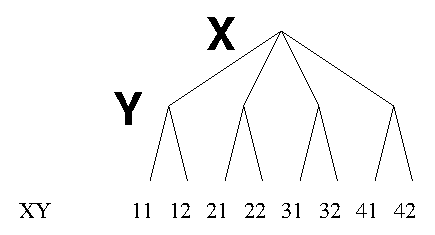
\epsfig{file=cimke1.eps,width=0.2\textwidth}}}
\br
{\tt | ?- }\parbox[t]{0.3\textwidth}{\tt
X in 1..4, 
Y in 1..2,\\
indomain(Y),\\
indomain(X).
}\raisebox{-1.5ex}{\parbox[c]{0.2\textwidth}{%\vspace*{-1ex} 
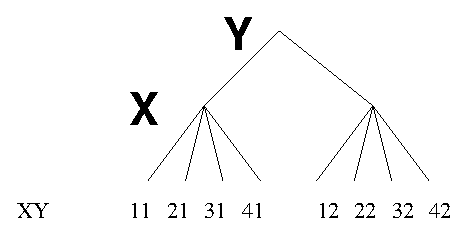
\epsfig{file=cimke2.eps,width=0.2\textwidth}}}
\br
Ha feltételezzük, hogy a fenti keresés során egyes ágak meghiúsulhatnak, akkor könnyen
rájöhetünk, hogy érdemesebb a második ábra szerinti keresési teret választani, mert ha
itt a kezdõ csomópontból kimenõ egyik ág meghiúsul, akkor azzal már helybõl 4 eset
ellenõrzését spóroltuk meg. Ez az úgynevezett \emph{first-fail} elv: elõbb címkézzük
a kisebb tartományú változót, ezzel remélhetõleg kevesebb választási pont lesz,
csökken a keresési tér mérete. Az is elõfordulhat, hogy egyes feladattípusokhoz saját,
speciális sorrend a célszerû: például az N királynõ feladatban célszerû elõbb a középsõ
sorokba elhelyezni a királynõket, mert ezek jobban megszûrik a maradék változók
értékkészletét, mint a szélsõ sorokba helyezett királynõk.
\br
A \clpfd könyvtár beépített címkézõ eljárása, a \cd{labeling/2} az elsõ paraméterként
átadott címkézési opció-listán keresztül lehetõséget ad arra, hogy a keresési tér
szerkezetét befolyásoljuk. Három lehetõség közül választhatunk:

\begin{itemize}
\item \emph{Felsorolás (\cd{enum})} --- többszörös választási pontot hoz létre, pontosan
annyi ággal, ahány lehetséges értéke van a változónak. Egy ágon mindig ezen értékek
közül pontosan az egyikre történik behelyettesítés. Használatára példa: \\
\cd{| ?- X in 1..4, labeling([enum],[X]).}
\item \emph{Kettévágás (\cd{bisect})} --- a változó tartományát megfelezi, és két ágat hoz
létre, értelemszerûen a két résztartományra való behelyettesítésével. Használatára példa: \\
\cd{| ?- X in 1..4, labeling([bisect],[X]).}
\item \emph{Lépegetés (\cd{step})} --- kiválaszt a változó tartományából egy értéket,
és két ágat hoz létre. Az egyik ágon erre az értékre szûkíti a változó tartományát,
a másik ágon pedig ezt az értéket kizárja a változó tartományából. Használatára példa: \\
\cd{| ?- X in 1..4, labeling([step],[X]).}
\end{itemize}

Az alábbi ábrákon egy 1..4 értékkészlettel rendelkezõ változó különbözõ címkézéseibõl
adódó keresési terek láthatóak.

\label{kerfak}
\begin{center}\begin{tabular}{ccc}

\epsfig{file=vpont_enum.eps,width=0.095\textwidth} &
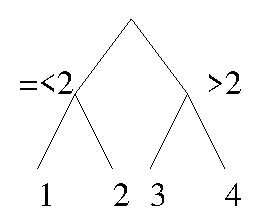
\epsfig{file=vpont_bisect.eps,width=0.1\textwidth} &
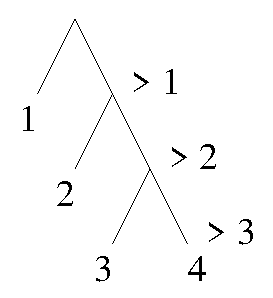
\epsfig{file=vpont_step.eps,width=0.1\textwidth} \\
Felsorolás (\cd{enum}) & Kettévágás (\cd{bisect}) & Lépegetés (\cd{step})
\end{tabular}\end{center}

Ezen ,,rövid'' bevezetõ után lássuk a \cd{labeling/2} címkézõ eljárás részletes
ismertetését!

\enumhead{A címkézés alap-eljárása:
\cd{labeling(Opciók, VáltozóLista)}}

A \cd{VáltozóLista} minden elemét minden lehetséges módon behelyettesíti,
az \cd{Opciók} lista által elõírt módon.  Az alábbi csoportok mindegyikébõl
legfeljebb egy opció szerepelhet. Hibát jelez, ha a \cd{VáltozóLista}-ban van
nem korlátos tartományú változó. Ha az elsõ négy csoport valamelyikébõl nem
szerepel opció, akkor a {\tt\em dõlt betûvel} szedett alapértelmezés lép életbe.

\begin{enumerate}
\item a változó kiválasztása: \cd{{\em leftmost}, min, max, ff, ffc,
variable(Sel)}. Ezek jelentése:
	\begin{itemize}
	\item \cd{leftmost} --- a változólista legbaloldalibb eleme.
	\item \cd{min} --- a legkisebb alsó határú. Ha több van, akkor ezek közül
	a legbaloldalibb.
	\item \cd{max} --- a legnagyobb felsõ határú. Ha több van, akkor ezek közül
	a legbaloldalibb.
	\item \cd{ff} --- \emph{first-fail} elv szerint a legkisebb tartományú
	(ld. \cd{fd_size/2} az \ref{fdset}. fejezetben). Ha több van, akkor ezek közül
	a legbaloldalibb.
	\item \cd{ffc} --- a legkisebb tartományú. Ha több ilyen van, akkor ezek
    	közül az, amelyikhez a legtöbb korlát kapcsolódik (\emph{most constrained} elv).
	Ha még mindig több ilyen van, akkor ezek közül a legbaloldalibb. Egy változóhoz
	kapcsolódó korlátok számát az \cd{fd_degree/2} adja meg (ld. \ref{fdset}. fejezet).
	\item \cd{variable(Sel)} --- testreszabott változó-kiválasztás: a következõ
	változó kiválasztása a \cd{Sel} felhasználói eljárás szerint történik. Bõvebben
	errõl a \pageref{variable:sel}. oldalon még lesz szó.
	\end{itemize}
\item a választási pont fajtája: \cd{{\em step}, enum, bisect, value(Enum)}. Ezek
jelentése:
	\begin{itemize}
	\item \cd{step} --- \cd{X \#= B} és \cd{X \#\bs= B} közti választás, ahol
	\cd{B} az \cd{X} tartományának alsó vagy felsõ határa, a bejárási iránytól
	függõen
	\item \cd{enum} --- többszörös választás \cd{X} lehetséges értékei közül
	\item \cd{bisect} --- \cd{X \#< M} és \cd{X \#>= M} közti választás, ahol
	\cd{M} az \cd{X} tartományának középsõ eleme.
	\item \cd{value(Enum)} --- testreszabott választás: \cd{Enum} egy felhasználói
	eljárás, amelynek szerepe, hogy leszûkítse X tartományát. Bõvebben errõl
	az \pageref{value:enum}. oldalon még lesz szó.
	\end{itemize}
\item a bejárási irány: \cd{{\em up}, down}. \cd{up} értelemszerûen alulról felfelé,
\cd{down} felülrõl lefelé járja be a tartományt. Csak \cd{step} típusú
címkézésnél van szerepe.
\item a keresett megoldások: \cd{{\em all}, minimize(X), maximize(X)}. Ezek jelentése:
	\begin{itemize}
	\item \cd{all} -- az összes megoldást megkeresi
	\item \cd{minimize(X)} -- azt a megoldást adja vissza, melyben \cd{X} értéke
	minimális.
	\item \cd{maximize(X)} -- azt a megoldást adja vissza, melyben \cd{X} értéke
	maximális.
	\end{itemize}
\item a gyûjtendõ statisztikai adat: \cd{assumptions(A)}. A keresés végén egyesíti
\cd{A} értékét a sikeres megoldáshoz vezetõ ágon lévõ változó-kiválasztások
számával (ami lényegében a keresési út hosszát jelenti).
\item a balszélsõ ágtól való eltérés korlátozása: \cd{discrepancy(D)}. Ezzel azt
korlátozzuk, hogy a keresés során maximum \cd{D}-szer választhatunk a választási
pontokban nem legbaloldalibb ágat. Akkor hasznos, ha a probléma megoldására van
valamiféle heurisztikánk, és úgy alakítjuk ki a keresési teret, hogy a heurisztika
szerinti optimális választást a legbaloldalibb ág tartalmazza. Mivel a heurisztika
nem teljesen tökéletes, ezért valamekkora eltérést megengedünk (ezt szabályozzuk
\cd{D} értékével). Ezt a módszert hívjuk \emph{Limited Discrepancy Search}-nek (LDS).
\end{enumerate}

A fenti pontokra való hivatkozással a \cd{labeling/2} eljárás pontos mûködése
így fest:

\label{labeling:lepesek}
\begin{description}
\item[a.]  Ha a változólista üres, akkor a címkézés sikeresen véget
ér. Egyébként kiválasztunk belõle egy \cd{X} elemet az 1. csoportbeli opció
által elõírt módon.
\item[b.] Ha \cd{X} behelyettesített, akkor a változólistából elhagyjuk, és az
{\bf a.} pontra megyünk.
\item[c.] Egyébként az \cd{X} változó tartományát felosztjuk két vagy több
diszjunkt részre a 2. csoportbeli opció szerint (kivéve \cd{value(Enum)}
esetén, amikor is azonnal az {\bf e.} pontra megyünk).
\item[d.] A tartományokat elrendezzük a 3. csoportbeli opció szerint.
\item[e.] Létrehozunk egy választási pontot, amelynek ágain sorra
leszûkítjük az \cd{X} változót a kiválasztott tartományokra.
\item[f.] Minden egyes ágon az \cd{X} szûkítése értelemszerûen kiváltja a
rá vonatkozó korlátok felébredését. Ha ez meghiúsulást okoz, akkor
visszalépünk az {\bf e.} pontra és ott a következõ ágon folytatjuk.
\item[g.] Ha \cd{X} most már behelyettesített, akkor elhagyjuk a változólistából.
Ezután mindenképpen folytatjuk az {\bf a.} pontnál.
\item[h.] Eközben értelemszerûen követjük a 4-6. csoportbeli opciók elõírásait is.
\end{description}

Lássunk egy példát az \fdbg nyomkövetõ könyvtár (\ref{fdbg}. fejezet) használatával!
\br
\begin{verbatim}
| ?- fdbg_assign_name(X, x), fdbg_assign_name(Y, y), 
     X in 1..3, Y in 1..2, X #>= Y, fdbg_on, 
     labeling([min], [X,Y]).
% The clp(fd) debugger is switched on
Labeling [1, <x>]: starting in range 1..3.
Labeling [1, <x>]: step: <x> = 1
    <y>#=<1     y = 1..2 -> {1} Constraint exited.
                                                X = 1, Y = 1 ? ;
Labeling [1, <x>]: step: <x> >= 2
    <y>#=<<x>   y = 1..2, x = 2..3  Constraint exited.
    Labeling [6, <y>]: starting in range 1..2.
    Labeling [6, <y>]: step: <y> = 1
        Labeling [8, <x>]: starting in range 2..3.
        Labeling [8, <x>]: step: <x> = 2
                                                X = 2, Y = 1 ? ;
        Labeling [8, <x>]: step: <x> >= 3
                                                X = 3, Y = 1 ? ;
        Labeling [8, <x>]: failed.
    Labeling [6, <y>]: step: <y> >= 2
        Labeling [12, <x>]: starting in range 2..3.
        Labeling [12, <x>]: step: <x> = 2
                                                X = 2, Y = 2 ? ;
        Labeling [12, <x>]: step: <x> >= 3
                                                X = 3, Y = 2 ? ;
        Labeling [12, <x>]: failed.
    Labeling [6, <y>]: failed.
Labeling [1, <x>]: failed.
\end{verbatim}

A keresési fa:

\begin{center}
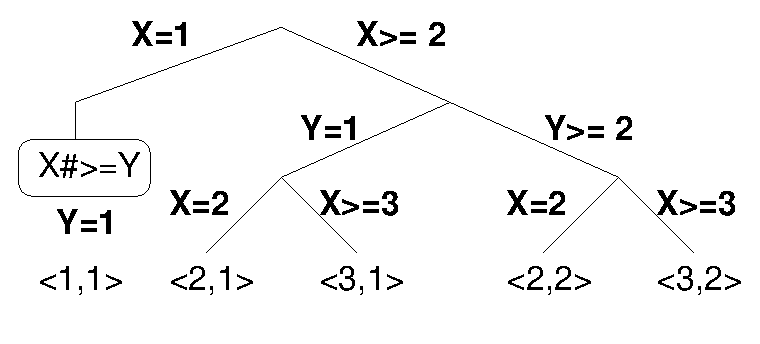
\epsfig{file=cimke_pelda.eps,width=0.4\textwidth}
\end{center}

Egy másik példa, ezúttal szélsõérték-számításra:

\begin{verbatim}
| ?- _L=[X,Y,Z], domain(_L, 0, 1), V#=Y+Z-X, labeling([minimize(V)], _L).
V = -1, X = 1, Y = 0, Z = 0 ? ;
no
\end{verbatim}

A keresési fa (branch-and-bound algoritmussal):

\begin{center}
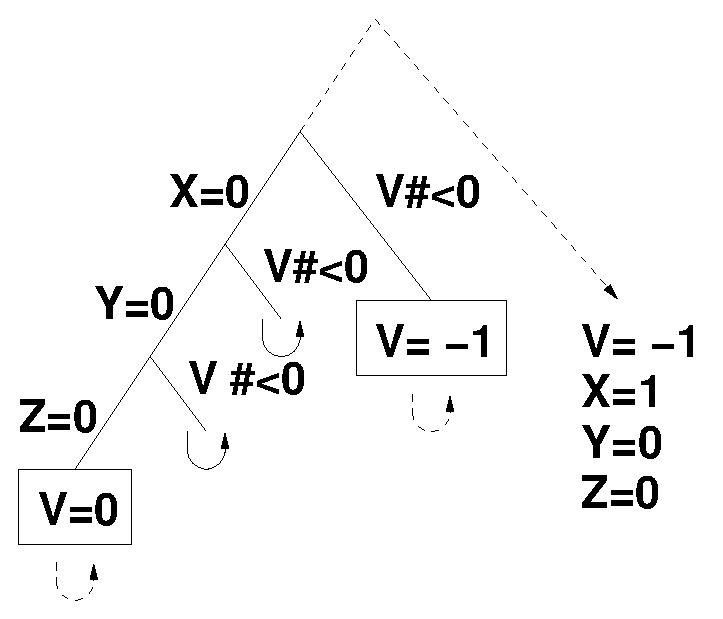
\epsfig{file=bb-pelda.eps,width=0.4\textwidth}
\end{center}

A branch-and-bound algoritmus itt elõször megkeresi az elsõ megoldást, majd innentõl
kezdve a további ágak végigjárása során korlátként felveszi azt is, hogy a megoldásnak
kisebbnek kell lennie, mint az eddig megtalált legkisebb. Ha ezzel a feltétellel is
talál újabb megoldást, akkor innentõl kezdve a többi ágon már ezzel az újabb minimummal
dolgozik, egészen addig, amíg be nem járja a teljes keresési teret.
\br
A statisztikai funkciót  és a bal szélsõ ágtól való eltérés korlátozását bemutató példa
(érdemes összevetni az eredményeket a \pageref{kerfak}. oldalon látható keresési
fákkal):

\begin{alltt}
% a Select címkézési mód használatával megkeresi az X in 1..4 korlát összes
% megoldását, és a megoldásokhoz vezetõ utak hosszát As-ben adja vissza
assumptions(Select, As) :-
     X in 1..4, findall(A, labeling([Select, assumptions(A)], [X]), As).

% a Select címkézési mód és D eltérés-korlát használatával megkeresi az
% X in 1..4 korlát összes megoldását, és a megtalált megoldásokat visszaadja
% Xs-ben
lds(Select, D, Xs) :-
     X in 1..4, findall(X, labeling([Select, discrepancy(D)], [X]), Xs).

| ?- assumptions(enum, As).          As = [1,1,1,1] ? ; no
| ?- assumptions(bisect, As).        As = [2,2,2,2] ? ; no
| ?- assumptions(step, As).          As = [1,2,3,3] ? ; no 
                                                                          
| ?- lds(enum, 1, Xs).               Xs = [1,2,3,4] ? ; no 
| ?- lds(bisect, 1, Xs).             Xs = [1,2,3] ? ; no 
| ?- lds(step, 1, Xs).               Xs = [1,2] ? ; no 
\end{alltt}

Látható, hogy \cd{enum} címkézési módnál minden megoldáshoz 1 hosszú út vezet,
mivel egy többszörös választási pontot hoztunk létre. Éppen ezért az a korlátozásunk,
hogy a legbaloldalibb ágtól maximum egyszer térhetünk el, nem jelent semmi pluszt,
mind a négy megoldást meg tudjuk így keresni.
\br
\cd{bisect} címkézésnél minden megoldáshoz egy 2 hosszú út vezet, hiszen az
elsõ választási pontban az \cd{X \#< 3} és \cd{X \#>= 3} korlátok felvétele között
választunk, a második választási pontban pedig a megmaradó 2 méretû tartományokat
felezzük tovább. A legbaloldalibb ágtól való eltérésre vonatkozó korlátunk így nem
találja meg a 4-et, mint megoldást, mert ahhoz elõször az \cd{X \#>= 3} ágat, másodszor
pedig az \cd{X = 4} ágat kéne választanunk, és mindkettõ jobb oldali ág.
\br
\cd{step} címkézésnél az 1-hez, mint megoldáshoz 1 hosszú út vezet, mert az elsõ
választási pontban az \cd{X = 1} és \cd{X \#= 1} korlátok között döntünk. A 2-t így
már csak két lépésben tudjuk megtalálni, a 3-at és a 4-et pedig hasonló módon csak
3-3 lépésben. Mivel a bal oldali út itt mindig az \cd{X} valamely értékre való kötését
jelenti, és csak egyszer léphetünk jobb oldalra, ezért csak az 1-et és a 2-t fogjuk
megtalálni, hiszen a 3-hoz már kétszer, a 4-hez már háromszor kéne jobbra lépnünk.
\br
\label{variable:sel}
Mint azt már néhány oldallal elõbb említettük, a felhasználónak a \cd{labeling/2}
eljárás \cd{variable(Sel)} opcióján keresztül lehetõsége van egy saját változó-kiválasztó
eljárás írására is. Az eljárást \cd{Sel(Vars, Selected, Rest)} alakban hívja meg a rendszer,
ahol \cd{Vars} a még címkézendõ változók/számok listája. \cd{Sel} feladata, hogy
determinisztikusan egyesítse \cd{Selected}-et a következõ címkézendõ \emph{változóval},
\cd{Rest}-et pedig a maradékkal. \cd{Sel} egy tetszõleges meghívható kifejezés lehet,
a három argumentumot a rendszer fûzi \cd{Sel} argumentumainak végére, így a \cd{Sel}
által hivatkozott eljárás akár 3-nál több paraméterrel is rendelkezhet. A példa egy olyan
kiválasztást valósít meg, ahol a felhasználó szabályozhatja, hogy hányadik változót
válasszuk ki a változó-listából.

\begin{verbatim}
% A Vars-beli változók között Sel a Hol-adik, ha a lista teljes hosszát
% 1-nek vesszük (Hol így egy törtszám). Rest a maradék.
valaszt(Hol, Vars, Sel, Rest) :-
        szur(Vars, Szurtek), 
        length(Szurtek, Len), N is integer(Hol*Len),
        nth0(N, Szurtek, Sel, Rest).

% szur(Vk, Szk): A Vk-ban levõ változók listája Szk.
szur([], []).
szur([V|Vk], Szk) :- nonvar(V), !, szur(Vk, Szk).
szur([V|Vk], [V|Szk]) :- szur(Vk, Szk).
\end{verbatim}

\label{value:enum}
Lehetõség van a kiválasztott változó tartományának szûkülését is befolyásolni. Ehhez a
\cd{labeling/2} opció-listájában a \cd{value(Enum)} opciót kell megadnunk. \cd{Enum}-ot
a rendszer \cd{Enum(X, Rest, BB0, BB)} alakban hívja meg, ahol \cd{[X|Rest]} a címkézendõ
változók listája, és ebbõl \cd{X}-et kell az eljárásnak címkéznie, mégpedig
nemdeterminisztikus módon \cd{X} tartományát az összes kívánt módon szûkítve (tehát
a \cd{value(Enum)} a \pageref{labeling:lepesek}. oldalon lévõ lépések közül a
{\bf c.}, {\bf d.} és {\bf e.} lépéseket váltja ki). \cd{BB} és \cd{BB0} értéke számunkra
csak annyiból lényeges, hogy az elsõ választásnál meg kell hívni \cd{first_bound(BB0, BB)}-t,
a másodiknál pedig \cd{later_bound(BB0, BB)}-t a branch-and-bound, illetve LDS módszerek
kiszolgálására. \cd{Enum} egy meghívható kifejezés, a 4 paramétert a rendszer fûzi \cd{Enum}
argumentumlistájának végére. Példaként tekintsünk egy olyan címkézõ eljárást, amely
az értékeket az értéklistában belülrõl kifelé haladva sorolja fel:

\begin{verbatim}
midout(X, _Rest, BB0, BB) :-
        fd_size(X, Size),
        Mid is (Size+1)//2,
        fd_set(X, Set), 
        fdset_to_list(Set, L),
        nth(Mid, L, MidElem),
        (   first_bound(BB0, BB), X = MidElem
        ;   later_bound(BB0, BB), X #\= MidElem
        ).

| ?- X in {1,3,12,19,120}, 
     labeling([value(midout)], [X]).
X = 12 ? ;
X = 3 ? ;
X = 19 ? ;
X = 1 ? ;
X = 120 ? ; no
\end{verbatim}

Végül, a címkézés testreszabásának fontosságát bizonyítandó, nézzük meg az N királynõ
feladat megoldását különféle címkézõ módszerekkel (600 MHz-es Pentium III gépen):

\begin{center}
\enumhead{Összes megoldás keresése}
\begin{tabular}{|l|rr|rr|rr|}
\hline
méret           & \multicolumn{2}{c|}{ n=8}    & \multicolumn{2}{c|}{ n=10}    & \multicolumn{2}{c|}{ n=12}    \\
\hline
megoldások száma       & \multicolumn{2}{c|}{92}    & \multicolumn{2}{c|}{
724}    & \multicolumn{2}{c|}{ 14200}    \\
\hline
címkézés                     & sec & btrk & sec & btrk & sec & btrk \\
\hline
\hline
\cd{[step]}                 & 0.07 & 324 & 1.06 & 5942 & 25.39 & 131K \\ \hline
\cd{[enum]}                 & 0.07 & 324 & 1.03 & 5942 & 24.84 & 131K \\ \hline
\cd{[bisect]}               & 0.07 & 324 & 1.07 & 5942 & 26.04 & 131K \\ \hline \hline
\cd{[enum,min]}             & 0.08 & 462 & 1.31 & 8397 & 33.89 & 202K \\ \hline
\cd{[enum,max]}             & 0.07 & 462 & 1.31 & 8397 & 33.89 & 202K \\ \hline
\cd{[enum,ff]}              & 0.06 & 292 & 0.97 & 4992 & 21.57 & 101K \\ \hline
\cd{[enum,ffc]}             & 0.06 & 292 & 1.04 & 4992 & 23.24 & 101K \\ \hline
\cd{[enum,{\em midvar}\footnotemark[1]]\footnotemark[2]}    & 0.06 & 286 & 0.90 & 4560 & 20.11 &  88K \\ \hline
\end{tabular}
\end{center}

\begin{center}
\enumhead{Elsõ megoldás keresése}
\begin{tabular}{|l|rr|rr|rr|}
\hline
méret           & \multicolumn{2}{c|}{ n=16}    & \multicolumn{2}{c|}{ n=18}    & \multicolumn{2}{c|}{ n=20}    \\
\hline
címkézés                     & sec & btrk & sec & btrk & sec & btrk \\
\hline
\hline
\cd{[enum]}                 & 0.43 & 1833 & 1.76 &  7436 &  9.01 & 37320\\ \hline
\cd{[enum,min]}             & 0.52 & 2095 & 0.87 &  2595 &  1.39 &  3559\\ \hline
\cd{[enum,max]}             & 0.61 & 3182 & 2.68 & 13917 & 16.06 & 83374\\ \hline
\cd{[enum,ff]}              & 0.03 &    7 & 0.05 &    11 &  0.08 &    33\\ \hline
\cd{[enum,ffc]}             & 0.03 &    7 & 0.05 &    11 &  0.09 &    33\\ \hline
\cd{[enum,{\em midvar\footnotemark[1]}]\footnotemark[2]}    & 0.04 &   69 & 0.06 &    57 &  0.15 &   461\\ \hline
\cd{[value(midout)\footnotemark[2]]}        & 0.04 &    3 & 0.05 &     4 &  0.09 &    38\\ \hline
\cd{[value(midout)\footnotemark[2],ffc]}    & 0.04 &   15 & 0.06 &    41 &  0.08 &    20\\ \hline
\end{tabular}
\end{center}

\footnotetext[1]{{\tt{\em midvar} $\equiv$ variable(valaszt(0.5))}.}
\footnotetext[2]{Hatékonyabb statikusan (a címkézés elõtt egyszer) elrendezni a változókat
és az értékeket, \\ lásd az {\tt alt_queens/2} eljárást a \cd{library('clpfd/examples/queens')} állományban.}

%% bele kéne venni a 91. oldalon lévõ részt is???? (szélsõértékek ismételt hívással való
%% elõállítása témakör)

\subsection{Kombinatorikus korlátok}

Az ebben a fejezetben ismertetett globális korlátok az eddigiekhez hasonlóan
nem tükrözhetõek. Minden olyan helyen, ahol a korlátok FD-változót várnak,
írhatunk számértéket is.

\subsubsection{Értékek számolása és különbözõsége}

\medskip

{\bcd{count(Val, List, {\em Relop}, Count)}}

Jelentése: a \cd{Val} egész szám a \cd{List} FD-változó-listában $n$-szer fordul elõ,
és fennáll az  {\it n} \cd{{\em Relop} Count} reláció. Itt \cd{Count} FD változó,
\cd{\em Relop} pedig a hat összehasonlító reláció egyike: \cd{\#=, \#\bs=, \#<} \ldots.
Tartomány-szûkítést biztosít.

\medskip

{\bcd{global_cardinality(Vars, Vals)}}

\cd{Vars} egy FD változókból álló lista, \cd{Vals} pedig  \cd{I-K} alakú párokból
álló lista, ahol \cd{I} egy egész, \cd{K} pedig egy FD változó. Mindegyik \cd{I}
érték csak egyszer fordulhat elõ a \cd{Vals} listában. Jelentése: A \cd{Vars}-beli
FD változók csak a megadott \cd{I} értékeket vehetik fel, és minden egyes \cd{I-K}
párra igaz, hogy a \cd{Vars} listában pontosan \cd{K} darab \cd{I} értékû elem van.
Ha \cd{Vals} vagy \cd{Vars} tömör, és még sok más speciális esetben tartomány-szûkítést
ad.

\medskip

\label{all_distinct}
{\bcd{all\_different(Vs{\em [}, Options{\em ]})\\
      all\_distinct(Vs{\em [}, Options{\em ]})}}

Jelentése: a \cd{Vs} FD változó-lista elemei páronként különbözõek.  
A korlát szûkítési mechanizmusát az \cd{Options} opció-lista szabályozza,
eleme lehet:

\begin{itemize}
\item \cd{consistency(Cons)} --- a szûkítési algoritmust szabályozza. \cd{Cons} lehet:
\begin{description}
\item[\cd{global}] --- tartomány-szûkítõ algoritmus (Regin), durván a
tartományok méretével arányos idejû (alapértelmezés \cd{all\_distinct} esetén)
\item[\cd{bound}] --- intervallum-szûkítõ algoritmus (Mehlhorn), a
változók és értékek számával arányos idejû
\item[\cd{local}] --- a nemegyenlõség páronkénti felvételével azonos
szûkítõ erejû algoritmus, durván a változók számával arányos idejû
(alapértelmezés \cd{all\_different} esetén).
\end{description}

\item \cd{on(On)} --- az ébredést szabályozza. \cd{On} lehet:
\begin{description}
\item[\cd{dom}] --- a változó tartományának bármiféle változásakor
ébreszt (alapértelmezés \cd{all\_distinct} esetén),
\item[{\rm \bf \cd{min}, \cd{max}, {\rm ill.} \cd{minmax}}] ---
a változó tartományának adott ill. bármely határán történõ változáskor ébreszt,
\item[\cd{val}] --- a változó behelyettesítésekor ébreszt csak (alapértelmezés
\cd{all\_different} esetén).
\end{description}

A \cd{consistency(local)} beállításnál nincs értelme \cd{val}-nál
korábban ébreszteni, mert ez a szûkítést nem befolyásolja.
\end{itemize}

A különbözõ ébresztési és szûkítési módok bemutatásához nézzük az alábbi predikátumot:

\begin{verbatim}
pelda(Z, I, On, C) :-
     L = [X,Y,Z], domain(L, 1, 3), 
     all_different(L, [on(On),consistency(C)]), X #\= I, Y #\= I.
\end{verbatim}

\begin{tabular}{ll}
\verb'| ?- pelda(Z, 3, dom, local).'    & $\rightarrow$ \verb'  Z in 1..3 '  \\
\verb'| ?- pelda(Z, 3, min, global).'   & $\rightarrow$ \verb'  Z in 1..3 '  \\
\verb'| ?- pelda(Z, 3, max, bound).'    & $\rightarrow$ \verb'  Z = 3     '  \\
\verb'| ?- pelda(Z, 2, minmax, global).'& $\rightarrow$ \verb'  Z in 1..3 '  \\
\verb'| ?- pelda(Z, 2, dom, bound).'    & $\rightarrow$ \verb'  Z in 1..3 '  \\
\verb'| ?- pelda(Z, 2, dom, global).'   & $\rightarrow$ \verb'  Z = 2     '  \\
\end{tabular}
\br
Látható, hogy csak a harmadik és a hatodik példa jön rá arra, hogy \cd{Z} csak
a második paraméterben megadott érték lehet. Az elsõ és az ötödik példa a \cd{local},
illetve \cd{bound} algoritmus gyengesége miatt nem végzi el a szûkítést, a második
és a negyedik pedig a nem megfelelõ ébresztési feltétel miatt.

\subsubsection{Függvénykapcsolatok és relációk}

{\bcd{element(X, List, Y)}}

Jelentése: \cd{List} \cd{X}-edik eleme \cd{Y} (1-tõl számozva). Itt \cd{X} és \cd{Y}
FD változók, \cd{List} FD változókból álló lista. Az \cd{X} változóra nézve
tartomány-szûkítést, az \cd{Y} és \cd{List} változókra nézve intervallum-szûkítést
biztosít. 

Példák: 

\begin{verbatim}
| ?- element(X, [0,1,2,3,4], Y), X in {2,5}.  % ekvivalens Y #= X-1-gyel
X in {2}\/{5}, Y in 1..4 ?                    % intervallum-konzisztens
| ?- element(X, [0,1,2,3,4], Y), Y in {1,4}.
X in {2}\/{5}, Y in {1}\/{4} ?                % tartomány-konzisztens

% X #= C #<=> B megvalósítása, 1=<{X,C}=<6 esetére
% (C konstans).
beq(X, C, B) :- 
        X in 1..6, call(I #= X+6-C), 
        element(I, [0,0,0,0,0,1,0,0,0,0,0], B).
\end{verbatim}

\medskip
{\bcd{relation(X, Rel, Y)}}

Itt \cd{X} és \cd{Y} FD változók, \cd{Rel} formája: egy lista
{\tt\em Egész-KonstansTartomány} alakú párokból (ahol mindegyik {\tt\em Egész}
csak egyszer fordulhat elõ). Jelentése: \cd{Rel} tartalmaz egy \cd{X-Tart} párt,
ahol \cd{Y} eleme a \cd{Tart}-nak, azaz: \[ \cd{relation(X,H,Y)} \equiv \tuple{\cd{X,Y}}
\in \{\tuple{x,y}|x-\cd{T} \in \cd{H}, y \in \cd{T}\}\] Tetszõleges bináris reláció
definiálására használható, tartomány-szûkítést biztosít. Példa:

\begin{verbatim}
'abs(x-y)>1'(X,Y) :-
        relation(X, [0-(2..5), 1-(3..5), 2-{0,4,5},
                     3-{0,1,5}, 4-(0..2), 5-(0..3)], Y).

| ?- 'abs(x-y)>1'(X,Y), X in 2..3.
Y in (0..1) \/ (4..5) ? ;
no
\end{verbatim}

\medskip
{\bcd{case(Template, Tuples, DAG{\em [}, Options{\em ]})}}

Jelentése: A \cd{Tuples} lista minden elemét illesztve a \cd{Template}
mintára, a \cd{DAG} által leírt reláció fennáll. Az ébresztést és a
szûkítést az \cd{Options} opció-lista szabályozza (hasonló módon, mint
az \cd{all_distinct} esetén, lásd \pageref{all_distinct}. oldal és 
SICStus kézikönyv). Alaphelyzetben minden változásra ébred és
tartomány-szûkítést ad.

A \cd{DAG} csomópontok listája, az elsõ elem a kezdõpont. Egy csomópont
alakja: \cd{node(ID, X, Successors)}. Itt \cd{ID} a csomópont azonosítója
(egész vagy atom), \cd{X} a vizsgálandó változó. Belsõ gráfpont esetén
\cd{Successors} a rákövetkezõ csomópontok listája, elemei \cd{Min..Max)-ID2}
alakúak. Egy ilyen elem jelentése: ha \cd{Min} $\leq$ \cd{X} $\leq$ \cd{Max},
akkor menjünk az \cd{ID2} csomópontra. Végpont esetén \cd{Successors} a
végfeltételek listája, elemei \cd{Min..Max} alakúak, jelentése pedig: ha
valamelyik elem esetén \cd{Min} $\leq$ \cd{X} $\leq$ \cd{Max} fennáll, akkor
a reláció teljesül.
\br
Példaként tekintsük az alábbi gráfot, amely az ,,\cd{X}, \cd{Y} és \cd{Z}
felének egészrésze mind más'' (\([\frac{\cd{X}}{\cd{2}}]\neq[\frac{\cd{Y}}{\cd{2}}],
[\frac{\cd{X}}{\cd{2}}]\neq[\frac{\cd{Z}}{\cd{2}}],
[\frac{\cd{Y}}{\cd{2}}]\neq[\frac{\cd{Z}}{\cd{2}}]\)) relációt írja le a 0..5
tartományon:

\begin{center}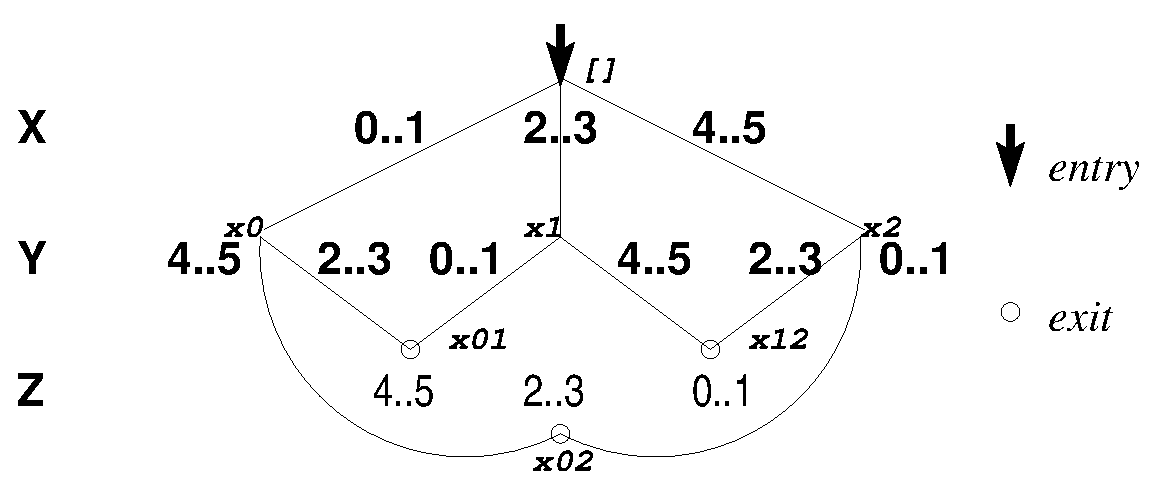
\epsfig{file=case.eps,width=0.7\textwidth}\end{center}

Ennek megvalósítása a \cd{case/3} korláttal:

\begin{verbatim}
felemasok(X, Y, Z) :-
   case(f(A,B,C), [f(X,Y,Z)],
        [node([], A, [(0..1)-x0,(2..3)-x1,(4..5)-x2]),
         node(x0, B, [(2..3)-x01,(4..5)-x02]),
         node(x1, B, [(0..1)-x01,(4..5)-x12]),
         node(x2, B, [(0..1)-x02,(2..3)-x12]),
         node(x01,C,[4..5]), node(x02,C,[2..3]), node(x12,C,[0..1])
        ]).
\end{verbatim}

Példa többszörös mintára: \cd{case(T,[A$_1$,$\ldots$],D)$\equiv$case(T,[A$_1$],D),$\ldots$}

\begin{verbatim}
felemasok_vacak(X, Y, Z) :-
    case(A\=B, [X\=Y,X\=Z,Y\=Z],
     [node(root, A, [(0..1)-0,(2..3)-1,(4..5)-2]),
      node(0,B,[2..5]),node(1,B,[0..1,4..5]),node(2, B, [0..3])
     ], [on(val(X)),on(val(Y)),on(val(Y))/*,prune(val(X)), ...*/]).
\end{verbatim}

\subsubsection{Leképezések, gráfok}

{\bcd{sorting(X, I, Y)}}

Az \cd{X} FD-változókból álló lista rendezettje az \cd{Y} FD-változó-lista. Az \cd{I}
FD-változó-lista írja le a rendezéshez szükséges permutációt. Azaz: mindhárom
paraméter azonos ($n$) hosszúságú, \cd{Y} rendezett, \cd{I} az \cd{1..$n$} számok
egy permutációja, és $\forall i \in$ \cd{1..$n$} esetén \cd{X$_i$ =Y$_{\cd{I}_i}$}. 

\medskip

{\bcd{assignment(X, Y{\em [}, Options{\em ]})}}

\cd{X} és \cd{Y} FD változókból alkotott azonos ($n$) hosszúságú listák. Teljesül,
ha \cd{X$_i$} és \cd{Y$_i$} mind az \cd{1..$n$} tartományban vannak és \cd{X$_i$=$j$} 
$\Leftrightarrow$ \cd{Y$_j$=$i$}. Másképpen fogalmazva: \cd{X} egy-egyértelmû
leképezés az \cd{1..$n$} halmazon (az \cd{1..$n$} számok egy permutációja), és
\cd{Y} az \cd{X} inverze.

Az \cd{Options} lista ugyanolyan, mint az \cd{all\_different/[1,2]} korlát
esetében (ld. \pageref{all_distinct}. oldal), az alapértelmezés
\cd{[on(domain),consistency(global)]}.

\medskip

{\bcd{circuit(X)} }

\cd{X} $n$ hosszúságú lista. Igaz, ha minden \cd{X$_i$} az \cd{1..$n$}
tartományba esik, és \cd{X$_1$, X$_{\cd{X}_1}$, X$_{\cd{X}_{\cd{X}_1}}$... }
($n$-szer ismételve) az \cd{1..$n$} számok egy permutációja. Másképp: \cd{X} egy
egyetlen ciklusból álló permutációja az \cd{1..$n$} számoknak.

Gráfokon vett értelmezés: legyen egy $n$ szögpontú irányított gráfunk,
jelöljük a pontokat az \cd{1..$n$} számokkal. Vegyünk fel $n$ db FD-változót,
\cd{X$_i$} tartománya álljon azon $j$ számokból, amelyekre $i$-bõl vezet $j$-be él.
Ekkor \cd{circuit(X)} azt jelenti, hogy az $i$ $\rightarrow$ \cd{X$_i$} élek a
gráf egy Hamilton-körét adják.

\medskip

{\bcd{circuit(X, Y)}}

Ekvivalens a következõvel: \cd{circuit(X), assignment(X, Y)}. Gráfokon értelmezve
megadja a Hamilton-kört és annak az ellenkezõ irányban vett bejárását is.

Példák az \cd{assignment/2} és a \cd{circuit/2} használatára:

\begin{verbatim}
| ?- length(L, 3), domain(L, 1, 3), assignment(L, LInv), L=[2|_], 
     labeling([], L).
L = [2,1,3], LInv = [2,1,3] ? ;
L = [2,3,1], LInv = [3,1,2] ? ;
no
| ?- length(L, 3), domain(L, 1, 3), circuit(L, LInv), L=[2|_].
L = [2,3,1], LInv = [3,1,2] ? ;
no
\end{verbatim}

Kicsit ,,életszagúbb'' példa:

\medskip

\begin{tabular}{cp{0.8\textwidth}}
\begin{tabular}{|c|c|c|}
\hline 1 & 2 & 2 \\ \hline 3 & 1 & 3 \\ \hline 4 & 4 & 1 \\ \hline
\end{tabular} &
\vspace{-1.5\baselineskip}
Adott a bal oldalt látható 3 $\times$ 3-as négyzetrács. Feladat: járjuk be
a rács elemeit a bal felsõ sarokból indulva úgy, hogy minden cellán pontosan
egyszer haladunk át, és $n$-t tartalmazó celláról csak $n+1$-et tartalmazóra
léphetünk (kivéve $n=4$ esetben, innen csak 1-est tartalmazóra). \\
\end{tabular}

\begin{verbatim}
| ?- L=[_1,_2,_3,_4,_5,_6,_7,_8,1], _1=2, _2 in {4,6}, _3=6, 
     _4 in {7,8}, _5 in {2,3}, _6=8, _7=5, _8 in {5,9}, 
     circuit(L).
L = [2,4,6,7,3,8,5,9,1] ? ; no
\end{verbatim}

Az eredmény-listában minden elem megadja, hogy az elemnek megfelelõ cella után
melyik cella következik a körben (a cellákat fentrõl lefelé és balról jobbra
számoztuk be 1-tõl 9-ig).
\br
A \cd{circuit/1} felhasználható az utazó ügynök probléma megoldására is:

\begin{verbatim}
:- module(tsp, [tsp/3]).
:- use_module(library(clpfd)).
:- use_module(library(lists), [append/3]).

tsp(Lab, Successor, Cost) :-
        Successor = [X1,X2,X3,X4,X5,X6,X7],
        Costs = [C1,C2,C3,C4,C5,C6,C7],
        element(X1, [0,205,677,581,461,878,345], C1),
        element(X2, [205,0,882,427,390,1105,540], C2),
        element(X3, [677,882,0,619,316,201,470], C3),
        element(X4, [581,427,619,0,412,592,570], C4),
        element(X5, [461,390,316,412,0,517,190], C5),
        element(X6, [878,1105,201,592,517,0,691], C6),
        element(X7, [345,540,470,570,190,691,0], C7),
        sum(Costs, #=, Cost),
        Predecessor = [Y1,Y2,Y3,Y4,Y5,Y6,Y7],
        Costs2 = [D1,D2,D3,D4,D5,D6,D7],
        element(Y1, [0,205,677,581,461,878,345], D1),
        element(Y2, [205,0,882,427,390,1105,540], D2),
        element(Y3, [677,882,0,619,316,201,470], D3),
        element(Y4, [581,427,619,0,412,592,570], D4),
        element(Y5, [461,390,316,412,0,517,190], D5),
        element(Y6, [878,1105,201,592,517,0,691], D6),
        element(Y7, [345,540,470,570,190,691,0], D7),
        sum(Costs2, #=, Cost),
        circuit(Successor, Predecessor),
        append(Successor, Predecessor, All),
        labeling([minimize(Cost)|Lab], All).

| ?- tsp([ff], Succs, Cost).
Cost = 2276, Succs = [2,4,5,6,7,3,1] ? 
\end{verbatim}

\subsubsection{Ütemezési korlátok}

{\bcd{cumulative(Starts, Durations, Resources, Limit{\em[}, Opts{\em ]})}}

Jelentése: a \cd{Starts} kezdõidõpontokban elkezdett, \cd{Durations} ideig tartó
és \cd{Resources} erõforrásigényû feladatok bármely idõpontban összesített
erõforrásigénye nem haladja meg a \cd{Limit} határt (és fennállnak az opcionális
precedencia korlátok). Az elsõ három argumentum FD változókból álló, egyforma ($n$)
hosszú lista, a negyedik egy FD változó. 

\medskip

{\bcd{serialized(Starts, Durations{\em [}, Opts{\em ]})}}

A \cd{cumulative} speciális esete, ahol az összes erõforrás-igény és a korlát is 1.

\br
Vezessük be a \cd{cumulative($S,D,R,Lim$ \dots )} híváshoz az alábbi jelöléseket:

\begin{quote}
$a = min(S_1,\ldots,S_n)$ {\rm $a$ a kezdõidõpont)} \\
$b = max(S_1+D_1,\ldots,S_n+D_n)$ {\rm $b$ a (végidõpont)}\\
$R_{ij} = R_j$, ha  $S_j \leq i < S_j+D_j$,
        egyébként $R_{ij} = 0$; {\rm $R_{ij}$ (a $j$. feladat erõforrásigénye
        az $i$. idõpontban)}
\end{quote}

Ezekkel a jelölésekkel a korlát jelentése (a precedencia-korlátok nélkül):

\begin{quote}
$R_{i1}+\ldots+R_{in} \leq Lim$ minden $a \leq i < b$ esetén.
\end{quote}

Az \cd{Opts} opciólista a következõ beállításokat tartalmazhatja:

\begin{itemize}
\item \cd{precedences(Ps)} ---
          \cd{Ps} egy lista, amely precedencia korlátokat ír le. Elemei a következõk
          lehetnek (\cd{I} és \cd{J} feladatok sorszámai, \cd{D} egy pozitív
          egész, \cd{Tart} egy  konstans-tartomány):  
\begin{itemize}
\item\cd{d(I,J,D)}, jelentése: $S_\cd{I}+\cd{D} \leq S_\cd{J}$ vagy $S_\cd{J} \leq S_\cd{I}$
(tehát az \cd{I}. és a \cd{J}. feladat közti átállás egy holtidõvel modellezhetõ, és
\cd{D} az \cd{I}. feladat hossza ($D_\cd{I}$) plusz az átállási idõ. Ha azt akarjuk
megadni, hogy egy feladatot elõbb el kell végezni, mint egy másikat, akkor átállási
idõnek \cd{sup}-ot kell megadni.
\item\cd{I-J in Tart}, jelentése: \cd{$S_\cd{I}-S_\cd{J}$ \#= D$_\cd{IJ}$,
D$_\cd{IJ}$ in Tart}. Akkor használatos, ha az \cd{I}. és \cd{J}. feladat között
eltelt idõnek alsó és felsõ korlátja is van.
\end{itemize}

\item \cd{resource(R)} --- speciális ütemezési címkézéshez szükséges opció. \cd{R}-et
          egyesíti egy kifejezéssel, amelyet késõbb átadhatunk az \cd{order\_resource/2}
          eljárásnak, hogy felsoroltassuk a feladatok lehetséges sorrendjeit. Az
          \cd{order_resource/2} eljárásról bõvebben a \pageref{order_resource}. oldalon
          lesz szó.

\item \cd{decomposition(Boolean)} ---
          Ha \cd{Boolean} \cd{true}, akkor minden ébredéskor megpróbálja
          kisebb darabokra bontani a korlátot (pl. ha van két
          át nem lapoló feladathalmazunk, akkor ezeket külön-külön
          kezelhetjük, ami az algoritmusok gyorsabb lefutását
          eredményezheti). Alapértelmezésben ki van kapcsolva.

\item \cd{path\_consistency(Boolean)} ---
          Ha \cd{Boolean} \cd{true}, akkor figyeli a feladatok kezdési
          idõpontja közti különbségek konzisztenciáját. Ez egy olyan redundáns
          korlátra hasonlít, amely minden $i,j$ párra felveszi a
          \cd{SD$_{ij}$ \#= S$_j$ - S$_i$}, és minden $i,j,k$ hármasra a
          \cd{SD$_{ik}$ \#= SD$_{ij}$ + SD$_{jk}$} korlátot. Alapértelmezésben
          ki van kapcsolva.

\item \cd{static\_sets(Boolean)}
          Ha \cd{Boolean} \cd{true}, akkor, ha bizonyos feladatok sorrendje
          ismert, akkor ennek megfelelõen megszorítja azok kezdõ
          idõpontjait. Alapértelmezésben ki van kapcsolva. Például:
\begin{verbatim}
| ?- _S = [S1,S2,S3],  domain(_S, 0, 9), (SS = false ; SS = true),
     serialized(_S, [5,2,7], [static_sets(SS),
                              precedences([d(3,1,sup), d(3,2,sup)])]).
SS=false, S1 in 0..4, S2 in(0..2)\/(5..7), S3 in 5..9 ? ;
SS=true,  S1 in 0..4, S2 in(0..2)\/(5..7), S3 in 7..9 ? ;
no
\end{verbatim}

\item \cd{edge\_finder(Boolean)}
          Ha \cd{Boolean} \cd{true}, akkor megpróbálja kikövetkeztetni az egyes
          feladatok sorrendjét. Alapértelmezésben ki van kapcsolva. Példa:
\begin{verbatim}
| ?- _S = [S1,S2,S3], domain(_S, 0, 9),
      serialized(_S, [8,2,2], [edge_finder(true)]).
S1 in 4..9, S2 in 0..7, S3 in 0..7 ? ;
no
\end{verbatim}

\item \cd{bounds_only(Boolean)}
          Ha \cd{Boolean} \cd{true}, akkor a korlát az $S_i$ változóknak
          csak a határait szûkíti, a belsejüket nem. Alapértelmezésben be van kapcsolva.

\end{itemize}

\medskip

{\bcd{cumulatives(Tasks, Machines{\em [}, Options{\em ]})}} \\
Több erõforrást (gépet) igénylõ feladatok ütemezése (lásd SICStus kézikönyv).
\br
Példaként tekintsünk egy olyan ütemezési feladatot, ahol a rendelkezésre álló
erõforrások száma 13, az erõforrásigények és idõtartamok pedig az alábbi táblázat
szerint alakulnak:

\begin{center}
\begin{tabular}{|l|r|r|r|r|r|r|r|}
\hline
Tevékenység               & t1   & t2    & t3   & t4   & t5   & t6   & t7 \\ 
\hline                                                         
Idõtartam                 & 16   & 6     & 13   & 7    & 5    & 18   & 4 \\  
Erõforrásigény            & 2    & 9     & 3    & 7    &10    & 1    &11\\   
\hline
\hline
Egy megoldás              &0--16 &16--22 &9--22 &9--16 &4--9  &4--22 &0--4\\
\hline
\end{tabular}
\end{center}

\begin{verbatim}
% A fenti ütemezési feladatban a tevékenységek kezdõidõpontjait
% az Ss lista tartalmazza, a legkorábbi végidõpont az End.
schedule(Ss, End) :-
        length(Ss, 7),
        Ds = [16, 6,13, 7, 5,18, 4],
        Rs = [ 2, 9, 3, 7,10, 1,11],
        domain(Ss, 0, 30),
        End in 0.. 50,
        after(Ss, Ds, End),
        cumulative(Ss, Ds, Rs, 13),
        labeling([ff,minimize(End)], [End|Ss]).

% after(Ss, Ds, E): Az E idõpont az Ss kezdetû Ds idõtartamú 
% tevékenységek mindegyikének befejezése után van.
after([], [], _).
after([S|Ss], [D|Ds], E) :- E #>= S+D, after(Ss, Ds, E).
\end{verbatim}

\begin{minipage}[c]{0.40\textwidth}
\begin{alltt}
| ?- schedule(Ss, End).

Ss = [0,16,9,9,4,4,0], 
End = 22 ? ;  
no
\end{alltt}
\end{minipage}
\hspace{0.10\textwidth}
\parbox[c]{0.45\textwidth}{
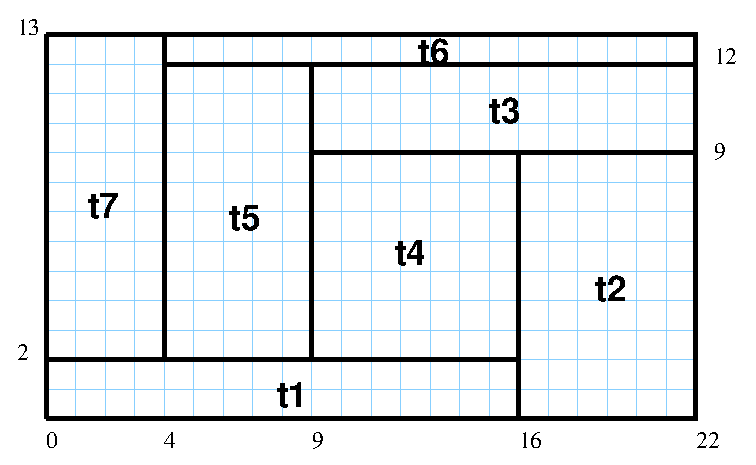
\epsfig{file=sched3.eps,width=0.45\textwidth}}

Példa precedencia-korlátra:

\begin{alltt}
| ?- _S = [S1,S2], domain(_S,0,9), S1 #< S2, {\em{}% a két külön korlát}
     serialized(_S, [4,4], []).              {\em{}% nem jól szûkít:}
        S1 in 0..8, S2 in 1..9 ? ;  no

| ?- _S = [S1,S2], domain(_S,0,9), Opts=[precedences([d(2,1,sup)],
     serialized(_S, [4,4], Opts)]). {\em{}% ^^ \(\equiv\) S1 #< S2}
        S1 in 0..5, S2 in 4..9 ? ;  no
\end{alltt}
\label{order_resource}
{\bcd{order_resource(Options, Resource)}}

Igaz, ha a \cd{Resource} által leírt feladatok elrendezhetõk valamilyen
sorrendbe. Ezeket az elrendezéseket felsorolja. A \cd{Resource} argumentumot a
fenti ütemezõ eljárásoktól kaphatjuk meg az ütemezõ eljárás opció-listájába
helyezett \cd{resource(Resource)} elemmel. Az \cd{order_resource/2} opció-listája
a következõ dolgokat tartalmazhatja (mindegyik csoportból legfeljebb egyet,
alapértelmezés: \cd{[first,est]}):

\begin{itemize}
\item stratégia
     \begin{itemize}
     \item \cd{first} Mindig olyan feladatot választunk ki, amelyet az összes
                       többi elé helyezhetünk.
     \item \cd{last} Mindig olyan feladatot választunk ki, amelyet az összes
                       többi után helyezhetünk.
     \end{itemize}
\item tulajdonság: \cd{first} stratégia esetén az adott tulajdonság
     minimumát, \cd{last} esetén a maximumát tekintjük az összes feladatra
     nézve.
     \begin{itemize}
     \item \cd{est} legkorábbi lehetséges kezdési idõ
     \item \cd{lst} legkésõbbi lehetséges kezdési idõ
     \item \cd{ect} legkorábbi lehetséges befejezési idõ
     \item \cd{lct} legkésõbbi lehetséges befejezési idõ
     \end{itemize}
\end{itemize}

Példa:

\begin{verbatim}
| ?- _S=[S1,S2,S3], domain(_S, 0, 9),
     serialized(_S, [5,2,7],
                [precedences([d(3,1,sup), d(3,2,sup)]),
                 resource(_R)]), order_resource([],_R).
S1 in 0..2, S2 in 5..7, S3 in 7..9 ? ;
S1 in 2..4, S2 in 0..2, S3 in 7..9 ? ;
no
\end{verbatim}

Látható, hogy az \cd{order_resource/2} csak a lehetséges elrendezésekre vonatkozóan
címkéz, de az egyes elrendezéseken belül a változók értékeit ,,függõben'' hagyja.

\subsubsection{Diszjunkt szakaszok és téglalapok}

{\bcd{disjoint1(Lines{\em [}, Options{\em ]})}}

Jelentése: A \cd{Lines} által megadott intervallumok diszjunktak. A \cd{Lines} lista
elemei $F(S_j,D_j)$ vagy $F(S_j,D_j,T_j)$ alakú kifejezések listája, ahol $S_j$ és
$D_j$ $j$. szakasz kezdõpontját és hosszát megadó változók. $F$ tetszõleges funktor,
$T_j$ egy atom vagy egy egész, amely a szakasz típusát definiálja (alapértelmezése 0).
Az \cd{Options} lista a következõ dolgokat tartalmazhatja (a \cd{Boolean} változók
alapértelmezése \cd{false}):

\begin{itemize}
\item \cd{decomposition(Boolean)}
          Ha \cd{Boolean} \cd{true}, akkor minden ébredéskor megpróbálja kisebb
          darabokra bontatni a korlátot.

\item \cd{global(Boolean)}
          Ha \cd{Boolean} \cd{true}, akkor egy redundáns algoritmust használ a
          jobb szûkítés érdekében. Példa:

\begin{verbatim}
| ?- domain([S1,S2,S3], 0, 9), (G = false ; G = true),
     disjoint1([S1-8,S2-2,S3-2], [global(G)]).
       G = false, S1 in 0..9, S2 in 0..9, S3 in 0..9 ? ;
       G = true,  S1 in 4..9, S2 in 0..7, S3 in 0..7 ? 
\end{verbatim}

\item \cd{wrap(Min,Max)}
          A szakaszok nem egy egyenesen, hanem egy körön helyezkednek el,
          ahol a \cd{Min} és \cd{Max} pozíciók egybeesnek (\cd{Min} and
          \cd{Max} egészek kell, hogy legyenek). Ez az opció a \cd{Min..(Max-1)}
          intervallumba kényszeríti a kezdõpontokat.

\item \cd{margin(T1,T2,D)}
          Bármely \cd{T1} típusú vonal végpontja legalább \cd{D} távolságra lesz
          bármely \cd{T2} típusú vonal kezdõpontjától, ha \cd{D} egész.
          Ha \cd{D} nem egész, akkor a \cd{sup} atomnak kell lennie, ekkor
          minden \cd{T2} típusú vonalnak elõrébb kell lennie, mint bármely
          \cd{T1} típusú vonal.
\end{itemize}

{\bcd{disjoint2(Rectangles{\em [}, Options{\em ]})}}

     Jelentése: A \cd{Rectangles} által megadott téglalapok nem metszik
     egymást. A \cd{Rectangles} lista elemei $F(S_{j1},D_{j1},S_{j2},D_{j2})$
     vagy $F(S_{j1},D_{j1},S_{j2},D_{j2},T_j)$ alakú kifejezések. Itt
     $S_{j1}$ és $D_{j1}$ a $j$. téglalap X irányú kezdõpontját és hosszát
     jelölõ változók, $S_{j2}$ és $D_{j2}$ ezek Y irányú megfelelõi,
     $F$ tetszõleges funktor,  $T_j$ egy egész vagy atom, amely a
     téglalap típusát jelöli (alapértelmezése 0).

Az \cd{Options} lista a következõ dolgokat tartalmazhatja (a \cd{Boolean} változók
alapértelmezése \cd{false}):

\begin{itemize}
\item \cd{decomposition(Boolean)}
          Mint \cd{disjoint1/2}.

\item \cd{global(Boolean)}
          Mint \cd{disjoint1/2}.

\item \cd{wrap(Min1,Max1,Min2,Max2)}
          \cd{Min1} és \cd{Max1} egész számok vagy rendre az \cd{inf} vagy
          \cd{sup} atom. Ha egészek, akkor a téglalapok egy olyan henger
          palástján helyezkednek el, amely az X irányban fordul körbe, ahol
          a \cd{Min1} és \cd{Max1} pozíciók egybeesnek. Ez az opció a
          \cd{Min1..(Max1-1)} intervallumba kényszeríti az $S_{j1}$ változókat.
          \cd{Min2} és \cd{Max2} ugyanezt jelenti Y irányban. Ha mind a négy
          paraméter egész, akkor a téglalapok egy tóruszon helyezkednek el.

\item \cd{margin(T1,T2,D1,D2)}
          Ez az opció minimális távolságokat ad meg, \cd{D1} az X,
          \cd{D2} az Y irányban bármely \cd{T1} típusú téglalap vég- és bármely \cd{T2}
          típusú téglalap kezdõpontja között. \cd{D1} és \cd{D2} egészek vagy a
          \cd{sup} atom. \cd{sup} azt jelenti, hogy a \cd{T2} típusú téglalapokat
          a \cd{T1} típusú téglalapok elé kell helyezni a megfelelõ irányban.

\item \cd{synchronization(Boolean)}:  Speciális esetben redundáns korlátot
          vesz fel (lásd SICStus kézikönyv).
\end{itemize}

Példa: helyezzünk el három diszjunkt téglalapot úgy, hogy $(x,y)$ bal alsó sarkuk
az $0 \leq x \leq 2, 0 \leq y \leq 1$ téglalapban legyen. A méretek ($x \times y$
sorrendben): 1 $\times$ 3, 2 $\times$ 2, 3 $\times$ 3. Az 1 $\times$ 3-as téglalap
$x$ koordinátája nem lehet 2.

\begin{verbatim}
| ?- domain([X1,X2,X3], 0, 2), domain([Y1,Y2,Y3], 0, 1), X1 #\= 2,
     disjoint2([r(X1,3,Y1,1),r(X2,2,Y2,2),r(X3,3,0,3)]).
X1 in 0..1, Y1 = 0,   X2 = 0, Y2 = 1,   X3 = 2, Y3 = 1 ?
\end{verbatim}

\subsection{Felhasználói korlátok definiálása}

A SICStus Prolog kétféle lehetõséget kínál a \clpfd modul korlátainak
felhasználói korlátokkal való bõvítésére: a \emph{globális korlát}okat és
az \emph{FD predikátum}okat. A \emph{globális korlát}ok tetszõleges (nem korlátos)
számú változót tartalmazó korlátok definiálására alkalmasak. A korlátok
mûködését teljesen általános Prolog kódként adhatjuk meg, beleértve az
ébresztési feltételeket és a befejezés módját is. A globális korlátok
reifikációja (tükrözése) azonban nem támogatott. Az \emph{FD predikátumok}
ezzel szemben csak rögzített számú változót tartalmazó korlátok leírására
alkalmasak, viszont itt a reifikáció is támogatott, és az ébresztési
feltételek meghatározása automatikus. Az FD predikátumokban a programozó
úgynevezett \emph{indexikálisok} segítségével írja le a szûkítési, illetve
levezethetõségi feltételeket. Az indexikálisok nyelve egy speciális, halmazértékû
funkcionális nyelv a tartományokkal való mûveletek végzésére. Az alábbi
Prolog kód egy példa egy FD predikátumra:

\begin{alltt}
% Az X+Y #= T korlát (intervallum szûkítéssel)
'x+y=t'(X,Y,T) +:  
        X in min(T) - max(Y)..max(T) - min(Y),
        Y in min(T) - max(X)..max(T) - min(X),
        T in min(X) + min(Y)..max(X) + max(Y).
\end{alltt}

Az indexikális nyelv bõvebb elemzése az \ref{fdpred}. fejezetben olvasható.

\subsubsection{Globális korlátok}

\label{globalis}

Mint azt már említettük, a globális korlátot egy külön Prolog eljárásként
kell megírni, amelyben az \cd{fd\_global/3} eljárással indul el a korlát
tényleges végrehajtása. Az \cd{fd\_global/3} paraméterezése:
\br
{\bcd{fd\_global(Constraint, State, Susp)}}\\
Elindítja \cd{Constraint} végrehajtását \cd{State} kezdõállapottal és
\cd{Susp} ébresztési feltételekkel. \cd{Constraint} egy tetszõleges Prolog
struktúra lehet, azonban célszerû a korlát nevével megegyezõre választani,
már csak azért is, mert ha a \cd{clpfd:full_answer} bekapcsolásával kérjük
a le nem futott démonok megjelenítését, akkor a Prolog a \cd{Constraint}-ben
megadott nevet fogja kiírni.
\br
A Prolog lehetõséget biztosít arra, hogy a globális korlát az ébresztések
között megõrizzen bizonyos állapotinformációkat. Ez az állapotinformáció
is tetszõleges Prolog struktúra lehet, a kezdõértékét pedig a \cd{State}
paraméterrel tudjuk beállítani.
\br
A korlát indításakor az \cd{fd\_global/3} harmadik paraméterében
meg kell adni egy ébresztési listát, amely elõírja, hogy mely változók
milyen tartomány-változásakor kell felébreszteni a korlátot. A lista elemei
a következõk lehetnek:
\begin{itemize}
\item \cd{dom(X)} --- az \cd{X} változó tartományának bármely
változásakor
\item \cd{min(X)} --- az \cd{X} változó alsó határának változásakor
\item \cd{max(X)} --- az \cd{X} változó felsõ határának változásakor
\item \cd{minmax(X)} --- az \cd{X} változó alsó vagy felsõ határának
változásakor
\item \cd{val(X)} --- az \cd{X} változó behelyettesítésekor
\end{itemize}

Fontos, hogy a korlát \emph{nem} tudja majd, hogy melyik változójának milyen
változása miatt ébresztik fel. Ráadásul ha több változás történik, a korlát
akkor is csak egyszer fog felébredni, éppen ezért nagyon fontos, hogy a
korlát minden lehetséges tartomány-változásra megfelelõen reagáljon anélkül,
hogy tudná, hogy pontosan melyik változó változása ébresztette fel õt.
\br
Az \cd{fd\_global/3} meghívásakor és minden ébredéskor a rendszer elvégzi a
felhasználó által megadott szûkítéseket. Ezeket a szûkítéseket a
\cd{clpfd:dispatch\_global/4} többállományos (\cd{multifile}) kampó-eljárás
kibõvítésével lehet megadni.
\br
{\bcd{clpfd:dispatch\_global(Constraint, State, NewState, Actions)}}\\
Ennek az eljárásnak a törzse definiálja a \cd{Constraint} korlát ébredésekor
végrehajtandó teendõket és állapot-változásokat. A \cd{Constraint} paraméterben
ugyanaz a struktúra fog megjelenni, mint amit az \cd{fd\_global/3} elsõ
paraméterében átadtunk. \cd{State} tartalmazza az ébredéskor fennálló állapotot,
\cd{NewState}-et pedig nekünk kell majd kitölteni az új állapottal. A végrehajtandó
szûkítéseket \emph{tilos} a kampó-eljárás belsejében végrehajtani, helyette ezeket
az \cd{Actions} listában kell átadnunk, és ott kell jeleznünk a korlát sikeres
lefutását vagy meghiúsulását is. Alapértelmezésben a korlát démona az eljárás
lefutása után visszaalszik.
\br
Az \cd{Actions} lista az alábbi elemekbõl állhat (a sorrend nem számít):

\begin{itemize}
\item \cd{exit} ill. \cd{fail} --- a korlát sikeresen ill. sikertelenül lefutott
\item \cd{X=V}, \cd{X in R}, \cd{X in\_set S} --- az adott szûkítést kérjük végrehajtani
(ez is okozhat meghiúsulást)
\item \cd{call(Module:Goal)} --- az adott hívást kérjük végrehajtani. A
\cd{Module:} modul-kvalifikáció kötelezõ!
\end{itemize}

Mivel a \cd{dispatch_global/4} eljárás a többi \cd{multifile} eljáráshoz hasonlóan
interpretáltan fut, ezért a futás gyorsítása érdekében célszerû a \cd{dispatch_global}
eljárások törzsébe csak egyetlen klózt írni, ami az általunk írt korlátkezelõ eljárásra
mutat (mivel az már betöltéskor le fog fordulni, és így gyorsabb lesz a futás).
\br
Az alábbi példa az \cd{X \#=< Y} korlát megvalósítása globális korlátként:

\begin{verbatim}
:- multifile clpfd:dispatch_global/4.
:- discontiguous clpfd:dispatch_global/4.   % nem folytonos eljárás

% X #=< Y, globális korlátként megvalósítva.
lseq(X, Y) :-
        % lseq(X,Y) globális démon indul, kezdõállapot: void.
        % Ébredés: X alsó és Y felsõ határának változásakor.
        fd_global(lseq(X,Y), void, [min(X),max(Y)]).

clpfd:dispatch_global(lseq(X,Y), St, St, Actions) :-
        dispatch_lseq(X, Y, Actions).

dispatch_lseq(X, Y, Actions) :-
        fd_min(X, MinX), fd_max(X, MaxX),
        fd_min(Y, MinY), fd_max(Y, MaxY),
        (   number(MaxX), number(MinY), MaxX =< MinY
            % buzgóbb, mint X#=<Y, mert az csak X vagy Y
            % behelyettesítésekor fut le.
        ->  Actions = [exit]
        ;   Actions = [X in inf..MaxY,Y in MinX..sup]
        ).
\end{verbatim}

A fenti korlát mûködése igen egyszerû. Elõször meghatározzuk \cd{X} és \cd{Y} tartományainak
szélsõ határait a megfelelõ változókba. Ezek után ha \cd{MaxX} és \cd{MinY} is szám
(tehát nem \cd{inf} vagy \cd{sup}), valamint \cd{MaxX} kisebb vagy egyenlõ, mint \cd{MinY},
akkor befejezzük a mûködésünket, ellenkezõ esetben \cd{X}-et az \cd{inf..MaxY}, \cd{Y}-t
a \cd{MinX..sup} intervallumra szûkítjük, és újra elalszunk. Ha az elõzõ két szûkítés
valamelyike meghiúsulna, akkor a Prolog automatikusan gondoskodik arról, hogy visszalépés
következzen be.
\br
Újabb példa, ezúttal az \cd{S = sign(X)} (\cd{X} elõjele \cd{S}) korlátra:

\begin{alltt}
% X elõjele S, globális korlátként megvalósítva.
sign(X, S) :-
        S in -1..1,
        fd_global(sign(X,S), void, [minmax(X),minmax(S)]).
        % Ébredés: X és S alsó és felsõ határának változásakor.

clpfd:dispatch_global(sign(X,S), St, St, Actions) :-
        fd_min(X, MinX0), sign_of(MinX0, MinS),
        fd_max(X, MaxX0), sign_of(MaxX0, MaxS),
        fd_min(S, MinS0), sign_min_max(MinS0, MinX, _),
        fd_max(S, MaxS0), sign_min_max(MaxS0, _, MaxX),
        Actions = [X in MinX..MaxX, S in MinS..MaxS|Exit],
        (   max(MinS0,MinS)=:=min(MaxS0,MaxS) -> Exit = [exit]
        ;   Exit = []
        ).

% sign_of(X, S): X egész vagy végtelen érték elõjele S
sign_of(inf, S) :- !, S = -1.
sign_of(sup, S) :- !, S = 1.
sign_of(X, S) :- S is sign(X).

% sign_min_max(S, Min, Max): \(sign(x)=\cd{S} \Leftrightarrow x \in \cd{Min..Max}\)
sign_min_max(-1, inf, -1).
sign_min_max(0, 0, 0).
sign_min_max(1, 1, sup).
\end{alltt}

A reifikáció megvalósítása globális korláttal:

\begin{verbatim}
% X #=< Y #<=> B, globális korlátként megvalósítva.
lseq_reif(X, Y, B) :-
        B in 0..1, fd_global(lseq_reif(X,Y,B), void,       
                             [minmax(X),minmax(Y),val(B)]).

clpfd:dispatch_global(lseq_reif(X,Y, B), St, St, Actions) :-
        fd_min(X, MinX), fd_max(X, MaxX),
        fd_min(Y, MinY), fd_max(Y, MaxY),
        (   fdset_interval(_, MaxX, MinY)   % MaxX =< MinY
        ->  Actions = [exit,B=1]  
        ;   empty_interval(MinX, MaxY)      % MaxY < MinX
        ->  Actions = [exit,B=0]
        ;   B == 1 -> Actions = [exit, call(user:lseq(X,Y))]
        ;   B == 0 -> Actions = [exit, call(user:less(Y,X))]
        ;   Actions = []
        ).
\end{verbatim}

Ehhez hasonló trükkökkel természetesen tetszõleges globális korlátot átírhatunk
olyan alakba, amely egy 0-1 értékû változóban tükrözi az igazságértékét, de
ez nem ,,tiszta'' reifikáció. Mindössze annyi ilyenkor a teendõnk, hogy meghatározzuk
azokat a feltételeket, amelyekbõl kiderül, hogy a korlát, illetve a negáltja levezethetõ,
és ezen feltételek teljesülése esetén az igazságértéket \cd{0}-ra, illetve \cd{1}-re
kell szûkítenünk. Ugyanakkor arra is figyelni kell, hogy ha az igazságérték kerül
behelyettesítésre, akkor a korlátot, illetve a negáltját ezúttal reifikáció nélkül
kell felvennünk a tárba.
\br
Valósítsuk meg globális korlátként a mágikus sorozatok példájában már használt
\cd{pontosan/3} korlátot! (Emlékeztetõül: \cd{pontosan(I, L, E)} $\Leftrightarrow$
az \cd{I} elem \cd{L}-ben \cd{E}-szer fordul elõ)

\begin{alltt}
% Az Xs listában az I szám pontosan N-szer fordul elõ.
% N és az Xs lista elemei FD változók vagy számok lehetnek.
exactly(I, Xs, N) :-
    dom_susps(Xs, Susp),
    length(Xs, Len), N in 0..Len,
    fd_global(exactly(I,Xs,N), Xs/0, [minmax(N)|Susp]).
    % Állapot: L/Min ahol L az Xs-bõl az I-vel azonos ill.
    % biztosan nem-egyenlõ elemek esetleges kiszûrésével áll
    % elõ, és Min a kiszûrt I-k száma.

% dom_susps(Xs, Susp): Susp dom(X)-ek listája, minden X \(\in\) Xs-re.
dom_susps([], []).
dom_susps([X|Xs], [dom(X)|Susp]) :- 
    dom_susps(Xs, Susp).

clpfd:dispatch_global(exactly(I,_,N), Xs0/Min0, Xs/Min, Actions) :-
    ex_filter(Xs0, Xs, Min0, Min, I),
    length(Xs, Len), Max is Min+Len,
    fd_min(N, MinN), fd_max(N, MaxN),
    (   MaxN =:= Min -> Actions = [exit,N=MaxN|Ps],
        ex_neq(Xs, I, Ps)            % Ps = \(\{x\) in_set \bs\{I\}\( | x\in\) Xs\(\}\)
    ;   MinN =:= Max -> Actions = [exit,N=MinN|Ps],
        ex_eq(Xs, I, Ps)             % Ps = \(\{x\) in_set  \{I\}\( | x\in\) Xs\(\}\)
    ;   Actions = [N in Min..Max]
    ).

% ex_filter(Xs, Ys, N0, N, I): Xs-bõl az I-vel azonos ill. attól
% biztosan különbözõ elemek elhagyásával kapjuk Ys-t,
% N-N0 a kiszûrt I-k száma.
ex_filter([], [], N, N, _).
ex_filter([X|Xs], Ys, N0, N, I) :-
    X==I, !, N1 is N0+1, ex_filter(Xs, Ys, N1, N, I).
ex_filter([X|Xs], Ys0, N0, N, I) :-
    fd_set(X, Set), fdset_member(I, Set), !,   % X még lehet I
    Ys0 = [X|Ys], ex_filter(Xs, Ys, N0, N, I).
ex_filter([_X|Xs], Ys, N0, N, I) :-            % X már nem lehet I
    ex_filter(Xs, Ys, N0, N, I).

% A Ps lista elemei `X in_set S', \(\forall\) X \(\in\) Xs-re, S az \bs\{I\} FD halmaz.
ex_neq(Xs, I, Ps) :- 
    fdset_singleton(Set0, I), fdset_complement(Set0, Set), 
    eq_all(Xs, Set, Ps).

% A Ps lista elemei `X in_set S', \(\forall\) X \(\in\) Xs-re, S az \{I\} FD halmaz.
ex_eq(Xs, I, Ps) :- 
    fdset_singleton(Set, I), eq_all(Xs, Set, Ps).

% eq_all(Xs, S, Ps): Ps `X in_set S'-ek listája, minden X \(\in\) Xs-re.
eq_all([], _, []).
eq_all([X|Xs], Set, [X in_set Set|Ps]) :- 
    eq_all(Xs, Set, Ps).


| ?- exactly(5, [A,B,C], N), N #=< 1, A=5.
A = 5, B in (inf..4)\bs/(6..sup), C in (inf..4)\bs/(6..sup), N = 1 ?
| ?- exactly(5, [A,B,C], N), A in 1..2, B in 3..4, N #>= 1.
A in 1..2, B in 3..4, C = 5, N = 1 ?
| ?- _L=[A,B,C], domain(_L,1,3), A #=< B, B #< C, exactly(3, _L, N).
A in 1..2, B in 1..2, C in 2..3, N in 0..1 ?
\end{alltt}

A SICStus 3.8.6-nál és a régebbi verzióknál a fenti megvalósítás kapcsán egy érdekes
hibával találhatjuk magunkat szemközt:

\begin{verbatim}
| ?- L = [N,1], N in {0,2}, exactly(0, L, N).
L = [0,1], N = 0 ? ;
no
\end{verbatim}

Amint látható, a kapott megoldás hibás, hiszen a \cd{[0,1]} listában a \cd{0} elem
nem 0-szor fordul elõ, tehát az \cd{exactly(0, L, N)} korlát nem áll fenn. A probléma
általánosan a következõképpen fogalmazható meg:

\begin{quote}
Legyen \cd{c(X,Y)} egy globális korlát, amely \cd{[dom(X),dom(Y)]}
ébresztésû. Tegyük fel, hogy \cd{X} tartománya változik, és ennek hatására
a korlát szûkíti \cd{Y} tartományát. Kérdés: ébredjen-e fel ettõl újra a
korlát?
\end{quote}

A SICStus fejlesztõi úgy döntöttek, hogy ilyen esetben a korlát ne ébredjen fel újra.
Emiatt egy globális korláttal szemben támasztanunk kell egy olyan elvárást, hogy az
\emph{idempotens} legyen: ha meghívjuk, elvégezzük az akció-lista feldolgozását,
majd azonnal újra meghívjuk, akkor a második hívás már biztosan ne váltson ki további
szûkítéseket (tehát ne legyen érdemes újra meghívni). Formálisan: $dg(dg(s))=dg(s)$,
ahol $dg$ a \cd{dispatch_global/4} eljárásnak a tárra gyakorolt hatását jelöli.
\br
Jelen példánkban a korlátunk megvalósítása nem teljesíti az idempotencia feltételét,
mivel az \cd{L} lista elsõ eleme \cd{N}, és ezáltal \cd{N}-en keresztül az \cd{exactly/3}
második és harmadik paramétere ,,össze van kapcsolva''. A SICStus a 3.8.7. verzió óta
figyeli az összekapcsolt változókat, és ha ilyet talál, akkor automatikusan feltételezi
a $dg$ függvényrõl, hogy az nem idempotens, ezért újra és újra meghívja az \cd{exactly/3}
korlát démonát egészen addig, amíg van szûkítés. Így a második meghívás alkalmával
már kiderül a fent megtalált megoldásról, hogy az hibás.

\subsubsection{FD predikátumok}

\label{fdpred}

Az FD predikátumok segítségével egy korlát levezethetõségi és szûkítési szabályait
írhatjuk le egy halmazértékû funkcionális nyelv alkalmazásával. Egy FD predikátum
formailag hasonlít egy hagyományos Prolog predikátumhoz, de más a jelentése, és
szigorúbb formai szabályokkal is szembe kell néznünk.
\br
Az FD predikátumok mindig 1..4 klózból állnak, és mindnek más a ,,nyakjele''. A
\cd{+:} nyakjelû klózt kötelezõ megírni, a \cd{-:}, \cd{+?} és \cd{-?} nyakjelûek
opcionálisak, akkor van rájuk szükség, ha reifikálható korlátot szeretnénk írni.
A klózok törzse úgynevezett \emph{indexikális}ok gyûjteményébõl áll, az egyes
indexikálisokat vesszõvel kell egymástól elválasztani, de ez esetben a vesszõ
\emph{nem} konjunkciót jelent, a hagyományos Prolog predikátumokkal ellentétben.
A \cd{+:} és \cd{-:} nyakjelû klózok \emph{szûkítõ} (\emph{mondó}, \emph{tell})
indexikálisokból állnak, és azt írják le, hogy az adott korlát, illetve a negáltja
hogyan szûkíti a korlát-tárat. A \cd{+?} és \cd{-?} nyakjelû klózok egyetlen
\emph{kérdezõ} (\emph{ask}) indexikálist tartalmaznak, amely azt írja le, hogy
a korlát, illetve a negáltja mely feltétel teljesülése esetén vezethetõ le a
tárból. Az FD klózok fejében az argumentumok kötelezõen csak változók lehetnek,
és a törzsben is csak ezek a változók szerepelhetnek. Példaként tekintsük az
\cd{X \#=< Y} korlát FD predikátum változatát:

\begin{verbatim}
'x=<y'(X,Y) +:                 % Az X =< Y korlát szûkítései.
        X in inf..max(Y),      % X szûkítendõ az inf..max(Y),
        Y in min(X)..sup.      % Y a min(X)..sup intervallumra.

'x=<y'(X,Y) -:                 % Az X =< Y korlát negáltjának,
        X in (min(Y)+1)..sup,  % azaz az X > Y korlátnak a
        Y in inf..(max(X)-1).  % szûkítései.

'x=<y'(X,Y) +?                 % Ha X tartománya része az 
        X in inf..min(Y).      % inf..min(Y) intervallumnak, 
                               % akkor X =< Y levezethetõ.

'x=<y'(X,Y) -?                 % Ha X tartománya része a 
        X in (max(Y)+1)..sup.  % (max(Y)+1)..sup intervallumnak, 
                               % akkor X > Y levezethetõ.
\end{verbatim}

A fenti példából már láthatjuk, hogy az összes indexikális \cd{{\em Változó} in {\em
TKif}} alakú, ahol a \cd{{\em TKif}} tartománykifejezés tartalmazza a
\cd{{\em Változó}}-tól különbözõ \emph{összes} fejváltozót. Ha olyan indexikálist
írunk, amelyre ez utóbbi feltétel nem teljesül, akkor igen nagy a valószínûsége,
hogy az indexikális hibásan fog mûködni (erre a \pageref{hibas_indexikalis}. oldalon
látunk is majd egy példát). A \cd{\em{TKif}} tartománykifejezés (\emph{range})
egy (parciális) halmazfüggvényt ír le, azaz a benne szereplõ változók tartományának
függvényében egy újabb tartományt állít elõ. Például a \cd{min(X)..sup} kifejezés
az \cd{X} alsó határának függvényében állít elõ egy tartományt, ha \cd{X}-rõl azt
tudjuk, hogy az \cd{1..10} intervallumban van benne, akkor \cd{min(X)..sup} = \cd{1..sup}
fog teljesülni. A \cd{{\em Változó} in {\em TKif}} alakú kifejezés \cd{\em Változó}
értékét a \cd{\em TKif} tartománykifejezés által elõállított halmazra szûkíti (bizonyos
feltételek fennállása esetén, ld. késõbb). 

Formálisan: az \cd{X in {\em R}(Y,Z,\ldots)} indexikális jelentése a következõ
reláció:

\[
Rel(R) =  \{ \tuple{x,y,z, \ldots} | x \in \parbox{0.6em}{\tt\em R}(\{y\},\{z\}, \ldots)\}
\]

Más szóval ha az \cd{\em R}-beli változóknak egyelemû a tartománya, akkor az
\cd{\em R} tartománykifejezés értéke \emph{pontosan} az adott relációt kielégítõ \cd{X}
értékek halmaza lesz (ld. még a pont-szûkítés definícióját, \pageref{pontszukites}. oldal).
\br
{\bf Az FD predikátumok alapszabálya:} az egy FD-klózon belül lévõ indexikálisok
jelentésének (azaz az általuk definiált relációnak) azonosnak kell lennie! Ennek oka
az úgynevezett ,,\emph{társasház-elv}'': az FD predikátum kiértékelésére a Prolog
\emph{bármelyik} indexikálist felhasználhatja! Gyakorlásképp nézzük meg, hogy az elõzõ
példa FD-klózaiban teljesül-e ez az alapszabály:

\begin{alltt}
'x=<y'(X, Y) +: 
    X in inf..max(Y), % \(\{\tuple{x,y}|x\in{}\cd{inf..max(\{}y\cd{\})}\} \equiv \{\tuple{x,y}|x\in{}(-\infty,y]\} \equiv \{\tuple{x,y}|x\leq{}y\}\)
    Y in min(X)..sup. % \(\{\tuple{x,y}|y\in{}\cd{min(\{}x\cd{\})..sup}\} \equiv \{\tuple{x,y}|y\in{}[x,+\infty)\} \equiv \{\tuple{x,y}|y\geq{}x\}\)
\end{alltt}

Mivel $x \leq y$ és $y \geq x$ ekvivalensek, ezért itt a társasház-elv teljesül.
\br
Most definiálni fogjuk a tartománykifejezések pontos szintaktikáját. Bevezetjük az
alábbi jelöléseket ($s$ továbbra is egy adott korlát-tárat fog jelenteni):

\begin{description}
\item[$X$] egy korlát-változó, tartománya \domx{X}. \vspace*{-1ex}
\item[$T$] egy számkifejezés ({\em term}), amelynek jelentése 
egy egész szám vagy egy végtelen érték, ezt \valx{T}-sel jelöljük. 
(Végtelen érték csak \cd{$T_1$..$T_2$}-ben lehet.) \vspace*{-1ex}
\item[$R$] egy tartománykifejezés ({\em range}), amelynek jelentése
egy számhalmaz, amit \setx{R}-sel jelölünk.
\end{description}

A tartománykifejezéseket alkotó elemi kifejezések és operátorok összefoglalva az
alábbi táblázatban láthatóak:

\begin{center}{\tt
\begin{tabular}{|p{15em}|@{\hspace*{3.5em}}p{21.5em}|}
\hline
{\rm\bf Szintaxis}                &   \hspace*{-3em}{\rm\bf Szemantika}            \\
\hline
\rule{0ex}{3ex}$T$ $\Longrightarrow$             &   \hspace*{-3em}\valx{T} =     \\
\ \ \ \ \ \ {\em integer}         &   {\em integer} {\rm értéke}                  \\
\ \ |\ \ \ inf                    &   \(-\infty\)                                 \\
\ \ |\ \ \ sup                    &   \(+\infty\)                                 \\
\ \ |\ \ \ $X$                    &   {\rm \(x\) feltéve, hogy \domx{X}\(=\{x\}\).  
                                      Egyébként az indexikális felfüggesztõdik       
                                      (,,pucér'' változó esete).}                 \\
\ \ |\ \ \ card($X$)              &   $\left| \domxm{X} \right|$ {\rm(a tartomány elemszáma)}\\
\ \ |\ \ \ min($X$)               &   \(\min(\domxm{X})\) {\rm(a tartomány alsó határa)} \\
\ \ |\ \ \ max($X$)               &   \(\max(\domxm{X})\) {\rm(a tartomány felsõ határa)} \\
\ \ |\ \ \ $T_1$ + $T_2$          &   $\valxm{T_1} + \valxm{T_2}$ \\
\ \ |\ \ \ $T_1$ - $T_2$          &   $\valxm{T_1} - \valxm{T_2}$ \\
\ \ |\ \ \ $T_1$ * $T_2$          &   $\valxm{T_1} * \valxm{T_2}$ \\
\ \ |\ \ \ $T_1$ mod $T_2$        &   $\valxm{T_1} \bmod \valxm{T_2}$             \\
\ \ |\ \ \ - $T_1$                &   $- \valxm{T_1}$ \\
\ \ |\ \ \ $T_1$ /> $T_2$         &   $\left\lceil\valxm{T_1}/\valxm{T_2}\right\rceil$
                                      {\rm (felfelé kerekített osztás)}\\
\ \ |\ \ \ $T_1$ /< $T_2$         &   $\left\lfloor\valxm{T_1}/\valxm{T_2}\right\rfloor$
                                      {\rm (lefelé kerekített osztás)}\\[1ex]
\hline
\rule{0ex}{3ex}$R$ $\Longrightarrow$  &   \hspace*{-3em}\setx{R} =                \\%[1ex]
\ \ \ \ \ \ \{$T_1$,$\ldots$,$T_n$\}   &   $\{\valxm{T_1},\ldots,\valxm{T_n}\}$    \\
\ \ |\ \ \ dom($X$)               &   \domx{X}                                     \\
\ \ |\ \ \ $T_1$..$T_2$           &   $[\valxm{T_1},\valxm{T_2}]$ 
                                      {\rm (intervallum)}           \\
\ \ |\ \ \ $R_1$/\bs{}$R_2$       &   $\setxm{R_1}\cap\setxm{R_2}$  {\rm (metszet)}\\
\ \ |\ \ \ $R_1$\bs/{}$R_2$       &   $\setxm{R_1}\cup\setxm{R_2}$  {\rm (unió)}\\
\ \ |\ \ \ \bs{}$R_1$             &   $\setminus\setxm{R_1}$   {\rm (komplementer halmaz) }                  \\
\ \ |\ \ \ - $R_1$                &   $\{ -x | x \in \setxm{R_1} \}$ {\rm (pontonkénti negáció) }                    \\
\ \ |\ \ \ $R_1$ + $R_2$          &   $\{ x+y | x \in \setxm{R_1}, y \in \setxm{R_2} \}$ {\rm (pont. összeg)}                \\                                     
\ \ |\ \ \ $R_1$ + $T_2$          &   $\{ x+t | x \in \setxm{R_1}, t = \valxm{T_2} \}$ \\
\ \ |\ \ \ $R_1$ - $R_2$          &   $\{ x-y | x \in \setxm{R_1}, y \in \setxm{R_2} \}$ {\rm (p. különbség)}                \\                                     
\ \ |\ \ \ $R_1$ - $T_2$          &   $\{ x-t | x \in \setxm{R_1}, t = \valxm{T_2} \}$ \\
\ \ |\ \ \ $T_1$ - $R_2$          &   $\{ t-y | t = \valxm{T_1}, y \in \setxm{R_2} \}$ \\
\ \ |\ \ \ $R_1$ mod $R_2$        &   $\{ x \bmod y | x \in \setxm{R_1}, y \in \setxm{R_2} \}$ {\rm (p. modulo)}                     \\                                     
\ \ |\ \ \ $R_1$ mod $T_2$        &   $\{ x \bmod t | x \in \setxm{R_1}, t = \valxm{T_2} \}$ \\
\ \ |\ \ \ unionof($X$,$R_1$,$R_2$) &   {\rm unió-kifejezés, ld. \pageref{unio:ind}. oldal }                          \\
\ \ |\ \ \ switch($T$,$MapList$)   &   {\rm kapcsoló-kifejezés, ld. \pageref{kapcs:ind}. oldal}                      \\
\ \ |\ \ \ $R_1$\ ?\ $R_2$          &   {\rm feltételes kifejezés, ld. \pageref{felt:ind}. oldal }              \\[1ex]
\hline
\end{tabular}
}\end{center}

Az ilyen kifejezésekben szereplõ összeadás, kivonás, szorzás, osztás, modulus és
ellentett mûveletek mindegyike \emph{pontonkénti} mûveletvégzés. Ez azt takarja,
hogy a mûveletet végrehajtjuk a két operandusból a Descartes-szorzat segítségével
kapott párokra, majd az eredményekbõl egy újabb halmazt képezünk. Például vegyük
az alábbi korlátot:

\begin{alltt}
f(X,Y) +: Y in 5 - dom(X).  {\em%} \(\{ \makebox[2em]{5-x} | \makebox[0.8em]{x}\in{}\cd{dom(X)} \}\) 
\end{alltt}

A fenti korlát az \cd{Y \#= 5-X} relációt valósítja meg, tartományszûkítõ módon:

\begin{verbatim}
| ?- X in {1, 3, 5}, f(X,Y).
Y in{0}\/{2}\/{4} ?
\end{verbatim}

Itt a korlát belsejében az \cd{Y in 5 - dom(X)} hívás során minden $x \in$ \domx{X}-re
végrehajtódik az $y = 5-x$ kivonás, majd ezeket az $y$-okat egy halmazba rakva kapjuk
\domx{Y}-t.
\br
A korábban \cd{plusz/3} néven hivatkozott tartományszûkítõ összegkorlát FD predikátummal
való megvalósítása:

\begin{alltt}
| 'x+y=t tsz'(X, Y, T) +:
        X in dom(T) - dom(Y), {\em%} \(\{ \makebox[2em]{t-y} | \makebox[0.8em]{t}\in{}\cd{dom(T)}, \makebox[0.8em]{y}\in{}\cd{dom(Y)} \}\) 
        Y in dom(T) - dom(X), {\em%} \(\{ \makebox[2em]{t-y} | \makebox[0.8em]{t}\in{}\cd{dom(T)}, \makebox[0.8em]{x}\in{}\cd{dom(X)} \}\) 
        T in dom(X) + dom(Y). {\em%} \(\{ \makebox[2em]{x+y} | \makebox[0.8em]{x}\in{}\cd{dom(X)}, \makebox[0.8em]{y}\in{}\cd{dom(Y)} \}\) 

| ?- _X in \{10,20\}, _Y in \{0,5\}, _X+_Y #= Z.
Z in 10..25 ?
| ?- _X in \{10,20\}, _Y in \{0,5\}, 'x+y=t tsz'(_X, _Y, Z).
Z in\{10\}\bs/\{15\}\bs/\{20\}\bs/\{25\} ?
\end{alltt}

Példa ,,pucér'' (indexikálisban önmagában álló) változóra:

\begin{alltt}
f(X,Y,I) +: Y in \bs\{X,X+I,X-I\}.
% hasonló az N királynõ feladat no_threat/3 korlátjához, ld. \pageref{no:threat}. oldal

| ?- X in \{3, 5\}, Y in 1..5, f(X, Y, 2), X = 3.
Y in \{2\}\bs\{4\} ?
\end{alltt}

Pucér változó használata esetén az indexikális végrehajtása felfüggesztõdik addig,
amíg a pucér változók be nem helyettesítõdnek. Végül egy példa bonyolultabb számkifejezés
indexikálisos megvalósítására:

\begin{alltt}
| 'ax+c=t'(A,X,C,T) +:  % feltétel: A > 0
        X in (min(T) - C) /> A .. (max(T) - C) /< A,
        T in min(X)*A + C      ..  max(X)*A + C.

| ?- 'ax+c=t'(2,X,1,T), T in 0..4.
X in 0..1, T in 1..3 ?
\end{alltt}

\subsubsection{Indexikálisok monotonitása}

Az imént említettük azt is, hogy a \cd{{\em Változó} in {\em TKif}} alakú indexikális
\cd{\em Változó} értékét csak bizonyos feltételek teljesülése mellett szûkíti
a \cd{\em TKif} tartománykifejezés által elõállított halmazra. Most tisztázni fogjuk,
hogy mik is ezek a bizonyos feltételek. Tekintsük az alábbi két FD predikátumot:

\begin{alltt}
f(X, Y) +: Y in min(X)..sup.

| ?- X in 5..10, f(X, Y).
X in 5..10, Y in 5..sup?

f(X, Y) +: Y in max(X)..sup.

| ?- X in 5..10, f(X, Y).
X in 5..10, Y in inf..sup?
\end{alltt}

A két FD predikátum ránézésre nagyjából megegyezik, ha \cd{X} tartománya egyelemû
lenne, akkor mindkettõ az \cd{Y \#>= X} korláttal ekvivalens jelentésû lenne. A második
esetben azonban a Prolog mégsem hajlandó szûkíteni, ugyanis az \cd{Y in 10..sup}
szûkítést kéne végrehajtania, majd \cd{X} tartományának késõbbi szûkülésekor \cd{Y}
tartományát \emph{bõvítenie} kellene, ami nem lehetséges. Például ha a késõbbiekben
kiderülne, hogy \cd{X in 6..7}, akkor \cd{Y}-nak a \cd{7..sup} tartományra kéne
bõvülnie.
\br
Az általános megfogalmazáshoz vezessünk be néhány újabb fogalmat:
\br
\definicio egy $R$ tartománykifejezés egy $s$ tárban \emph{kiértékelhetõ}, ha az
$R$-ben elõforduló összes ,,pucér'' változó tartománya az $s$ tárban
egyelemû (be van helyettesítve). A továbbiakban csak kiértékelhetõ
tartománykifejezésekkel foglalkozunk.
\br
\definicio egy $s$ tárnak \emph{pontosítás}a $s'$ ($s' \subseteq s$), ha minden
$X$ változóra $D(X,s') \subseteq D(X,s)$ (azaz $s'$ szûkítéssel állhat elõ $s$-bõl).
\br
\definicio egy $R$ tartománykifejezés egy $s$ tárra nézve \emph{monoton}, ha
minden $s' \subseteq s$ esetén $S(R,s') \subseteq S(R,s)$, azaz a tár
szûkítésekor a kifejezés értéke is szûkül.
\br
\definicio egy $R$ tartománykifejezés egy $s$ tárra nézve \emph{antimonoton}, ha
minden $s' \subseteq s$ esetén $S(R,s') \supseteq S(R,s)$.
\br
\definicio $R$ $s$-ben konstans, ha monoton és antimonoton (azaz $s$ szûkülésekor
már nem változik).
\br
\definicio egy indexikálist monotonnak, antimonotonnak, ill. konstansnak nevezünk,
ha a tartománykifejezése monoton, antimonoton, ill. konstans. 

\enum{Példák}{
\item \cd{min(X)..max(Y)} egy tetszõleges tárban monoton.
\item \cd{max(X)..max(Y)} monoton minden olyan tárban, ahol \cd{X} behelyettesített,
és antimonoton, ahol \cd{Y} behelyettesített.
\item \cd{card(X)..Y} kiértékelhetõ, ha \cd{Y} behelyettesített, és ilyenkor antimonoton.
\item \cd{(min(X)..sup) \bs/ (0..sup)} egy tetszõleges tárban monoton,
és konstans minden olyan tárban, ahol \cd{min(X) >= 0}.
}

\tetel ha egy ,,\cd{$X$ in $R$}'' indexikális monoton egy $s$ tárban, akkor
$X$ értéktartománya az $S(R,s)$ tartománnyal szûkíthetõ.
\br
{\bf Bizonyítás} (vázlat): Tegyük fel, hogy $x_0 \in D(X,s)$ egy tetszõleges olyan
érték, amelyhez találhatók olyan $y_0 \in D(Y,s$), $z_0 \in D(Z,s)$, \ldots értékek, hogy 
$\tuple{x_0,y_0,z_0,\ldots}$ kielégíti az indexikális által definiált relációt. Azaz

\[ \tuple{x_0,y_0,z_0,\ldots} \in Rel(R) \Leftrightarrow x_0 \in S(R, s'), 
s'= \{Y~\cd{in}~\{y_0\},Z~\cd{in}~\{z_0\},\ldots\} \]

Itt $s' \subseteq s$, hiszen $y_0 \in D(Y,s$), $z_0 \in D(Z,s)$,
\ldots. A monotonitás miatt $S(R, s)
\supseteq S(R, s') \ni x_0$. Így tehát $S(R, s)$ tartalmazza az összes, a
reláció által az $s$ tárban megengedett értéket, ezért ezzel a halmazzal
való szûkítés jogos.
\br
A \clpfd rendszer egy indexikálisról a következõ irányelvek alapján dönti el, hogy
az monoton-e vagy sem:

\begin{itemize}
\item Egy számkifejezésrõl egyszerûen megállapítható, hogy a tár
szûkülésekor nõ, csökken, vagy konstans-e (kivéve \cd{$T_1$ mod $T_2$}, itt
várunk, míg $T_2$ konstans lesz).
\item Tartománykifejezések esetén:
\begin{itemize}
\item \cd{$T_1$..$T_2$} monoton, ha $T_1$ csökken és $T_2$ nõ, antimonoton,
 ha $T_1$ nõ és $T_2$ csökken.
\item \cd{dom($X$)} mindig monoton.
\item A metszet és unió mûveletek eredménye (anti)monoton, ha mindkét
operandusuk az, a komplemensképzés mûvelete megfordítja a monotonitást.
\item A pontonként végzett mûveletek megõrzik az (anti)monotonitást (ehhez a
$T_i$ operandus konstans kell legyen, pl.\ \cd{dom(X)+card(Y)}$\leadsto$\cd{dom(X)+1}).
\end{itemize}
\item Az (anti)monotonitás eldöntésekor a rendszer csak a változók behelyettesítettségét
vizsgálja, pl. a \cd{(min(X)..sup) \bs/ (0..sup)} kifejezést csak akkor tekinti
konstansnak, ha \cd{X} behelyettesített.
\end{itemize}

\subsubsection{Szûkítõ indexikálisok feldolgozási lépései}

Egy \cd{X in R} szûkítõ indexikális feldolgozása mindig a végrehajthatóság vizsgálatával
kezdõdik: ha \cd{R}-ben behelyettesítetlen (,,pucér'') változó van, vagy \cd{R}-rõl a
rendszer nem látja azonnal, hogy monoton, akkor felfüggeszti a végrehajtását addig, amíg
ezek a feltételek nem teljesülnek. Ezek után meghatározza az indexikálisból képzõdõ démon
aktiválási feltételeit az egyes \cd{R}-beli változókra nézve, mégpedig az alábbiak
szerint (\cd{Y} az \cd{R}-ben elõforduló változók egyike):

\begin{itemize}
        \item \cd{dom(Y), card(Y)} környezetben elõforduló \cd{Y} változó esetén az
        indexikális a változó tartományának bármilyen módosulásakor
        aktiválandó; 
        \item \cd{min(Y)} környezetben -- alsó határ változásakor
        aktiválandó;
         \item
        \cd{max(Y)} környezetben-- felsõ határ változásakor aktiválandó.
\end{itemize}

A szûkítés menete a következõek szerint történik: ha $D(X,s)$ és $S(R,s)$ diszjunktak,
akkor visszalépés következik be, egyébként a tárat az $X\ \cd{in}\ S(R,s)$ korláttal
szûkítjük (erõsítjük), azaz $D(X,s):= D(X,s) \cap S(R,s)$. A démon akkor fejezi be
mûködését, ha az \cd{R} tartománykifejezés konstanssá válik (például azért, mert
minden \cd{R}-beli változó behelyettesítõdik). Ekkor $Rel(\cd{R})$ garantáltan fennáll,
ezért \emph{az indexikálist tartalmazó korlát} levezethetõ, ilyenkor viszont a társasház-elv
alapján hatékonysági okokból a korlát \emph{összes} indexikálisa befejezi a mûködését.
\br
Az indexikálisok feldolgozási lépéseit néhány példán keresztül is bemutatjuk:

\begin{alltt}
'x=<y'(X, Y) +:
        X in inf..max(Y),     {\em{}% (ind1)}
        Y in min(X)..sup.     {\em{}% (ind2)}
\end{alltt}

\enum{Az \cd{\em (ind1)} indexikális végrehajtási lépései}{
\item Végrehajthatóság vizsgálata: nincs benne pucér változó, monoton, tehát végrehajtható
\item Aktiválás: \cd{Y} felsõ határának változásakor.
\item Szûkítés: \cd{X} tartományát elmetsszük az \cd{inf..max(Y)}
        tartománnyal, azaz \cd{X} felsõ határát az \cd{Y}-éra állítjuk,
        ha az utóbbi a kisebb.
\item Befejezés: amikor \cd{Y} behelyettesítõdik, akkor \cd{\em (ind1)}
        konstanssá válik. Ekkor {\bf mindkét} indexikális --- \cd{\em (ind1)}
        és \cd{\em (ind2)} is ---befejezi mûködését.  }

Egy másik korlát, kicsit kevésbé részletesen:

\begin{alltt}
'abs(x-y)>=c'(X, Y, C) +:
        X in (inf .. max(Y)-C) \bs/ (min(Y)+C .. sup),
        % vagy:  X in \bs (max(Y)-C+1 .. min(Y)+C-1),
        Y in (inf .. max(X)-C) \bs/ (min(X)+C .. sup).

| ?- 'abs(x-y)>=c'(X,Y,5), X in 0..6.
X in 0..6, Y in(inf..1)\bs/(5..sup) ?
| ?- 'abs(x-y)>=c'(X,Y,5), X in 0..9.
X in 0..9, Y in inf..sup ?
\end{alltt}

A \cd{no_threat/3} korlát (ld. N királynõ feladat, \pageref{no:threat}. oldal) kicsit
erõsebb indexikálisos megvalósítása:

\begin{alltt}
no_threat_2(X, Y, I) +:
        X in \bs\{Y,Y+I,Y-I\}, Y in \bs\{X,X+I,X-I\}.

| ?- no_threat_2(X, Y, 2), Y in 1..5, X=3.
X = 3, Y in \{2\}\bs/\{4\} ?
| ?- no_threat_2(X, Y, 2), Y in 1..5, X in \{3,5\}.
X in\{3\}\bs/\{5\}, Y in 1..5 ?
\end{alltt}

Érdemes megfigyelni, hogy a második példában nincs szûkítés annak ellenére, hogy \cd{Y}
sem 3, sem 5 nem lehet. Azonban mivel az \cd{Y}-hoz tartozó indexikálisban \cd{X}
pucéron szerepel, de még nem teljesen behelyettesített, ezért a teljes indexikális
felfüggesztõdik.
\br
Végül nézzünk egy példát arra az esetre, amikor a társasház-elv nem érvényesül, és
ezért az FD predikátum hibásan mûködik:

\label{hibas_indexikalis}
\begin{alltt}
'x=<y=<z rossz'(X, Y, Z) +:
        Y in min(X)..max(Z),    {\em%} \(\{ \tuple{x,y,z} | x \leq y \leq z\}\)
        Z in min(Y).. sup,      {\em%} \(\{ \tuple{x,y,z} |      y \leq z\}\)
        X in inf..max(Y).       {\em%} \(\{ \tuple{x,y,z} | x \leq y     \}\)

| ?- 'x=<y=<z rossz'(15, 5, Z).
Z in 5..sup ?
\end{alltt}

A korlát felvételekor egyedül a második indexikális tud aktiválódni (mivel \cd{Y} és \cd{X}
már eleve konstans), és ez leszûkíti \cd{Z}-t az \cd{5..sup} intervallumra anélkül, hogy
figyelembe venné, hogy a korlát a \cd{15} $\not\leq$ \cd{5} feltétel miatt eleve nem állhat
fenn. A javításhoz meg kell ismerkednünk azzal a három tartománykifejezéssel is, amelyekrõl
eddig még nem esett szó.

\subsubsection{Bonyolultabb tartománykifejezések}

\label{unio:ind}
\enumhead{Unió-kifejezés: \cd{unionof(X, H, T)}}

Egy \cd{unionof(X, H, T)} kifejezésben \cd{X} változó, \cd{H} és \cd{T}
tartománykifejezések. Kiértékelése egy $s$ tárban: legyen \cd{H} értéke
az $s$ tárban $S(\cd{H},s) = \{x_1, \ldots, x_n\}$ (ha $S(H,s)$ végtelen,
a kiértékelést felfüggesztjük). Képezzük a $T_i$ kifejezéseket úgy, hogy
\cd{T}-ben \cd{X} helyébe $x_i$-t írjuk. Ekkor az unió-kifejezés értéke
a $S(T_1,s), \ldots, S(T_n,s)$ halmazok uniója. Képlettel:
\[
        S(\cd{unionof(X,H,T)}, s) = \bigcup \{S(\cd{T}, (s \wedge \cd{X =}
        x)) | x \in D(\cd{H}, s)\}
\]

Egy unió-kifejezés kiértékelésének ideje/tárigénye arányos a \cd{H}
tartomány méretével!
\br
A \cd{no_threat/3} (ld. N királynõ feladat, \pageref{no:threat}. oldal) maximálisan
szûkítõ, de egyáltalán nem hatékony megvalósítása:

\begin{alltt}
no_threat_3(X, Y, I) +:
        X in unionof(B, dom(Y), \bs\{B,B+I,B-I\}),
        Y in unionof(B, dom(X), \bs\{B,B+I,B-I\}).

| ?- no_threat_3(X, Y, 2), Y in 1..5, X in \{3,5\}.
X in \{3,5\}, Y in \{1,2,4\} ?
\end{alltt}

\label{kapcs:ind}
\enumhead{Kapcsoló-kifejezés: \cd{switch(T, MapList)}}
\cd{T} egy számkifejezés, \cd{MapList} pedig \cd{{\em integer}-Range}
alakú párokból álló lista, ahol az \cd{\em integer} értékek mind
különböznek (\cd{Range} egy tartománykifejezés). Jelöljük $K$-val \valx{T}-t
(ha \cd{T} nem kiértékelhetõ, az indexikálist felfüggesztjük).
Ha \cd{MapList} tartalmaz egy $K-R$ párt, akkor a kapcsoló-kifejezés értéke
$S(R,s)$ lesz, egyébként az üres halmaz lesz az értéke. Példa:

\begin{verbatim}
% Ha I páros, Z = X, egyébként Z = Y. Vár míg I értéket nem kap.
p(I, X, Y, Z) +:   Z in switch(I mod 2, [0-dom(X),1-dom(Y)]).

p2(I, X, Y, Z) +:  % ugyanaz mint p/4, de nem vár.
    Z in unionof(J, dom(I) mod 2, switch(J, [0-dom(X),1-dom(Y)])).
\end{verbatim}

Egy \cd{relation/3} kapcsolat megvalósítható egy \cd{unionof-switch} szerkezettel:

\begin{alltt}
% relation(X, [0-\{1\},1-\{0,2\},2-\{1,3\},3-\{2\}], Y) \(\Leftrightarrow |x-y|=1 x,y\in[0,3]\)
absdiff1(X, Y) +:
  X in unionof(B,dom(Y),switch(B,[0-\{1\},1-\{0,2\},2-\{1,3\},3-\{2\}])),
  Y in unionof(B,dom(X),switch(B,[0-\{1\},1-\{0,2\},2-\{1,3\},3-\{2\}])).
\end{alltt}

Példa: az \cd{Y in \{0,2,4\}} tárban \cd{absdiff1} elsõ indexikálisának
kiértékelése a következõ (jelöljük \cd{MAPL}-lel a
\cd{[0-\{1\},1-\{0,2\},2-\{1,3\},3-\{2\}]} listát):

\begin{verbatim}
X in unionof(B,{0,2,4},switch(B,MAPL)) =
     switch(0,MAPL) \/ switch(2,MAPL) \/ switch(4,MAPL) =
     {1}            \/ {1,3}          \/ {}             = {1,3}
\end{verbatim}

\label{felt:ind}
\enumhead{Feltételes kifejezés: \cd{Felt ? Tart}}

\cd{Felt} és \cd{Tart} tartománykifejezések. Ha \setx{\cd{Felt}} üres halmaz, akkor a
feltételes kifejezés értéke is üres halmaz, egyébként pedig azonos \setx{\cd{Tart}}
értékével. Példák:

\begin{verbatim}
% X in 4..8 #<=> B.
'x in 4..8<=>b'(X, B) +:
        B in (dom(X)/\(4..8)) ? {1} \/ (dom(X)/\ \(4..8)) ? {0},
        X in (dom(B)/\{1}) ? (4..8) \/ (dom(B)/\{0}) ? \(4..8).
\end{verbatim}

A feltételes kifejezés használatával már meg tudjuk fogalmazni az \cd{'x=<y=<z'/3}
korlátunk helyes szûkítési feltételeit:

\begin{alltt}
'x=<y=<z'(X, Y, Z) +:
        Y in min(X)..max(Z),
        Z in ((inf..max(Y)) /\bs dom(X)) ? (min(Y)..sup),  % (*)
             {\em% ha} max(Y) \(\geq\) min(X){\em akkor} min(Y)..sup{\em egyébként} \{\}
        X in ((min(Y)..sup) /\bs dom(Z)) ? (inf..max(Y)).
\end{alltt}

A \cd{(*)} indexikális jobboldalának kiértékelése az elõzõleg problematikus esetben
(\cd{X = 15, Y = 5}):

\begin{alltt}
X = 15, Y = 5 \(\Longrightarrow\) (inf..5)/\bs\{15\} ? (5..sup) = \{\} ? (5..sup) = \{\}
X = 15, Y in 5..30 \(\Longrightarrow\) (inf..30)/\bs\{15\} ? 5..sup = {15} ? 5..sup = 5..sup
\end{alltt}

A feltételes kifejezés a kiértékelés késleltetésére is használható, ha 
\cd{(Felt?(inf..sup) \bs/ Tart)} alakban használjuk. Ezen tartománykifejezés
értéke \setx{\cd{Tart}}, ha \setx{\cd{Felt}} üres, egyébként \cd{inf..sup}. Az ilyen
szerkezetekben \cd{Tart} értékét a rendszer nem értékeli ki, amíg \cd{Felt} nem üres.
Példa:

\begin{verbatim}
% Maximálisan szûkít, kicsit kevésbé lassú
no_threat_4(X, Y, I) +:
    X in (4..card(Y))?(inf..sup) \/ unionof(B,dom(Y),\{B,B+I,B-I}), % (**)
    Y in (4..card(X))?(inf..sup) \/ unionof(B,dom(X),\{B,B+I,B-I}).
\end{verbatim}

Ez a \cd{no_threat/3} korlát egy olyan megvalósítása, amely csak abban az esetben
használja az egyik változó esetében az \cd{unionof} szerkezetet, ha a másik változó
halmazának számossága már 4-nél kisebb. A \cd{(**)} indexikális jobb oldalának
kiértékelése (\cd{I = 1}):

\begin{verbatim}
Y in 5..8 ---> (4..4)?(inf..sup) \/ unionof(...) = inf..sup

Y in 5..7 ---> (4..3)?(inf..sup) \/ unionof(B,5..7,\{B,B+1,B-1}) =
                {}?(inf..sup) \/ unionof(B,5..7,\{B,B+1,B-1}) =
                {} \/ \{5,6,4} \/ \{6,7,5} \/ \{7,8,6} = \{6}
\end{verbatim}

\subsubsection{Reifikálható FD predikátumok}

Egy reifikálható FD predikátumban általában mind a négy nyakjelû klóz szerepel. Ha
valamelyiket elhagyjuk, akkor az ahhoz tartozó szûkítés, illetve levezethetõség-vizsgálat
elmarad. Emlékeztetõül: a \cd{+:} és \cd{-:} nyakjelû klózok \emph{szûkítõ}
(\emph{mondó}, \emph{tell}) indexikálisokból állnak, és azt írják le, hogy az adott
korlát, illetve a negáltja hogyan szûkíti a korlát-tárat. A \cd{+?} és \cd{-?} nyakjelû
klózok egyetlen \emph{kérdezõ} (\emph{ask}) indexikálist tartalmaznak, amely azt
írja le, hogy a korlát, illetve a negáltja mely feltétel teljesülése esetén vezethetõ
le a tárból. A kérdezõ klózban egy \cd{X in R} kérdezõ indexikális valójában a
\cd{dom(X)} $\subseteq$ \cd{R} feltételt fejezi ki, mint az FD predikátum (vagy
negáltja) levezethetõségi feltételét. Például az \cd{X \#\bs= Y} korlát esetén:

\begin{verbatim}
'x\\=y'(X,Y) +:        % 1. a korlátot szûkítõ indexikálisok
        X in \{Y},
        Y in \{X}.

'x\\=y'(X,Y) -:        % 2. a negáltját szûkítõ indexikálisok
        X in dom(Y),
        Y in dom(X).

'x\\=y'(X,Y) +?        % 3. a levezethetõséget kérdezõ
        X in \dom(Y).  % indexikális

'x\\=y'(X,Y) -?        % 4. a negált levezethetõségét kérdezõ
        X in {Y}.      % indexikális (itt felesleges, az okot
                       % lásd késõbb)
\end{verbatim}

Egy \cd{X \#\bs= Y \#<=> B} reifikáció ezek után a következõképpen megy végbe: a
3. klóz folyamatosan figyeli, hogy \cd{X} és \cd{Y} tartományai diszjunktak-e
(\cd{dom(X)} $\subseteq$ \cd{\bs dom(Y)}), és ha ez teljesül, akkor \cd{B}-be
1-et helyettesít. Ugyanakkor a 4. klóz figyeli, hogy \cd{X=Y} igaz-e (\cd{dom(X)}
$\subseteq$ \cd{\{Y\}}), és ha igen, akkor \cd{B}-be 0-t helyettesít. Közben
egy külön démon figyeli, hogy \cd{B} behelyettesítõdik-e, ha igen, és \cd{B=1},
akkor elindítja az 1. klózbeli indexikálisokat. \cd{B=0} esetben a 2. klóz
indexikálisai indulnak el.

\subsubsection{Kérdezõ indexikálisok feldolgozási lépései}

A kérdezõ indexikálisokra másfajta feldolgozási szabályok érvényesek, mint a
szûkítõ indexikálisokra. A legfontosabb különbség, hogy egy kérdezõ indexikális
végrehajtását mindaddig felfüggesztjük, amíg kiértékelhetõ és \emph{antimonoton}
nem lesz (ellentétben a szûkítõ indexikálisokkal, ahol a monotonitás volt a
feltétel). Az ébresztési feltételek a szûkítõ indexikálisokhoz hasonlóak
(\cd{Y} az \cd{X in R} kifejezés esetén egy \cd{R}-ben elõforduló változó):

\begin{itemize}
	\item \cd{X} tartományának bármilyen változásakor
        \item \cd{dom(Y), card(Y)} környezetben elõforduló \cd{Y} változó esetén az
        indexikális a változó tartományának bármilyen módosulásakor
        aktiválandó; 
        \item \cd{min(Y)} környezetben -- alsó határ változásakor
        aktiválandó;
         \item
        \cd{max(Y)} környezetben -- felsõ határ változásakor aktiválandó.
\end{itemize}

Ha az indexikális felébred, két eset lehetséges:

\begin{itemize}
        \item Ha \domx{X} $\subseteq$ \setx{R}, akkor a korlát levezethetõvé vált.
        \item Ha  \domx{X} és \setx{R} diszjunktak, valamint
        \setx{R} monoton is (vagyis konstans, mivel idáig csak akkor juthattunk el,
	ha antimonoton is), akkor a korlát negáltja levezethetõvé vált (emiatt
        felesleges az \cd{'x\bs\bs=y'} FD predikátum 4. klóza).
	\item Egyébként újra elaltatjuk az indexikálist. 
\end{itemize}

Egy egyszerû példa:

\begin{alltt}
'x=<y'(X,Y) +?                 
        X in inf..min(Y).      {\em% (ind1)}
\end{alltt}

\enum{Az \cd{\em (ind1)} kérdezõ indexikális végrehajtási lépései}{
\item Végrehajthatóság vizsgálata: nincs benne pucér változó, minden tárban
antimonoton, tehát végrehajtható
\item Aktiválás: \cd{Y} alsó határának változásakor.
\item Levezethetõség: megvizsgáljuk, hogy \cd{X} tartománya része-e az
\cd{inf..min(Y)} tartománynak, azaz \cd{max(X) =< min(Y)} fennáll-e.  Ha
igen, akkor a korlát levezethetõvé vált, a démon befejezi mûködését, és a
reifikációs változó az \cd{1} értéket kapja.
\item Negált levezethetõsége: megvizsgáljuk, hogy a tartománykifejezés
konstans-e, azaz \cd{Y} behelyettesített-e. Ha igen, akkor megvizsgáljuk,
hogy az \cd{inf..min(Y)} intervallum és \cd{X} tartománya diszjunktak-e,
azaz \cd{Y~<~min(X)} fennáll-e. Ha mindez teljesült, akkor a korlát
negáltja levezethetõvé vált, a démon befejezi mûködését, és a reifikációs
változó a \cd{0} értéket kapja.
}

\subsubsection{Korlátok automatikus fordítása indexikálisokká}

A SICStus lehetõséget kínál arra, hogy egy egyszerû \clpfd korlátot
automatikusan indexikálissá fordítsunk. A következõ korlátozások érvényesek:

\begin{itemize}
\item Az indexikálissá fordítandó kifejezés formája \cd{Head} \cd{+:} \cd{Korlát.},
ahol \cd{Korlát} csak lineáris kifejezésekbõl álló \emph{aritmetikai}
korlát vagy a \cd{relation/3} és \cd{element/3} szimbolikus korlátok egyike
lehet. A \cd{relation/3} és \cd{element/3} korlátok unió- és kapcsoló-kifejezésekké
fordulnak (ld. \pageref{unio:ind}. oldal). Mivel ezek végrehajtási ideje erõsen függ
a tartomány méretétõl, ezért vigyázni kell a kezdõ tartományok megfelelõ beállítására.
\item Csak a \cd{+:} nyakjel használható, így ezek a korlátok nem reifikálhatóak.
\end{itemize}

Az így kapott átfordított korlátok a változók számának függvényében négyzetes
helyigényûek (szemben az eredeti korlátok lineáris helyigényével) és általában lassabbak
is. Elõfordulhat azonban olyan eset is, hogy az átfordított változat gyorsabb, mint
ahogy a késõbb ismertetésre kerülõ torpedó és dominó feladatok esetén is:

\br

\begin{center}\begin{tabular}{|l|r|r|c|l|r|r|}
\cline{1-3}\cline{5-7}
Torpedó        & \cd{:-} & \cd{+:} & \hspace{0.5cm} & Dominó & \cd{:-} & \cd{+:} \\
\cline{1-3}\cline{5-7}
fules2         & 12.31   & 10.67   & \hspace{0.5cm} &   2803 &   174.7 & 127.6 \\
dense-clean    &  4.02   &  2.77   & \hspace{0.5cm} &   2804 &    37.3 &  27.7 \\
dense-collapse &  1.79   &  1.29   & \hspace{0.5cm} &   2805 &   327.7 & 239.8 \\
\cline{1-3}\cline{5-7}
\end{tabular}\end{center}
\br

A torpedó feladatban a \cd{relation/3} korlátot, a dominó feladatban a
\cd{B1+...+BN \#= 1} alakú korlátokat (\cd{Bi 0..1} értékû változók, \cd{N=<5})
fejtettünk ki indexikálisokká.

\subsubsection{Indexikálisok összefoglalása}

Legyen \cd{C(Y$_1$, $\ldots$, Y$_n$)} egy FD-predikátum, amelyben szerepel egy
\begin{center}
  \cd{Y$_i$ in R(Y$_1$, $\ldots$, Y$_{i-1}$, Y$_{i+1}$, $\ldots$, Y$_n$)}
\end{center}
indexikális. Az \cd{R} tartománykifejezés által definiált reláció:

\[ C = \{ \tuple{y_1, \ldots, y_n} |  y_i \in S(\cd{R},\tuple{{\tt
Y}_1=y_1,
 \ldots, \cd{Y}_{i-1}=y_{i-1}, \cd{Y}_{i+1}=y_{i+1},  \ldots })\}\]

{\bf Kiterjesztett alapszabály}: Egy FD-predikátum csak akkor
értelmes, ha a pozitív (\cd{+:} és \cd{+?} nyakjelû) klózaiban levõ összes
indexikális ugyanazt a relációt definiálja, továbbá a negatív (\cd{-:} és
\cd{-?} nyakjelû) klózaiban levõ összes indexikális ennek a relációnak a
negáltját (komplemensét) definiálja.
\br
Ha $R$ monoton egy $s$ tárra nézve, akkor $S(R,s)$-rõl belátható,
hogy minden olyan $y_i$ értéket tartalmaz, amelyek (az $s$ által
megengedett $y_j$ értékekkel együtt) a $C$ relációt
kielégítik. Ezért szûkítõ indexikálisok esetén jogos az $Y_i$
tartományát $S(R,s)$-rel szûkíteni. Ha viszont $R$ antimonoton egy $s$ tárra
nézve, akkor $S(R,s)$-rõl belátható, hogy minden olyan $y_i$ értéket kizár,
amelyekre (az $s$ által megengedett legalább egy $y_j$ érték-rendszerrel együtt)
a $C$ reláció nem áll fenn. Ezért kérdezõ indexikálisok esetén, ha $D(Y_i,s)
\subseteq S(R,s)$, jogos a korlátot az $s$ tárból levezethetõnek
tekinteni. A fentiek miatt természetesen adódik az indexikálisok
felfüggesztési szabálya: a szûkítõ indexikálisok végrehajtását
mindaddig felfüggesztjük, amíg monotonná nem válnak; a kérdezõ
indexikálisok végrehajtását mindaddig felfüggesztjük, amíg
antimonotonná nem válnak.
\br
{\bf Az indexikálisok deklaratív volta:} Ha a fenti alapszabályt
betartjuk, akkor a \clpfd megvalósítás az FD-predikátumot helyesen
valósítja meg, azaz mire a változók teljesen behelyettesítetté
válnak, az FD predikátum akkor és csak akkor for sikeresen lefutni, vagy
az 1 értékre tükrözõdni (reifikálódni), ha a változók értékei a
predikátum által definiált relációhoz tartoznak. Az indexikális
megfogalmazásán csak az múlik, hogy a nem konstans tárak esetén milyen
jó lesz a szûkítõ, ill. kérdezõ viselkedése.
 % A SICStus clpfd könyvtára
\clearpage

\chapter{Az \fdbg nyomkövető csomag}

\label{fdbg}
Ebben a fejezetben a \clpfd programok nyomkövetésére szolgáló \fdbg csomagot
mutatjuk be részletesebben. Az \fdbg könyvtár megalkotásakor a szerzők
(\emph{Szeredi Tamás} és \emph{Hanák Dávid}) az alábbi szempontokat tartották
szem előtt:

\begin{itemize}
\item követhető legyen a véges tartományú (röviden: FD) korlát változók
  tartományainak szűkülése;
\item a programozó értesüljön a korlátok felébredéséről, kilépéséről és
  hatásairól, valamint az egyes címkézési lépésekről és hatásukról;
\item jól olvasható formában lehessen kiírni FD változókat tartalmazó
  kifejezéseket.
\end{itemize}

\section{Alapfogalmak}

A csomag használatához szükséges megismerkednünk néhány alapvető fogalommal:
\br
\definicio {\tt \em clpfd} {\em esemény}nek nevezzük egy globális korlát felébredését
vagy bármely címkézési eseményt (címkézés kezdete, címkézési lépés vagy címkézés
meghiúsulása).
\br
\definicio \emph{Megjelenítő}nek (\emph{visualizer}) nevezzük a \clpfd eseményekre
reagáló predikátumot. Általában az a feladata, hogy az eseményt valamilyen formában
kiírja. A tényleges esemény bekövetkezése és így az esemény hatásainak érvényesülése
\emph{előtt} hívódik meg. Mindkét fajta \clpfd eseményhez külön megjelenítő tartozik,
így beszélhetünk \emph{korlát-megjelenítő}ről és \emph{címkézés-megjelenítő}ről.
\br
\definicio \emph{Jelmagyarázat}nak (\emph{legend}) nevezzük az éppen megfigyelt korlát
után kiíródó szövegrészt, amely rendszerint a korlátban részt vevő változókat, a
hozzájuk kapcsolódó tartományokat és a vizsgált korlát végrehajtásával kapcsolatos
következtetéseket tartalmazza.
\br
Az \fdbg által csak a globális korlátok követhetőek nyomon, az indexikálisok nem,
viszont a globális korlátok közül a felhasználói és a beépített korlátok ugyanolyan
módon kezelhetőek. Az \fdbg nyomkövetés bekapcsolt állapota esetén a formula-korlátokból
mindenképp globális korlátok képződnek, nem pedig indexikálisok.
\br
Az \fdbg könyvtár külön segédeljárásokat biztosít a kifejezésekben található FD
változók megjelöléséhez (\emph{annotálás}), az annotált kifejezések jól olvasható
megjelenítéséhez, valamint jelmagyarázat előkészítéséhez és kiírásához.
\br
Az \fdbg könyvtár szolgáltatásait az alábbi paranccsal lehet igénybe venni:

\begin{minted}{prolog}
| ?- use_module(library(fdbg)).
\end{minted}

\section{A nyomkövetés be- és kikapcsolása}

\begin{itemize}
\item \bcd{fdbg\_on}\\ \bcd{fdbg\_on(+{\em Options})}\\
Engedélyezi a nyomkövetést alapértelmezett vagy megadott beállításokkal. A
nyomkövetést az \cd{fdbg\_output} álnevű (stream alias) folyamra írja a
rendszer, alaphelyzetben ez a pillanatnyi kimeneti folyam ({\em current
output stream}) lesz. Legfontosabb opciók:\\
\begin{itemize}
\item \cd{file({\em Filename}, {\em Mode})}\\
  A megjelenítők kimenete a \cd{\em Filename} nevű állományba irányítódik
  át, amely az \cd{fdbg\_on/1} hívásakor nyílik meg \cd{\em Mode} módban.
  \cd{Mode} lehet \cd{write} vagy \cd{append}.
\item \cd{stream({\em Stream})}\\
  A megjelenítők kimenete a \cd{\em Stream} folyamra irányítódik át.
\item \cd{constraint\_hook({\em Goal})}\\
  \cd{\em Goal} két argumentummal kiegészítve meghívódik a korlátok
  felébredésekor. Alapértelmezésben ez az \cd{fdbg\_show/2} eljárás, ld.~később.
  Ezzel a paraméterrel lehet felüldefiniálni a korlát-megjelenítőt.
\item \cd{labeling\_hook({\em Goal})}\\
  \cd{\em Goal} három argumentummal kiegészítve meghívódik minden címkézési
  eseménykor. Alapértelmezésben ez az \cd{fdbg\_label\_show/3}, ld.~később.
  Ezzel a paraméterrel lehet felüldefiniálni a címkézés-megjelenítőt.
\item \cd{no_constraint_hook}, \cd{no_labeling_hook}\\ 
  Nem lesz adott fajtájú megjelenítő.
\end{itemize}

\item \bcd{fdbg\_off}\\
  Kikapcsolja a nyomkövetést, lezárja a \cd{file} opció hatására megnyitott
  állományt (ha volt ilyen).
\end{itemize}

Kimenet átirányítása, beépített megjelenítő, nincs címkézési nyomkövetés:

\begin{minted}{prolog}
| ?- fdbg_on([file('my_log.txt', append), no_labeling_hook]).
\end{minted}

Kimenet átirányítása szabványos folyamra, saját és beépített
megjelenítő együttes használata:

\begin{minted}{prolog}
| ?- fdbg_on([constraint_hook(fdbg_show), constraint_hook(my_show),
              stream(user_error)]).
\end{minted}

\section{Kifejezések elnevezése}

Az \fdbg által produkált kimeneten az FD változók alaphelyzetben \cd{<fdvar_1>},
\cd{<fdvar_2>}, \ldots formában jelennek meg, ami megnehezíti az olvashatóságot.
Éppen ezért minden FD változóhoz egy saját nevet rendelhetünk, ami a kimeneten
az \cd{<fdvar_{\em x}>} forma helyett fog megjelenni. Lehetőség van arra is,
hogy egy egész kifejezéshez rendeljünk nevet. Egy kifejezés elnevezésekor a
kifejezésben szereplő összes változóhoz egy-egy származtatott név
rendelődik -- ez a név a megadott névből és a változó kiválasztójából
keletkezik (struktúra argumentum-sorszámok ill.\ lista indexek sorozata). A
létrehozott nevek egy globális listába kerülnek, amely mindig egyetlen toplevel
híváshoz tartozik, nem vivődik át a következő toplevel hívásra (\emph{illékony}).

\enum{Predikátumok}{
\item \bcd{fdbg\_assign_name(+{\em Name}, +{\em Term})} \\
    A \cd{\em Term} kifejezéshez a \cd{\em Name} nevet rendeli az aktuális
    toplevel hívásban.
\item \bcd{fdbg\_current\_name(?{\em Name}, -{\em Term})} \\
    Lekérdez egy kifejezést (változót) a globális listából a neve alapjén.
    Ha \cd{\em Name} változó, akkor felsorolja az összes tárolt név-kifejezés párt.
\item \bcd{fdbg\_get\_name(+{\em Term}, -\em{Name})} \\
    \cd{\em Name} a \cd{\em Term} kifejezéshez rendelt név.  Ha \cd{\em Term}-nek még nincs
    neve, automatikusan hozzárendelődik egy.
}

Pl.~\cd{fdbg\_assign_name(foo, bar(A, [B, C]))} hatására a következő nevek
generálódnak:

\begin{center}
\begin{tabular}{|l|l|l|}
\hline
\multicolumn{1}{|c|}{név} &
\multicolumn{1}{c|}{kifejezés} &
\multicolumn{1}{c|}{megjegyzés} \\
\hline
\tt foo       & \tt bar(A, [B, C]) & a teljes kifejezés \\
\tt foo\_1    & \tt A & \cd{bar} első argumentuma \\
\tt foo\_2\_1 & \tt B & \cd{bar} második argumentumának első eleme \\
\tt foo\_2\_2 & \tt C & \cd{bar} második argumentumának második eleme \\
\hline
\end{tabular}
\end{center}

\section{Egyszerűbb \fdbg nyomkövetési példák}

\begin{minted}{prolog}
| ?- use_module([library(clpfd),library(fdbg)]).

| ?- fdbg_on.
% The clp(fd) debugger is switched on
% advice
| ?- Xs=[X1,X2], fdbg_assign_name(Xs, 'X'),
     domain(Xs, 1, 6), X1+X2 #= 8, X2 #>= 2*X1+1.
\end{minted}
\begin{minted}{prolog}
domain([<X_1>,<X_2>],1,6)           X_1 = inf..sup -> 1..6
                                    X_2 = inf..sup -> 1..6
                                    Constraint exited.    

<X_1>+<X_2>#=8                      X_1 = 1..6 -> 2..6
                                    X_2 = 1..6 -> 2..6  

<X_2>#>=2*<X_1>+1                   X_2 = 2..6 -> 5..6
                                    X_1 = 2..6 -> {2} 
                                    Constraint exited.

<X_2>#=6    [2+<X_2>#=8 (*)]        X_2 = 5..6 -> {6} 
                                    Constraint exited.

X1 = 2, X2 = 6 ?
% advice
\end{minted}

A \cd{(*)} olvashatóbb alak a \cd{library(fdbg)} négy sorának kikommentezésével
állitható elő.

\begin{minted}{prolog}
| ?- X in 1..4, labeling([bisect], [X]).

<fdvar_1> in 1..4                   fdvar_1 = inf..sup -> 1..4
                                    Constraint exited.        

Labeling [2, <fdvar_1>]: starting in range 1..4.
Labeling [2, <fdvar_1>]: bisect: <fdvar_1> =< 2
        Labeling [4, <fdvar_1>]: starting in range 1..2.
        Labeling [4, <fdvar_1>]: bisect: <fdvar_1> =< 1     
X = 1 ? ;
        Labeling [4, <fdvar_1>]: bisect: <fdvar_1> >= 2
X = 2 ? ;
        Labeling [4, <fdvar_1>]: failed.
Labeling [2, <fdvar_1>]: bisect: <fdvar_1> >= 3
        Labeling [8, <fdvar_1>]: starting in range 3..4.
        Labeling [8, <fdvar_1>]: bisect: <fdvar_1> =< 3
X = 3 ? ;
        Labeling [8, <fdvar_1>]: bisect: <fdvar_1> >= 4
X = 4 ? ;
        Labeling [8, <fdvar_1>]: failed.
Labeling [2, <fdvar_1>]: failed.
no
\end{minted}

\section{Beépített megjelenítők}

Az \fdbg könyvtár egy-egy alapértelmezett megjelenítőt bocsájt a felhasználó
rendelkezésére. A korlát-megjelenítőt az \cd{fdbg_show/2}, a címkézés-megjelenítőt
az \cd{fdbg_label_show/3} predikátum tartalmazza. Ha az \cd{fdbg_on} predikátumnak
nem adunk meg külön korlát-, illetve címkézés-megjelenítőt, akkor ezeket a megjelenítőket
alkalmazza.

\begin{itemize}
\item \bcd{fdbg\_show(+{\em Constraint}, +{\em Actions})} \\
Beépített korlát-megjelenítő. A \cd{dispatch_global}-ból való kilépéskor hívódik
meg. Megkapja az aktuális korlátot és az általa előállított akciólistát, majd
ennek alapján megjeleníti a korlátot és a hozzá tartozó jelmagyarázatot. 

,,Szimulált'' példa-hívás \cd{X1=3} és \cd{X2=3} szűkítésekkel:

\begin{minted}{prolog}
| ?- Xs=[X1,X2,X3], fdbg_assign_name(Xs, 'X'), 
     domain(Xs, 1, 3), X3 #\= 3, fdbg_on, 
     fdbg_show(exactly(3,Xs,2),[exit,X1=3,X2=3]).

exactly(3,[<X_1>,<X_2>,<X_3>],2)
    X_1 = 1..3 -> {3}
    X_2 = 1..3 -> {3}
    X_3 = 1..2
    Constraint exited.
\end{minted}

\item \bcd{fdbg\_label\_show(+{\em Event}, +\em{ID}, +\em{Variable})}\\
Beépített címkézés-megjelenítő. Címkézési eseménykor (kezdet, szűkítés,
meghiúsulás) hívódik meg. \cd{\em Event}-ben megkapja a hívást kiváltó
eseményt, \cd{\em ID}-ben a címkézési lépés azonosítóját, \cd{\em Variable}-ben
pedig magát a címkézendő változót. \cd{\em Event} megegyezik a
\cd{start} atommal, ha a kiváltó esemény a címkézés kezdete, megegyezik a \cd{fail}
atommal, ha a kiváltó esemény a címkézés meghiúsulása. Példa:

\begin{minted}{prolog}
| ?- fdbg_assign_name(X, 'X'), X in {1,3}, fdbg_on,
     indomain(X).
% The clp(fd) debugger is switched on
Labeling [1, <X>]: starting in range {1}\/{3}.
Labeling [1, <X>]: indomain_up: <X> = 1

X = 1 ? ;
Labeling [1, <X>]: indomain_up: <X> = 3

X = 3 ? ;
Labeling [1, <X>]: failed.

no
\end{minted}

\end{itemize}

A fenti kimenet elkészítése során végrehajtott megjelenítő-hívások:

\begin{minted}{prolog}
fdbg_label_show(start,1,X)
fdbg_label_show(step('$labeling_step'(X,=,1,indomain_up)),1,X)
fdbg_label_show(step('$labeling_step'(X,=,3,indomain_up)),1,X)
fdbg_label_show(fail,1,X)
\end{minted}

\section{Testreszabás kampó-eljárásokkal}

Az alábbi kampó-eljárások a következő három argumentummal rendelkeznek:

\begin{itemize}
\item \emph{Name} --- az FD változó neve
\item \emph{Variable} --- maga a változó
\item \emph{FDSetAfter} --- a változó tartománya, \emph{miután} az aktuális
  korlát elvégezte rajta a szűkítéseket
\end{itemize}

A kampó-eljárások felülbírálásához azokat \emph{multifile} eljárásként kell definiálni.

\begin{itemize}
\item \bcd{fdbg:fdvar\_portray(+{\em Name}, +{\em Variable}, +{\em FDSetAfter})}\\
  A kiírt korlátokban szereplő változók megjelenésének megváltoztatására
  szolgál. Az alapértelmezett viselkedés \textsl{Name} kiírása kacsacsőrök
  között. Az alábbi példa a változó neve mellett a változó régi tartományát is
  kiírja:

\begin{minted}{prolog}
:- multifile fdbg:fdvar_portray/3.

fdbg:fdvar_portray(Name, Var, _) :-
       fd_set(Var, Set), fdset_to_range(Set, Range),
       format('<~p = ~p>', [Name,Range]).
\end{minted}

\item \bcd{fdbg:legend\_portray(+{\em Name}, +{\em Variable}, +{\em FDSetAfter})}\\
  A jelmagyarázat minden sorára meghívódik, és így végigfut a jelmagyarázatban
  szereplő változókon. A sorokat alapértelmezésben négy szóköz nyitja és egy
  újsor karakter zárja, ezeket nem kell kiírni, de nem is lehet őket felülbírálni.
  Az alábbi példa a változó tartományának szűkülését lista formában tünteti fel:

\begin{minted}{prolog}
:- multifile fdbg:legend_portray/3.

fdbg:legend_portray(Name, Var, Set) :-
        fd_set(Var, Set0), fdset_to_list(Set0, L0),
        (   Set0 == Set
        ->  format("~p = ~p", [Name, L0])
        ;   fdset_to_list(Set, L),
            format("~p = ~p -> ~p", [Name,L0,L])
        ).
\end{minted}
\end{itemize}

A példák kimenete összevetve az alapértelmezettel:

\begin{center}\tt\begin{tabular}{l|l}
\multicolumn{1}{c}{\rm \em Eredeti alak} &
\multicolumn{1}{c}{\rm \em Testreszabott alak} \\

exactly(3,[<X>,2],1)~~~~~~~ & exactly(3,[<X = 1..3>,2],1) \\
    X = 1..3 -> \{3\}       &     X = [1,2,3] -> [3]      \\
    Constraint exited.      &     Constraint exited. \\
\end{tabular}\end{center}

\section{Testreszabás saját megjelenítővel}

\begin{itemize}
\item \bcd{{\em my\_global\_visualizer}(+{\em Arg1}, +{\em Arg2}, \ldots, {\em Constraint},
{\em Actions})}\\
\cd{\em my\_global\_visualizer} helyére tetszőleges predikátumnév kerülhet, \cd{\em Arg1},
\cd{\em Arg2} \ldots a predikátum által használt saját argumentumok, \cd{\em Constraint}
és \cd{\em Actions} pedig az a két paraméter, amit az \cd{fdbg\_show/2} rak a paraméterlista
végére. \cd{\em Constraint} az éppen felébredt korlátot, \cd{\em Actions} pedig a korlát
által visszaadott akciólistát tartalmazza. A korlát-megjelenítő nevét és paraméterlistáját
(az utolsó kettő kivételével) az \cd{fdbg_on} opciólistájában kell átadni:\\
\cd{fdbg\_on(constraint\_hook({\em my\_global\_visualizer}({\em Arg1}, {\em Arg2},
\ldots)))}.

\item \bcd{{\em my\_labeling\_visualizer}(+{\em Arg1}, +{\em Arg2}, \ldots, {\em Event},
{\em ID}, {\em Var})}\\
\cd{\em Event} a megjelenítő meghívását kiváltó címkézési esemény, a következőek szerint:
\begin{itemize}
\item \cd{start} --- címkézés kezdete
\item \cd{fail} --- címkézés meghiúsulása
\item \cd{step({\em Step})} --- címkézési lépés, amelyet \cd{\em Step} ír le
\end{itemize}
\cd{\em ID} a címkézés azonosítója, \cd{\em Var} pedig a címkézett változó. A
címkézés-megjelenítő nevét és paraméterlistáját (az utolsó kettő kivételével) az
\cd{fdbg_on} opciólistájában kell átadni:\\
\cd{fdbg\_on(labeling\_hook({\em my\_labeling\_visualizer}({\em Arg1}, {\em Arg2},
\ldots)))}.
\end{itemize}

Érdemes egy pillantást vetni az \cd{fdbg\_show/2} beépített megjelenítő kódjára is,
mert ez irányelvet adhat saját megjelenítő írásához:

\begin{minted}{prolog}
fdbg_show(Constraint, Actions) :-
        fdbg_annotate(Constraint, Actions, AnnotC, CVars),
        print(fdbg_output, AnnotC),
        nl(fdbg_output),
        fdbg_legend(CVars, Actions),
        nl(fdbg_output).
\end{minted}

Gyakran szükség lehet arra, hogy csak bizonyos korlátok működését vizsgáljuk,
ilyenkor jön jól egy saját \cd{fdbg\_show/2} eljárás:

\begin{minted}{prolog}
filtered_show(Constraint, Actions) :-
        Constraint = scalar_product(_,_,_,_),
        fdbg_show(Constraint, Actions).
\end{minted}

A fenti predikátum meghiúsulhat, ha \cd{Constraint} nem \cd{scalar\_product/4} korlát,
de a megjelenítők esetében a meghiúsulás nem okozza automatikusan az egész Prolog
végrehajtás meghiúsulását, ezért az ilyen jellegű megoldás megengedett. A
megjelenítő használata:

\begin{minted}{prolog}
:- fdbg_on([constraint_hook(filtered_show), file('fdbg.log', write)]).
\end{minted}

\section{Egyéb segéd-predikátumok}

A változók tartományának kiírásához és az úgynevezett ~\emph{annotáláshoz} több
predikátum adott.  Ezeket használják a beépített nyomkövetők, de hívhatók
kívülről is. Ebben az alfejezetben ezeket a predikátumokat ismertetjük.

\begin{itemize}
\item \bcd{fdbg\_annotate(+{\em Term0}, -{\em Term}, -{\em Vars})} \\
  \bcd{fdbg\_annotate(+{\em Term0}, +{\em Actions}, -{\em Term}, -{\em Vars})} \\
  A \cd{\em Term0} kifejezésben található összes FD változót megjelöli,
  azaz lecseréli egy \cd{fdvar/3} struktúrára.  Ennek tartalma:
  \begin{itemize}
  \item a változó neve
  \item a változó maga (tartománya még a szűkítés előtti állapotokat
    tükrözi)
  \item egy FD halmaz, amely a változó tartománya \emph{lesz} az
    \cd{\em Actions} akciólista szűkítései után.
  \end{itemize}
  Az így kapott kifejezés lesz \cd{\em Term}, a beszúrt \cd{fdvar/3}
  struktúrák listája pedig \cd{\em Vars}.

Példa az \cd{fdbg\_annotate/3} használatára:

\begin{minted}{prolog}
| ?- length(L, 2), domain(L, 0, 10), fdbg_assign_name(L, x), 
     L=[X1,X2], fdbg_annotate(lseq(X1,X2), Goal, _), 
     format('write(Goal) --> ~w~n', [Goal]),
     format('print(Goal) --> ~p~n', [Goal]).

write(Goal) --> lseq(fdvar(x_1,_2,[[0|10]]),fdvar(x_2,_2,[[0|10]]))
print(Goal) --> lseq(<x_1>,<x_2>)
\end{minted}

Látható, hogy az \cd{fdvar/3} struktúrákra az \fdbg modul definiál egy saját
\cd{portray/1} megjelenítő eljárást, ezért ha a \cd{print/1} használatával
íratjuk ki az ilyen struktúrákat, akkor azok a fenti tömör módon jelennek meg.

\item \bcd{fdbg\_legend(+{\em Vars})} \\
   \bcd{fdbg\_legend(+{\em Vars}, +{\em Actions})} \\
  Az \cd{fdbg\_annotate/3,4} használatával előálló \cd{\em Vars} változólistát
  és az \cd{\em Actions} akció-listából levonható következtetéseket jelmagyarázatként
  kiírja a következő szabályok szem előtt tartásával:
  \begin{itemize}
  \item egy sorba egy változó leírása kerül
  \item minden sor elején a változó neve szerepel
  \item a nevet a változó tartománya követi (régi \cd{->} új)
  \end{itemize}

\end{itemize}

\section{A mágikus sorozatok feladat nyomkövetése}

Ebben az alfejezetben a mágikus sorozatok feladat egy lehetséges megoldásán
mutatjuk be az \fdbg nyomkövető csomag kimenetét. A programkódban csak a 
nyomkövetés megértéséhez szükséges predikátumokat tüntettük fel:

\begin{minted}{prolog}
magic(N, L) :-
        length(L, N),
        fdbg_assign_name(L, x), % <--- !!!
        N1 is N-1, domain(L, 0, N1),
        occurrences(L, 0, L),
%       sum(L, #=, N),
%       findall(I, between(0, N1, I), C),
%       scalar_product(C, L, #=, N),
        labeling([ff], L).

occurrences([], _, _).
occurrences([E|Ek], I, List) :-
        exactly(I, List, E), J is I+1,
        occurrences(Ek, J, List).

| ?- fdbg_on, magic(4, L).
\end{minted}

A kimenet vége, az utolsó címkézési lépés után:

\begin{minted}{prolog}
exactly(0,[1,2,<x_3>,<x_4>],1)          x_3 = 0..3
                                        x_4 = 0..3
\end{minted}
\begin{minted}{prolog}
exactly(2,[1,2,<x_3>,<x_4>],<x_3>)      x_3 = 0..3 -> 1..3
                                        x_4 = 0..3        
\end{minted}
\begin{minted}{prolog}
exactly(3,[1,2,<x_3>,<x_4>],<x_4>)      x_3 = 1..3        
                                        x_4 = 0..3 -> 0..2
\end{minted}
\begin{minted}{prolog}
exactly(1,[1,2,<x_3>,<x_4>],2)          x_3 = 1..3
                                        x_4 = 0..2
\end{minted}
\begin{minted}{prolog}
exactly(2,[1,2,<x_3>,<x_4>],<x_3>)      x_3 = 1..3
                                        x_4 = 0..2
\end{minted}
\begin{minted}{prolog}
exactly(0,[1,2,<x_3>,<x_4>],1)          x_3 = 1..3        
                                        x_4 = 0..2 -> {0} 
                                        Constraint exited.
\end{minted}
\begin{minted}{prolog}
exactly(1,[1,2,<x_3>,0],2)              x_3 = 1..3 -> {1} 
                                        Constraint exited.
\end{minted}
\begin{minted}{prolog}
exactly(2,[1,2,1,0],1)                  Constraint exited.
\end{minted}
\begin{minted}{prolog}
exactly(3,[1,2,1,0],0)                  Constraint exited.

L = [1,2,1,0] ? 
\end{minted}
 % Az fdbg nyomkövető csomag
\clearpage

\section{Esettanulmányok \Clpfd -ben}

Ebben a fejezetben néhány nagyobb \clpfd feladat megoldását ismertetjük, közben
pedig bemutatjuk a \emph{konstruktív diszjunkció}, a \emph{duális címkézés} és a
\emph{borotválás} módszerét.

\subsection{Négyzetdarabolás}

Adott egy nagy négyzet oldalhosszúsága (pl. \cd{Limit = 10}), valamint adottak
kis négyzetek oldalhosszúságai (pl. \cd{Sizes = [6,4,4,4,2,2,2,2]}). A kis
négyzetek területösszege megegyezik a nagy négyzet területével. Meg kell határozni,
hogy le lehet-e fedni a kis négyzetekkel a nagy négyzetet, és ha igen, meg is
kell adni azt, hogy a lefedéshez hova kell helyezni a kis négyzeteket (a nagy
négyzet bal alsó sarka az (1,1) koordinátán van). A példában említett feladat
megoldása: \cd{Xs = [1,7,7,1,5,5,7,9]}, \cd{Ys = [1,1,5,7,7,9,9,9]}.
\br
Források:
\begin{itemize}
\item Pascal van Hentenryck et al. tanulmányának 2. szekciója \\
(\cd{http://www.cs.brown.edu/publications/techreports/reports/CS-93-02.html})
\item SICStus \clpfd példaprogram: \cd{library('clpfd/examples/squares')}
\end{itemize}
Néhány tesztadat:
{\tt
\begin{center}
\begin{tabular}{|r|l|}
\hline
Limit & Sizes \\
\hline
   10 & [6,4,4,4,2,2,2,2]\\
   20 & [9,8,8,7,5,4,4,4,4,4,3,3,3,2,2,1,1]\\
  112 & [50,42,37,35,33,29,27,25,24,19,18,17,16,15,11,9,8,7,6,4,2]\\
  175 & [81,64,56,55,51,43,39,38,35,33,31,30,29,20,18,16,14,9,8,5,4,3,2,1]\\
  503 & [211,179,167,157,149,143,135,113,100,93,88,87,67,62,50,34,33,27, \\
      & 25,23,22,19,16,15,4]\\
\hline
\end{tabular}
\end{center}
}

Az esettanulmány program-változatai, adatai, tesztkörnyezete
megtalálható itt: \cd{http://www.inf.bme.hu/}\verb'~'\cd{szeredi/nlp/nlp_progs_sq.tgz}.
\br
A megoldás során nem foglalkozunk az azonos oldalhosszak miatt jelentkezõ többszörös
megoldások kiküszöbölésével, mivel az eredeti feladat különbözõ oldalhosszúságú négyzetekrõl
szólt, az azonos oldalhosszak csak azért kerültek bele, hogy a programot kisebb
tesztadatokon is tesztelni tudjuk. A teszteseteket minden alkalommal Linux operációs
rendszer alatt egy 600 MHz-es Pentium III gépen futtattuk maximum 120 másodpercig. Ahol
a programvariáns nem adott eredményt 120 másodpercen belül, ott a futási táblázatokban
a mezõt üresen hagytuk. A táblázatokban a futási idõt és a visszalépések számát
is feltüntetjük.

\subsubsection{Egyszerû Prolog megoldás}

Az alábbi program Colmerauer \clpr megoldásán alapul, a mûködési elve hasonlít a
\pageref{teglalap:clpqr}. oldalon található téglalap-lefedõ feladathoz.

\begin{verbatim}
% A Limit méretû négyzet lefedhetõ diszjunkt, Ss oldalhosszúságú
% négyzetekkel, amelyek X és Y kooridnátáit az Xs és Ys lista tartalmazza
squares_prolog(Ss, Limit, Xs, Ys) :-
        triples(Ss, Xs, Ys, SXYs),
        Y0 is Limit+1, 
        XY0 = 1-Y0, 
        NLimit is -Limit,
        filled_hole([NLimit,Limit,Limit], _, XY0, SXYs, []).

% triples(Ss, Xs, Ys, SXYs): SXYs is s(S,X,Y) alakú struktúrákból álló lista
triples([S|Ss], [X|Xs], [Y|Ys], [s(S,X,Y)|SXYs]) :-
        triples(Ss, Xs, Ys, SXYs).
triples([], [], [], []).

% filled_hole(L0, L, XY, SXYs0, SXYs): az L0 vonalban lévõ, XY pontban
% kezdõdõ lyuk az SXYs0 és SXYs listák különbségében lévõ négyzetekkel
% lefedve az L vonalat adja
filled_hole(L, L, _, SXYs, SXYs) :-
        L = [V|_], V >= 0, !.
filled_hole([V|HL], L, X0-Y0, SXYs00, SXYs) :-
        V < 0 , Y1 is Y0+V,  
        select(s(S,X0,Y1), SXYs00, SXYs0),
        placed_square(S, HL, L1),  
        Y2 is Y1+S, X2 is X0+S,
        filled_hole(L1, L2, X2-Y2, SXYs0, SXYs1),  
        V1 is V+S,
        filled_hole([V1,S|L2], L, X0-Y0, SXYs1, SXYs).

% placed_square(S, HL, L): a HL vízszintes vonalon az S méretû négyzetet
% elhelyezve az L függõleges vonalat kapjuk
placed_square(S, [H,0,H1|L], L1) :- 
        S > H, !, H2 is H+H1,
        placed_square(S, [H2|L], L1).
placed_square(S, [H,V|L], [X|L]) :- 
        S = H, !, X is V-S.
placed_square(S, [H|L], [X,Y|L]) :- 
        S < H, X is -S, Y is H-S.
\end{verbatim}

\begin{center}
\begin{tabular}{|l|rr|rr|rr|rr|rr|}
\hline
variáns   & 10     &      &  20   &      & 112    &      & 175   &    & 503  &\\
\hline
Prolog          &  0.000 &     0&  0.87& 271K &  0.38 &  183K & 5.72 & 2.6M
&93.58 & 29M \\
\hline
\end{tabular}
\end{center}

\subsubsection{Egyszerû \clpfd megoldás}

Ez a megoldás veszi a kis négyzetek összes koordinátáját, és beállítja
õket úgy, hogy értéküket a nagy négyzeten belül vegyék fel. Ezután
minden négyzet-párra felveszi a \cd{no\_overlap/6} constraintet,
ami azt írja le Prolog választási pontok segítségével, hogy a két
négyzet nem fedi egymást. Végül címkézéssel megadja az eredményt.

\begin{verbatim}
% A feladatra adott egyszerû megoldás spekulatív diszjunkció használatával
squares_spec(Sizes, Limit, Xs, Ys) :-
        generate_coordinates(Xs, Ys, Sizes, Limit),
        state_asymmetry(Xs, Ys, Sizes, Limit),
        state_no_overlap(Xs, Ys, Sizes),
        labeling([], Xs), labeling([], Ys).

% Legenerálja a koordinátákra vonatkozó határokat
generate_coordinates([], [], [], _).
generate_coordinates([X|Xs], [Y|Ys], [S|Ss], Limit) :-
        Sd is Limit-S+1, domain([X,Y], 1, Sd),
        generate_coordinates(Xs, Ys, Ss, Limit).

% Az elsõ négyzet középpontja a bal alsó negyedben van,
% a fõátló alatt
state_asymmetry([X|_], [Y|_], [D|_], Limit) :-
        UB is (Limit-D+2)>>1, X in 1..UB, Y #=< X.

% Páronkénti át nem fedést biztosító korlátok felvétele
state_no_overlap([], [], []).
state_no_overlap([X|Xs], [Y|Ys], [S|Ss]) :-
        state_no_overlap(X, Y, S, Xs, Ys, Ss),
        state_no_overlap(Xs, Ys, Ss).

% Megadja, hogy az (X,Y) középpontú, S méretû négyzet nem fedi át a
% többit, amiket a listákban adunk át
state_no_overlap(X, Y, S, [X1|Xs], [Y1|Ys], [S1|Ss]) :-
        no_overlap_spec(X, Y, S, X1, Y1, S1),
        state_no_overlap(X, Y, S, Xs, Ys, Ss).
state_no_overlap(_, _, _, [], [], []).

% no_overlap_spec(X1,Y1,S1, X2,Y2,S2): 
% Az SQ1 = <X1,Y1,S1> négyzet nem fedi át SQ2 = <X2,Y2,S2> -t
% Spekulatív megoldás
no_overlap_spec(X1, _Y1, _S1, X2, _Y2, S2) :-   
        X2+S2 #=< X1.   % SQ1 is above SQ2
no_overlap_spec(X1, _Y1, S1, X2, _Y2, _S2) :- 
        X1+S1 #=< X2.   % SQ1 is below SQ2
no_overlap_spec(_X1, Y1, _S1, _X2, Y2, S2) :-
        Y2+S2 #=< Y1.   % SQ1 is to the right of SQ2
no_overlap_spec(_X1, Y1, S1, _X2, Y2, _S2) :-   
        Y1+S1 #=< Y2.   % SQ1 is to the left of SQ2
\end{verbatim}

Ezzel a megoldással sokkal kevésbé hatékony változatot kaptunk:

\begin{center}
\begin{tabular}{|l|rr|rr|rr|rr|rr|}
\hline
variáns   & 10     &      &  20   &      & 112    &      & 175   &    & 503  &\\
\hline
Prolog          &  0.000 &     0&  0.87& 271K &  0.38 &  183K & 5.72 & 2.6M & 93.58 & 29M \\
\cd{spec}       &  1.99  &   34K&       &     &       &     &       &        &       &\\
\hline
\end{tabular}
\end{center}

Érdemes megfigyelni, hogy míg a Prolog megoldás a 10-es feladatot visszalépés nélkül oldotta
meg, addig ehhez a \cd{spec} változatnak 34 ezer visszalépésre volt szüksége. A problémát
a \cd{no_overlap/6} korlát spekulatív diszjunkcióval való megvalósítása jelenti, hiszen
ez a kombinatorikus robbanás miatt nagyon sok visszalépést eredményez.

\subsubsection{A diszjunkció megvalósítási módszerei}

\label{diszjunkcio}

Az elõzõ variánsban gondot okozó spekulatív diszjunkció kiváltására több lehetõségünk is
van, ezeket egy egyszerûbb példán fogjuk megnézni. Legyen ez az egyszerûbb példa a
következõ:

\begin{verbatim}
| ?- domain([X,Y], 0, 6), ( X+5 #=< Y ; Y+5 #=< X).
X in 0..1, Y in 5..6 ? ;
X in 5..6, Y in 0..1 ? ;
no
\end{verbatim}

A diszjunkció megvalósítására kézenfekvõ megoldás, ha tükrözést használunk:

\begin{verbatim}
| ?- domain([X,Y], 0, 6), X+5 #=< Y #\/ Y+5 #=< X.
X in 0..6, Y in 0..6 ? ;
no
\end{verbatim}

Amint látjuk, ennek az a hátránya, hogy nem hajt végre maximális szûkítést, nem jön
rá, hogy \cd{X} és \cd{Y} semmiképpen nem lehet 2, 3 vagy 4. A korlát-megoldó ugyanis
egy diszjunkció esetén csak akkor tud tenni valamit, ha a diszjunkcióban részt vevõ
korlátok közül egyet kivéve már az összesrõl eldõlt, hogy nem állhat fenn. Érdemes
tehát további megoldásokon gondolkoznunk. A jelen esetben például kikerülhetjük a
diszjunkciót az \cd{abs} korlát használatával:

\begin{verbatim}
| ?- domain([X,Y], 0, 6), 'x+y=t tsz'(Y, D, X), abs(D) #>= 5.
X in(0..1)\/(5..6), Y in(0..1)\/(5..6) ? ;
no
\end{verbatim}

Ezt azonban nagyon sok esetben nem tehetjük meg. Átírhatjuk viszont a diszjunkciót
indexikálissá:

\begin{verbatim}
ix_disj(X, Y) +: 
        X in \(max(Y)-4..min(Y)+4), Y in \(max(X)-4..min(X)+4).

| ?- ix_disj(X, Y).
X in(0..1)\/(5..6), Y in(0..1)\/(5..6) ? ;
no
\end{verbatim}

Sajnos az indexikálisokra fennálló korlátozások (pl. fix számú változó) miatt ezt
is csak speciális esetekben tehetjük meg. Most egy általános szûkítési módszert,
a \emph{konstruktív diszjunkció}t fogjuk ismertetni.
\br
A konstruktív diszjunkció alapötlete a következõ: a diszjunkció minden tagja esetén
vizsgáljuk meg a hatását a tárra, és jelöljük az így kapott ,,vagylagos'' tárakat
$S_1, \ldots, S_n$-nel. Ekkor minden változó a vagylagos tárakban kapott tartományok
uniójára szûkíthetõ: \cd{X in_set $\cup D({\tt X}, S_i)$}. A konstruktív diszjunkciót
általánosan az alábbihoz hasonló módon lehet megvalósítani:

\begin{verbatim}
cdisj(Cs, Var) :-
        empty_fdset(S0), cdisj(Cs, Var, S0, S), 
        Var in_set S.

cdisj([Constraint|Cs], Var, Set0, Set) :-
        findall(S, (Constraint,fd_set(Var,S)), Sets),
        fdset_union([Set0|Sets], Set1),
        cdisj(Cs, Var, Set1, Set).
cdisj([], _, Set, Set).

| ?- domain([X,Y], 0, 6), cdisj([X+5 #=< Y,Y+5 #=< X], X).
X in(0..1)\/(5..6), Y in 0..6 ? 
\end{verbatim}

A konstruktív diszjunkció akár erõsebb is lehet, mint a tartomány-szûkítés, mert más
korlátok hatását is figyelembe tudja venni, lásd az alábbi példát:

\begin{verbatim}
| ?- domain([X,Y], 0, 20), X+Y #= 20, cdisj([X#=<5,Y#=<5],X).
X in(0..5)\/(15..20), Y in(0..5)\/(15..20) ? 
\end{verbatim}

\subsubsection{\clpfd megvalósítás reifikációval és indexikálissal}

\enumhead{Számosság-alapú \cd{no\_overlap} változatok}

\begin{verbatim}
no_overlap_card1(X1, Y1, S1, X2, Y2, S2) :-
        X1+S1 #=< X2 #<=> B1,
        X2+S2 #=< X1 #<=> B2,
        Y1+S1 #=< Y2 #<=> B3,
        Y2+S2 #=< Y1 #<=> B4,
        B1+B2+B3+B4 #>= 1.

no_overlap_card2(X1, Y1, S1, X2, Y2, S2) :-
  call( abs(2*(X1-X2)+(S1-S2)) #>= S1+S2 #\/
        abs(2*(Y1-Y2)+(S1-S2)) #>= S1+S2 ).
\end{verbatim}

\enumhead{Indexikális \cd{no\_overlap} (,,gyenge'' konstruktív diszjunkció)}
\br
Alapgondolat: Ha két négyzet Y irányú vetületei biztosan átfedik egymást,
akkor X irányú vetületeik diszjunktak kell legyenek, és fordítva. Az Y irányú
vetületek átfedik egymást, ha mindkét négyzet felsõ széle magasabban van mint
a másik négyzet alsó széle: \cd{Y1+S1>Y2} és \cd{Y2+S2>Y1}. Indexikálisban ezt
a következõképpen tudjuk megfogalmazni: ha a \cd{(Y1+S1..Y2) \bs/ (Y2+S2..Y1)} halmaz
üres, akkor a fenti feltétel fennáll, tehát X irányban szûkíthetünk: \cd{X1 =< X2-S1}
vagy \cd{X1 >= X2+S2}. Feltételes kifejezéssel:
\begin{center}
\cd{X1 in ((Y1+S1..Y2)\bs/(Y2+S2..Y1))?(inf..sup) \bs/ \bs(X2-S1+1..X2+S2-1)}
\end{center}
Ezen ötlet felhasználásával az indexikális:

\begin{alltt}
no_overlap_ix(X1, Y1, S1, X2, Y2, S2) +:
{\tt\em{}%       ha Y irányú átfedés van, azaz}
{\tt\em{}%       ha min(Y1)+S1 > max(Y2) és min(Y2)+S2 > max(Y1) ...}
        X1 in ((min(Y1)+S1..max(Y2)) \bs/ (min(Y2)+S2..max(Y1)))
{\tt\em{}%                       ... akkor X irányban nincs átfedés: }
             ? (inf..sup) \bs/ \bs(max(X2)-(S1-1) .. min(X2)+(S2-1)),
        X2 in ((min(Y1)+S1..max(Y2)) \bs/ (min(Y2)+S2..max(Y1)))
             ? (inf..sup) \bs/ \bs(max(X1)-(S2-1) .. min(X1)+(S1-1)),
        Y1 in ((min(X1)+S1..max(X2)) \bs/ (min(X2)+S2..max(X1)))
             ? (inf..sup) \bs/ \bs(max(Y2)-(S1-1) .. min(Y2)+(S2-1)),
        Y2 in ((min(X1)+S1..max(X2)) \bs/ (min(X2)+S2..max(X1)))
             ? (inf..sup)\bs/ \bs(max(Y1)-(S2-1) .. min(Y1)+(S1-1)).
\end{alltt}

\begin{center}
\begin{tabular}{|l|rr|rr|rr|rr|rr|}
\hline
variáns   & 10     &      &  20   &      & 112    &      & 175   &    & 503  &\\
\hline
Prolog     &0.00&    0&  0.87& 271K &  0.38 &  183K & 5.72 & 2.6M & 93.58 & 29M \\
\cd{spec}  &1.99&  34K&       &     &       &     &       &        &       &\\
\cd{card1} &0.07&  141&       &     &       &     &       &       &       &     \\
\cd{card2} &0.07&  141&       &     &       &     &       &       &       &     \\
\cd{ix}    &0.01&  141&       &     &       &     &       &       &       &     \\
\hline
\end{tabular}
\end{center}

A visszalépések száma lényegesen javult a spekulatív diszjunkcióval kapott változathoz
képest, azonban a program még így is nyomába sem ér a hagyományos Prolog megvalósításnak.

\subsubsection{Kapacitás-korlátok és paraméterezhetõ címkézés}

Mint azt már említettük, lehetõség van a címkézés menetének befolyásolására a
\cd{labeling/2} eljárás paraméterlistáján keresztül. Az eredeti Prolog megoldás
a ,,tetris-elv'' szerint alulról felfelé töltötte fel a nagy négyzetet a
kis négyzetekkel, ennek egy elég jó megközelítése a \cd{[min,step]} üzemmódú
címkézés. Próbálgatás céljából esetleg érdemes külön paraméterezhetõvé tenni
a címkézési módokat, majd összevetni az egyes variánsokat.
\br
További gyorsítás érhetõ el redundáns korlátok használatával. A jelenlegi program
ugyanis még nem elég okos: például amikor a nagy négyzet alja betelt, nem hagyja
ki az Y változók tartományából az 1 értéket, pedig oda már biztosan nem tudunk
további négyzeteket rakni. Az ún.\ kapacitás-korlátokkal ez megvalósítható:
ha összeadjuk azon kis négyzetek oldalhosszát, amelyek elmetszenek egy X=1, X=2,
\ldots, Y=1, Y=2, \ldots vonalat, akkor a nagy négyzet oldalhosszát kell kapnunk
(a kis négyzeteket itt alulról és balról zártnak, felülrõl és jobbról nyíltnak
tekintjük). Például X irányban:

$$\sum  \{ \cd{S}_i | p \in [\cd{X}_i,\cd{X}_i+\cd{S}_i) \} =
\cd{Limit} \ \ \ ( \forall p \in \cd{1..Limit-1} )$$

A kapacitás-korlátok az alábbi kódrészlettel felvehetõek:

\begin{verbatim}
% A feladatra adott egyszerû megoldás kapacitás-korlátok használatával
squares_cap(Lab, Sizes, Limit, Xs, Ys) :-
        generate_coordinates(Xs, Ys, Sizes, Limit),
        state_asymmetry(Xs, Ys, Sizes, Limit),
        state_no_overlap(Xs, Ys, Sizes),
        state_capacity(1, Xs, Sizes, Limit),
        state_capacity(1, Ys, Sizes, Limit),
        labeling(Lab, Xs), labeling(Lab, Ys).
\end{verbatim}
\begin{verbatim}
% Kapacitás-korlát a Cs koordinátákra Sizes oldalhosszúságú
% kis négyzetek és Limit méretû nagy négyzet esetén a
% Pos..Limit intervallum összes elemére
state_capacity(Pos, Limit, Cs, Sizes) :-
        Pos =< Limit, !, accumulate(Cs, Sizes, Pos, Bs),
        scalar_product(Sizes, Bs, #=, Limit), 
        Pos1 is Pos+1, state_capacity(Pos1, Limit, Cs, Sizes).
state_capacity(_Pos, _Limit, _, _).
\end{verbatim}
\begin{alltt}
% accumulate(C, S, Pos, B): B, C és S ugyanolyan hosszú listák,
% \cd{B}\(_i\)-k B elemei, \(\cd{B}_i=1 \Leftrightarrow \cd{Pos} \in [\cd{C}_i,\cd{C}_i+\cd{S}_i)\),
accumulate([], [], _, []).
accumulate([Ci|Cs], [Si|Ss], Pos, [Bi|Bs]) :-
        Crutch is Pos-Si+1, Ci in Crutch .. Pos #<=> Bi,
        accumulate(Cs, Ss, Pos, Bs).
\end{alltt}

\begin{center}
\begin{tabular}{|l|rr|rr|rr|rr|rr|}
\hline
variáns, címkézés  & 10     &      &  20   &      & 112    &      & 175   &    & 503  &\\
\hline
Prolog     &0.00&    0&  0.87& 271K &  0.38 &  183K & 5.72 & 2.6M & 93.58 & 29M \\
\cd{[]-ix, [min]}     &  0.01&   84&       &     &       &     &       &     &       &     \\
\cd{cap-ix, []}       &  0.01&    0&  0.07&   18&       &     &       &     &       &     \\
\cd{cap-ix, [min]}    &  0.01&    0&  0.06&    0&  1.96&  109&  3.74&  105& 20.32&  405\\
\hline
\cd{cap-spec, [min]}  &  2.31&34K&       &     &       &     &       &     &       &     \\
\cd{cap-card1, [min]} &  0.04&    0&  0.24&    0&  3.51&  109&  4.86&  105& 22.63&  405\\
\cd{cap-card2, [min]} &  0.04&    0&  0.34&    0&  2.41&  109&  4.48&  105& 21.83&  405\\
\hline
\end{tabular}
\end{center}

Amint látható, a kapacitás-korlátokkal a nagyobb méretekre a \clpfd megoldás már
lekörözi a hagyományos Prolog megoldást.

\subsubsection{Ütemezési és lefedési korlátok használata}

A négyzetdarabolás felfogható ütemezési problémaként, illetve diszjunkt téglalapok
problémájaként is. Mindkét feladatra van beépített korlát a SICStusban. Ütemezési
probléma esetén alkalmazhatjuk a \cd{cumulative/5} korlátot mindkét tengely irányában,
diszjunkt téglalapok problémája esetén pedig a \cd{disjoint2/2} korlátot (ilyenkor a
\cd{no\_overlap} használatától akár el is tekinthetünk).
\br
A két újabb változat:

\begin{verbatim}
squares_cum(Lab, Opts, Sizes, Limit, Xs, Ys) :-
        generate_coordinates(Xs, Ys, Sizes, Limit),
        state_asymmetry(Xs, Ys, Sizes, Limit),
        state_no_overlap(Xs, Ys, Sizes),   
        cumulative(Xs, Sizes, Sizes, Limit, Opts),
        cumulative(Ys, Sizes, Sizes, Limit, Opts),
        labeling(Lab, Xs), labeling(Lab, Ys).

squares_dis(Lab, Opts, Sizes, Limit, Xs, Ys) :-
        generate_coordinates(Xs, Ys, Sizes, Limit),
        state_asymmetry(Xs, Ys, Sizes, Limit),
        state_no_overlap(Xs, Ys, Sizes),    % ez elmarad a`none' 
                                            % variáns esetén
        disjoint2_data(Xs, Ys, Sizes, Rects),
        disjoint2(Rects, Opts),
        labeling(Lab, Xs), labeling(Lab, Ys).

disjoint2_data([], [], [], []).
disjoint2_data([X|Xs], [Y|Ys], [S|Ss], [r(X,S,Y,S)|Rects]) :-
        disjoint2_data(Xs, Ys, Ss, Rects).
\end{verbatim}

Az alábbi tesztek során mindig \cd{[min]} címkézést használtunk, és a globális
korlátok paraméterezésével variáltunk. Rövidítések: \cd{e = edge_finder(true)},
\cd{g = global(true)}.

\begin{center}
\begin{tabular}{|l|rr|rr|rr|rr|rr|}
\hline
variáns   & 10     &      &  20   &      & 112    &      & 175   &    & 503  &\\
\hline
{\tt cum-ix}      &  0.00&    0&  0.02&    0&       &     &       &     &       &     \\
{\tt cum(e)-ix}   &  0.01&    0&  0.01&    0&  0.18&  139&  0.12&   67&  0.52&  421\\
\hline
{\tt dis-none}    &  0.01&   52&       &     &       &     &       &     &       &     \\
{\tt dis(g)-none} &  0.00&    0&  0.01&    0&  0.73&  282&  0.41&  133&  2.55&  576\\
{\tt dis(g)-ix}   &  0.00&    0&  0.02&    0&  0.93&  282&  0.53&  133&  2.95&  576\\
\hline
\end{tabular}
\end{center}

\subsubsection{Duális címkézés}

Duális címkézés során nem a változókhoz keresünk megfelelõ értéket, hanem az értékekhez
megfelelõ változót. Kicsit formálisabban fogalmazva az algoritmus lényege:

\begin{itemize}
\item vegyük sorra a lehetséges változó-értékeket,
\item egy adott $e$ értékhez keresünk egy $V$ változót, amely felveheti ezt
az értéket,
\item csináljunk egy választási pontot: $V = e$, vagy $V \neq e$, stb.
\end{itemize}

Növekvõ értéksorrend esetén a keresési tér meg fog egyezni a \cd{[min, step]} beépített
címkézés keresési terével.

\begin{verbatim}
% dual_labeling(L, Min, Max): címkézi az L lista elemeit, ahol
% minden L-beli X változóra X in Min..Max fennáll.
% A programban használt hívási formátum:
% dual_labeling(Xs,1,Limit),dual_labeling(Ys,1,Limit).
dual_labeling([], _, _) :- !.
dual_labeling(L0, Min0, Limit) :-
        dual_labeling(L0, L1, Min0, Limit, Min1),
        dual_labeling(L1, Min1, Limit).

% dual_labeling(L0, L, I, Min0, Min): címkézi az L0 lista változóit
% az I értékkel, amikor ez lehetséges, a maradék változókat L-ben adja
% vissza. Ugyanakkor Min0-Min-ben gyûjti az L-beli változók
% alsó határát
dual_labeling([], [], _, Min, Min).
dual_labeling([X|L0], L, I, Min0, Min) :-
        (   integer(X) -> dual_labeling(L0, L, I, Min0, Min)
        ;   X = I, 
            dual_labeling(L0, L, I, Min0, Min)
        ;   X #> I, 
            fd_min(X, Min1), Min2 is min(Min0,Min1),
            L = [X|L1], dual_labeling(L0, L1, I, Min2, Min)
        ).
\end{verbatim}

\begin{center}
\begin{tabular}{|l|rr|rr|rr|rr|rr|}
\hline
variáns; címkézés   & 10     &      &  20   &      & 112    &      & 175   &    & 503  &\\
\hline
\cd{cum(e)-ix; [min]}    &  0.01&    0&  0.01&    0&  0.18&  139&  0.12&   67&  0.52&  421\\
\cd{cum(e)-ix; dual}     &  0.01&    0&  0.02&    0&  0.19&  139&  0.13&   67&  0.54&  421\\
\hline
\cd{cap-cum(e)-ix;}      &  0.02&    0&  0.07&    0&  1.77&  100&  3.22&   65& 17.26&  395\\
\cd{cap-dis(g)-none;}    &  0.01&    0&  0.06&    0&  1.71&   97&  3.24&   66& 17.98&  393\\ 
\cd{cum(e),dis(g)-none;} &  0.00&    0&  0.01&    0&  0.23&  136&  0.16&   67&  0.99&  419\\
\hline
\end{tabular}
\end{center}




\subsection{Torpedó}

Adott egy téglalap alakú táblázat, amelyben $1 \times n$-es hajókat kell elhelyezni
úgy, hogy még átlósan se érintkezzenek. A hajók különbözõ színûek lehetnek. Minden
szín esetén adott:
\begin{itemize}
\item minden hajóhosszhoz: az adott színû és hosszú hajók száma;
\item minden sorra és oszlopra: az adott színû hajó-darabok száma;
\item ismert hajó-darabok a táblázat mezõiben.
\end{itemize}
Színfüggetlenül adottak az ismert torpedó-mentes (tenger) mezõk.
\br
{\bf Példa:} Két szín, mindkét színbõl 1 darab egyes és 1 darab kettes hajó.
Ismert mezõk: az 1. sor 1. mezõje tenger, az elsõ sor 3. mezõje egy kettes
hajó tatja (jobb vége).

\begin{alltt}
     {\rm \em A feladat:}                                     {\rm \em A megoldás:}
\end{alltt}
\begin{alltt}
      1 2 3 4 5     <-- {\em oszlopszám     }              1 2 3 4 5     
      0 1 1 1 0     <-- {\em 1. oszlopössz. }              0 1 1 1 0     
                        {\em                }                            
1  2  =   r      0      {\em                }        1  2  = * r : :  0
2  0             1      {\em                }        2  0  : : : : #  1  
3  0             1      {\em                }        3  0  # : : : :  1  
4  1             1      {\em                }        4  1  # : : * :  1  
   ^-------------^------{\em sorösszegek    }          
      2 0 0 0 1     <-- {\em 2. oszlopössz. }              2 0 0 0 1     
\end{alltt}

A fenti példában alkalmazott jelölésrendszer: a tábla felett az elsõ számsor az
oszlopok számozását jelenti, a tábla mellett az elsõ oszlop a sorok számozását.
Közvetlenül a tábla szélei mellett lévõ számsorok az adott sorban, illetve oszlopban
lévõ hajódarabkák számát adják meg, a felsõ, illetve a bal oldali az 1. színét,
az alsó, illetve a jobb oldali pedig a 2. színét. A táblában a tengert \cd{=}
(egyenlõségjel) karakterrel, a hajódarabkákat pedig betûkkel jelöljük. Az 1. szín
hajódarabkáit kisbetûkkel, a 2. színét nagybetûkkel ábrázoljuk. Az 1 hosszú hajók
\cd{o}, illetve \cd{O} betûkkel vannak jelölve, a hosszabb hajók esetén pedig \cd{u}
(\cd{U}) a hajó felsõ vége, \cd{d} (\cd{D}) az alsó vége, \cd{l} (\cd{L}) a bal széle,
\cd{r} (\cd{R}) a jobb széle, \cd{m} (\cd{M}) pedig a közepe. A kikövetkeztetett
hajódarabkákat \cd{*} (csillag) és \cd{\#} (hashmark) karakterek jelölik, a
kikövetkeztetett tengerdarabkákat pedig \cd{:} (kettõspont).
\br
A feladat az 1999. évi NLP kurzus nagyházifeladata volt, a mintamegoldás letölthetõ
az alábbi címrõl: \verb'http://www.inf.bme.hu/~szeredi/hf_99_torpedo.tgz'.

\subsubsection{A feladat modellezése}

A feladat komplexitásából kifolyólag eleve érdemes azon elgondolkoznunk, hogy hogyan
feleltessük meg a feladatot a CLP világnak. Például a korlát-változók felvételére
is eleve két lehetõségünk van:

\begin{itemize}
\item[a.] Minden hajóhoz hozzárendelünk egy irányváltozót (vízszintes vagy
függõleges) és a kezdõpont koordinátáit. Így viszonylag kevés változóval
,,megússzuk'', cserébe viszont szimmetria problémák léphetnek fel
(azonos méretû hajók sorrendje), a korlátjaink bonyolultabbak lesznek és
sok diszjunktív korlátot kell alkalmaznunk (pl. egy hajó vízszintes vagy
függõleges elhelyezés esetén más-más mezõket fed le).
\item[{\bf b.}] A mezõkhöz rendelünk változókat, és mezõnként tároljuk, hogy mi
található ott: hajó-darab vagy tenger. Ezzel ugyan több változónk lesz,
de a korlátok lényegesen leegyszerûsödnek, ezért ezt a megoldást választjuk.
\end{itemize}

Ezek után el kell gondolkoznunk azon, hogy az egyes mezõkhöz tartozó változóknak
milyen értékkészletet adunk. Újfent két, lényegében eltérõ megoldás között
választhatunk:

\begin{itemize}
\item[a.] egy mezõrõl csak azt tároljuk, hogy hajódarab vagy pedig tenger van ott,
a hajódarabról pedig a színt is megjegyezzük. Mivel nem rögzítjük, hogy egy hajódarab
a hajó melyik részét alkotja, ezért az eleve ismert mezõknél információvesztés lép fel.
\item[{\bf b.}] az egyes hajódarabokat is megkülönböztetjük:
\begin{itemize}
\item[b1.] az elõre kitöltött mezõknek megfelelõ darabok \cd{(u,l,m,r,d,o)} --- ilyenkor
ismét diszjunktív korlátokat kell alkalmazni (pl.\ ugyanaz a betû többféle hajó része
lehet)
\item[{\bf b2.}] részletesebb bontás: a mezõket megkülönböztetjük a hajó hossza, iránya, a
darab hajón belüli pozíciója szerint, pl.: egy 4 hosszú vízszintes hajó balról
3. darabja. A megoldásban ezt a módszert alkalmazzuk.
\end{itemize}
\end{itemize}

Vegyük észre, hogy a választott megoldás jellemzõje az, hogy ha egy mezõhöz tartozó
változó tengertõl különbözõ értéket kap, akkor ezzel már az egész hajót meghatároztuk.
\br
Mivel egy mezõvel kapcsolatban több információt is rögzíteni akarunk, felvetõdik a kérdés,
hogy külön változókkal adjuk meg az egyes jellemzõket, vagy pedig egyetlen változóban
jelenítsük meg az összeset. Az elsõ esetben nyilvánvalóan egyszerûbb lesz a kódolás,
de a korlátok szûkítései gyengébbek lesznek, mivel egy korlátnak nem feltétlenül
áll rendelkezésére az összes információ. A második esetben ugyan bonyolultabb kódolást
kell megvalósítani, de cserébe a korlátok erõsebben szûkítenek majd, és mivel a
megoldásunkban elsõsorban a sebesség a lényeg, ezért ehhez a módszerhez érdemes folyamodni.
\br
Összefoglalva a választott irányelveket:

\begin{itemize}
\item Minden mezõnek egy változó felel meg.
\item Az értékek kódolási elvei (\cd{max} címkézéshez igazítva)
\begin{itemize}
\item az irányított hajók orra (\cd{l} és \cd{u}) kapja a legmagasabb
kódokat,
\item ezen belül a hosszabbak kapják a nagyobb kódokat
\item adott hossz esetén az irány és a szín sorrendje nem fontos
\item az irányított hajók nem-orr elemeinek kódolása nem lényeges (címkézéskor
az orr-elemek helyettesítõdnek be)
\item az egy hosszú hajók (hajódarabok) kódja a legalacsonyabb
\item a tenger kódja minden hajónál alacsonyabb
\end{itemize}
\item Példa-kódolás: 1 szín, max 3 hosszú hajók, \cd{h$ij$} = horizontális (vízszintes),
$i$ hosszú hajó $j$-edik darabja, \cd{v$ij$} = vertikális (függõleges) hajó megfelelõ
darabja, stb. A kódkiosztás: 

\begin{verbatim}
0:       tenger
1:       h11 = v11      % 1-hosszú hajó
2..4     v33  h22 h32   % nem-orr-elemek
5..7     v32 v22  h33   % nem-orr-elemek
8..9     h21 v21        % orr-elemek
10..11   h31 v31        % orr-elemek
\end{verbatim}
\end{itemize}

\subsubsection{Alapvetõ korlátok}

A feladat megoldásához két alapvetõ korlátra lesz szükségünk:

\begin{itemize}
\item \cd{coded\_field\_neighbour(Dir, CF0, CF1)}: \cd{CF0} kódolt mezõ
\cd{Dir} irányú szomszédja \cd{CF1}, ahol \cd{Dir} lehet \cd{horiz,
vert, diag}. Például:

\begin{verbatim}
| ?- coded_field_neighbour(horiz, 0, R).
R in \{3,4,7} ? ;
no
\end{verbatim}

\item \cd{group\_count(Group, CFs, Count, Env):} a \cd{Group} csoportba
tartozó elemek száma a \cd{CFs} listában \cd{Count}, ahol a futási
környezet \cd{Env}. Itt \cd{Group} például lehet \cd{all(Clr)}: az összes
\cd{Clr} színû hajódarab. Ez a \cd{count/4} eljárás kiterjesztése: nem
egyetlen szám, hanem egy számhalmaz elõfordulásait számoljuk meg.
\end{itemize}

Ezen korlátokat az ismert mezõk megfelelõ csoportokra való megszorítása
után a következõképpen kell felvenni:

\begin{enumerate}
\item Színenként az adott sor- és oszlopszámlálók elõírása (erre jó az
elõzõ részfejezetben felvázolt \cd{group\_count/4} predikátum).
\item A hajóorr-darabok megszámolásával az adott hajófajta darabszámának
biztosítása (\cd{group\_count/4}, minden színre és minden hajófajtára).
\item A vízszintes, függõleges és átlós irányú szomszédos mezõkre vonatkozó
korlátok biztosítása a \cd{coded\_field\_neighbour/3} korláttal.
\end{enumerate}

A 2. fajtájú korlátoknál a részösszegekre néhol érdemes segédváltozókat
bevezetni (pl.\ \cd{A+B+C \#= 2, A+B+D \#= 2} helyett \cd{A+B \#= S, S+C
\#= 2, S+D \#= 2} jobban tud szûkíteni, mert az \cd{S} változón keresztül a
két összegkorlát ,,kommunikál'' egymással). Formálisan: jelölje $sor^K_s$
ill.\ $oszl^L_s$ az $s$ hajódarab elõfordulási számát a $K$-adik sorban,
ill.\ az $L$-edik oszlopban. A hajók számolásához a $sor^K_{\tt hI1}$ és
$oszl^L_{\tt vI1}$ mennyiségekre segédváltozókat vezetünk be, ezekkel a 3. korlát:

\begin{center}
az \cd{I} hosszú hajók száma = 
$\sum_{K} sor^K_{\tt hI1} + \sum_{L} oszl^L_{\tt vI1} \ \ \ \ ({\tt I} > 1)$
\end{center}

\begin{center}
az 1 hosszú hajók száma = $\sum_{K} sor^K_{\tt h11} $
\end{center}

\subsubsection{Redundáns korlátok, címkézés és borotválás}

A fenti alapvetõ korlátok mellé még az alábbi redundáns korlátokat érdemes
bevezetni:

\begin{itemize}
\item \cd{count\_ships\_occs}: sorösszegek alternatív kiszámolása (vö.\ a
mágikus sorozatok megoldásában a skalárszorzat redundáns korláttal):
\begin{center}
a $K$. sorbeli darabok száma = \parbox{19em}{
{\large \[\sum_{\cd{I}\leq hosszak} \cd{I}*sor^K_\cd{hI1} + \sum_{1<\cd{I}\leq hosszak, \cd{J}\leq \cd{I}} sor^K_\cd{vIJ}\]}
}\end{center}
Analóg módon az oszlopösszegekre is.

Ennek a korlátnak a hatására ,,veszi észre'' a program, hogy  ha pl. egy
sorösszeg 3, akkor nem lehet a sorban 3 elemûnél hosszabb hajó.

\item \cd{count\_ones\_columns}: az egy hosszú darabok számát az
oszloponkénti elõfordulások összegeként is meghatározzuk.
\item \cd{count\_empties}: minden sorra és oszlopra a tenger-mezõk
számát is elõírjuk (a sorhosszból kivonva az összes --- különbözõ színû ---
hajódarab összegét).
\end{itemize}

A mintamegoldásban az alábbi címkézési fajták vannak implementálva
(\cd{label(\emph{Variáns})} opciók):

\begin{itemize}
\item \cd{plain}: \cd{labeling([max,down], Mezõk)}, ahol \cd{Mezõk} a mezõváltozókat
        tartalmazó lista.
\item \cd{max\_dual}: a négyzetkirakáshoz hasonlóan a legmagasabb
        \emph{értékeket} próbálja a változóknak értékül adni. Ez szûkítõ
        hatásban (és így a keresési fa szerkezetében) azonos a \cd{plain}
        variánssal.
\item \cd{ships}: speciális címkézés, minden hosszra, a legnagyobbtól
        kezdve, minden színre az adott színû és hosszú hajókat sorra elhelyezi
        (ez az alapértelmezés).
\end{itemize}

A megoldás a konstruktív diszjunkció egy egyszerûsített verzióját, a \emph{borotválás}t
is használja a címkézés során. A borotválás lényege az, hogy minden $n$. címkézési
lépésben a címkézésbõl hátralévõ változók mindegyikét megpróbáljuk egy adott
tartományra (jelen esetben ,,tenger''-re) helyettesíteni, és ha ez azonnal meghiúsulást
okoz, akkor a kipróbált tartományt kizárhatjuk a változó tartományából (jelen esetben
megállapíthatjuk, hogy azon a mezõn hajódarab van). A módszert $n$ változtatásával
és a tartomány megválasztásával lehet ,,finomhangolni''. A torpedó feladatban alkalmazott
borotválást minden szín címkézése elõtt megismételjük. A \cd{filter(\emph{VariánsLista})}
opción keresztül változtathatjuk a borotválás jellegét: ha a lista eleme \cd{off},
akkor nincs borotválás, \cd{on} esetén egyszeres borotválás van, \cd{repetitive} esetén
pedig minden borotválásnál ismételten szûrünk addig, amíg az újabb korlátokat eredményez.
\br
A borotválás egy lépését az alábbi programkóddal végezhetjük el:
\begin{verbatim}
% filter_count_vars(Vars0, Vars, Cnt0, Cnt): Vars0 megszûrve
% Vars-t adja. A megszûrt változók száma Cnt-Cnt0.
filter_count_vars([], [], Cnt, Cnt).
filter_count_vars([V|Vs], Fs, Cnt0, Cnt) :-
        integer(V), !, filter_count_vars(Vs, Fs, Cnt0, Cnt).
filter_count_vars([V|Vs], [V|Fs], Cnt0, Cnt) :-
        (   fd_min(V, Min), Min > 0 -> Cnt1 = Cnt0
        ;   \+ (V = 0) -> V #\= 0, Cnt1 is Cnt0+1
        ;   Cnt1 = Cnt0
        ), filter_count_vars(Vs, Fs, Cnt1, Cnt).
\end{verbatim}

\subsubsection{További finomhangolási lehetõségek}

A szomszédsági reláció megvalósítására több lehetõség is kínálkozik:

\begin{itemize}
\item A vízszintes és függõleges szomszédsági reláció egyaránt megvalósítható
a \cd{relation/3} meghívásával vagy indexikálisként való fordításával is.
Ezek között az opciólistában a \cd{relation(R)} elemmel kapcsolgathatunk
(\cd{R = clause} vagy \cd{R = indexical}). Alapértelmezésként a korlát
indexikálisként van megvalósítva.

\item Az átlós szomszédsági relációt is többféleképpen megvalósíthatjuk.
A kívánt variánst a \cd{diag(D)} opcióval választhatjuk ki, ahol \cd{D}
lehet:

\begin{itemize}
\item \cd{reif} --- reifikációs alapon: \cd{CF1 \#= 0 \#\bs/ CF2 \#= 0}
\item \cd{ind\_arith} --- aritmetikát használó indexikálissal:\\
\cd{\ \ \ diagonal\_neighbour\_arith(CF1, CF2) +:\\
\ \ \ \ \ \ CF1 in 0 .. (1000-(min(CF2)/>1000)*1000), ...}
\item \cd{ind\_cond} (alapértelmezés) --- feltételes indexikálissal:
\cd{\ \ \ diagonal\_neighbour\_cond(CF1, CF2) +:\\
\ \ \ \ \ \ CF1 in (min(CF2)..0) ? (inf..sup) \bs/ {0}, ...} 
\end{itemize}
\end{itemize}

\subsubsection{Futási eredmények}

Az alábbi idõeredmények az összes megoldás megtalálására vonatkoznak, és egy
DEC Alpha 433 MHz-es gépen születtek. A táblázatokban lévõ adatpárok a futási
idõt (mp) és a visszalépések számát jelentik.

\begin{center}
\begin{tabular}{|l|rr|rr|rr|}
\hline
Opciók/példa   & \multicolumn{2}{l|}{\cd{fules2a}}      & \multicolumn{2}{l|}{\cd{fules3}}  & \multicolumn{2}{l|}{\cd{fules\_clean}}   \\
\hline
1. sima                               &   51.437 &    10178 &  253.1 &    55157 & 1085.7 &     260K\\
\hline
\multicolumn{7}{|l|}{Redundáns korlátok}\\
\hline
2. = 1 $+$ \cd{count_ships_occs     }  &   16.218 &     1910 &  105.6 &    13209 &  395.2 &    52398\\
3. = 2 $+$ \cd{count_ones_columns   }  &   16.175 &     1861 &  105.0 &    12797 &  386.4 &    50181\\
4. = 3 $+$ \cd{count_empties        }  &   17.915 &     1771 &  107.2 &    11273 &  381.7 &    42417\\
\hline
\multicolumn{7}{|l|}{Címkézési variánsok}\\
\hline
5. = 4 $+$ \cd{label(max_dual)      }  &   18.296 &     1771 &  106.3 &    11273 &  379.8 &    42417\\
6. = 4 $+$ \cd{label(ships)         }  &   17.153 &     1708 &  105.7 &    11236 &  367.8 &    41891\\
\hline
\multicolumn{7}{|l|}{Borotválás}\\
\hline
7. = 6 $+$ \cd{filter([repetitive])}   &   10.517 &      313 &   64.3 &     2534 &  206.1 &    10740\\
8. = 6 $+$ \cd{filter([on])         }  &    9.549 &      332 &   59.0 &     2811 &  199.7 &    12004\\
\hline
\multicolumn{7}{|l|}{Megvalósítási variánsok}\\
\hline
9. = 8 $+$ \cd{relation(indexical)}    &    8.426 &      332 &   54.0 &     2811 &  180.8 &    12004\\
10.= 9 $+$ \cd{diag(ind_arith)      }  &    7.855 &      332 &   50.2 &
2811 &  167.7 &    12004\\
\em 11.= 9 $+$ \cd{diag(ind_cond)}     &\em 7.819 &\em   332 &\em 50.1&\em  2811 &\em   166.2 &\em 12004\\
\hline
12.= 11 $-$ \cd{count_empties       }  &    6.750 &      350 &   47.5 &     3248 &  166.2 &    14233\\
\hline
\end{tabular}
\end{center}

{\bf Jelmagyarázat:}

1. sima = \cd{[-count_ships_occs,-count_ones_columns,-count_empties,\\
\ \ \ \ \ \ \ \ \ label(plain),filter([off]),relation(clause),diag(reif)]}\\
11. = alapértelmezés



\subsection{Dominó}

Adott egy $(n+1)\times(n+2)$-es téglalap, amelyen egy teljes $n$-es dominókészlet
összes elemét elhelyeztük, majd a határokat eltávolítottuk. A feladat a határok
helyreállítása a számok alapján. A dominókészlet elemei az
$\{\tuple{i,j} | 0 \leq i  \leq j \leq n \}$ számpároknak felelnek meg. A kiinduló
adat tehát egy $0..n$ intervallumbeli számokból álló $(n+1)\times(n+2)$-es mátrix,
amelynek elemei azt mutatják meg, hogy az adott mezõn hány pöttyöt tartalmazó féldominó
van.

Az alábbi ábrán látható egy feladat $n=3$-ra, és annak egyetlen megoldása:

\begin{alltt}
                                  ---------------------
     1   3   0   1   2            | 1 | 3   0 | 1 | 2 |
                                  |   |-------|   |   |
     3   2   0   1   3            | 3 | 2   0 | 1 | 3 |
                                  |---------------|---|
     3   3   0   0   1            | 3   3 | 0   0 | 1 |
                                  |-------|-------|   |
     2   2   1   2   0            | 2   2 | 1   2 | 0 |
                                  ---------------------

   % Bemenõ adatformátum:         % A megoldás Prolog alakja:

   [[1,  3,  0,  1,  2],          [[n,  w,  e,  n,  n],
    [3,  2,  0,  1,  3],           [s,  w,  e,  s,  s],
    [3,  3,  0,  0,  1],           [w,  e,  w,  e,  n],
    [2,  2,  1,  2,  0]]           [w,  e,  w,  e,  s]]

\end{alltt}

A megoldásban a téglalap minden mezõjérõl el kell dönteni, hogy azon a mezõn egy dominó
északi (\cd{n}), déli (\cd{s}), keleti (\cd{e}) vagy nyugati (\cd{w}) fele van. A
\verb'http://www.inf.bme.hu/~szeredi/hf_00s_domino.tgz' címrõl letölthetõ állomány
tesztadatai négy csoportba oszthatóak:

\begin{itemize}
\item \cd{base} --- 16 könnyû alapfeladat $n = $ 1--25 közötti méretben.
\item \cd{easy} --- 24 középnehéz feladat, többségük $n = $ 15--25 méretben.
\item \cd{diff} --- 21 nehéz feladat 28-as, és egy 30-as méretben.
\item \cd{hard} --- egy nagyon nehéz feladat 28-as méretben.
\end{itemize}

\subsubsection{A feladat modellezése}

A torpedó feladathoz hasonlóan itt is elõször érdemes meggondolnunk, hogy a modellezéshez
milyen változókat használjunk, és ezeknek milyen értékkészletet válasszunk. A korlátváltozók
bevezetésére fennálló lehetõségek:

\begin{itemize}
\item[a.] Minden mezõhöz egy ún.\ \emph{irányváltozó}t rendelünk, amely a
    lefedõ féldominó irányát jelzi (ez az, ami a megoldásban is szerepel).
    Ezzel a megoldással az a baj, hogy körülményes a dominók egyszeri
    felhasználását biztosítani.
\item[b.] Minden dominóhoz egy ún. \emph{dominóváltozó}t rendelünk,
    amelynek értéke megmondja, hová kerül az adott dominó. Ezzel a megoldással
    viszont az a probléma, hogy körülményes a dominók át nem fedését biztosítani. 
\item[{\bf c.}] Mezõkhöz és dominókhoz is rendelünk változókat (a.+b.). Ez az
    \emph{egyik} választott megoldás.
\item[{\bf d.}] A mezõk közötti választóvonalakhoz rendelünk egy 0-1 értékû ún.\
\emph{határváltozó}t, amely azt mutatja meg, hogy az adott választóvonalon egy
dominó közepe van-e, vagy pedig két dominó érintkezik rajta. Ez a \emph{másik}
    választott megoldás.
\end{itemize}

Az irányváltozók értékkészletét legegyszerûbb az \cd{n}, \cd{s}, \cd{e}, \cd{w}
konstansok valamilyen numerikus kódolása szerint megválasztani. A dominóváltozók
értékkészletét lehetne egy $\langle${\em sor,oszlop,lehelyezési\_irány}$\rangle$
hármassal modellezni, de egyszerûbb megszámozni egy adott dominó $l$ lehetséges
lehelyezési módját, és az $1..l$ számozást használni. Például a fenti elrendezésben
a 0/2-es dominó csak három különbözõ módon rakható le: $\langle$2, 2, vízsz$\rangle$,
$\langle$3, 4, függ$\rangle$ és $\langle$4, 4, vízsz$\rangle$. Így a dominónak
megfeleltetett változót az 1..3 értéktartományra szoríthatjuk be. A határváltozók
1 értékének ,,természetes'' jelentése lehetne, hogy az adott határvonalat az ábrán
be kell húzni. Érdemes azonban ennek negáltjával dolgozni: legyen 1 az érték akkor,
ha az adott vonal egy dominó középvonala. Ez azért jó, mert ettõl az összes korlát
\cd{A+B+... \#= 1} alakú lesz.

\subsubsection{Egy lehetséges megoldás}

\enumhead{Változók, korlátok}
\begin{itemize}
\item Minden mezõhöz egy irányváltozó (\cd{I$yx$ in 1..4 $\equiv$ \{{\em n,w,s,e}\}}),
minden dominóhoz egy dominóváltozó (\cd{D$ij, 0 \leq i \leq j \leq n$}) tartozik.
\item Szomszédsági korlát: két szomszédos irányváltozó kapcsolatát adja meg, pl.\
\cd{I14\#={\em n} \#<=> I24\#={\em s}, I14\#={\em w} \#<=> I15\#={\em e}}, stb.
Egyszerûen az olyan jellegû feltételeket adja meg, mint pl. ,,ha egy irányváltozó értékét
mondjuk \cd{n}-nek (dominó északi fele) választjuk, akkor az alatta lévõ mezõ csak
\cd{s} (dominó déli fele) lehet''.
\item Dominó-korlát: egy dominó-elhelyezésben a dominóváltozó és a lerakás
bal vagy felsõ mezõjének irányváltozója közötti kapcsolat. A korábbi példában pl.\  
\cd{D02\#=1 \#<=> I22\#={\em w}, D02\#=2 \#<=> I34\#={\em n}, D02\#=3 \#<=> I44\#={\em w}}.
\end{itemize}

Mivel mindegyik megvalósítandó korlát az ,,akkor és csak akkor'' logikai kapcsolatra
épül, ezért az egyetlen fontos feladatunk, hogy ezt a logikai kapcsolatot hogyan lehet
a legoptimálisabban megvalósítani. A mintamegoldás három verziót valósít meg a
\cd{csakkor_egyenlo(X,C,Y,D)} $\equiv$ \cd{X \#= C \#<=> Y \#= D} korlátra:

\begin{itemize}
        \item \cd{reif}: reifikációval (\cd{X\#=C\#<=>Y\#=D}) 
        \item \cd{ind1}: az \cd{'x=c=>y=d'} FD predikátum kétszeri hívásával,
        \item \cd{ind2}: az \cd{'x=c<=>y=d'} FD predikátum hívásával.
\end{itemize}

Ezek közül az opciólista \cd{csakkor=Cs} paraméterével választhatunk, ahol \cd{Cs} helyére
kell írni a megfelelõ variáns nevét. Az \cd{ind1}, illetve \cd{ind2} variánshoz használt
FD predikátumok:

\begin{verbatim}
'x=c=>y=d'(X, C, Y, D) +:
        X in (dom(Y) /\ {D}) ? (inf..sup) \/ \({C}),
        Y in ({X} /\  \({C})) ? (inf..sup) \/ {D}.

'x=c<=>y=d'(X, C, Y, D) +:
        X in ((dom(Y) /\ {D}) ? (inf..sup) \/ \({C})) /\
             ((dom(Y) /\ \({D})) ? (inf..sup) \/ {C}),
        Y in ((dom(X) /\ {C}) ? (inf..sup) \/ \({D})) /\
             ((dom(X) /\ \({C})) ? (inf..sup) \/ {D}).
\end{verbatim}

A címkézésnél két, lényegében különbözõ lehetõségünk van: címkézhetünk az irányváltozók és
a dominóváltozók szerint. Ezeken belül még variálhatunk a \cd{labeling/2} paraméterezésével
is. Az opciólistában a \cd{valt=V} opció szolgál az irányváltozók és a dominóváltozók
közti váltásra (\cd{V=irany} az irányváltozók címkézése, \cd{V=domino} a dominóváltozók
címkézése), a \cd{labeling/2} járulékos paramétereit a \cd{label=LOpciok} segítségével
adhatjuk át. A borotválás finomhangolása a \cd{szur=Sz} és \cd{szurtek=L} opciók
alkalmazásával végezhetõ el. Ha \cd{szur $\neq$ ki}, akkor az irány-változókat borotváljuk,
sorra megpróbáljuk az \cd{L} elemeire behelyettesíteni, és ha ez meghiúsulást okoz, akkor
az adott elemet kivesszük a változó tartományából. \cd{szur} lehet: \cd{elott} (csak a
címkézés elõtt szûrünk) vagy \cd{N} (minden \cd{N}. változó címkézése után szûrünk).
\cd{L} alapértelmezése \cd{[{\em w},{\em n}]}.

\subsubsection{Egy másik lehetséges megoldás}

\enumhead{Változók, korlátok}
\begin{itemize}
\item Minden mezõ keleti ill.\ déli határvonalához egy-egy határváltozó
        tartozik (\cd{E$yx$} ill.\ , \cd{S$yx$}). A határváltozó akkor
        és csak akkor 1, ha az adott vonal egy dominó középvonala. A
        táblázat külsõ határai 0 értékûek (behúzott vonalak).
\item Szomszédsági korlát: minden mezõ négy oldala közül pontosan egy lesz
egy dominó középvonala, tehát pl.\ a $(2,4)$ koordinátájú dominó-mezõ esetén
\cd{sum([S14,E23,S24,E24]), \#=, 1)}.
\item Lerakási korlát: egy dominó összes lerakási lehetõségeit tekintjük,
ezek középvonalai közül pontosan egy lesz 1, így a példabeli
$\langle0,2\rangle$ dominóra: \cd{sum([E22,S34,E44], \#=, 1)}.
\end{itemize}

Az elõzõ változathoz hasonlóan itt is lényegében egyetlen korlát minél optimálisabb
megvalósításával kell foglalkozni. Ez a korlát egy változólistát kap paraméterül,
és azt a feltételt fejezi ki, hogy a lista összegének 1-nek kell lennie
(\cd{lista_osszege_1}). A lehetséges megvalósítások (az \cd{osszeg=Ossz} opción
keresztül választhatunk közöttük):

\begin{itemize}
        \item \cd{Ossz=ari(N)}: \cd{N}-nél nem hosszabb listákra aritmetikai korláttal,
	egyébként (\cd{N}-nél hosszabb listákra) a \cd{sum/3} korláttal
        \item \cd{Ossz=ind(N)}: \cd{N}-nél nem hosszabb listákra FD predikátummal,
	egyébként (\cd{N}-nél hosszabb listákra) a \cd{sum/3} korláttal
        \item \cd{Ossz=sum}: mindig a \cd{sum/3} korláttal
\end{itemize}

Mivel az FD predikátumok kötött számú változóval dolgoznak, ezért az \cd{Ossz=ind(N)}
esetben szét kell választanunk az egyes eseteket, valahogy így:

\begin{verbatim}
osszege1(A, B) +:              A+B #= 1.
osszege1(A, B, C) +:           A+B+C #= 1.
osszege1(A, B, C, D) +:        A+B+C+D #= 1.
(...)
\end{verbatim}

\subsubsection{Futási eredmények}

Az alábbi idõeredmények az összes megoldás megtalálására vonatkoznak, és egy
DEC Alpha 433 MHz-es gépen születtek. A táblázatokban lévõ adatpárok a futási
idõt (mp) és a visszalépések számát jelentik. A dõlt betûs sorok a viszonyítási
alapot jelzik, a felkiáltójel azt mutatja, hogy idõtúllépés is volt a tesztadatok
között. A keretezés a legjobb idõt, illetve visszalépés-számot jelenti.

\begin{center}
\begin{tabular}{|l|rr|rr|rr|rr|}
\hline
Opciók/példa   & \multicolumn{2}{l|}{\cd{base}}      & \multicolumn{2}{l|}{\cd{easy}}  & \multicolumn{2}{l|}{\cd{diff}}   & \multicolumn{2}{l|}{\cd{hard}}   \\
%%%%%%%%%%%%%%%%%%%
\hline
\multicolumn{9}{|l|}{\cd{{\rm 1.\ változat},csakkor=ind1,valt=domino,label=[],szur=2,szurtek=[1,2]}}\\
\hline
{\tt\em szur=2}            &\em  5.44&\em   1&\em  26.6&\em  28&\em4001.7&\em4950&\em1162.9&\em1448\\
\cd{szur=1,label=[ff]}    &     5.87&      1&     27.6&      5&   3900.6&   1168&    554.4&    \fbox{159}\\
\cd{szur=2,label=[ff]}    &     5.48&      1&     25.8&     13&   3222.9&   2074&    446.9&    288\\
\cd{szur=3,label=[ff]}    &     5.36&      1&     25.7&     19&   3232.6&   3597&    \fbox{429.3}&    477\\
\cd{label=[ffc]}          &     5.49&      1&     23.7&      7&  !9885.8&   6403&   3902.0&   2795\\
\cd{csakkor=ind2}         &     5.14&      1&     26.4&     28&   4250.9&   4950&   1233.0&   1448\\
\cd{csakkor=reif}         &     6.87&      1&     33.5&     28&   4573.2&   4950&   1320.2&   1448\\
\cd{szurtek=[1]}          &     4.98&      9&     34.1&     92&   6375.0&  13824&   1976.5&   3566\\
\cd{szur=elott}           &     5.09&      1&     25.1&   1722&         &       &         &       \\
\cd{szur=ki}              &     38.6&   9K  &    590  &   157K&         &       &         &       \\
\hline
\multicolumn{9}{|l|}{\cd{{\rm 1.\ változat},csakkor=ind1,valt=irany,label=[],szur=2,szurtek=[1,2]}}\\
\hline
{\tt\em label=[]}          &\em  5.39&\em   1&\em  23.4&\em  10&\em2138.1&\em1377&\em3362.9&\em2326\\
\cd{label=[ff]}           &     5.40&      1&     23.4&     10&   2137.9&   1377&   3376.5&   2326\\
\cd{label=[ffc]}          &     5.42&      1&     24.1&     10& !15036.1&  10155&  !7199.7&   4380\\
\cd{szurtek=[1]}          &     4.94&      3&     29.4&     45&   3240.2&   4000&   6077.2&   7782\\
\hline
\multicolumn{9}{|l|}{\cd{{\rm 2.\ változat},osszeg=ind(5),label=[],szur=2,szurtek=[1]}}\\
\hline
{\tt\em szur=2}            &\em  2.10&\em   1&\em  \fbox{11.5}&\em   8&\em\fbox{1045.9}&\em1399&\em1607.0&\em2254\\
\cd{szur=1}               &     2.28&      1&     11.9&      \fbox{3}&   1294.7&    \fbox{787}&   1977.9&   1277\\
\cd{szur=3}               &     2.04&      1&     11.5&     20&   1051.2&   2436&   1583.1&   3851\\
\cd{osszeg=ind(4)}        &     2.18&      1&     11.9&      8&   1152.7&   1399&   1768.0&   2254\\
\cd{osszeg=ind(6)}        &     2.13&      1&     11.9&      8&   1149.2&   1399&   1765.5&   2254\\
\cd{osszeg=sum}           &     2.96&      1&     15.8&      8&   1409.3&   1399&   2263.1&   2254\\
\cd{osszeg=ari(5)}        &     2.97&      1&     15.9&      8&   1462.7&   1399&   2257.8&   2254\\
\cd{szurtek=[0]}          &     \fbox{1.86}&      2&     15.1&    103&   2104.6&  10719&   3211.3&  17300\\
\cd{szurtek=[0,1]}        &     2.00&      1&     12.3&      7&   1182.2&   1324&   1823.7&   2150\\
\cd{label=[ff]}           &     2.12&      1&     11.7&      8&   1132.3&   1399&   1735.2&   2254\\
\cd{label=[ffc]}          &     2.14&      1&     12.4&      8&   2189.5&   2841&   2672.1&   3732\\
\hline
\multicolumn{9}{|l|}{\cd{{\rm 2.\ változat},szur=ki,label=[],  \ \ \ \ {\rm rövidítések:} l => lerak  sz => szomsz}}\\
\hline
\cd{osszeg=ind(5)}        &     3.31&    818&     57.0&  21181&         &       &         &       \\
\cd{l=ind(5),sz=sum}      &     4.61&    818&     78.6&  21181&         &       &         &       \\
\cd{l=sum,sz=ind(5)}      &     3.97&    818&     62.8&  21181&         &       &         &       \\
\cd{osszeg=sum}           &     4.57&    818&     74.8&  21181&         &       &         &       \\
%%%%%%%%%%%%%%%%%%
\hline
\end{tabular}
\end{center}
 % Esettanulmányok clpfd-ben
\clearpage

\chapter{A Mercury nagyhatékonyságú LP megvalósítás\kieg}

Ebben a fejezetben a Mercury nagyhatékonyságú logikai programnyelvet mutatjuk be nagy
vonalakban. Mivel a Prolog önmagában nem kimondottan alkalmas nagyobb méretű projektek
kezelésére, a Mercury megalkotásakor a készítők célja elsődlegesen a nagybani programozás
támogatása, valamint a produktivitás, a megbízhatóság és a hatékonyság növelése volt.
Eközben a következő irányelveket tartották szem előtt:

\begin{itemize}
\item Teljesen deklaratív programozás
\item Funkcionális elemek integrálása
\item Hagyományos Prolog szintaxis megőrzése
\item Típus, mód és determinizmus információk használata
\item Szeparált fordítás támogatása
\item Prologénál erősebb modul-rendszer
\item Sztenderd könyvtár
\end{itemize}

A Mercury nyelv és az implementáció fejlesztője a University Of Melbourne. A nyelv
honlapja a \verb'http://www.cs.mu.oz.au/mercury/' címen található meg.

\section{Egy Mercury példaprogram}

A feladat: operációs rendszerek file-név-illesztéséhez hasonló
funkció megvalósítása. Egy karaktersorozat illesztésekor a \cd{?} karakter
egy tetszőleges másik karakterrel illeszthető, a \cd{*} karakter egy tetszőleges
(esetleg üres) karaktersorozattal illeszthető, a \verb+\+$c$ karakter-pár pedig
a $c$ karakterrel illeszthető. Ha egy minta \verb+\+-re végződik, az illesztés
meghiúsul. Bármely más karakter csak önmagával illeszthető.
\br
A program hívási formája: \cd{match Pattern1 Name Pattern2}, ahol a \cd{Pattern1}
és \cd{Pattern2} mintákban a \cd{*} és \cd{?} karaktereknek azonos elrendezésben
kell előfordulniuk.
\br
A program funkciója: a \cd{Pattern1} mintára az összes lehetséges módon illeszti
a \cd{Name} nevet, a \cd{*} és \cd{?} karakterek helyére kerülő szöveget \cd{Pattern2}-be
behelyettesíti, és az így kapott neveket kiírja.

\begin{prologcode}
:- module match.
/*-----------------------------------------------------*/
:- interface.

:- import_module io.
:- pred main(io__state::di, io__state::uo) is det. % kötelező

/*-----------------------------------------------------*/
:- implementation.
:- import_module list, std_util, string, char.

main --> 
    command_line_arguments(Args),
    (   {Args = [P1,N1,P2]} ->
         {solutions(match(P1, N1, P2), Sols)},
         format("Pattern `%s' matches `%s' as `%s' matches the following:\n\n",
                         [s(P1),s(N1),s(P2)]),
         write_list(Sols, "\n", write_string),
         write_string("\n*** No (more) solutions\n")
    ;   write_string("Usage: match <p1> <n1> <p2>\n")
    ).

:- pred match(string::in, string::in, string::in,
               string::out) is nondet. % szükséges
match(Pattern1, Name1, Pattern2, Name2) :-
    to_char_list(Pattern1, Ps1),
    to_char_list(Name1, Cs1),
    to_char_list(Pattern2, Ps2),
    match_list(Ps1, Cs1, L),
    match_list(Ps2, Cs2, L),
    from_char_list(Cs2, Name2).

:- type subst ---> any(list(char)) ; one(char).

:- pred match_list(list(char), list(char), list(subst)).
:- mode match_list(in, in, out) is nondet. % mindkettő,
:- mode match_list(in, out, in) is nondet. % vagy egyik se
match_list([], [], []).
match_list([?|Ps], [X|Cs], [one(X)|L]) :-
    match_list(Ps, Cs, L).
match_list([*|Ps], Cs, [any(X)|L]) :-
    append(X, Cs1, Cs),
    match_list(Ps, Cs1, L).
match_list([\, C|Ps],  [C|Cs], L) :-
    match_list(Ps, Cs, L).
match_list([C|Ps], [C|Cs], L) :-
    C \= (*), C \= ?, C \= (\), 
    match_list(Ps, Cs, L).
\end{prologcode}

\enumhead{A program egy futása}
\begin{prologcode}
# ./match **z?c  foozkc '|*|*|?'
Pattern '**z?c' matches 'foozkc' as '|*|*|?' matches the following:

    |foo||k
    |fo|o|k
    |f|oo|k
    ||foo|k

*** No (more) solutions
\end{prologcode}

\section{A Mercury modul-rendszere}

A Mercury programokat különálló modulokból lehet felépíteni, ez lehetővé teszi a
modulok egymástól független, szeparált fordítását. A modul-rendszer támogatja az
absztrakt típusok használatát és a modulok egymásba ágyazhatóságát is.
\br
Egy Mercury modult mindig a \cd{:- module} \meta{modulename}\cd{.} sorral kezdjük
(a fenti példában \cd{:- module match.}). A modul két részre osztható, az
\emph{interfész} és az \emph{implementációs} részre. Az interfész részt az
\cd{:- interface.} kulcsszóval kezdjük. Ebben a részben minden szerepelhet, kivéve
függvények, predikátumok és almodulok definícióját. Az itt lévő dolgok fognak
,,kilátszani'' a modulból. Az implementációs részt az \cd{:- implementation.} kulcsszó
vezeti be, és ide kerülnek az interfész részben deklarált függvények, predikátumok,
absztrakt adattípusok és almodulok pontos definíciói. Az implementációs rész tartalma
lokális a modulra nézve.
\br
Egy modul természetesen felhasználhatja egy másik modul interfész részét. Ehhez
a használni kívánt modult importálni kell az \cd{:- import_module} \meta{modules}\cd{.}
vagy az \cd{:- use_module} \meta{modules}\cd{.} predikátum használatával. A kettő
között az a lényegi különbség, hogy az \cd{import_module} alkalmazásával importált
modulokból származó predikátumok használatához nincs szükség külön modul-kvalifikációra,
míg a \cd{use_module} esetében igen. A modul-kvalifikáció alakja:
\meta{module}\cd{:}\meta{submodule}\cd{:}\dots\cd{:}\meta{submodule}\cd{:}\meta{name}.
A Mercury jelenlegi verzióiban a \cd{:} helyett egyelőre a \cd{\_\_} (dupla aláhúzásjel)
javasolt, mert lehet, hogy a későbbiekben a \cd{:} helyett a \cd{.} lesz a
modulkvalifikátor és a \cd{:} a típuskvalifikátor. Modulkvalifikációra egyébként a
mintaillesztő program interfész részében a
\cd{:- pred main(io__state::di, io__state::uo) is det.} sorban láthatunk egy egyszerű példát.
\br
Almodulok használata elvileg kétféleképpen is lehetséges: a főmodul fájljába beágyazva
(\emph{beágyazott almodul}) vagy külön fájlban (\emph{szeparált almodul}). A jelenlegi
implementációban a beágyazott almodulok használata egyelőre problémás.

\section{A Mercury típusrendszere}

A Mercury a Prologtól eltérően egy típusos nyelv. A típusoknak több fajtája lehet:

\begin{itemize}
\item primitív: \cd{char}, \cd{int}, \cd{float}, \cd{string}
\item predikátum: \cd{pred}, \cd{pred(T)}, \cd{pred(T1, T2)}, \dots
\item függvény: \cd{(func) = T}, \cd{func(T1) = T}, \dots
\item univerzális: \cd{univ}
\item ,,a világ állapota'': \cd{io\_\_state}
\item felhasználó által bevezetett
\end{itemize}

A felhasználói adattípusok között szerepel az SML-ből ismerős \emph{megkülönböztetett
unió} adattípus (SML-ben ez \cd{datatype} néven szerepelt), az \emph{ekvivalencia típus}
(más néven típusátnevezés, SML-ben \cd{type} néven szerepelt) és az
\emph{absztrakt típus} is. A megkülönböztetett uniónak is több alfajtája van:

\begin{itemize}
\item \emph{Enumeráció típus} \\
\cd{:- type fruit ---> apple; orange; banana; pear.} \\
A fenti példában egy \cd{fruit} nevű típust definiálunk, amely változói négy lehetséges
értéket vehetnek fel, és ezeket az értékeket rendre az \cd{apple}, \cd{orange},
\cd{banana}, \cd{pear} névkonstansokkal azonosítjuk.
\item \emph{Rekord típus} \\
\cd{:- type itree ---> empty; leaf(int); branch(itree, itree)} \\
Ez a példa egy \cd{itree} nevű típust definiál, amely bináris fák reprezentálására
szolgál. Egy \cd{itree} típusú változó értéke háromféle lehet: \cd{empty} (ez
jelképezi az üres fát), \cd{leaf(int)} (ez jelképez egy levelet, a levél értékének
típusa \cd{int}) és \cd{branch(itree, itree)} (ez egy elágazó csomópontot jelképez,
ahol mindkét ág egy-egy újabb \cd{itree} típusú objektum).
\item \emph{Polimorfikus típus} \\
\begin{prologcode}
:- type list(T) ---> [] ; [T|list(T)].
:- type pair(T1, T2) ---> T1 - T2.
\end{prologcode}
A \cd{list(T)} típus egy \cd{T} típusú elemekből álló lista, ahol \cd{T} maga
egy \emph{típusváltozó}. Így például a \cd{list(int)} \cd{int} típusú elemek
listáját adja, \cd{list(char)} karakterlistát, és így tovább. A \cd{pair(T1, T2)}
típus \cd{T1} és \cd{T2} típusú elemekből álló párok típusa, ahol \cd{T1} és
\cd{T2} szintén típusváltozók. Például \cd{pair(int,char)} egy olyan párt ír
le, amely első tagja \cd{int}, második tagja \cd{char} típusú.
\end{itemize}

A megkülönböztetett unió leírásának megalkotására vonatkozó általános szabályok:

\begin{itemize}
\item A típusleírás alakja: \cd{:- type} \meta{típus} \verb`--->` \meta{törzs}\cd{.}
\item a \meta{törzs} minden konstruktorában az argumentumok típusok vagy változók
\item a \meta{törzs} minden változójának szerepelnie kell \meta{típus}-ban
\item \meta{típus} változói különbözők
\item a típusok között névekvivalencia van
\item egy típusban nem fordulhat elő egynél többször azonos nevű és
argumentumszámú konstruktor
\end{itemize}

Az ekvivalencia típus leírása:

\begin{itemize}
\item \cd{:- type} \meta{típus} \cd{==} \meta{típus}\cd{.} (például
\cd{:- type assoc\_list(K, V) == list(pair(K, V)).})
\item nem lehet ciklikus
\item a jobb és a bal oldal teljesen ekvivalens egymással
\end{itemize}

Az absztrakt típusra az a jellemző, hogy az interfész részben csak a típus neve
van megadva (\cd{:- type} \meta{típus}\cd{.}), a típus tényleges definíciója az
implementációs részben el van rejtve.
\br
A típusoknak a predikátum- és függvényleírásoknál van szerepe: egy predikátum
vagy függvény leírásánál mindig meg kell adni a paraméterek típusát. Például:

\begin{prologcode}
:- pred is_all_uppercase(string).
:- func length(list(T)) = int.
\end{prologcode}

\section{Módok és behelyettesítettség}

\definicio egy paraméter \emph{mód}jának nevezünk egy két behelyettesítettségi állapotból
álló párt, ahol az első állapot azt jelöli, ahogyan a paraméter bemegy egy adott
predikátumba, a második pedig azt, ahogy kijön belőle. Például az \cd{out} mód jelentése:
szabad változó megy be, tömör kifejezés jön ki.
\br
Saját adattípusainkhoz különböző, részleges behelyettesítettséget leíró behelyettesítettségi
állapotot is rendelhetünk. Tekintsük például a bináris fa adattípusát:

\epsfigure{instree}{0.4}

Az állapot leírásakor a típust tartalmazó (,,vagy'') csúcsokhoz rendelünk
behelyettesítettségi állapotot. A deklarációban a \cd{bound/1}, a \cd{free/0} és a
\cd{ground/0} funktorokat használhatjuk. Például:
\begin{prologcode}
:- inst bs = bound(empty; leaf(free); branch(bs,bs)).
\end{prologcode}
A fenti deklaráció alapján \cd{bs} behelyettesítettségű az olyan bináris fa, amely
vagy üres (\cd{empty}), vagy egy szabad változót tartalmazó levél (\cd{leaf(free)}),
vagy egy olyan elágazás, amely mindkét fele \cd{bs} behelyettesítettségű. Lehetőség
van parametrizált \cd{inst}-ek készítésére is:
\begin{prologcode}
:- inst bs(Inst) = bound(empty ; leaf(Inst) ; branch(bs(Inst),bs(Inst))).
:- inst listskel(Inst) = bound([] ; [Inst|listskel(Inst)]).
\end{prologcode}

Egy mód leírása a behelyettesítettségi állapotok alapján a következőképpen néz ki:
\cd{:- mode} \meta{m} \cd{==} \meta{inst1} \verb`>>` \meta{inst2}\cd{.}, ahol
\meta{m} a mód neve, \meta{inst1} és \meta{inst2} pedig behelyettesítettségi állapotok
nevei. Az \cd{in} és az \cd{out} mód leírása például így néz ki:

\begin{prologcode}
:- mode in == ground >> ground.
:- mode out == free >> ground.
\end{prologcode}

Lehetőség van módok átnevezésére is: \cd{:- mode} \meta{m1} \cd{==} \meta{m2}\cd{.}

\begin{prologcode}
:- mode (+) == in.
:- mode (-) == out.
\end{prologcode}

Természetesen a parametrizálás lehetősége a móddeklarációknál is adott:

\begin{prologcode}
:- mode in(Inst) == Inst -> Inst.
:- mode out(Inst) == free -> Inst.
\end{prologcode}

A módokat a predikátum-mód deklarációkban lehet hasznosítani. Itt egy predikátumról
azt írjuk le, hogy milyen mód-kombinációkban szabad használni a predikátum paramétereit.
Például a \cd{lists} könyvtár \cd{append/3} eljárásának mindhárom bemeneti paramétere
\cd{list(T)} típusú (ahol \cd{T} tetszőleges típusnév), és két módban használható.
Az egyik módban az első két paraméter bemeneti, a harmadik kimeneti, és így az
eljárás listák összefűzésére szolgál. A másik módban az első két paraméter kimeneti,
a harmadik bemeneti, és így az eljárás a harmadik listát az összes lehetséges módon
szétszedi. Ezt predikátum-mód deklarációval a következőképpen lehet leírni:

\begin{prologcode}
:- pred append(list(T), list(T), list(T)).
:- mode append(in, in, out).
:- mode append(out, out, in).
\end{prologcode}

Ha csak egyetlen mód van, akkor azt össze lehet vonni a \cd{pred} deklarációval:

\begin{prologcode}
:- pred append(list(T)::in, list(T)::in, list(T)::out).
\end{prologcode}

Amire még figyelni kell a predikátum-mód deklarációkkal kapcsolatban:

\begin{itemize}
\item \cd{free} változókat még egymással sem lehet összekapcsolni, ezért az
alábbi példa hibás:
\begin{prologcode}
:- mode append(in(listskel(free)),
                in(listskel(free)),
                out(listskel(free))).
\end{prologcode}
\item Ha egy predikátumnak nincs predikátum-mód deklarációja, akkor a
fordító kitalálja az összes szükségeset (\verb'--infer-all' kapcsoló), 
de függvényeknél ilyenkor felteszi, hogy minden argumentuma \cd{in}
és az eredménye \cd{out}.
\item A fordító átrendezi a hívásokat, hogy a mód korlátokat kielégítse, ha
ez nem megy, hibát jelez. (Jobbrekurzió!  Lásd a \cd{match_list/3}
\cd{append/3} hívását!) Az átrendezés nem okozhat problémát, mivel a Mercury
tisztán logikai nyelv, ezért a hívások sorrendje tetszőleges.
\item A megadottnál ,,jobban'' behelyettesített argumentumokat
egyesítésekkel kiküszöböli a fordító.  Ezeket a módokat le sem kell írni
(de érdemes lehet). Például \cd{:- mode append(in, out, in).} a szétszedő
\cd{append}-et fogja használni.
\item A jelenlegi implementáció nem kezeli a részlegesen behelyettesített
adatokat.
\end{itemize}

\section{Determinizmus}

A Mercury-ban lehetőség van arra is, hogy minden predikátum minden módjára
(azaz minden eljárásra) megadjuk, hogy hányféleképpen sikerülhet, és hogy
meghiúsulhat-e. Hatféle determinizmus kategória létezik:

\begin{center}
\begin{tabular}{|l|l|l|l|}
\hline
meghiúsulás \bs megoldások &    $0$          &   $1$       &     $> 1$\\
\hline
  nem           &\cd{erroneous}  &\cd{det}     &     \cd{multi}\\
\hline
  igen          &\cd{failure}    &\cd{semidet} &     \cd{nondet}\\
\hline
\end{tabular}
\end{center}

Egy determinizmus-deklaráció formailag majdnem megegyezik egy egyszerű predikátum-mód
deklarációval, a különbség mindössze annyi, hogy a deklaráció végén egy \cd{is} kulcsszó
után oda kell írni a megfelelő determinizmus kategóriát is. Például az \cd{append/3}-ra:

\begin{prologcode}
:- mode append(in, in, out) is det.
:- mode append(out, out, in) is multi.
:- mode append(in, in, in) is semidet.
\end{prologcode}

Ha csak egyetlen mód van, akkor azt össze lehet vonni a \cd{pred} deklarációval:

\begin{prologcode}
:- pred p(int::in) is det.
p(_).
\end{prologcode}

Felvetődik a kérdés, hogy mi értelme van a két ,,egzotikus'' determinizmusnak, a
\cd{failure}-nak és az \cd{erroneous}-nak. A \cd{failure} egy olyan predikátumot
jelent, amely soha nem ad megoldást, és mindig meghiúsul. Ilyen például a \cd{fail/0}
eljárás. \cd{erroneous} determinizmussal a \cd{require\_error/1} eljárás rendelkezik,
amely hibaüzenetek kijelzésére alkalmas (az \cd{erroneous} determinizmus elvileg egy
olyan eljárást jelent, amely soha nem ad megoldást, de nem is hiúsul meg). Ez a két
determinizmus például hibakezelésre alkalmazható:

\begin{prologcode}
:- mode append(out, out, out) is erroneous.
\end{prologcode}

Ehhez természetesen írni kell egy olyan klózt is, amely mindhárom paraméter
behelyettesítetlensége esetén a \cd{require\_error/1} használatával hibát jelez.
\br
Függvények esetén ha minden argumentum bemenő, akkor a determinizmusuk csak
\cd{det}, \cd{semidet}, \cd{erroneous} vagy \cd{failure} lehet, a többszörös
megoldásokat nem szabad megengednünk, mert ilyen esetben nem is beszélhetünk
függvényről. Például a \cd{between(in, in, out)} nem írható le függvény alakban.


\section{Magasabbrendű eljárások}

A hagyományos Prolog megvalósításban a \cd{call/1} eljárás segítségével lehetőség
volt arra, hogy egy eljárásból egy másik eljárást hívjunk meg. A Mercury-ban
bevezették a \cd{call/2}, \cd{call/3} \ldots eljárásokat is, amelyek segítségével
úgy hívhatunk meg egy eljárást, hogy annak paraméterlistáját a \cd{call}-ban
átadott paraméterekkel kiegészítjük. Például a \cd{call/4} definíciója Prologban:

\begin{prologcode}
% Pred az A, B és C utolsó argumentumokkal meghívva igaz.
call(Pred, A, B, C) :- 
    Pred =.. FArgs, 
    append(FArgs, [A,B,C], FArgs3), 
    Pred3 =.. FArgs3,
    call(Pred3).
\end{prologcode}

Az ilyen jellegű \cd{call} hívások segítségével lehetőség nyílik magasabb rendű
eljárások egyszerű megvalósítására. Például az SML-ből ismert \cd{map} funkció:

\begin{prologcode}
% map(Pred, Xs, Ys): Az Xs lista elemeire 
% a Pred transzformációt alkalmazva kapjuk az Ys listát.
:- pred map(pred(X, Y), list(X), list(Y)).
:- mode map(pred(in, out) is det, in, out) is det.
:- mode map(pred(in, out) is semidet, in, out) is semidet.
:- mode map(pred(in, out) is multi, in, out) is multi.
:- mode map(pred(in, out) is nondet, in, out) is nondet.
:- mode map(pred(in, in) is semidet, in, in) is semidet.
map(P, [H|T], [X|L]) :-
         call(P, H, X),
         map(P, T, L).
map(_, [], []).
\end{prologcode}

Itt \cd{Pred} egy olyan eljárás, amelynek két paramétere van, és amely a két
paraméter között egy transzformációt valósít meg. A \cd{map} eljárás módjai
és determinizmusa a \cd{Pred} eljárástól függ, hiszen ha \cd{Pred} mondjuk
\cd{pred(in, out) is multi}, akkor a \cd{map} második és harmadik paramétere
is rendre \cd{in} és \cd{out} lesz, \cd{map} determinizmusát pedig \cd{Pred}
determinizmusa fogja megszabni. Néhány (szám szerint 5) lehetőség leírása a
fenti programkódban is megtalálható. A \cd{map} használata:

\begin{prologcode}
:- import_module int.

:- pred negyzet(int::in, int::out) is det.
negyzet(X, X*X).

:- pred p(list(int)::out) is det.
p(L) :-
         map(negyzet, [1,2,3,4], L).
\end{prologcode}

Itt \cd{negyzet/2} egy olyan predikátum, amely a négyzetre emelés transzformációját
valósítja meg. Érdemes észrevenni, hogy a Mercury-ban kikerülhetjük az aritmetikai
számításoknál az \cd{is}-zel való vacakolást, hiszen mivel a \cd{negyzet/2}
predikátum-mód deklarációja tartalmazza, hogy a második paraméter is \cd{int},
ebből a Mercury már rájön, hogy az \cd{X*X} kifejezés nem egy \cd{'*'/2} struktúrát
jelent, hanem egy szorzást.
\br
Az SML-ből ismert $\lambda$ (\emph{lambda}) kifejezés Mercury-ban is használható,
így a fenti két predikátumot egyetlen predikátumba vonhatjuk össze:

\begin{prologcode} 
:- pred p1(list(int)::out) is det.
p1(L) :-
         map((pred(X::in, Y::out) is det :- Y = X*X), [1,2,3,4], L).
\end{prologcode}

Itt a négyzetre emelés predikátumát a \cd{map} hívásba ágyazottan egy névtelen
$\lambda$-függvény segítségével valósítjuk meg.
\br
Magasabbrendű kifejezéseket háromféleképpen hozhatunk létre:

\begin{itemize}
\item tegyük fel, hogy létezik
\begin{prologcode}
:- pred sum(list(int)::in, int::out) is det.
\end{prologcode}
\item $\lambda$-kifejezéssel:
\begin{prologcode}
X = (pred(Lst::in, Len::out) is det :- sum(Lst, Len))
\end{prologcode}
\item az eljárás nevét használva (a nevezett dolognak csak egyféle módja lehet
és nem lehet 0 aritású függvény):
\begin{prologcode}
Y = sum
\end{prologcode}
\end{itemize}

\cd{X} és \cd{Y} típusa a fenti példákban \cd{pred(list(int), int)}.
\br
Magasabbrendű függvények létrehozására is háromféle lehetőség van:

\begin{itemize}
\item ha adott
\begin{prologcode}
:- func mult_vec(int, list(int)) = list(int).
\end{prologcode}
\item $\lambda$-kifejezéssel:
\begin{prologcode}
X = (func(N, Lst) = NLst :- NLst = mult_vec(N, Lst))
Y = (func(N::in, Lst::in) = (NLst::out) is det
         :- NLst = mult_vec(N, Lst))
\end{prologcode}
\item a függvény nevét használva:
\begin{prologcode}
Z = mult_vec
\end{prologcode}
\end{itemize}


Az SML-ből ismert ,,curry''-zés mechanizmusa Mercury-ban is működik (kivéve
a beépített nyelvi konstruktorokra (pl. \cd{=}, \cd{\bs=}, \cd{call}, \cd{apply}),
ezeket nem lehet ,,curry''-zni:

\begin{itemize}
\item \cd{Sum123 = sum([1,2,3])}: \cd{Sum123} típusa \cd{pred(int)}
\item \cd{Double = mult_vec(2)}: \cd{Double} típusa \cd{func(list(int)) =
list(int)}
\end{itemize}

A DCG nyelvtanok leírásánál külön szintaxis van az olyan eljárásokra, amelyek
egy akkumulátor-párt is használnak:

\begin{prologcode}
Pred = (pred(Strings::in, Num::out, di, uo) is det -->
    io__write_string("The strings are: "),
    { list__length(Strings, Num) },
    io__write_strings(Strings),
    io__nl
)
\end{prologcode}

Magasabbrendű eljárásokat kétféleképpen hívhatunk meg:

\begin{itemize}
\item \cd{call(Closure, Arg$_1$, \dots, Arg$_n$)} ($n\geq 0$)--- a \cd{Closure}
argumentumlistája kiegészül az \cd{Arg$_1$, \dots, Arg$_n$} argumentumokkal,
és úgy hívódik meg.
\item \cd{solutions(match(P1, N1, P2), Sols)} --- összegyűjti a \cd{match(P1, N1, P2)}
hívás összes megoldását \cd{Sols}-ba. Természetesen \cd{match(P1, N1, P2)} helyett
tetszőleges más predikátum is használható.
\end{itemize}

Függvények meghívására az \cd{apply} használható:
\cd{apply(Closure2, Arg$_1$, \dots, Arg$_n$)} ($n\geq 0$) hívásakor a \cd{Closure2}
argumentumlistája kiegészül az \cd{Arg$_1$, \dots, Arg$_n$} argumentumokkal,
és úgy hívódik meg, \cd{apply} eredménye a hívás eredménye lesz. Használata:
\cd{List = apply(Double, [1,2,3])}.

A magasabbrendű kifejezések determinizmusa a módjuk része (és nem a típusuké).
Például:

\begin{prologcode}
:- pred map(pred(X, Y), list(X), list(Y)).
:- mode map(pred(in, out) is det, in, out) is det.
\end{prologcode}

\enumhead{Beépített behelyettesítettségek}
\begin{itemize}
\item Eljárások:\\
\cd{pred(}\meta{mode$_1$}\cd{,} \dots\cd{,} \meta{mode$_n$}\cd{) is}
\meta{determinism}, ahol $n\geq 0$
\item Függvények:\\
\cd{(func) =} \meta{mode} \cd{is} \meta{determinism}\\
\cd{func(}\meta{mode$_1$}\cd{,} \dots\cd{,} \meta{mode$_n$}\cd{) =}
\meta{mode} \cd{is} \meta{determinism}, ahol $n>0$
\end{itemize}

\enumhead{Beépített módok}
\begin{itemize}
\item A nevük megegyezik a behelyettesítettségek nevével, és a pár mindkét
tagja ugyanolyan, a névnek megfelelő behelyettesítettségű.
\item Egy lehetséges definíció lenne:
\begin{prologcode}
:- mode (pred(Inst) is Det) == in(pred(Inst) is Det).
\end{prologcode}
\end{itemize}

\enumhead{Amire figyelni kell}
\begin{itemize}
\item Magasabbrendű kimenő paraméter:
\begin{prologcode}
:- pred foo(pred(int)).
:- mode foo(free -> pred(out) is det) is det.
foo(sum([1,2,3])).
\end{prologcode}
\item Magasabbrendű kifejezések nem egyesíthetők:\\
\cd{foo((pred(X::out) is det :- X = 6))} hibás.
\end{itemize}

\section{Problémák a determinizmussal}

A determinizmus bevezetésével ésszerű néhány korlátozást bevezetni. Ilyen például az,
hogy \cd{det} vagy \cd{semidet} módú eljárásokból nem hívhatunk \cd{nondet} vagy
\cd{multi} eljárást, hiszen ezzel elrontjuk a determinizmust. A Mercury programoknál a
főprogramnak (\cd{main/2}) szükségszerűen \cd{det}-nek kell lennie, ezzel viszont
látszólag elvesztettük a \cd{nondet} és a \cd{multi} eljárások hívásának lehetőségét,
hiszen a főprogram \cd{det}, és belőle nem hívhatóak \cd{nondet} és \cd{multi} eljárások.
Ilyen eljárások hívásakor döntenünk kell:

\begin{itemize}
\item Ha az összes megoldást akarjuk, akkor a \cd{std\_util\_\_solutions/2} használatával
explicit módon meg kell kerestetnünk az összes megoldást. Ezzel a \cd{nondet} vagy
\cd{multi} eljárást \cd{det}-té tudjuk tenni, mert a \cd{std\_util\_\_solutions/2} mindig
sikerülni fog
\item Ha csak egy megoldás akarunk, és mindegy, hogy melyiket, akkor vagy azt csináljuk,
hogy az eljárás kimenő változóit nem használjuk fel (mert ekkor az első utáni megoldásokat
levágja a rendszer), vagy pedig az úgynevezett \emph{committed choice nondeterminism}
kihasználásával (\cd{cc\_nondet}, \cd{cc\_multi} determinizmus) determinizáljuk a
nemdeterminisztikus eljárásokat. A \emph{committed choice nondeterminism} mechanizmust
olyan helyeken használjuk, ahol biztosan nem lesz szükség több megoldásra. Fontos
megjegyezni, hogy IO műveletek csak \cd{det}, \cd{cc\_nondet} és \cd{cc\_multi}
eljárásokban használhatóak, mivel az IO műveleteket a visszalépés során nem lehet
visszavonni, ezért fontos, hogy csak olyan helyeken lehessen őket alkalmazni, ahol
biztosan nem lesz visszalépés.
\item Ha csak néhány megoldást akarunk, akkor a \cd{std\_util\_\_do\_while/4} eljárást
használhatjuk.
\end{itemize}

Arra az esetre, ha egy olyan eljárást akarunk meghívni, amelynek minden megoldása
ekvivalens, még nincs igazi megoldás. A tervekben a \cd{unique [X] goal(X)} szerkezet
szerepel, de egyelőre még a C interfésszel kell trükközni ilyen esetekben.
\br
Tekintsük például az alábbi feladatot: soroljuk fel egy halmaz összes részhalmazát,
és minden megoldást pontosan egyszer adjunk ki! Egy halmaz egy részhalmazának
kiválasztása nyilvánvalóan többféleképpen is sikerülhet, ezért valamilyen módon
(például a \cd{cc\_multi} determinizmus használatával) ki kell küszöbölni a
nemdeterminizmust:

\begin{prologcode}
:- module resze.

:- interface.
:- import_module io.

:- pred main(io__state::di, io__state::uo) is cc_multi.

:- implementation.
:- import_module int, set, list, std_util.

main -->
         read_int_listset(L, S),
         io__write_string("Set version:\n"),
         {std_util__unsorted_solutions(resze(S), P)},
         io__write_list(P, " ", io__write),
         io__write_string("\n\nList version:\n"),
         {std_util__unsorted_solutions(lresze(L), PL)},
         io__write_list(PL, " ", io__write), io__nl.

:- pred read_int_listset(list(int)::out, set(int)::out,
                      io__state::di, io__state::uo) is det.
read_int_listset(L, S) -->
         io__read(R),
         {   R = ok(L0) -> L = L0, set__list_to_set(L, S)
         ;   set__init(S), L = []
         }.
\end{prologcode}

A \cd{resze(S)} a halmazokat \cd{set} absztrakt adattípussal fogja ábrázolni,
az \cd{lresze(L)} pedig \cd{list} adattípussal. A kétféle megoldás:

\begin{prologcode}
:- pred resze(set(T)::in, set(T)::out) is multi.
resze(A, B) :-
         set__init(Fix),
         resze(A, B, Fix).

:- pred resze(set(T)::in, set(T)::out, set(T)::in) is multi.
resze(A, B, Fix) :-
         (   set__member(X, A)
         ->  set__delete(A, X, A1),
             (   resze(A1, B, Fix)
             ;   resze(A1, B, set__insert(Fix, X))
             )
         ;   B = Fix
         ).

:- pred lresze(list(T)::in, list(T)::out) is multi.
lresze(A, B) :-
         lresze(A, B, []).

:- pred lresze(list(T)::in, list(T)::out, list(T)::in) is multi.
lresze(A, B, Fix) :-
         (   A = [X|A1],
             (   lresze(A1, B, Fix)
             ;   lresze(A1, B, [X|Fix])
             )
         ;   A = [], B = Fix
         ).
\end{prologcode}

A \cd{set\_\_member/2} felsoroló jellege miatt nem teljesíti azt a feltételt, hogy
minden megoldás pontosan egyszer jelenjen meg, a lista fejének leválasztása viszont
(szemi)determinisztikus, ezért a \cd{set}-ekkel operáló verzió többször is kiad
egy megoldást, míg a listákkal operáló nem:

\begin{prologcode}
benko:~/mercury$ ls resze*
resze.m
benko:~/mercury$ mmake resze.dep
mmc --generate-dependencies     resze
benko:~/mercury$ mmake resze
rm -f resze.c
mmc --compile-to-c --grade asm_fast.gc resze.m > resze.err 2>&1
mgnuc --grade asm_fast.gc -c resze.c -o resze.o
c2init --grade asm_fast.gc resze.c > resze_init.c
mgnuc --grade asm_fast.gc -c resze_init.c -o resze_init.o
ml --grade asm_fast.gc -o resze resze_init.o resze.o     
benko:~/mercury$ ls resze*
resze    resze.d    resze.dv   resze.m  resze_init.c
resze.c  resze.dep  resze.err  resze.o  resze_init.o
benko:~/mercury$ ./resze
[1, 2].
Set version:
[1, 2] [2] [1] [] [1, 2] [1] [2] []

List version:
[2, 1] [1] [2] []
benko:~/mercury$
\end{prologcode}

Egy másik \cd{cc\_multi} példa az N királynő feladat megoldására (egyszerű
generate-and-test jellegű megoldás, ahol \cd{perm/2} generálja a királynők
elrendezéseit, \cd{safe/1} pedig ellenőriz):

\begin{prologcode}
:- module queens.

:- interface.
:- import_module list, int, io.

:- pred main(state::di, io__state::uo) is cc_multi.

:- implementation.

main -->
         (   {queen([1,2,3,4,5,6,7,8], Out)} -> write(Out)
         ;   write_string("No solution")
         ), nl.

:- pred queen(list(int)::in, list(int)::out) is nondet.
queen(Data, Out) :-
         perm(Data, Out),
         safe(Out).

:- pred safe(list(int)::in) is semidet.
safe([]).
safe([N|L]) :-
         nodiag(N, 1, L),
         safe(L).

:- pred nodiag(int::in, int::in, list(int)::in) is semidet.
nodiag(_, _, []).
nodiag(B, D, [N|L]) :-
         D \= N-B, D \= B-N,
         nodiag(B, D+1, L).
\end{prologcode}
 % A Mercury nagyhatékonyságú LP megvalósítás
\clearpage

\chapter{CHR---Constraint Handling Rules\kieg}

A CHR (\emph{Constraint Handling Rules}) egy deklaratív nyelv-kiterjesztés,
amely determinisztikus kifejezés-átíráson alapul. Prolog, CLP, Haskell
vagy Java \emph{gazda}nyelvbe ágyazódva képes működni. Általános szimbolikus
(nem numerikus) felhasználói korlátok írására alkalmas, de nem tartalmaz
konzisztencia-vizsgálatot, erről a megfelelő szabályok megírásával
nekünk kell gondoskodnunk. Fő szerzője Thom Frühwirth (ECRC, LMU München, Ulm Uni.).
\br
A nyelv-kiterjesztés honlapja:
\verb'http://www.pst.informatik.uni-muenchen.de/~fruehwir/chr-intro.html'.
\br
SICStus Prologban a CHR kiterjesztést a következő paranccsal vehetjük használatba:
\begin{minted}{prolog}
:- use_module(library(chr)).
\end{minted}

\section{CHR szabályok}

A CHR kiterjesztésben a korlát-tár alakulását saját magunk által írt szabályok
segítségével írhatjuk le. A szabályoknak három fajtája van:

\begin{itemize}
\item \emph{Egyszerűsítés} (\emph{simplification}):\\
 $H_1$, \ldots, $H_i$ \cd{<=>} $G_1$, \ldots, $G_j$ \cd{|} $B_1$,
 \ldots, $B_k$.
\item \emph{Propagáció} (\emph{propagation}):\\
 $H_1$, \ldots, $H_i$ \cd{==>} $G_1$, \ldots, $G_j$ \cd{|} $B_1$,
 \ldots, $B_k$. 
\item \emph{Egypagáció} (\emph{simpagation}):\\
 $H_1$, \ldots, $H_l$ \cd{\bs} $H_{l+1}$, \ldots, $H_i$ \cd{==>} $G_1$, \ldots, $G_j$ \cd{|} $B_1$,
 \ldots, $B_k$. 
\end{itemize}

Amint látható, egy CHR szabály alapvetően három részre osztható:

\begin{itemize}
\item \emph{multi-fej} (\emph{multi-head}): ez alatt a ,,$H_1$, \ldots, $H_i$'' részt
értjük, ahol a $H_m$-ek CHR-korlátok
\item \emph{őr} (\emph{guard}): $G_1$, \ldots, $G_j$, ahol a $G_m$-ek a gazda-nyelvben
értelmezett korlátok
\item \emph{törzs} (\emph{body}): $B_1$, \ldots, $B_k$, ahol a $B_m$-ek CHR- vagy
gazda-korlátok
\item mindvégig $i > 0, j \geq 0, k \geq 0, l > 0$.
\end{itemize}

A fentiekben mindvégig $i > 0, j \geq 0, k \geq 0, l > 0$.
\br
Az \emph{egyszerűsítés} azt fejezi ki, hogy ha az őrben felírt korlátok igazak, akkor
a fej ekvivalens a törzzsel, ezért a fejet ki lehet törölni a korlát-tárból, és helyette
a törzset fel lehet venni. A \emph{propagáció} esetében ha az őr igaz, akkor a fejből
következik a törzs, ezért a törzset fel lehet venni a korlát-tárba. Az \emph{egypagáció}
az egyszerűsítés és a propagáció összegyúrásából keletkezik, és vissza is lehet vezetni
rájuk, hiszen: \cd{Heads1 \bs ~Heads2 <=> Body} ugyanazt jelenti, mint
\cd{Heads1, Heads2 <=> Heads1, Body}, csak sokkal hatékonyabb, mert \cd{Heads1}-et
nem kell újra felvenni a korlát-tárba.

\section{A CHR szabályok végrehajtása}

A CHR korlátoknak három állapota lehet: \emph{aktív}, \emph{aktiválható passzív} és
\emph{alvó passzív}. Aktív korlátból legfeljebb egy van minden pillanatban. Egy
korlát akkor válik aktiválhatóvá, ha valamelyik változóját \emph{megérintik}, azaz
egyesítik egy tőle különböző kifejezéssel. Minden alkalommal, amikor egy korlát aktívvá
válik, az összes rá vonatkozó szabályt végigpróbáljuk az alábbiak szerint:

\begin{itemize}
\item mindegyik fejre \emph{illesztjük} a korlátot (ez egyirányú egyesítés,
hívásbeli változó nem kaphat értéket)
\item többfejű szabályok esetén a korlát-tárban keresünk megfelelő
(illeszthető) \emph{partner}-korlátot,
\item sikeres illesztés után végrehajtjuk az őr-részt, ha ez is sikeres, a
szabály \emph{tüzel}, különben folytatjuk a próbálkozást a következő szabállyal.
\item A tüzelés abból áll, hogy (egyszerűsítés vagy egypagáció esetén)
kivesszük a tárból a kijelölt korlátokat, majd minden esetben végrehajtjuk a törzset.
\item Ha ezzel az aktív korlátot nem hagytuk el a tárból, folytatjuk a rá vonatkozó
próbálkozást a következő szabállyal.
\item Amikor az összes szabályt kipróbáltuk, akkor a korlátot \emph{elaltatjuk}, azaz
visszatesszük a tárba (az alvó passzív korlátok közé).
\end{itemize}

A futás akkor fejeződik be, amikor már nem marad aktiválható korlát. Az őr-részben
(elvben) nem lehet változót érinteni. Az őr-rész két komponensből áll: \cd{Ask \& Tell}

\begin{itemize}
\item \cd{Ask} --- változó-érintés vagy behelyettesítési hiba meghiúsulást okoz
\item \cd{Tell} --- nincs ellenőrzés, a rendszer ,,elhiszi'', hogy ilyen dolog nem
fordul elő
\end{itemize}

\section{A CHR szabályok szintaxisa}

A SICStus kézikönyv alapján a CHR szabályok szintaxisa az alábbi szabályrendszerrel
írható le:

\begin{alltt}
Szabály       --> [Név @] 
                    (Egyszerűsítés | Propagáció | Egypagáció)
                       [pragma Pragma].

Egyszerűsítés --> Fejek         <=> [Őr '|'] Törzs
Propagáció    --> Fejek         ==> [Őr '|'] Törzs
Egypagáció    --> Fejek \bs Fejek <=> [Őr '|'] Törzs

Fejek         --> Fej | Fej, Fejek
Fej           --> Korlát | Korlát \# Azonosító
Korlát        --> {\rm egy korlátként deklarált meghívható kifejezés}
Azonosító     --> {\rm egy egyedi változó}

Őr            --> Ask | Ask & Tell
Ask           --> Célsorozat
Tell          --> Célsorozat
Célsorozat    --> {\rm egy meghívható kifejezés, konjunkciókkal és diszjunkciókkal}

Törzs         --> Célsorozat

Pragma        --> {\rm kifejezések konjunkciója, amik a \cd{\#/2}-vel azonosított fejekre hivatkoznak}
\end{alltt}

Két fontosabb pragmát érdemes ismerni:

\begin{itemize}
\item \cd{already_in_heads(Id)} --- kiküszöböli ugyanazon korlát kivételét és
                   visszarakását
\item \cd{passive(Id)} --- a hivatkozott fej-korlát csak passzív szerepű lehet. 
\end{itemize}

\section{CHR példák}

Az alábbi példa az $X \leq Y$ relációt valósítja meg CHR-ben.
\begin{minted}{prolog}
:- use_module(library(chr)).

handler leq.
constraints leq/2.

:- op(500, xfx, leq).

reflexivity  @ X leq Y <=> X = Y | true.
antisymmetry @ X leq Y , Y leq X <=> X=Y.
idempotence  @ X leq Y \ X leq Y <=> true.
transitivity @ X leq Y , Y leq Z ==> X leq Z.

| ?- X leq Y, Y leq Z, Z leq X.

% X leq Y, Y leq Z  ----> (transitivity) X leq Z
% X leq Z, Z leq X  <---> (antisymmetry) X = Z
% Z leq Y, Y leq Z  <---> (antisymmetry) Z = Y

Y = X, Z = X ? 
\end{minted}

A $\leq$ reláció leírásához négy szabályt vezetünk be, mindegyik egy-egy elég
triviális tulajdonságot ír le:

\begin{itemize}
\item Reflexivitás (\cd{reflexivity}) --- kifejezi, hogy ha a korlát-tárban van
egy \cd{X leq Y} korlát, és ugyanekkor az \cd{X = Y} reláció teljesül, akkor
a korlát triviálisan igaz, tehát helyettesíthetjük a \cd{true} korláttal, azaz
tulajdonképpen eltávolíthatjuk a korlát-tárból.

\item Antiszimmetria (\cd{antisymmetry}) --- kifejezi, hogy ha a korlát-tárban
egyszerre van jelen az \cd{X leq Y} és az \cd{Y leq X} korlát, akkor az csak úgy
lehetséges, ha \cd{X=Y}.

\item Idempotencia (\cd{idempotency}) --- kifejezi, hogy ha a korlát-tárban
kétszer szerepel az \cd{X leq Y} korlát, akkor az egyiket eltávolíthatjuk.

\item Tranzitivitás (\cd{transitivity}) --- az
$X \leq Y \wedge Y \leq Z \Longrightarrow X \leq Z$ azonosság kifejezése.
\end{itemize}

Ezen négy szabály segítségével az \cd{X leq Y, Y leq Z, Z leq X} célsorozatból
a következőképpen jön rá a rendszer, hogy \cd{X = Y} és \cd{X = Z}:

\begin{center} \begin{tabular}{|l|l|l|}
\hline
Korlát-tár                 & Célsorozat                     & Tüzelés \\
\hline
\hline
---                        & \cd{X leq Y, Y leq Z, Z leq X} & ---     \\
\hline
\cd{X leq Y}               & \cd{Y leq Z, Z leq X}          & ---     \\
\hline
\cd{X leq Y, Y leq Z}      & \cd{Z leq X} & \cd{transitivity} $\Longrightarrow$ \cd{X leq Z} \\
\hline
\cd{X leq Y, Y leq Z, X leq Z} & \cd{Z leq X}               & ---     \\
\hline
\cd{X leq Y, Y leq Z, X leq Z} & & \cd{antisymmetry} $\Longrightarrow$ \cd{Z = X}\\
\cd{Z leq X} & & \\
\hline
\cd{X leq Y, Y leq X, X leq X} & & \cd{reflexivity} kétszer \\
\cd{X leq X, Z = X}            & & \\
\hline
\cd{X leq Y, Y leq X, Z = X}   & & \cd{antisymmetry} $\Longrightarrow$ \cd{Y = X} \\
\hline
\cd{Y = X, Z = X} & & \\
\hline
\end{tabular} \end{center}

Nézzünk egy bonyolultabb CHR példát végeshalmaz-korlátokra! Az alábbi példa egy egyszerű
\clpfd keretrendszert valósít meg:

\begin{itemize}
\item két-argumentumú korlátokat kezel;
\item a korlátokat  egy (a keretrendszeren kívül megadott) {\tt test/3}
eljárás írja le:
\begin{quote}
{\tt test(C, X, Y)} sikeres, ha a {\tt C} ,,nevű'' korlát fennáll {\tt X}
és {\tt Y} között;
\end{quote}
\item nem csak numerikus tartományokra jó.
\end{itemize}

\begin{minted}{prolog}
handler dom_consistency.
constraints dom/2, con/3.
% dom(X,D) - az X változó a D listából veheti az értékeit
%            (D elemei ground-ok)
% con(C,X,Y) - a C korlát az X és Y változók között fennáll

con(C, X, Y) <=> ground(X), ground(Y) | test(C, X, Y).
con(C, X, Y), dom(X, XD) \ dom(Y, YD) <=> 
        reduce(x_y, XD, YD, C, NYD) | new_dom(NYD, Y).
con(C, X, Y), dom(Y, YD) \ dom(X, XD) <=> 
        reduce(y_x, YD, XD, C, NXD) | new_dom(NXD, X).

  reduce(CXY, XD, YD, C, NYD):- 
        select(GY, YD, NYD1), % megpróbálja YD-t csökkenteni GY-nal
        (   member(GX, XD), test(CXY, C, GX, GY) -> fail
        ;   reduce(CXY, XD, NYD1, C, NYD) -> true
        ;   NYD = NYD1
        ), !.

  test(x_y, C, GX, GY):- test(C, GX, GY).
  test(y_x, C, GX, GY):- test(C, GY, GX).

  new_dom([], _X) :- !, fail.
  new_dom(DX, X):- dom(X, DX),
          (   DX = [E] -> X = E
          ;   true
          ).

% labeling:
constraints labeling/0.

labeling, dom(X, L) #Id <=> member(X, L), labeling
        pragma passive(Id).
\end{minted}

A \cd{passive(Id)} úgynevezett \cd{pragma} direktíva jelentése: az \cd{\#Id}
jelöléssel hivatkozott fej csak passzív szerepű lehet. A fenti keretrendszer
alkalmazásával az N királynő példa megoldása:

\begin{minted}{prolog}

% Qs az N-királynő feladat megoldása
queens(N, Qs) :-
        length(Qs, N), 
        make_list(1, N, L1_N), 
        domains(Qs, L1_N),       % tartományok megadása
        safe(Qs),                % korlátok felvétele
        labeling.                % címkézés

% make_list(I, N, L): Az L lista az I, I+1, ..., N elemekből áll.
make_list(I, N, []) :- I > N, !.
make_list(I, N, [I|L]) :-
        I1 is I+1,
        make_list(I1, N, L).

% domains(Vs, Dom): A Vs-beli változók tartománya Dom.
domains([], _).
domains([V|Vs], Dom) :- dom(V, Dom), domains(Vs, Dom).

% queens(Qs): Qs egy biztonságos királynő-elrendezés.
safe([]).
safe([Q|Qs]) :- no_attack(Qs, Q, 1), safe(Qs).

% no_attack(Qs, Q, I): A Qs lista által leírt királynők
% egyike sem támadja a Q által leírt királynőt, ahol I a Qs
% lista első elemének távolsága Q-tól.
no_attack([], _, _).
no_attack([X|Xs], Y, I) :-
        con(no_threat(I), X, Y),  % a korlát felvétele
        I1 is I+1, 
        no_attack(Xs, Y, I1).

% "Az X és Y oszlopokban  I sortávolságra levő királynők nem 
% támadják egymást" korlát definíciója, a dom_consistency 
% keretrendszernek megfelelően
test(no_threat(I), X, Y) :-
        Y =\= X, Y =\= X-I, Y =\= X+I.

| ?- queens(4, Qs).
                                Qs = [3,1,4,2], labeling ? ;
                                Qs = [2,4,1,3], labeling ? ; no
\end{minted}

Egy nem korlát-jellegű példa: az eratoszthenészi prímszita CHR-ben:

\begin{minted}{prolog}
handler eratosthenes.
constraints primes/1,prime/1.

primes(1) <=> true.
primes(N) <=> N>1 | 
        M is N-1,prime(N),primes(M). 

absorb(J) @ prime(I) \ prime(J) <=> 
        J mod I =:= 0 | true.
\end{minted}

Boole-korlátok (ld. még \cd{library('chr/examples/bool.pl')}):

\begin{minted}{prolog}
handler bool.
constraints and/3, labeling/0. 

and(0,X,Y) <=> Y=0.                      
and(X,0,Y) <=> Y=0.                      
and(1,X,Y) <=> Y=X.                      
and(X,1,Y) <=> Y=X.                      
and(X,Y,1) <=> X=1,Y=1.                  
and(X,X,Z) <=> X=Z.                      
and(X,Y,A) \ and(X,Y,B) <=> A=B.         
and(X,Y,A) \ and(Y,X,B) <=> A=B.         
                                      
labeling, and(A,B,C)#Pc <=> 
        label_and(A,B,C), labeling               
    pragma passive(Pc).        
                               
label_and(0,_X,0).      
label_and(1,X,X).      

| ?- and(X, Y, 0), labeling.   
  X = 0, labeling ? ;          
  X = 1, Y = 0, labeling ? ;
  no
\end{minted}

Számosság-korlát megvalósítása 0-1 értékű változókra:

\begin{minted}{prolog}
constraints card/4.

% L-ben a 1-ek száma >= A és =< B.
card(A, B, L):-  
        length(L,N), A=<B,0=<B,A=<N, card(A,B,L,N).

triv_sat @ card(A,B,L,N) <=> A=<0,N=<B | true.          
pos_sat @ card(N,B,L,N) <=> set_to_ones(L).             
neg_sat @ card(A,0,L,N) <=> set_to_zeros(L).            
pos_red @ card(A,B,L,N) <=> select(X,L,L1),X==1 |       
                A1 is A-1, B1 is B-1, N1 is N-1, 
                card(A1,B1,L1,N1).
neg_red @ card(A,B,L,N) <=> select(X,L,L1),X==0 | 
                N1 is N-1, card(A,B,L1,N1).
% speciális esetek két változóra
card2nand @ card(0,1,[X,Y],2) <=> and(X,Y,0).           
% ...
labeling, card(A,B,L,N)#Pc <=> 
  label_card(A,B,L,N), labeling
    pragma passive(Pc).

label_card(A,B,[],0):- A=<0,0=<B.
label_card(A,B,[0|L],N):- N1 is N-1, card(A,B,L,N1).
label_card(A,B,[1|L],N):- 
    A1 is A-1, B1 is B-1, N1 is N-1, card(A1,B1,L,N1).

| ?- card(2,3,L), labeling.

L = [1,1], labeling ? ;      
L = [0,1,1] , labeling ? ; 
L = [1,0,1] , labeling ? ;   
L = [1,1,_A] , labeling ? ; 
L = [0,0,1,1] , labeling ? ; 
L = [0,1,0,1] , labeling ? ; 
L = [0,1,1,_A] , labeling ? ;  
% ...
\end{minted}

\section{Egy nagyobb CHR példa kezdeménye}

A feladat: adott egy négyzet, ahol bizonyos mezőkben egész számok vannak.
A cél: minden mezőbe számot írni, úgy, hogy az azonos számot tartalmazó
összefüggő területek mérete megegyezzék a terület mezőibe írt számmal. 
\br
A feladványt leíró adatstruktúra: \cd{tf(Meret,Adottak)}, ahol \cd{Meret}
a négyzet oldalhossza, az \cd{Adottak} egy lista, amelynek elemei 
\cd{t(O,S,M)} alakú struktúrák. Egy ilyen struktúra azt jelenti, hogy a
négyzet \cd{S}. sorának \cd{O}. oszlopában az \cd{M} szám áll.

\begin{minted}{prolog}
handler terulet.
constraints orszag/3, tabla/1, cimkez/0.

% orszag(Mezok, M, N): A Mezok mezőlista egy összefüggő, M méretű
% terület, amelynek kívánt mérete N. Egy mező Sor-Oszlop
% koordinátáival van megadva.

% tabla(Matrix): A teljes téglalap, listák listájaként.

% cimkez: Címkézési segédkorlát (ld. labeling az előző példákban)

foglalas(tf(Meret,Adottak), Mtx) :-
    bagof(Sor,
          S^bagof(Mezo, 
                  O^tabla_mezo(Meret, Adottak, S, O, Mezo), 
                  Sor),
          Mtx),
    append_lists(Mtx, Valtozok),         % listává lapítja Mtx-t
    MaxTerulet is Meret*Meret,
    domain(Valtozok, 1, MaxTerulet),
    tabla(Mtx),                          % tabla/1 korlát felvétele
    matrix_korlatok(Mtx, 1),             % orszag/3 korlátok
    cimkez.                              % címkézési segédkorlát

tabla_mezo(Meret, Adottak, S, O, M) :-
    between(1, Meret, S),               % 1..Meret felsorolása
    between(1, Meret, O),
    (   member(t(S,O,M), Adottak) -> true
    ;   true
    ).

matrix_korlatok([], _).
matrix_korlatok([Sor|Mtx], S) :-
    sor_korlatok(Sor, S, 1),
    S1 is S+1,
    matrix_korlatok(Mtx, S1).

sor_korlatok([], _, _).
sor_korlatok([M|Mk], S, O) :-
    orszag([S-O], 1, M),
    O1 is O+1,
    sor_korlatok(Mk, S, O1).


% Az orszag/3 korlátra vonatkozó szabályok

% Ha két ország szomszédos, és azonos számot tartalmaz, akkor
% össze kell vonni őket
orszag(Mezok1, H1, M), orszag(Mezok2, H2, M) <=>
                szomszedos_orszag(Mezok1, Mezok2) |
                H is H1+H2,
                M #>= H,
                append(Mezok1, Mezok2, Mezok),
                orszag(Mezok, H, M).

% Ha két ország szomszédos, és az egyik már pont annyi mezőből áll,
% ahányas számot tartalmaz, akkor a másik országban már nem szerepelhet
% ilyen szám
orszag(Mezok, M, M), orszag(Mezok1, _, M1) ==>
                szomszedos_orszag(Mezok, Mezok1) |
                M1 #\= M.

% Ha egy ország pont annyi mezőből áll, ahányas számot tartalmaz,
% akkor nem kell vele tovább foglalkozni (mivel a szabályok sorban
% tüzelnek, ezért ez mindig később tüzel, mint az előző)
orszag(Mezok, M, M) <=> 
                true.

% Ha egy ország már nem terjeszkedhet, de kevesebb mezőből áll, mint
% ahányas szám van benne, akkor meghiúsulunk
orszag(Mezok, H, M), tabla(Mtx) ==>
                nonvar(M), H < M, 
                \+ terjeszkedhet(Mezok, M, Mtx) | fail.

% Címkézési segédszabály
(orszag(Mezok, H, M) # Id1, tabla(Mtx) # Id2) \ cimkez  <=>
                fd_max(M, Max), H < Max | 
                szomszedos_mezo(Mezok, Mtx, M), cimkez
                        pragma passive(Id1), passive(Id2).

% A Mezok mezőből álló, M méretű ország az Mtx táblában terjeszkedhet
terjeszkedhet(Mezok, M, Mtx) :-
    szomszedos_mezo(Mezok, Mtx, M0),
    fd_set(M0, Set), fdset_member(M, Set).

% Az Mk1 és az Mk2 mezőkből álló országok szomszédosak
szomszedos_orszag(Mk1, Mk2) :-
    member(S1-O1, Mk1), member(S2-O2, Mk2),
    (   S1 == S2 -> abs(O1-O2) =:= 1
    ;   O1 == O2, abs(S1-S2) =:= 1
    ).

% A Mezok országnak az Mtx mátrixban az M mező a szomszédja
szomszedos_mezo(Mezok, Mtx, M) :-
    member(S-O, Mezok),
    relativ_szomszed(S1, O1),
    S2 is S+S1, O2 is O+O1,
    non_member(S2-O2, Mezok),
    matrix_elem(S2, O2, Mtx, M).   
    % A Mtx mátrix S2. sorának O2. eleme M.

relativ_szomszed(1, 0).
relativ_szomszed(0, -1).
relativ_szomszed(-1, 0).
relativ_szomszed(0, 1).

pelda(p1,  tf(5, [t(2,1,2),t(2,2,1),t(2,4,4),t(2,5,3),
                  t(3,4,2),t(4,2,5),t(4,4,3),t(5,1,3),
                  t(5,5,2)])).                        

pelda(p9,  tf(6, [t(1,1,1),t(2,3,1),t(2,6,4),t(3,1,3),t(3,6,3),
                  t(4,1,2),t(4,5,2),t(4,6,4),t(5,3,3),t(6,1,2),
                  t(6,5,3)])).                                 

| ?- pelda(p1, _Fogl), foglalas(_Fogl, Mtx).
Mtx = [[2,4,4,3,3],
       [2,1,4,4,3],
       [3,5,5,2,2],
       [3,5,3,3,3],
      [3,5,5,2,2]],
cimkez,
tabla([[2,4,4,3,3],[2,1,4,4,3],[3,5,5,2,2],...]) ? ;
no
\end{minted}
 % CHR---Constraint Handling Rules

\end{document}